\documentclass[conference]{IEEEtran}

\usepackage{algorithm,algorithmic}
\usepackage{amsmath,amssymb,amsfonts}
\usepackage{cite}
\usepackage[T1]{fontenc}
\usepackage{graphicx}
\usepackage[hidelinks]{hyperref}
\usepackage[utf8]{inputenc}
% \usepackage{multibib}
\usepackage{pgfplots}
\usepackage{subcaption}
\usepackage[mode=buildnew]{standalone}
\usepackage{textcomp}
\usepackage{xcolor}
\pgfplotsset{compat=1.17}

\usepackage{customcommand}

%██████████████████████████████████████████████████████████████████████████████████████████████████

\begin{document}

\title{{\QLearning} Applied to OpenAI Gym}
\author{
    \IEEEauthorblockN{Fernando Freitas Alves}
    \IEEEauthorblockA{\textit{Center for Engineering, Modeling and Applied Social Sciences}\\
    \textit{Federal University of ABC}\\
    Santo André, Brazil\\
    fernando.freitas@aluno.ufabc.edu.br}
}
\maketitle

%██████████████████████████████████████████████████████████████████████████████████████████████████

\begin{abstract}
    Reinforcement Learning algorithms are becoming more common in research fields of science.
    Due to the versatility, these algorithms can be used to solve many problems that do have a closed solution and that requires an interaction between an agent and an environment.
    This paper shows how {\Qlearning} is an algorithm capable of dealing successfully with this type of problems.
    The implementation is relatively simple and the results demonstrate accuracy in finding an optimal solution.
    Depending on the environment, the algorithm also showed a fast learning pace.
    This technique can be an entry-level for new developers of Machine Learning as well can be applicable in many problems nowadays, which includes system auto-configured and agents that learn how to play video-games.
\end{abstract}

\begin{IEEEkeywords}
    artificial intelligence, machine learning, reinforcement learning, Bellman's equation, Markov processes
\end{IEEEkeywords}

%▒▒▒▒▒▒▒▒▒▒▒▒▒▒▒▒▒▒▒▒▒▒▒▒▒▒▒▒▒▒▒▒▒▒▒▒▒▒▒▒▒▒▒▒▒▒▒▒▒▒▒▒▒▒▒▒▒▒▒▒▒▒▒▒▒▒▒▒▒▒▒▒▒▒▒▒▒▒▒▒▒▒▒▒▒▒▒▒▒▒▒▒▒▒▒▒▒▒

\section{Introduction}

Reinforcement Learning (RL) is becoming a popular subfield of Machine Learning (ML).
Most ML techniques up to now are data-based rather than on interaction rules-based.
RL is no different.
More specifically, {\Qlearning} is an RL algorithm that gathers environment data and acts against it.

The idea of RL rely on problems of agent-environment interactions (\figref{agent-environment}).
An environment is the set of states and laws that dictate how actions change the current state.
The agent, which most of the time is the object of study, performs that action on the environment based on its state.
In turn, the environment replies to the agent with a reward and changes the state.
The agent can also utilize this reward to train itself to achieve a predefined goal, which can be anything from keeping a loop of states or reaching a specific end state.
The precedent events combined in order form what is called the agent-environment loop.

The RL loop described turns this field into a tool to solve problems without analyzing a given environment.
Because the agent does not require prior knowledge of the environment rather than the state (or part of) it can observe, RL algorithms are data-driven.
All the agent needs to care about is to process the observations and rewards from its actions.
A sequence of pairs state-action is defined as a trajectory along with the algorithm steps.
The trajectory is then a sub-product of a policy the agent considers based on the data it gathers.
Hence, there is no need of understanding the physics and laws of the environment for an RL algorithm to solve problems.

\begin{figure}[b]
    \centering
    \includestandalone{img/agent-environment}
    \caption{Agent-environment interaction loop.}
    \label{agent-environment}
\end{figure}

This paper study a specific type of RL algorithm called {\Qlearning}.
Although invented more than 30 years ago by Watkins \cite{Watkins:1989}, Bu as shown a recent real-life application of this algorithm for an online web system auto-configuration \cite{Bu:2009}.
Other works like \cite{Zheng:2018} show that {\Qlearning} is the basis of more complex techniques with better performance, like Deep{\QLearning} where a deep neural network is used to model the {\Qlearning} objective function.
The following sections present how {\Qlearning} works and how to build this algorithm to solve OpenAI Gym \cite{OpenAIGym} environment goals.

%▒▒▒▒▒▒▒▒▒▒▒▒▒▒▒▒▒▒▒▒▒▒▒▒▒▒▒▒▒▒▒▒▒▒▒▒▒▒▒▒▒▒▒▒▒▒▒▒▒▒▒▒▒▒▒▒▒▒▒▒▒▒▒▒▒▒▒▒▒▒▒▒▒▒▒▒▒▒▒▒▒▒▒▒▒▒▒▒▒▒▒▒▒▒▒▒▒▒

\section{Method}

{\QLearning} is a learning-process algorithm.
The model is based on an agent, $\agent$, loop interactions with an environment, $\environment$.
In this paper, it is expected that the environment is already implemented.
Thus, the goal is to build the agent to reach a specific goal defined by a problem.

The environment contains all possible states $\states$ as well as tracks its current state $\state \in \states$ within interactions.
This entity is also responsible for reacting against an action $\action \in \actions$ by changing its state and providing a reward value, $\reward$, that reflects a heuristic to the given problem.
The reward, in turn, is a function of the given state, the action chosen, and the next state, $\nextstate$, as in
\begin{equation}
    \reward = \rewardf.
    \label{reward function}
\end{equation}
The set of rewards as well as the state-actions rules are defined by the environment.

The agent has only access to the observable states, $\observable \in \observables$ for a given state $\state \in \states \supset \observables$, and the rewards provided by the environment.
Although the observability of the states depends on the environment and the agent, this paper will treat the observable states and the states as interchangeable, denoting both with $\state$.
So, whenever it is the case that $\observables = \states$ or not, it is implied that the agent will always have access to the observable states and not the states themselves.

The agent entity reacts against the current state with an action $\action$.
The proper action is chosen from a prioritization from all possible actions $\actions$.
In {\Qlearning}, the priorities are defined as {\Qvalues}.
The action for a specific state is given by a rule called policy $\policy$.
The best action $\bestaction \equiv \bestactionf$ is then given by the optimal policy $\optimalpolicy$.
Hence, in this case, the optimal policy is the maximum value of a function $\Qf$ quantified for all $\action \in \actions$ in the current state $\state$, i.e.,
\begin{equation}
    \bestactionf = \argmax_{\action \in \actions}{\Qf}.
    \label{best action}
\end{equation}
With this model defined, the goal that {\Qlearning} algorithms tackle is find this $Q$ function.

%░░░░░░░░░░░░░░░░░░░░░░░░░░░░░░░░░░░░░░░░░░░░░░░░░░░░░░░░░░░░░░░░░░░░░░░░░░░░░░░░░░░░░░░░░░░░░░░░░░

\subsection{Continuous problems and the {\Qtable}}\label{continuous problems}

Many problems faced by RL algorithms involve dealing with discrete variables.
Say, for instance, dealing with video-games as studied by DeepMind \cite{DeepMind:AtariDeepRL}, where the agent, which is usually the player, has a set of discrete actions available instead of a continuous range.
The agent may have to move up, down, left, or right, for example.

Not only actions but states may also come as a group of possibilities a scenario can provide, like a given $(x,y)$ position in a grid or a table of chess.
Even if the states are continuous, the observations may be limited to be discrete.
For those cases, it is common to write the function $\Qf$ as a table, named {\Qtable}.

A table of $Q$ values is fast to update and simple to store.
One can start by defining the states group as $\states \in \Real^n$ for $n$ possible states, and similarly the action group $\actions \in \Real^m$ for $m$ possible actions.
From there, the {\Qtable} can be written as the $n \times m$ matrix $\Qtarget \equiv \Qftarget \in \Real^{n \times m}$.
The goal then is to find the {\Qvalues} of this table that satisfies \eqref{best action}.

At last, to improve the practicality of the {\Qtable}, even if the problem presents continuous variables, those can always be discretized.
Therefore, {\Qtables} apply to any kind of agent-environment interaction problem like illustrated in \figref{agent-environment}.

%░░░░░░░░░░░░░░░░░░░░░░░░░░░░░░░░░░░░░░░░░░░░░░░░░░░░░░░░░░░░░░░░░░░░░░░░░░░░░░░░░░░░░░░░░░░░░░░░░░

\subsection{The RL central problem}\label{RL central problem}

The {\Qlearning} is an application of the concept of RL.
However, so far the reward $\reward$ was not used in its definitions.
Up to this point, it was defined that the $Q$ function prioritizes actions over states.
It was also defined that the rewards are heuristic given by the environment to point how good an action is in the short term.
Therefore, there is this relationship between the {\Qvalues} and the rewards.
In fact, in a broader view, the function $\Qf[^{\policy}]$ can be defined as an estimator of rewards under the policy $\policy$, also know as On-Policy Action-Value Function.
More specifically, an estimator of the expected return, $\expectedreturn$, of the sum of rewards over a trajectory $\trajectory$ of state-action pairs $\stateaction$, as in
\begin{equation}
    \expectedreturn = \Expected[\trajectory \sim \policy]{\rewardftraj}.
    \label{expected return}
\end{equation}

However the policy $\policy$ is optimal or not, the trajectory is the result of its rules given by the action-value function,
\begin{equation}
    \Qf[^{\policy}] = \expectedreturn,
    \label{on-policy action-value}
\end{equation}
which means the estimator is just an estimator.
Hence, t is not known what is the optimal trajectory.
However, that is exactly the central optimization problem of RL algorithms like {\Qlearning} aim to solve, given by
\begin{equation}
    \optimalpolicy = \argmax_{\policy}{\expectedreturn}.
    \label{central problem}
\end{equation}

%░░░░░░░░░░░░░░░░░░░░░░░░░░░░░░░░░░░░░░░░░░░░░░░░░░░░░░░░░░░░░░░░░░░░░░░░░░░░░░░░░░░░░░░░░░░░░░░░░░

\subsection{The Bellman's equation and the \Qagent}\label{qagent}

All this notation is derived from Bellman's work in Dynamic Programming \cite{Bellman:DynamicProgramming}.
In his publication, he defined a solution for the optimization problem \eqref{central problem} that breaks it into simpler subproblems.
That solution involves estimating the value of the current point in the trajectory added to the value of the agent's next move discounted by some amount $\discountfactor$.
In other words,
\begin{equation}
    \Qfpolicy = \Expected[\nextstate \sim P]{\rewardf + \discountfactor \Expected[\nextaction \sim \policy]{\nextQfpolicy}},
    \label{bellman}
\end{equation}
which is know as the "Bellman's equation".
Thus, when the policy is optimal, the same equation is written as
\begin{equation}
    \Qfoptimal = \Expected[\nextstate \sim P]{\rewardf + \discountfactor \max_{\nextaction}{\nextQfoptimal}}.
    \label{optimal bellman}
\end{equation}

The so-called {\Qagent} algorithm then approximates the optimal action-value function $\Qfoptimal$ by direct small updates.
These updates act on iteration of the {\Qvalues} over a function $\Qftarget$ at time $t$:
\begin{equation}
    \qtarget = \rewardf + \discountfactor \max_{\nextaction}{\nextQftarget}.
    \label{qtarget}
\end{equation}
This {\Qlearning} algorithm, proposed by Watkins \cite{Watkins:1989}, keeps an estimate $\Qftarget$ of $\Qf$ for each state-action pair.
Furthermore, according to Szepesvari, when $\Qtarget$ is close to $\Qoptimal$, the policy that greedy choose the action with higher {\Qvalue} will be close to optimal \cite{Szepesvari:2010}.

%░░░░░░░░░░░░░░░░░░░░░░░░░░░░░░░░░░░░░░░░░░░░░░░░░░░░░░░░░░░░░░░░░░░░░░░░░░░░░░░░░░░░░░░░░░░░░░░░░░

\subsection{Algorithms}\label{algorithms}

Finally, this paper demonstrates the development of algorithms to implement the {\Qagent}.
Although some function names are derived from OpenAI Gym \cite{OpenAIGym}, the syntax is generic and does not require that library to function.

To start with, it is necessary to define a general procedure of the agent-environment interaction loop for RL problems (\figref{agent-environment}), as in \algref{RL algorithm}.
Each iteration utilized three functions from the environment $\environment$ given by the library:
\begin{itemize}
    \item $\function{Reset}(\environment)$: a reset function called once each episode. It provides the initial state $\state_0 \in \states$.
    \item $\function{Done}(\environment)$: a done function called at every iteration. It indicates if the simulation is over.
    \item $\function{Step}(\environment, \action)$: a step function called at every iteration. It provides a set of state-reward $(\state\-\reward)$ for a given action $\action$.
\end{itemize}
\begin{algorithm}[h]
    \caption{RL general algorithm}
    \begin{algorithmic}[1]
        \FUNCTION{ReinforcementLearning}[\environment, \agent]
        % \item[{\function{A}[B]}]
        \INPUT   Environment $\environment$, agent $\agent$
        \OUTPUT  Trained agent $\agent$
        \\
        \FORALL {$episodes$}
            \STATE $ \state_0  \gets \function{Reset}(\environment) $
            \STATE $ \state  \gets \state_0 $
            \STATE $ \reward \gets 0 $
            \WHILE {not $\function{Done}(\environment)$}
                \STATE $ \action \gets \function{Act}(\agent, \state) $
                \STATE $ \nextstate, \reward \gets \function{Step}(\environment, \action) $
                \STATE $ \agent \gets \function{Train}(\agent, \state, \action, \nextstate, \reward) $
                \STATE $ \state \gets \nextstate $
            \ENDWHILE
        \ENDFOR
        \RETURN $\agent$
    \end{algorithmic}
    \label{RL algorithm}
\end{algorithm}

The other two functions are defined by the agent, which implementation is the goal of this paper: \function{Act}[\agent, \state] and \function{Train}[\agent, \state, \action, \nextstate, \reward].
The current algorithms for both functions are based on the discrete formulation of the $\Qftarget$, described as {\Qtable} in section \ref{continuous problems}.

The act function is responsible for returning the best action for a given state by using the current {\Qtable}, as in \algref{act}.
To remove bias from previous {\Qvalues} that may lead the solution to a locally optimal policy, also known as exploitation, it is common to allow agents to explore other options rather than the provided from current policy.
The new options can be any random decision, which is simulated by a random $\Qrandom$ value added to the current {\Qtable}.
That balance between exploration and exploitation is controlled by a number $\explorationrate$ between 0 and 1 called exploration rate.
The return value is defined by \eqref{best action}.
If the optimization is finished, the $\argmax_{\action}{\Qftarget}$ represents the optimal policy $\optimalpolicy$ from \eqref{central problem} when no exploration is done.

\begin{algorithm}[t]
    \caption{{\QAgent} act algorithm}
    \begin{algorithmic}[1]
        \FUNCTION  {Act}[\agent, \state]
        \INPUT      Agent $\agent$, state $\state$
        \PARAMETERS{Agent $\agent$  $\sets$ table of state-action pair values $\Qtarget$, exploration rate $\explorationrate$}
        \OUTPUT     Action $\action$
        \\[1.5pt]
        \STATE $ \Qrandom \gets $ sample $m$ random numbers \\[1.5pt]
        \STATE $ \QftargetNoisy \gets \Qftarget + \explorationrate \Qrandom $ \\[1.5pt]
        \STATE $ \action \gets \argmax_{\action}{\QftargetNoisy} $
        \RETURN $\action$
    \end{algorithmic}
    \label{act}
\end{algorithm}

The train function, on the other hand, is the implementation of the {\Qlearning} optimization process defined by \eqref{qtarget}.
The idea is basically to update the current iteration of the {\Qtable} towards the optimal solution, as in \algref{qlearning}.
First, the current small step $\qtarget$ of the Bellman's equation \eqref{bellman} is calculated.
That value is the objective function of the optimization problem.
Then, the {\Qtable} is updated against the loss, which is the difference between the objective function and the current {\Qvalue} for a given state-action pair.
The discount factor is not necessarily constant.
In this paper, it has an update rule equal to a decaying constant real number between 0 and 1 that multiplies it at every call to the train function.
That choice of the update was made to faster convergences, even though it can bias the results.
Given enough time, if the discount decaying rate is sufficiently small, the table will become a representation of the optimal Bellman's solution \eqref{optimal bellman}.

\begin{algorithm}[t]
    \caption{Tabular {\Qlearning} training algorithm}
    \begin{algorithmic}[1]
        \FUNCTION  {Train}[\agent, \state, \action, \nextstate, \reward]
        \INPUT      Current state $\state$, action chosen $\action$, next state $\nextstate$, \mbox{reward $\reward$}
        \PARAMETERS{Agent $\agent$  $\sets$ table of state-action pair values $\Qtarget$, discount factor $\discountfactor$, learning rate $\learningrate$}
        \OUTPUT     Agent $\agent$ with updated table of state-action pair values $\nextQtarget$
        \\
        \STATE $ \qtarget \gets \reward + \discountfactor \max_{\nextaction}{\nextQftarget} $
        \STATE $ \error \gets \qtarget - \Qftarget $
        \STATE $ \nextQtarget\Qargs \gets \Qftarget + \learningrate \error $
        \RETURN $\agent$
    \end{algorithmic}
    \label{qlearning}
\end{algorithm}

The implementation of the algorithms in Python programming language is available at the repository \url{https://github.com/fernando-freitas-alves/reinforcement-learning}.


%▒▒▒▒▒▒▒▒▒▒▒▒▒▒▒▒▒▒▒▒▒▒▒▒▒▒▒▒▒▒▒▒▒▒▒▒▒▒▒▒▒▒▒▒▒▒▒▒▒▒▒▒▒▒▒▒▒▒▒▒▒▒▒▒▒▒▒▒▒▒▒▒▒▒▒▒▒▒▒▒▒▒▒▒▒▒▒▒▒▒▒▒▒▒▒▒▒▒

\section{Results}

The algorithms were tested against 4 environments from OpenAI Gym library \cite{OpenAIGym}, were one was modified:
\begin{itemize}
    \item \textbf{FrozenLake-v0}: "The agent controls the movement of a character in a grid world. Some tiles of the grid are walkable, and others lead to the agent falling into the water. Additionally, the movement direction of the agent is uncertain and only partially depends on the chosen direction. The agent is rewarded for finding a walkable path to a goal tile." \cite{OpenAIGym}
    \item \textbf{FrozenLakeNoSlip-v0}: A external modified version of the FrozenLake-v0 by Shawn where the randomness of the simulated slippery was removed. Hence, this is a deterministic environment. \cite{TheComputerScientist:2018}
    \item \textbf{MountainCar-v0}: Originated from Moore's Ph.D. thesis \cite{Moore:1990}, this environment is a simulated car in a one-dimensional track, positioned between two hills. The goal is to make the agent drive up the mountain on the right; however, the car's engine is not strong enough to scale the mountain in a single pass. Hence, the car is forced to drive back and forth to build up momentum.
    \item \textbf{MountainCarContinuous-v0}: A similar problem to the MountainCar-v0 where the only difference is a continuous action space. In other words, the left and right movements are real numbers simulating a gas pedal. Besides, the reward is greater if the agent spends less energy to reach the goal.
\end{itemize}
\tableref{environment variables} summarizes the major variables for each environment, while \figref{FrozenLake initial state} and \ref{MountainCar-0 states} illustrate their states.

\begin{table}[t]
    \caption{Environments variables}
    \begin{center}
    \begin{tabular}{|l|c|c|c|c}
        \hline \textbf{Name}           & \textbf{Observation}& \textbf{Action}& \textbf{Reward}                \\
                                       & \textbf{space}      & \textbf{space} & \textbf{space}                 \\
        \hline FrozenLake-v0           & Discrete            & Discrete       & $\left\{0, 1\right\}$          \\
        \hline FrozenLakeNoSlip-v0     & Discrete            & Discrete       & $\left\{0, 1\right\}$          \\
        \hline MountainCar-v0          & Continuous          & Discrete       & $\left(-\infty, \infty\right)$ \\
        \hline MountainCarContinuous-v0& Continuous          & Continuous     & $\left(-\infty, \infty\right)$ \\
        \hline
    \end{tabular}
    \label{environment variables}
    \end{center}
\end{table}

\begin{table*}[t]
    \centering
    \begin{minipage}{0.5\linewidth}
        \centering
        
\includegraphics[width=0.2\linewidth]{img/FrozenLake.png}
        \caption{Initial state of the environments FrozenLake-v0 and FrozenLakeNoSlip-v0. The letters S, F, H, and G represents the start position, frozen water, holes, and the goal. The red background selected letter represents the current state. The agent cannot move outside the grid.}
        \label{FrozenLake initial state}
    \end{minipage}\hfill
    \begin{minipage}{0.45\linewidth}
        \centering
        \begin{subfigure}{0.5\linewidth}
            \centering
            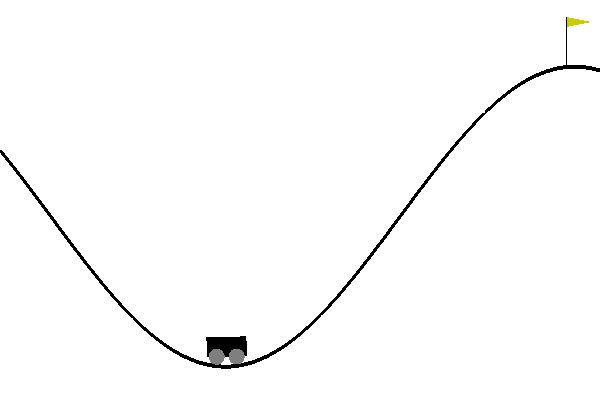
\includegraphics[width=0.9\linewidth]{img/MountainCar-0.png}
            \caption{}
            \label{MountainCar-0 states:a}
        \end{subfigure}%
        \begin{subfigure}{0.5\linewidth}
            \centering
            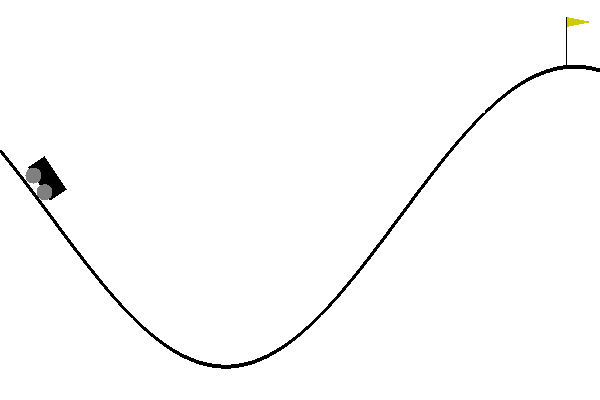
\includegraphics[width=0.9\linewidth]{img/MountainCar-1.png}
            \caption{}
            \label{MountainCar-0 states:b}
        \end{subfigure}
        \begin{subfigure}{0.5\linewidth}
            \centering
            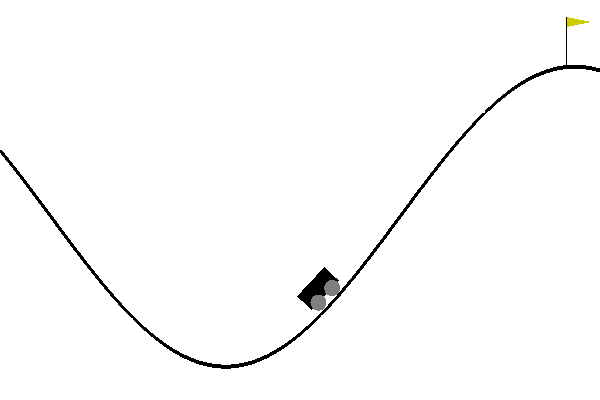
\includegraphics[width=0.9\linewidth]{img/MountainCar-2.png}
            \caption{}
            \label{MountainCar-0 states:c}
        \end{subfigure}%
        \begin{subfigure}{0.5\linewidth}
            \centering
            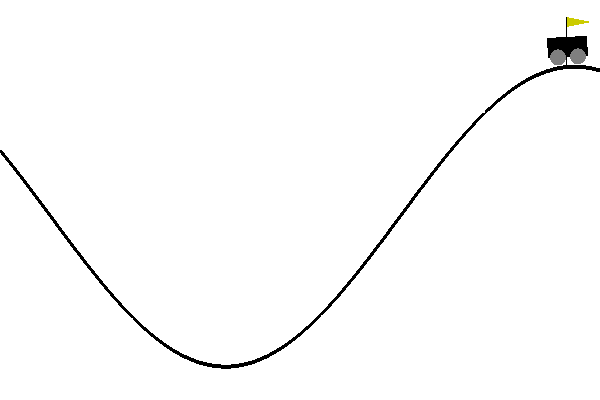
\includegraphics[width=0.9\linewidth]{img/MountainCar-3.png}
            \caption{}
            \label{MountainCar-0 states:d}
        \end{subfigure}
        \caption{Some of the possible states of the environments MountainCar-v0 and MountainCarContinuous-v0. The objective is to the car to reach the right end of the screen. If the agent move outside the left end of the screen, the simulation is terminated as failed. The starting pointing is in a random position near the state \figref{MountainCar-0 states:a}.}
        \label{MountainCar-0 states}
    \end{minipage}
\end{table*}

The results are shown as 3 curves by episodes: cumulative goals reached, rewards, and exploration rate; for each environment simulation.
The cumulative goals reached shows the total of how many times the goal of the environment was achieved by the agent within the limit steps preconfigured by the library.
Similarly, the reward shows the return of the environment, while the exploitation rate shows the evolution of that variable over episodes.

\figref{results_FrozenLakeNoSlip-v0} shows the results for FrozenLakeNoSlip-v0.
Since this is a discrete deterministic environment, the states are updates in a Markov chain.
The curves demonstrate constant cumulative goals reached slope and the fast saturation of the rewards.
This presents the {\Qlearning} algorithm was not only able to succeed in most of the episodes but also had fast training to the optimal solution.

\begin{figure*}[!t]
    \centering
    %% Creator: Matplotlib, PGF backend
%%
%% To include the figure in your LaTeX document, write
%%   \input{<filename>.pgf}
%%
%% Make sure the required packages are loaded in your preamble
%%   \usepackage{pgf}
%%
%% Figures using additional raster images can only be included by \input if
%% they are in the same directory as the main LaTeX file. For loading figures
%% from other directories you can use the `import` package
%%   \usepackage{import}
%% and then include the figures with
%%   \import{<path to file>}{<filename>.pgf}
%%
%% Matplotlib used the following preamble
%%
\begingroup%
\makeatletter%
\begin{pgfpicture}%
\pgfpathrectangle{\pgfpointorigin}{\pgfqpoint{7.000000in}{2.250000in}}%
\pgfusepath{use as bounding box, clip}%
\begin{pgfscope}%
\pgfsetbuttcap%
\pgfsetmiterjoin%
\definecolor{currentfill}{rgb}{1.000000,1.000000,1.000000}%
\pgfsetfillcolor{currentfill}%
\pgfsetlinewidth{0.000000pt}%
\definecolor{currentstroke}{rgb}{1.000000,1.000000,1.000000}%
\pgfsetstrokecolor{currentstroke}%
\pgfsetdash{}{0pt}%
\pgfpathmoveto{\pgfqpoint{0.000000in}{0.000000in}}%
\pgfpathlineto{\pgfqpoint{7.000000in}{0.000000in}}%
\pgfpathlineto{\pgfqpoint{7.000000in}{2.250000in}}%
\pgfpathlineto{\pgfqpoint{0.000000in}{2.250000in}}%
\pgfpathclose%
\pgfusepath{fill}%
\end{pgfscope}%
\begin{pgfscope}%
\pgfpathrectangle{\pgfqpoint{0.665215in}{0.469571in}}{\pgfqpoint{5.056081in}{1.621993in}}%
\pgfusepath{clip}%
\pgfsetbuttcap%
\pgfsetroundjoin%
\definecolor{currentfill}{rgb}{0.000000,0.627451,0.000000}%
\pgfsetfillcolor{currentfill}%
\pgfsetfillopacity{0.200000}%
\pgfsetlinewidth{0.000000pt}%
\definecolor{currentstroke}{rgb}{0.000000,0.627451,0.000000}%
\pgfsetstrokecolor{currentstroke}%
\pgfsetstrokeopacity{0.200000}%
\pgfsetdash{}{0pt}%
\pgfpathmoveto{\pgfqpoint{0.665215in}{2.075344in}}%
\pgfpathlineto{\pgfqpoint{0.665215in}{2.075344in}}%
\pgfpathlineto{\pgfqpoint{0.685520in}{1.057336in}}%
\pgfpathlineto{\pgfqpoint{0.705826in}{0.684712in}}%
\pgfpathlineto{\pgfqpoint{0.726131in}{0.548319in}}%
\pgfpathlineto{\pgfqpoint{0.746437in}{0.498395in}}%
\pgfpathlineto{\pgfqpoint{0.766742in}{0.480121in}}%
\pgfpathlineto{\pgfqpoint{0.787048in}{0.473433in}}%
\pgfpathlineto{\pgfqpoint{0.807354in}{0.470984in}}%
\pgfpathlineto{\pgfqpoint{0.827659in}{0.470088in}}%
\pgfpathlineto{\pgfqpoint{0.847965in}{0.469760in}}%
\pgfpathlineto{\pgfqpoint{0.868270in}{0.469640in}}%
\pgfpathlineto{\pgfqpoint{0.888576in}{0.469596in}}%
\pgfpathlineto{\pgfqpoint{0.908881in}{0.469580in}}%
\pgfpathlineto{\pgfqpoint{0.929187in}{0.469574in}}%
\pgfpathlineto{\pgfqpoint{0.949492in}{0.469572in}}%
\pgfpathlineto{\pgfqpoint{0.969798in}{0.469571in}}%
\pgfpathlineto{\pgfqpoint{0.990103in}{0.469571in}}%
\pgfpathlineto{\pgfqpoint{1.010409in}{0.469571in}}%
\pgfpathlineto{\pgfqpoint{1.030715in}{0.469571in}}%
\pgfpathlineto{\pgfqpoint{1.051020in}{0.469571in}}%
\pgfpathlineto{\pgfqpoint{1.071326in}{0.469571in}}%
\pgfpathlineto{\pgfqpoint{1.091631in}{0.469571in}}%
\pgfpathlineto{\pgfqpoint{1.111937in}{0.469571in}}%
\pgfpathlineto{\pgfqpoint{1.132242in}{0.469571in}}%
\pgfpathlineto{\pgfqpoint{1.152548in}{0.469571in}}%
\pgfpathlineto{\pgfqpoint{1.172853in}{0.469571in}}%
\pgfpathlineto{\pgfqpoint{1.193159in}{0.469571in}}%
\pgfpathlineto{\pgfqpoint{1.213464in}{0.469571in}}%
\pgfpathlineto{\pgfqpoint{1.233770in}{0.469571in}}%
\pgfpathlineto{\pgfqpoint{1.254076in}{0.469571in}}%
\pgfpathlineto{\pgfqpoint{1.274381in}{0.469571in}}%
\pgfpathlineto{\pgfqpoint{1.294687in}{0.469571in}}%
\pgfpathlineto{\pgfqpoint{1.314992in}{0.469571in}}%
\pgfpathlineto{\pgfqpoint{1.335298in}{0.469571in}}%
\pgfpathlineto{\pgfqpoint{1.355603in}{0.469571in}}%
\pgfpathlineto{\pgfqpoint{1.375909in}{0.469571in}}%
\pgfpathlineto{\pgfqpoint{1.396214in}{0.469571in}}%
\pgfpathlineto{\pgfqpoint{1.416520in}{0.469571in}}%
\pgfpathlineto{\pgfqpoint{1.436825in}{0.469571in}}%
\pgfpathlineto{\pgfqpoint{1.457131in}{0.469571in}}%
\pgfpathlineto{\pgfqpoint{1.477437in}{0.469571in}}%
\pgfpathlineto{\pgfqpoint{1.497742in}{0.469571in}}%
\pgfpathlineto{\pgfqpoint{1.518048in}{0.469571in}}%
\pgfpathlineto{\pgfqpoint{1.538353in}{0.469571in}}%
\pgfpathlineto{\pgfqpoint{1.558659in}{0.469571in}}%
\pgfpathlineto{\pgfqpoint{1.578964in}{0.469571in}}%
\pgfpathlineto{\pgfqpoint{1.599270in}{0.469571in}}%
\pgfpathlineto{\pgfqpoint{1.619575in}{0.469571in}}%
\pgfpathlineto{\pgfqpoint{1.639881in}{0.469571in}}%
\pgfpathlineto{\pgfqpoint{1.660186in}{0.469571in}}%
\pgfpathlineto{\pgfqpoint{1.680492in}{0.469571in}}%
\pgfpathlineto{\pgfqpoint{1.700798in}{0.469571in}}%
\pgfpathlineto{\pgfqpoint{1.721103in}{0.469571in}}%
\pgfpathlineto{\pgfqpoint{1.741409in}{0.469571in}}%
\pgfpathlineto{\pgfqpoint{1.761714in}{0.469571in}}%
\pgfpathlineto{\pgfqpoint{1.782020in}{0.469571in}}%
\pgfpathlineto{\pgfqpoint{1.802325in}{0.469571in}}%
\pgfpathlineto{\pgfqpoint{1.822631in}{0.469571in}}%
\pgfpathlineto{\pgfqpoint{1.842936in}{0.469571in}}%
\pgfpathlineto{\pgfqpoint{1.863242in}{0.469571in}}%
\pgfpathlineto{\pgfqpoint{1.883547in}{0.469571in}}%
\pgfpathlineto{\pgfqpoint{1.903853in}{0.469571in}}%
\pgfpathlineto{\pgfqpoint{1.924159in}{0.469571in}}%
\pgfpathlineto{\pgfqpoint{1.944464in}{0.469571in}}%
\pgfpathlineto{\pgfqpoint{1.964770in}{0.469571in}}%
\pgfpathlineto{\pgfqpoint{1.985075in}{0.469571in}}%
\pgfpathlineto{\pgfqpoint{2.005381in}{0.469571in}}%
\pgfpathlineto{\pgfqpoint{2.025686in}{0.469571in}}%
\pgfpathlineto{\pgfqpoint{2.045992in}{0.469571in}}%
\pgfpathlineto{\pgfqpoint{2.066297in}{0.469571in}}%
\pgfpathlineto{\pgfqpoint{2.086603in}{0.469571in}}%
\pgfpathlineto{\pgfqpoint{2.106909in}{0.469571in}}%
\pgfpathlineto{\pgfqpoint{2.127214in}{0.469571in}}%
\pgfpathlineto{\pgfqpoint{2.147520in}{0.469571in}}%
\pgfpathlineto{\pgfqpoint{2.167825in}{0.469571in}}%
\pgfpathlineto{\pgfqpoint{2.188131in}{0.469571in}}%
\pgfpathlineto{\pgfqpoint{2.208436in}{0.469571in}}%
\pgfpathlineto{\pgfqpoint{2.228742in}{0.469571in}}%
\pgfpathlineto{\pgfqpoint{2.249047in}{0.469571in}}%
\pgfpathlineto{\pgfqpoint{2.269353in}{0.469571in}}%
\pgfpathlineto{\pgfqpoint{2.289658in}{0.469571in}}%
\pgfpathlineto{\pgfqpoint{2.309964in}{0.469571in}}%
\pgfpathlineto{\pgfqpoint{2.330270in}{0.469571in}}%
\pgfpathlineto{\pgfqpoint{2.350575in}{0.469571in}}%
\pgfpathlineto{\pgfqpoint{2.370881in}{0.469571in}}%
\pgfpathlineto{\pgfqpoint{2.391186in}{0.469571in}}%
\pgfpathlineto{\pgfqpoint{2.411492in}{0.469571in}}%
\pgfpathlineto{\pgfqpoint{2.431797in}{0.469571in}}%
\pgfpathlineto{\pgfqpoint{2.452103in}{0.469571in}}%
\pgfpathlineto{\pgfqpoint{2.472408in}{0.469571in}}%
\pgfpathlineto{\pgfqpoint{2.492714in}{0.469571in}}%
\pgfpathlineto{\pgfqpoint{2.513019in}{0.469571in}}%
\pgfpathlineto{\pgfqpoint{2.533325in}{0.469571in}}%
\pgfpathlineto{\pgfqpoint{2.553631in}{0.469571in}}%
\pgfpathlineto{\pgfqpoint{2.573936in}{0.469571in}}%
\pgfpathlineto{\pgfqpoint{2.594242in}{0.469571in}}%
\pgfpathlineto{\pgfqpoint{2.614547in}{0.469571in}}%
\pgfpathlineto{\pgfqpoint{2.634853in}{0.469571in}}%
\pgfpathlineto{\pgfqpoint{2.655158in}{0.469571in}}%
\pgfpathlineto{\pgfqpoint{2.675464in}{0.469571in}}%
\pgfpathlineto{\pgfqpoint{2.695769in}{0.469571in}}%
\pgfpathlineto{\pgfqpoint{2.716075in}{0.469571in}}%
\pgfpathlineto{\pgfqpoint{2.736380in}{0.469571in}}%
\pgfpathlineto{\pgfqpoint{2.756686in}{0.469571in}}%
\pgfpathlineto{\pgfqpoint{2.776992in}{0.469571in}}%
\pgfpathlineto{\pgfqpoint{2.797297in}{0.469571in}}%
\pgfpathlineto{\pgfqpoint{2.817603in}{0.469571in}}%
\pgfpathlineto{\pgfqpoint{2.837908in}{0.469571in}}%
\pgfpathlineto{\pgfqpoint{2.858214in}{0.469571in}}%
\pgfpathlineto{\pgfqpoint{2.878519in}{0.469571in}}%
\pgfpathlineto{\pgfqpoint{2.898825in}{0.469571in}}%
\pgfpathlineto{\pgfqpoint{2.919130in}{0.469571in}}%
\pgfpathlineto{\pgfqpoint{2.939436in}{0.469571in}}%
\pgfpathlineto{\pgfqpoint{2.959741in}{0.469571in}}%
\pgfpathlineto{\pgfqpoint{2.980047in}{0.469571in}}%
\pgfpathlineto{\pgfqpoint{3.000353in}{0.469571in}}%
\pgfpathlineto{\pgfqpoint{3.020658in}{0.469571in}}%
\pgfpathlineto{\pgfqpoint{3.040964in}{0.469571in}}%
\pgfpathlineto{\pgfqpoint{3.061269in}{0.469571in}}%
\pgfpathlineto{\pgfqpoint{3.081575in}{0.469571in}}%
\pgfpathlineto{\pgfqpoint{3.101880in}{0.469571in}}%
\pgfpathlineto{\pgfqpoint{3.122186in}{0.469571in}}%
\pgfpathlineto{\pgfqpoint{3.142491in}{0.469571in}}%
\pgfpathlineto{\pgfqpoint{3.162797in}{0.469571in}}%
\pgfpathlineto{\pgfqpoint{3.183102in}{0.469571in}}%
\pgfpathlineto{\pgfqpoint{3.203408in}{0.469571in}}%
\pgfpathlineto{\pgfqpoint{3.223714in}{0.469571in}}%
\pgfpathlineto{\pgfqpoint{3.244019in}{0.469571in}}%
\pgfpathlineto{\pgfqpoint{3.264325in}{0.469571in}}%
\pgfpathlineto{\pgfqpoint{3.284630in}{0.469571in}}%
\pgfpathlineto{\pgfqpoint{3.304936in}{0.469571in}}%
\pgfpathlineto{\pgfqpoint{3.325241in}{0.469571in}}%
\pgfpathlineto{\pgfqpoint{3.345547in}{0.469571in}}%
\pgfpathlineto{\pgfqpoint{3.365852in}{0.469571in}}%
\pgfpathlineto{\pgfqpoint{3.386158in}{0.469571in}}%
\pgfpathlineto{\pgfqpoint{3.406463in}{0.469571in}}%
\pgfpathlineto{\pgfqpoint{3.426769in}{0.469571in}}%
\pgfpathlineto{\pgfqpoint{3.447075in}{0.469571in}}%
\pgfpathlineto{\pgfqpoint{3.467380in}{0.469571in}}%
\pgfpathlineto{\pgfqpoint{3.487686in}{0.469571in}}%
\pgfpathlineto{\pgfqpoint{3.507991in}{0.469571in}}%
\pgfpathlineto{\pgfqpoint{3.528297in}{0.469571in}}%
\pgfpathlineto{\pgfqpoint{3.548602in}{0.469571in}}%
\pgfpathlineto{\pgfqpoint{3.568908in}{0.469571in}}%
\pgfpathlineto{\pgfqpoint{3.589213in}{0.469571in}}%
\pgfpathlineto{\pgfqpoint{3.609519in}{0.469571in}}%
\pgfpathlineto{\pgfqpoint{3.629824in}{0.469571in}}%
\pgfpathlineto{\pgfqpoint{3.650130in}{0.469571in}}%
\pgfpathlineto{\pgfqpoint{3.670436in}{0.469571in}}%
\pgfpathlineto{\pgfqpoint{3.690741in}{0.469571in}}%
\pgfpathlineto{\pgfqpoint{3.711047in}{0.469571in}}%
\pgfpathlineto{\pgfqpoint{3.731352in}{0.469571in}}%
\pgfpathlineto{\pgfqpoint{3.751658in}{0.469571in}}%
\pgfpathlineto{\pgfqpoint{3.771963in}{0.469571in}}%
\pgfpathlineto{\pgfqpoint{3.792269in}{0.469571in}}%
\pgfpathlineto{\pgfqpoint{3.812574in}{0.469571in}}%
\pgfpathlineto{\pgfqpoint{3.832880in}{0.469571in}}%
\pgfpathlineto{\pgfqpoint{3.853185in}{0.469571in}}%
\pgfpathlineto{\pgfqpoint{3.873491in}{0.469571in}}%
\pgfpathlineto{\pgfqpoint{3.893797in}{0.469571in}}%
\pgfpathlineto{\pgfqpoint{3.914102in}{0.469571in}}%
\pgfpathlineto{\pgfqpoint{3.934408in}{0.469571in}}%
\pgfpathlineto{\pgfqpoint{3.954713in}{0.469571in}}%
\pgfpathlineto{\pgfqpoint{3.975019in}{0.469571in}}%
\pgfpathlineto{\pgfqpoint{3.995324in}{0.469571in}}%
\pgfpathlineto{\pgfqpoint{4.015630in}{0.469571in}}%
\pgfpathlineto{\pgfqpoint{4.035935in}{0.469571in}}%
\pgfpathlineto{\pgfqpoint{4.056241in}{0.469571in}}%
\pgfpathlineto{\pgfqpoint{4.076546in}{0.469571in}}%
\pgfpathlineto{\pgfqpoint{4.096852in}{0.469571in}}%
\pgfpathlineto{\pgfqpoint{4.117158in}{0.469571in}}%
\pgfpathlineto{\pgfqpoint{4.137463in}{0.469571in}}%
\pgfpathlineto{\pgfqpoint{4.157769in}{0.469571in}}%
\pgfpathlineto{\pgfqpoint{4.178074in}{0.469571in}}%
\pgfpathlineto{\pgfqpoint{4.198380in}{0.469571in}}%
\pgfpathlineto{\pgfqpoint{4.218685in}{0.469571in}}%
\pgfpathlineto{\pgfqpoint{4.238991in}{0.469571in}}%
\pgfpathlineto{\pgfqpoint{4.259296in}{0.469571in}}%
\pgfpathlineto{\pgfqpoint{4.279602in}{0.469571in}}%
\pgfpathlineto{\pgfqpoint{4.299907in}{0.469571in}}%
\pgfpathlineto{\pgfqpoint{4.320213in}{0.469571in}}%
\pgfpathlineto{\pgfqpoint{4.340519in}{0.469571in}}%
\pgfpathlineto{\pgfqpoint{4.360824in}{0.469571in}}%
\pgfpathlineto{\pgfqpoint{4.381130in}{0.469571in}}%
\pgfpathlineto{\pgfqpoint{4.401435in}{0.469571in}}%
\pgfpathlineto{\pgfqpoint{4.421741in}{0.469571in}}%
\pgfpathlineto{\pgfqpoint{4.442046in}{0.469571in}}%
\pgfpathlineto{\pgfqpoint{4.462352in}{0.469571in}}%
\pgfpathlineto{\pgfqpoint{4.482657in}{0.469571in}}%
\pgfpathlineto{\pgfqpoint{4.502963in}{0.469571in}}%
\pgfpathlineto{\pgfqpoint{4.523268in}{0.469571in}}%
\pgfpathlineto{\pgfqpoint{4.543574in}{0.469571in}}%
\pgfpathlineto{\pgfqpoint{4.563880in}{0.469571in}}%
\pgfpathlineto{\pgfqpoint{4.584185in}{0.469571in}}%
\pgfpathlineto{\pgfqpoint{4.604491in}{0.469571in}}%
\pgfpathlineto{\pgfqpoint{4.624796in}{0.469571in}}%
\pgfpathlineto{\pgfqpoint{4.645102in}{0.469571in}}%
\pgfpathlineto{\pgfqpoint{4.665407in}{0.469571in}}%
\pgfpathlineto{\pgfqpoint{4.685713in}{0.469571in}}%
\pgfpathlineto{\pgfqpoint{4.706018in}{0.469571in}}%
\pgfpathlineto{\pgfqpoint{4.726324in}{0.469571in}}%
\pgfpathlineto{\pgfqpoint{4.746629in}{0.469571in}}%
\pgfpathlineto{\pgfqpoint{4.766935in}{0.469571in}}%
\pgfpathlineto{\pgfqpoint{4.787241in}{0.469571in}}%
\pgfpathlineto{\pgfqpoint{4.807546in}{0.469571in}}%
\pgfpathlineto{\pgfqpoint{4.827852in}{0.469571in}}%
\pgfpathlineto{\pgfqpoint{4.848157in}{0.469571in}}%
\pgfpathlineto{\pgfqpoint{4.868463in}{0.469571in}}%
\pgfpathlineto{\pgfqpoint{4.888768in}{0.469571in}}%
\pgfpathlineto{\pgfqpoint{4.909074in}{0.469571in}}%
\pgfpathlineto{\pgfqpoint{4.929379in}{0.469571in}}%
\pgfpathlineto{\pgfqpoint{4.949685in}{0.469571in}}%
\pgfpathlineto{\pgfqpoint{4.969990in}{0.469571in}}%
\pgfpathlineto{\pgfqpoint{4.990296in}{0.469571in}}%
\pgfpathlineto{\pgfqpoint{5.010602in}{0.469571in}}%
\pgfpathlineto{\pgfqpoint{5.030907in}{0.469571in}}%
\pgfpathlineto{\pgfqpoint{5.051213in}{0.469571in}}%
\pgfpathlineto{\pgfqpoint{5.071518in}{0.469571in}}%
\pgfpathlineto{\pgfqpoint{5.091824in}{0.469571in}}%
\pgfpathlineto{\pgfqpoint{5.112129in}{0.469571in}}%
\pgfpathlineto{\pgfqpoint{5.132435in}{0.469571in}}%
\pgfpathlineto{\pgfqpoint{5.152740in}{0.469571in}}%
\pgfpathlineto{\pgfqpoint{5.173046in}{0.469571in}}%
\pgfpathlineto{\pgfqpoint{5.193351in}{0.469571in}}%
\pgfpathlineto{\pgfqpoint{5.213657in}{0.469571in}}%
\pgfpathlineto{\pgfqpoint{5.233963in}{0.469571in}}%
\pgfpathlineto{\pgfqpoint{5.254268in}{0.469571in}}%
\pgfpathlineto{\pgfqpoint{5.274574in}{0.469571in}}%
\pgfpathlineto{\pgfqpoint{5.294879in}{0.469571in}}%
\pgfpathlineto{\pgfqpoint{5.315185in}{0.469571in}}%
\pgfpathlineto{\pgfqpoint{5.335490in}{0.469571in}}%
\pgfpathlineto{\pgfqpoint{5.355796in}{0.469571in}}%
\pgfpathlineto{\pgfqpoint{5.376101in}{0.469571in}}%
\pgfpathlineto{\pgfqpoint{5.396407in}{0.469571in}}%
\pgfpathlineto{\pgfqpoint{5.416712in}{0.469571in}}%
\pgfpathlineto{\pgfqpoint{5.437018in}{0.469571in}}%
\pgfpathlineto{\pgfqpoint{5.457324in}{0.469571in}}%
\pgfpathlineto{\pgfqpoint{5.477629in}{0.469571in}}%
\pgfpathlineto{\pgfqpoint{5.497935in}{0.469571in}}%
\pgfpathlineto{\pgfqpoint{5.518240in}{0.469571in}}%
\pgfpathlineto{\pgfqpoint{5.538546in}{0.469571in}}%
\pgfpathlineto{\pgfqpoint{5.558851in}{0.469571in}}%
\pgfpathlineto{\pgfqpoint{5.579157in}{0.469571in}}%
\pgfpathlineto{\pgfqpoint{5.599462in}{0.469571in}}%
\pgfpathlineto{\pgfqpoint{5.619768in}{0.469571in}}%
\pgfpathlineto{\pgfqpoint{5.640073in}{0.469571in}}%
\pgfpathlineto{\pgfqpoint{5.660379in}{0.469571in}}%
\pgfpathlineto{\pgfqpoint{5.680685in}{0.469571in}}%
\pgfpathlineto{\pgfqpoint{5.700990in}{0.469571in}}%
\pgfpathlineto{\pgfqpoint{5.721296in}{0.469571in}}%
\pgfpathlineto{\pgfqpoint{5.721296in}{0.469571in}}%
\pgfpathlineto{\pgfqpoint{5.721296in}{0.469571in}}%
\pgfpathlineto{\pgfqpoint{5.700990in}{0.469571in}}%
\pgfpathlineto{\pgfqpoint{5.680685in}{0.469571in}}%
\pgfpathlineto{\pgfqpoint{5.660379in}{0.469571in}}%
\pgfpathlineto{\pgfqpoint{5.640073in}{0.469571in}}%
\pgfpathlineto{\pgfqpoint{5.619768in}{0.469571in}}%
\pgfpathlineto{\pgfqpoint{5.599462in}{0.469571in}}%
\pgfpathlineto{\pgfqpoint{5.579157in}{0.469571in}}%
\pgfpathlineto{\pgfqpoint{5.558851in}{0.469571in}}%
\pgfpathlineto{\pgfqpoint{5.538546in}{0.469571in}}%
\pgfpathlineto{\pgfqpoint{5.518240in}{0.469571in}}%
\pgfpathlineto{\pgfqpoint{5.497935in}{0.469571in}}%
\pgfpathlineto{\pgfqpoint{5.477629in}{0.469571in}}%
\pgfpathlineto{\pgfqpoint{5.457324in}{0.469571in}}%
\pgfpathlineto{\pgfqpoint{5.437018in}{0.469571in}}%
\pgfpathlineto{\pgfqpoint{5.416712in}{0.469571in}}%
\pgfpathlineto{\pgfqpoint{5.396407in}{0.469571in}}%
\pgfpathlineto{\pgfqpoint{5.376101in}{0.469571in}}%
\pgfpathlineto{\pgfqpoint{5.355796in}{0.469571in}}%
\pgfpathlineto{\pgfqpoint{5.335490in}{0.469571in}}%
\pgfpathlineto{\pgfqpoint{5.315185in}{0.469571in}}%
\pgfpathlineto{\pgfqpoint{5.294879in}{0.469571in}}%
\pgfpathlineto{\pgfqpoint{5.274574in}{0.469571in}}%
\pgfpathlineto{\pgfqpoint{5.254268in}{0.469571in}}%
\pgfpathlineto{\pgfqpoint{5.233963in}{0.469571in}}%
\pgfpathlineto{\pgfqpoint{5.213657in}{0.469571in}}%
\pgfpathlineto{\pgfqpoint{5.193351in}{0.469571in}}%
\pgfpathlineto{\pgfqpoint{5.173046in}{0.469571in}}%
\pgfpathlineto{\pgfqpoint{5.152740in}{0.469571in}}%
\pgfpathlineto{\pgfqpoint{5.132435in}{0.469571in}}%
\pgfpathlineto{\pgfqpoint{5.112129in}{0.469571in}}%
\pgfpathlineto{\pgfqpoint{5.091824in}{0.469571in}}%
\pgfpathlineto{\pgfqpoint{5.071518in}{0.469571in}}%
\pgfpathlineto{\pgfqpoint{5.051213in}{0.469571in}}%
\pgfpathlineto{\pgfqpoint{5.030907in}{0.469571in}}%
\pgfpathlineto{\pgfqpoint{5.010602in}{0.469571in}}%
\pgfpathlineto{\pgfqpoint{4.990296in}{0.469571in}}%
\pgfpathlineto{\pgfqpoint{4.969990in}{0.469571in}}%
\pgfpathlineto{\pgfqpoint{4.949685in}{0.469571in}}%
\pgfpathlineto{\pgfqpoint{4.929379in}{0.469571in}}%
\pgfpathlineto{\pgfqpoint{4.909074in}{0.469571in}}%
\pgfpathlineto{\pgfqpoint{4.888768in}{0.469571in}}%
\pgfpathlineto{\pgfqpoint{4.868463in}{0.469571in}}%
\pgfpathlineto{\pgfqpoint{4.848157in}{0.469571in}}%
\pgfpathlineto{\pgfqpoint{4.827852in}{0.469571in}}%
\pgfpathlineto{\pgfqpoint{4.807546in}{0.469571in}}%
\pgfpathlineto{\pgfqpoint{4.787241in}{0.469571in}}%
\pgfpathlineto{\pgfqpoint{4.766935in}{0.469571in}}%
\pgfpathlineto{\pgfqpoint{4.746629in}{0.469571in}}%
\pgfpathlineto{\pgfqpoint{4.726324in}{0.469571in}}%
\pgfpathlineto{\pgfqpoint{4.706018in}{0.469571in}}%
\pgfpathlineto{\pgfqpoint{4.685713in}{0.469571in}}%
\pgfpathlineto{\pgfqpoint{4.665407in}{0.469571in}}%
\pgfpathlineto{\pgfqpoint{4.645102in}{0.469571in}}%
\pgfpathlineto{\pgfqpoint{4.624796in}{0.469571in}}%
\pgfpathlineto{\pgfqpoint{4.604491in}{0.469571in}}%
\pgfpathlineto{\pgfqpoint{4.584185in}{0.469571in}}%
\pgfpathlineto{\pgfqpoint{4.563880in}{0.469571in}}%
\pgfpathlineto{\pgfqpoint{4.543574in}{0.469571in}}%
\pgfpathlineto{\pgfqpoint{4.523268in}{0.469571in}}%
\pgfpathlineto{\pgfqpoint{4.502963in}{0.469571in}}%
\pgfpathlineto{\pgfqpoint{4.482657in}{0.469571in}}%
\pgfpathlineto{\pgfqpoint{4.462352in}{0.469571in}}%
\pgfpathlineto{\pgfqpoint{4.442046in}{0.469571in}}%
\pgfpathlineto{\pgfqpoint{4.421741in}{0.469571in}}%
\pgfpathlineto{\pgfqpoint{4.401435in}{0.469571in}}%
\pgfpathlineto{\pgfqpoint{4.381130in}{0.469571in}}%
\pgfpathlineto{\pgfqpoint{4.360824in}{0.469571in}}%
\pgfpathlineto{\pgfqpoint{4.340519in}{0.469571in}}%
\pgfpathlineto{\pgfqpoint{4.320213in}{0.469571in}}%
\pgfpathlineto{\pgfqpoint{4.299907in}{0.469571in}}%
\pgfpathlineto{\pgfqpoint{4.279602in}{0.469571in}}%
\pgfpathlineto{\pgfqpoint{4.259296in}{0.469571in}}%
\pgfpathlineto{\pgfqpoint{4.238991in}{0.469571in}}%
\pgfpathlineto{\pgfqpoint{4.218685in}{0.469571in}}%
\pgfpathlineto{\pgfqpoint{4.198380in}{0.469571in}}%
\pgfpathlineto{\pgfqpoint{4.178074in}{0.469571in}}%
\pgfpathlineto{\pgfqpoint{4.157769in}{0.469571in}}%
\pgfpathlineto{\pgfqpoint{4.137463in}{0.469571in}}%
\pgfpathlineto{\pgfqpoint{4.117158in}{0.469571in}}%
\pgfpathlineto{\pgfqpoint{4.096852in}{0.469571in}}%
\pgfpathlineto{\pgfqpoint{4.076546in}{0.469571in}}%
\pgfpathlineto{\pgfqpoint{4.056241in}{0.469571in}}%
\pgfpathlineto{\pgfqpoint{4.035935in}{0.469571in}}%
\pgfpathlineto{\pgfqpoint{4.015630in}{0.469571in}}%
\pgfpathlineto{\pgfqpoint{3.995324in}{0.469571in}}%
\pgfpathlineto{\pgfqpoint{3.975019in}{0.469571in}}%
\pgfpathlineto{\pgfqpoint{3.954713in}{0.469571in}}%
\pgfpathlineto{\pgfqpoint{3.934408in}{0.469571in}}%
\pgfpathlineto{\pgfqpoint{3.914102in}{0.469571in}}%
\pgfpathlineto{\pgfqpoint{3.893797in}{0.469571in}}%
\pgfpathlineto{\pgfqpoint{3.873491in}{0.469571in}}%
\pgfpathlineto{\pgfqpoint{3.853185in}{0.469571in}}%
\pgfpathlineto{\pgfqpoint{3.832880in}{0.469571in}}%
\pgfpathlineto{\pgfqpoint{3.812574in}{0.469571in}}%
\pgfpathlineto{\pgfqpoint{3.792269in}{0.469571in}}%
\pgfpathlineto{\pgfqpoint{3.771963in}{0.469571in}}%
\pgfpathlineto{\pgfqpoint{3.751658in}{0.469571in}}%
\pgfpathlineto{\pgfqpoint{3.731352in}{0.469571in}}%
\pgfpathlineto{\pgfqpoint{3.711047in}{0.469571in}}%
\pgfpathlineto{\pgfqpoint{3.690741in}{0.469571in}}%
\pgfpathlineto{\pgfqpoint{3.670436in}{0.469571in}}%
\pgfpathlineto{\pgfqpoint{3.650130in}{0.469571in}}%
\pgfpathlineto{\pgfqpoint{3.629824in}{0.469571in}}%
\pgfpathlineto{\pgfqpoint{3.609519in}{0.469571in}}%
\pgfpathlineto{\pgfqpoint{3.589213in}{0.469571in}}%
\pgfpathlineto{\pgfqpoint{3.568908in}{0.469571in}}%
\pgfpathlineto{\pgfqpoint{3.548602in}{0.469571in}}%
\pgfpathlineto{\pgfqpoint{3.528297in}{0.469571in}}%
\pgfpathlineto{\pgfqpoint{3.507991in}{0.469571in}}%
\pgfpathlineto{\pgfqpoint{3.487686in}{0.469571in}}%
\pgfpathlineto{\pgfqpoint{3.467380in}{0.469571in}}%
\pgfpathlineto{\pgfqpoint{3.447075in}{0.469571in}}%
\pgfpathlineto{\pgfqpoint{3.426769in}{0.469571in}}%
\pgfpathlineto{\pgfqpoint{3.406463in}{0.469571in}}%
\pgfpathlineto{\pgfqpoint{3.386158in}{0.469571in}}%
\pgfpathlineto{\pgfqpoint{3.365852in}{0.469571in}}%
\pgfpathlineto{\pgfqpoint{3.345547in}{0.469571in}}%
\pgfpathlineto{\pgfqpoint{3.325241in}{0.469571in}}%
\pgfpathlineto{\pgfqpoint{3.304936in}{0.469571in}}%
\pgfpathlineto{\pgfqpoint{3.284630in}{0.469571in}}%
\pgfpathlineto{\pgfqpoint{3.264325in}{0.469571in}}%
\pgfpathlineto{\pgfqpoint{3.244019in}{0.469571in}}%
\pgfpathlineto{\pgfqpoint{3.223714in}{0.469571in}}%
\pgfpathlineto{\pgfqpoint{3.203408in}{0.469571in}}%
\pgfpathlineto{\pgfqpoint{3.183102in}{0.469571in}}%
\pgfpathlineto{\pgfqpoint{3.162797in}{0.469571in}}%
\pgfpathlineto{\pgfqpoint{3.142491in}{0.469571in}}%
\pgfpathlineto{\pgfqpoint{3.122186in}{0.469571in}}%
\pgfpathlineto{\pgfqpoint{3.101880in}{0.469571in}}%
\pgfpathlineto{\pgfqpoint{3.081575in}{0.469571in}}%
\pgfpathlineto{\pgfqpoint{3.061269in}{0.469571in}}%
\pgfpathlineto{\pgfqpoint{3.040964in}{0.469571in}}%
\pgfpathlineto{\pgfqpoint{3.020658in}{0.469571in}}%
\pgfpathlineto{\pgfqpoint{3.000353in}{0.469571in}}%
\pgfpathlineto{\pgfqpoint{2.980047in}{0.469571in}}%
\pgfpathlineto{\pgfqpoint{2.959741in}{0.469571in}}%
\pgfpathlineto{\pgfqpoint{2.939436in}{0.469571in}}%
\pgfpathlineto{\pgfqpoint{2.919130in}{0.469571in}}%
\pgfpathlineto{\pgfqpoint{2.898825in}{0.469571in}}%
\pgfpathlineto{\pgfqpoint{2.878519in}{0.469571in}}%
\pgfpathlineto{\pgfqpoint{2.858214in}{0.469571in}}%
\pgfpathlineto{\pgfqpoint{2.837908in}{0.469571in}}%
\pgfpathlineto{\pgfqpoint{2.817603in}{0.469571in}}%
\pgfpathlineto{\pgfqpoint{2.797297in}{0.469571in}}%
\pgfpathlineto{\pgfqpoint{2.776992in}{0.469571in}}%
\pgfpathlineto{\pgfqpoint{2.756686in}{0.469571in}}%
\pgfpathlineto{\pgfqpoint{2.736380in}{0.469571in}}%
\pgfpathlineto{\pgfqpoint{2.716075in}{0.469571in}}%
\pgfpathlineto{\pgfqpoint{2.695769in}{0.469571in}}%
\pgfpathlineto{\pgfqpoint{2.675464in}{0.469571in}}%
\pgfpathlineto{\pgfqpoint{2.655158in}{0.469571in}}%
\pgfpathlineto{\pgfqpoint{2.634853in}{0.469571in}}%
\pgfpathlineto{\pgfqpoint{2.614547in}{0.469571in}}%
\pgfpathlineto{\pgfqpoint{2.594242in}{0.469571in}}%
\pgfpathlineto{\pgfqpoint{2.573936in}{0.469571in}}%
\pgfpathlineto{\pgfqpoint{2.553631in}{0.469571in}}%
\pgfpathlineto{\pgfqpoint{2.533325in}{0.469571in}}%
\pgfpathlineto{\pgfqpoint{2.513019in}{0.469571in}}%
\pgfpathlineto{\pgfqpoint{2.492714in}{0.469571in}}%
\pgfpathlineto{\pgfqpoint{2.472408in}{0.469571in}}%
\pgfpathlineto{\pgfqpoint{2.452103in}{0.469571in}}%
\pgfpathlineto{\pgfqpoint{2.431797in}{0.469571in}}%
\pgfpathlineto{\pgfqpoint{2.411492in}{0.469571in}}%
\pgfpathlineto{\pgfqpoint{2.391186in}{0.469571in}}%
\pgfpathlineto{\pgfqpoint{2.370881in}{0.469571in}}%
\pgfpathlineto{\pgfqpoint{2.350575in}{0.469571in}}%
\pgfpathlineto{\pgfqpoint{2.330270in}{0.469571in}}%
\pgfpathlineto{\pgfqpoint{2.309964in}{0.469571in}}%
\pgfpathlineto{\pgfqpoint{2.289658in}{0.469571in}}%
\pgfpathlineto{\pgfqpoint{2.269353in}{0.469571in}}%
\pgfpathlineto{\pgfqpoint{2.249047in}{0.469571in}}%
\pgfpathlineto{\pgfqpoint{2.228742in}{0.469571in}}%
\pgfpathlineto{\pgfqpoint{2.208436in}{0.469571in}}%
\pgfpathlineto{\pgfqpoint{2.188131in}{0.469571in}}%
\pgfpathlineto{\pgfqpoint{2.167825in}{0.469571in}}%
\pgfpathlineto{\pgfqpoint{2.147520in}{0.469571in}}%
\pgfpathlineto{\pgfqpoint{2.127214in}{0.469571in}}%
\pgfpathlineto{\pgfqpoint{2.106909in}{0.469571in}}%
\pgfpathlineto{\pgfqpoint{2.086603in}{0.469571in}}%
\pgfpathlineto{\pgfqpoint{2.066297in}{0.469571in}}%
\pgfpathlineto{\pgfqpoint{2.045992in}{0.469571in}}%
\pgfpathlineto{\pgfqpoint{2.025686in}{0.469571in}}%
\pgfpathlineto{\pgfqpoint{2.005381in}{0.469571in}}%
\pgfpathlineto{\pgfqpoint{1.985075in}{0.469571in}}%
\pgfpathlineto{\pgfqpoint{1.964770in}{0.469571in}}%
\pgfpathlineto{\pgfqpoint{1.944464in}{0.469571in}}%
\pgfpathlineto{\pgfqpoint{1.924159in}{0.469571in}}%
\pgfpathlineto{\pgfqpoint{1.903853in}{0.469571in}}%
\pgfpathlineto{\pgfqpoint{1.883547in}{0.469571in}}%
\pgfpathlineto{\pgfqpoint{1.863242in}{0.469571in}}%
\pgfpathlineto{\pgfqpoint{1.842936in}{0.469571in}}%
\pgfpathlineto{\pgfqpoint{1.822631in}{0.469571in}}%
\pgfpathlineto{\pgfqpoint{1.802325in}{0.469571in}}%
\pgfpathlineto{\pgfqpoint{1.782020in}{0.469571in}}%
\pgfpathlineto{\pgfqpoint{1.761714in}{0.469571in}}%
\pgfpathlineto{\pgfqpoint{1.741409in}{0.469571in}}%
\pgfpathlineto{\pgfqpoint{1.721103in}{0.469571in}}%
\pgfpathlineto{\pgfqpoint{1.700798in}{0.469571in}}%
\pgfpathlineto{\pgfqpoint{1.680492in}{0.469571in}}%
\pgfpathlineto{\pgfqpoint{1.660186in}{0.469571in}}%
\pgfpathlineto{\pgfqpoint{1.639881in}{0.469571in}}%
\pgfpathlineto{\pgfqpoint{1.619575in}{0.469571in}}%
\pgfpathlineto{\pgfqpoint{1.599270in}{0.469571in}}%
\pgfpathlineto{\pgfqpoint{1.578964in}{0.469571in}}%
\pgfpathlineto{\pgfqpoint{1.558659in}{0.469571in}}%
\pgfpathlineto{\pgfqpoint{1.538353in}{0.469571in}}%
\pgfpathlineto{\pgfqpoint{1.518048in}{0.469571in}}%
\pgfpathlineto{\pgfqpoint{1.497742in}{0.469571in}}%
\pgfpathlineto{\pgfqpoint{1.477437in}{0.469571in}}%
\pgfpathlineto{\pgfqpoint{1.457131in}{0.469571in}}%
\pgfpathlineto{\pgfqpoint{1.436825in}{0.469571in}}%
\pgfpathlineto{\pgfqpoint{1.416520in}{0.469571in}}%
\pgfpathlineto{\pgfqpoint{1.396214in}{0.469571in}}%
\pgfpathlineto{\pgfqpoint{1.375909in}{0.469571in}}%
\pgfpathlineto{\pgfqpoint{1.355603in}{0.469571in}}%
\pgfpathlineto{\pgfqpoint{1.335298in}{0.469571in}}%
\pgfpathlineto{\pgfqpoint{1.314992in}{0.469571in}}%
\pgfpathlineto{\pgfqpoint{1.294687in}{0.469571in}}%
\pgfpathlineto{\pgfqpoint{1.274381in}{0.469571in}}%
\pgfpathlineto{\pgfqpoint{1.254076in}{0.469571in}}%
\pgfpathlineto{\pgfqpoint{1.233770in}{0.469571in}}%
\pgfpathlineto{\pgfqpoint{1.213464in}{0.469571in}}%
\pgfpathlineto{\pgfqpoint{1.193159in}{0.469571in}}%
\pgfpathlineto{\pgfqpoint{1.172853in}{0.469571in}}%
\pgfpathlineto{\pgfqpoint{1.152548in}{0.469571in}}%
\pgfpathlineto{\pgfqpoint{1.132242in}{0.469571in}}%
\pgfpathlineto{\pgfqpoint{1.111937in}{0.469571in}}%
\pgfpathlineto{\pgfqpoint{1.091631in}{0.469571in}}%
\pgfpathlineto{\pgfqpoint{1.071326in}{0.469571in}}%
\pgfpathlineto{\pgfqpoint{1.051020in}{0.469571in}}%
\pgfpathlineto{\pgfqpoint{1.030715in}{0.469571in}}%
\pgfpathlineto{\pgfqpoint{1.010409in}{0.469571in}}%
\pgfpathlineto{\pgfqpoint{0.990103in}{0.469571in}}%
\pgfpathlineto{\pgfqpoint{0.969798in}{0.469572in}}%
\pgfpathlineto{\pgfqpoint{0.949492in}{0.469574in}}%
\pgfpathlineto{\pgfqpoint{0.929187in}{0.469580in}}%
\pgfpathlineto{\pgfqpoint{0.908881in}{0.469596in}}%
\pgfpathlineto{\pgfqpoint{0.888576in}{0.469639in}}%
\pgfpathlineto{\pgfqpoint{0.868270in}{0.469758in}}%
\pgfpathlineto{\pgfqpoint{0.847965in}{0.470083in}}%
\pgfpathlineto{\pgfqpoint{0.827659in}{0.470970in}}%
\pgfpathlineto{\pgfqpoint{0.807354in}{0.473394in}}%
\pgfpathlineto{\pgfqpoint{0.787048in}{0.480016in}}%
\pgfpathlineto{\pgfqpoint{0.766742in}{0.498107in}}%
\pgfpathlineto{\pgfqpoint{0.746437in}{0.547532in}}%
\pgfpathlineto{\pgfqpoint{0.726131in}{0.682560in}}%
\pgfpathlineto{\pgfqpoint{0.705826in}{1.051458in}}%
\pgfpathlineto{\pgfqpoint{0.685520in}{2.059286in}}%
\pgfpathlineto{\pgfqpoint{0.665215in}{2.075344in}}%
\pgfpathclose%
\pgfusepath{fill}%
\end{pgfscope}%
\begin{pgfscope}%
\pgfpathrectangle{\pgfqpoint{0.665215in}{0.469571in}}{\pgfqpoint{5.056081in}{1.621993in}}%
\pgfusepath{clip}%
\pgfsetrectcap%
\pgfsetroundjoin%
\pgfsetlinewidth{1.505625pt}%
\definecolor{currentstroke}{rgb}{0.000000,0.627451,0.000000}%
\pgfsetstrokecolor{currentstroke}%
\pgfsetdash{}{0pt}%
\pgfpathmoveto{\pgfqpoint{0.665215in}{2.075344in}}%
\pgfpathlineto{\pgfqpoint{0.685520in}{1.477399in}}%
\pgfpathlineto{\pgfqpoint{0.705826in}{0.838468in}}%
\pgfpathlineto{\pgfqpoint{0.726131in}{0.604599in}}%
\pgfpathlineto{\pgfqpoint{0.746437in}{0.518996in}}%
\pgfpathlineto{\pgfqpoint{0.766742in}{0.487662in}}%
\pgfpathlineto{\pgfqpoint{0.787048in}{0.476193in}}%
\pgfpathlineto{\pgfqpoint{0.807354in}{0.471995in}}%
\pgfpathlineto{\pgfqpoint{0.827659in}{0.470458in}}%
\pgfpathlineto{\pgfqpoint{0.868270in}{0.469690in}}%
\pgfpathlineto{\pgfqpoint{0.990103in}{0.469571in}}%
\pgfpathlineto{\pgfqpoint{5.721296in}{0.469571in}}%
\pgfpathlineto{\pgfqpoint{5.721296in}{0.469571in}}%
\pgfusepath{stroke}%
\end{pgfscope}%
\begin{pgfscope}%
\pgfsetbuttcap%
\pgfsetroundjoin%
\definecolor{currentfill}{rgb}{0.000000,0.000000,0.000000}%
\pgfsetfillcolor{currentfill}%
\pgfsetlinewidth{0.803000pt}%
\definecolor{currentstroke}{rgb}{0.000000,0.000000,0.000000}%
\pgfsetstrokecolor{currentstroke}%
\pgfsetdash{}{0pt}%
\pgfsys@defobject{currentmarker}{\pgfqpoint{0.000000in}{0.000000in}}{\pgfqpoint{0.048611in}{0.000000in}}{%
\pgfpathmoveto{\pgfqpoint{0.000000in}{0.000000in}}%
\pgfpathlineto{\pgfqpoint{0.048611in}{0.000000in}}%
\pgfusepath{stroke,fill}%
}%
\begin{pgfscope}%
\pgfsys@transformshift{6.478538in}{0.469571in}%
\pgfsys@useobject{currentmarker}{}%
\end{pgfscope}%
\end{pgfscope}%
\begin{pgfscope}%
\definecolor{textcolor}{rgb}{0.000000,0.627451,0.000000}%
\pgfsetstrokecolor{textcolor}%
\pgfsetfillcolor{textcolor}%
\pgftext[x=6.575761in,y=0.430990in,left,base]{\color{textcolor}\fontsize{8.000000}{9.600000}\selectfont \(\displaystyle 0.0\)}%
\end{pgfscope}%
\begin{pgfscope}%
\pgfsetbuttcap%
\pgfsetroundjoin%
\definecolor{currentfill}{rgb}{0.000000,0.000000,0.000000}%
\pgfsetfillcolor{currentfill}%
\pgfsetlinewidth{0.803000pt}%
\definecolor{currentstroke}{rgb}{0.000000,0.000000,0.000000}%
\pgfsetstrokecolor{currentstroke}%
\pgfsetdash{}{0pt}%
\pgfsys@defobject{currentmarker}{\pgfqpoint{0.000000in}{0.000000in}}{\pgfqpoint{0.048611in}{0.000000in}}{%
\pgfpathmoveto{\pgfqpoint{0.000000in}{0.000000in}}%
\pgfpathlineto{\pgfqpoint{0.048611in}{0.000000in}}%
\pgfusepath{stroke,fill}%
}%
\begin{pgfscope}%
\pgfsys@transformshift{6.478538in}{0.793969in}%
\pgfsys@useobject{currentmarker}{}%
\end{pgfscope}%
\end{pgfscope}%
\begin{pgfscope}%
\definecolor{textcolor}{rgb}{0.000000,0.627451,0.000000}%
\pgfsetstrokecolor{textcolor}%
\pgfsetfillcolor{textcolor}%
\pgftext[x=6.575761in,y=0.755389in,left,base]{\color{textcolor}\fontsize{8.000000}{9.600000}\selectfont \(\displaystyle 0.2\)}%
\end{pgfscope}%
\begin{pgfscope}%
\pgfsetbuttcap%
\pgfsetroundjoin%
\definecolor{currentfill}{rgb}{0.000000,0.000000,0.000000}%
\pgfsetfillcolor{currentfill}%
\pgfsetlinewidth{0.803000pt}%
\definecolor{currentstroke}{rgb}{0.000000,0.000000,0.000000}%
\pgfsetstrokecolor{currentstroke}%
\pgfsetdash{}{0pt}%
\pgfsys@defobject{currentmarker}{\pgfqpoint{0.000000in}{0.000000in}}{\pgfqpoint{0.048611in}{0.000000in}}{%
\pgfpathmoveto{\pgfqpoint{0.000000in}{0.000000in}}%
\pgfpathlineto{\pgfqpoint{0.048611in}{0.000000in}}%
\pgfusepath{stroke,fill}%
}%
\begin{pgfscope}%
\pgfsys@transformshift{6.478538in}{1.118368in}%
\pgfsys@useobject{currentmarker}{}%
\end{pgfscope}%
\end{pgfscope}%
\begin{pgfscope}%
\definecolor{textcolor}{rgb}{0.000000,0.627451,0.000000}%
\pgfsetstrokecolor{textcolor}%
\pgfsetfillcolor{textcolor}%
\pgftext[x=6.575761in,y=1.079788in,left,base]{\color{textcolor}\fontsize{8.000000}{9.600000}\selectfont \(\displaystyle 0.4\)}%
\end{pgfscope}%
\begin{pgfscope}%
\pgfsetbuttcap%
\pgfsetroundjoin%
\definecolor{currentfill}{rgb}{0.000000,0.000000,0.000000}%
\pgfsetfillcolor{currentfill}%
\pgfsetlinewidth{0.803000pt}%
\definecolor{currentstroke}{rgb}{0.000000,0.000000,0.000000}%
\pgfsetstrokecolor{currentstroke}%
\pgfsetdash{}{0pt}%
\pgfsys@defobject{currentmarker}{\pgfqpoint{0.000000in}{0.000000in}}{\pgfqpoint{0.048611in}{0.000000in}}{%
\pgfpathmoveto{\pgfqpoint{0.000000in}{0.000000in}}%
\pgfpathlineto{\pgfqpoint{0.048611in}{0.000000in}}%
\pgfusepath{stroke,fill}%
}%
\begin{pgfscope}%
\pgfsys@transformshift{6.478538in}{1.442767in}%
\pgfsys@useobject{currentmarker}{}%
\end{pgfscope}%
\end{pgfscope}%
\begin{pgfscope}%
\definecolor{textcolor}{rgb}{0.000000,0.627451,0.000000}%
\pgfsetstrokecolor{textcolor}%
\pgfsetfillcolor{textcolor}%
\pgftext[x=6.575761in,y=1.404186in,left,base]{\color{textcolor}\fontsize{8.000000}{9.600000}\selectfont \(\displaystyle 0.6\)}%
\end{pgfscope}%
\begin{pgfscope}%
\pgfsetbuttcap%
\pgfsetroundjoin%
\definecolor{currentfill}{rgb}{0.000000,0.000000,0.000000}%
\pgfsetfillcolor{currentfill}%
\pgfsetlinewidth{0.803000pt}%
\definecolor{currentstroke}{rgb}{0.000000,0.000000,0.000000}%
\pgfsetstrokecolor{currentstroke}%
\pgfsetdash{}{0pt}%
\pgfsys@defobject{currentmarker}{\pgfqpoint{0.000000in}{0.000000in}}{\pgfqpoint{0.048611in}{0.000000in}}{%
\pgfpathmoveto{\pgfqpoint{0.000000in}{0.000000in}}%
\pgfpathlineto{\pgfqpoint{0.048611in}{0.000000in}}%
\pgfusepath{stroke,fill}%
}%
\begin{pgfscope}%
\pgfsys@transformshift{6.478538in}{1.767165in}%
\pgfsys@useobject{currentmarker}{}%
\end{pgfscope}%
\end{pgfscope}%
\begin{pgfscope}%
\definecolor{textcolor}{rgb}{0.000000,0.627451,0.000000}%
\pgfsetstrokecolor{textcolor}%
\pgfsetfillcolor{textcolor}%
\pgftext[x=6.575761in,y=1.728585in,left,base]{\color{textcolor}\fontsize{8.000000}{9.600000}\selectfont \(\displaystyle 0.8\)}%
\end{pgfscope}%
\begin{pgfscope}%
\pgfsetbuttcap%
\pgfsetroundjoin%
\definecolor{currentfill}{rgb}{0.000000,0.000000,0.000000}%
\pgfsetfillcolor{currentfill}%
\pgfsetlinewidth{0.803000pt}%
\definecolor{currentstroke}{rgb}{0.000000,0.000000,0.000000}%
\pgfsetstrokecolor{currentstroke}%
\pgfsetdash{}{0pt}%
\pgfsys@defobject{currentmarker}{\pgfqpoint{0.000000in}{0.000000in}}{\pgfqpoint{0.048611in}{0.000000in}}{%
\pgfpathmoveto{\pgfqpoint{0.000000in}{0.000000in}}%
\pgfpathlineto{\pgfqpoint{0.048611in}{0.000000in}}%
\pgfusepath{stroke,fill}%
}%
\begin{pgfscope}%
\pgfsys@transformshift{6.478538in}{2.091564in}%
\pgfsys@useobject{currentmarker}{}%
\end{pgfscope}%
\end{pgfscope}%
\begin{pgfscope}%
\definecolor{textcolor}{rgb}{0.000000,0.627451,0.000000}%
\pgfsetstrokecolor{textcolor}%
\pgfsetfillcolor{textcolor}%
\pgftext[x=6.575761in,y=2.052984in,left,base]{\color{textcolor}\fontsize{8.000000}{9.600000}\selectfont \(\displaystyle 1.0\)}%
\end{pgfscope}%
\begin{pgfscope}%
\definecolor{textcolor}{rgb}{0.000000,0.627451,0.000000}%
\pgfsetstrokecolor{textcolor}%
\pgfsetfillcolor{textcolor}%
\pgftext[x=6.782167in,y=1.280567in,,top,rotate=90.000000]{\color{textcolor}\fontsize{8.000000}{9.600000}\selectfont Exploration rate}%
\end{pgfscope}%
\begin{pgfscope}%
\pgfsetrectcap%
\pgfsetmiterjoin%
\pgfsetlinewidth{0.010037pt}%
\definecolor{currentstroke}{rgb}{0.000000,0.000000,0.000000}%
\pgfsetstrokecolor{currentstroke}%
\pgfsetdash{}{0pt}%
\pgfpathmoveto{\pgfqpoint{0.665215in}{0.469571in}}%
\pgfpathlineto{\pgfqpoint{0.665215in}{2.091564in}}%
\pgfusepath{stroke}%
\end{pgfscope}%
\begin{pgfscope}%
\pgfsetrectcap%
\pgfsetmiterjoin%
\pgfsetlinewidth{0.010037pt}%
\definecolor{currentstroke}{rgb}{0.000000,0.000000,0.000000}%
\pgfsetstrokecolor{currentstroke}%
\pgfsetdash{}{0pt}%
\pgfpathmoveto{\pgfqpoint{6.478538in}{0.469571in}}%
\pgfpathlineto{\pgfqpoint{6.478538in}{2.091564in}}%
\pgfusepath{stroke}%
\end{pgfscope}%
\begin{pgfscope}%
\pgfsetrectcap%
\pgfsetmiterjoin%
\pgfsetlinewidth{0.010037pt}%
\definecolor{currentstroke}{rgb}{0.000000,0.000000,0.000000}%
\pgfsetstrokecolor{currentstroke}%
\pgfsetdash{}{0pt}%
\pgfpathmoveto{\pgfqpoint{0.665215in}{0.469571in}}%
\pgfpathlineto{\pgfqpoint{5.721296in}{0.469571in}}%
\pgfusepath{stroke}%
\end{pgfscope}%
\begin{pgfscope}%
\pgfsetrectcap%
\pgfsetmiterjoin%
\pgfsetlinewidth{0.010037pt}%
\definecolor{currentstroke}{rgb}{0.000000,0.000000,0.000000}%
\pgfsetstrokecolor{currentstroke}%
\pgfsetdash{}{0pt}%
\pgfpathmoveto{\pgfqpoint{0.665215in}{2.091564in}}%
\pgfpathlineto{\pgfqpoint{5.721296in}{2.091564in}}%
\pgfusepath{stroke}%
\end{pgfscope}%
\begin{pgfscope}%
\pgfpathrectangle{\pgfqpoint{0.665215in}{0.469571in}}{\pgfqpoint{5.056081in}{1.621993in}}%
\pgfusepath{clip}%
\pgfsetbuttcap%
\pgfsetroundjoin%
\definecolor{currentfill}{rgb}{0.800000,0.309804,0.105882}%
\pgfsetfillcolor{currentfill}%
\pgfsetfillopacity{0.200000}%
\pgfsetlinewidth{0.000000pt}%
\definecolor{currentstroke}{rgb}{0.800000,0.309804,0.105882}%
\pgfsetstrokecolor{currentstroke}%
\pgfsetstrokeopacity{0.200000}%
\pgfsetdash{}{0pt}%
\pgfpathmoveto{\pgfqpoint{0.665215in}{0.469571in}}%
\pgfpathlineto{\pgfqpoint{0.665215in}{0.469571in}}%
\pgfpathlineto{\pgfqpoint{0.685520in}{0.469571in}}%
\pgfpathlineto{\pgfqpoint{0.705826in}{0.469571in}}%
\pgfpathlineto{\pgfqpoint{0.726131in}{0.469571in}}%
\pgfpathlineto{\pgfqpoint{0.746437in}{0.469571in}}%
\pgfpathlineto{\pgfqpoint{0.766742in}{0.469571in}}%
\pgfpathlineto{\pgfqpoint{0.787048in}{0.469571in}}%
\pgfpathlineto{\pgfqpoint{0.807354in}{2.091564in}}%
\pgfpathlineto{\pgfqpoint{0.827659in}{2.091564in}}%
\pgfpathlineto{\pgfqpoint{0.847965in}{2.091564in}}%
\pgfpathlineto{\pgfqpoint{0.868270in}{2.091564in}}%
\pgfpathlineto{\pgfqpoint{0.888576in}{2.091564in}}%
\pgfpathlineto{\pgfqpoint{0.908881in}{2.091564in}}%
\pgfpathlineto{\pgfqpoint{0.929187in}{2.091564in}}%
\pgfpathlineto{\pgfqpoint{0.949492in}{2.091564in}}%
\pgfpathlineto{\pgfqpoint{0.969798in}{2.091564in}}%
\pgfpathlineto{\pgfqpoint{0.990103in}{2.091564in}}%
\pgfpathlineto{\pgfqpoint{1.010409in}{2.091564in}}%
\pgfpathlineto{\pgfqpoint{1.030715in}{2.091564in}}%
\pgfpathlineto{\pgfqpoint{1.051020in}{2.091564in}}%
\pgfpathlineto{\pgfqpoint{1.071326in}{2.091564in}}%
\pgfpathlineto{\pgfqpoint{1.091631in}{2.091564in}}%
\pgfpathlineto{\pgfqpoint{1.111937in}{2.091564in}}%
\pgfpathlineto{\pgfqpoint{1.132242in}{2.091564in}}%
\pgfpathlineto{\pgfqpoint{1.152548in}{2.091564in}}%
\pgfpathlineto{\pgfqpoint{1.172853in}{2.091564in}}%
\pgfpathlineto{\pgfqpoint{1.193159in}{2.091564in}}%
\pgfpathlineto{\pgfqpoint{1.213464in}{2.091564in}}%
\pgfpathlineto{\pgfqpoint{1.233770in}{2.091564in}}%
\pgfpathlineto{\pgfqpoint{1.254076in}{2.091564in}}%
\pgfpathlineto{\pgfqpoint{1.274381in}{2.091564in}}%
\pgfpathlineto{\pgfqpoint{1.294687in}{2.091564in}}%
\pgfpathlineto{\pgfqpoint{1.314992in}{2.091564in}}%
\pgfpathlineto{\pgfqpoint{1.335298in}{2.091564in}}%
\pgfpathlineto{\pgfqpoint{1.355603in}{2.091564in}}%
\pgfpathlineto{\pgfqpoint{1.375909in}{2.091564in}}%
\pgfpathlineto{\pgfqpoint{1.396214in}{2.091564in}}%
\pgfpathlineto{\pgfqpoint{1.416520in}{2.091564in}}%
\pgfpathlineto{\pgfqpoint{1.436825in}{2.091564in}}%
\pgfpathlineto{\pgfqpoint{1.457131in}{2.091564in}}%
\pgfpathlineto{\pgfqpoint{1.477437in}{2.091564in}}%
\pgfpathlineto{\pgfqpoint{1.497742in}{2.091564in}}%
\pgfpathlineto{\pgfqpoint{1.518048in}{2.091564in}}%
\pgfpathlineto{\pgfqpoint{1.538353in}{2.091564in}}%
\pgfpathlineto{\pgfqpoint{1.558659in}{2.091564in}}%
\pgfpathlineto{\pgfqpoint{1.578964in}{2.091564in}}%
\pgfpathlineto{\pgfqpoint{1.599270in}{2.091564in}}%
\pgfpathlineto{\pgfqpoint{1.619575in}{2.091564in}}%
\pgfpathlineto{\pgfqpoint{1.639881in}{2.091564in}}%
\pgfpathlineto{\pgfqpoint{1.660186in}{2.091564in}}%
\pgfpathlineto{\pgfqpoint{1.680492in}{2.091564in}}%
\pgfpathlineto{\pgfqpoint{1.700798in}{2.091564in}}%
\pgfpathlineto{\pgfqpoint{1.721103in}{2.091564in}}%
\pgfpathlineto{\pgfqpoint{1.741409in}{2.091564in}}%
\pgfpathlineto{\pgfqpoint{1.761714in}{2.091564in}}%
\pgfpathlineto{\pgfqpoint{1.782020in}{2.091564in}}%
\pgfpathlineto{\pgfqpoint{1.802325in}{2.091564in}}%
\pgfpathlineto{\pgfqpoint{1.822631in}{2.091564in}}%
\pgfpathlineto{\pgfqpoint{1.842936in}{2.091564in}}%
\pgfpathlineto{\pgfqpoint{1.863242in}{2.091564in}}%
\pgfpathlineto{\pgfqpoint{1.883547in}{2.091564in}}%
\pgfpathlineto{\pgfqpoint{1.903853in}{2.091564in}}%
\pgfpathlineto{\pgfqpoint{1.924159in}{2.091564in}}%
\pgfpathlineto{\pgfqpoint{1.944464in}{2.091564in}}%
\pgfpathlineto{\pgfqpoint{1.964770in}{2.091564in}}%
\pgfpathlineto{\pgfqpoint{1.985075in}{2.091564in}}%
\pgfpathlineto{\pgfqpoint{2.005381in}{2.091564in}}%
\pgfpathlineto{\pgfqpoint{2.025686in}{2.091564in}}%
\pgfpathlineto{\pgfqpoint{2.045992in}{2.091564in}}%
\pgfpathlineto{\pgfqpoint{2.066297in}{2.091564in}}%
\pgfpathlineto{\pgfqpoint{2.086603in}{2.091564in}}%
\pgfpathlineto{\pgfqpoint{2.106909in}{2.091564in}}%
\pgfpathlineto{\pgfqpoint{2.127214in}{2.091564in}}%
\pgfpathlineto{\pgfqpoint{2.147520in}{2.091564in}}%
\pgfpathlineto{\pgfqpoint{2.167825in}{2.091564in}}%
\pgfpathlineto{\pgfqpoint{2.188131in}{2.091564in}}%
\pgfpathlineto{\pgfqpoint{2.208436in}{2.091564in}}%
\pgfpathlineto{\pgfqpoint{2.228742in}{2.091564in}}%
\pgfpathlineto{\pgfqpoint{2.249047in}{2.091564in}}%
\pgfpathlineto{\pgfqpoint{2.269353in}{2.091564in}}%
\pgfpathlineto{\pgfqpoint{2.289658in}{2.091564in}}%
\pgfpathlineto{\pgfqpoint{2.309964in}{2.091564in}}%
\pgfpathlineto{\pgfqpoint{2.330270in}{2.091564in}}%
\pgfpathlineto{\pgfqpoint{2.350575in}{2.091564in}}%
\pgfpathlineto{\pgfqpoint{2.370881in}{2.091564in}}%
\pgfpathlineto{\pgfqpoint{2.391186in}{2.091564in}}%
\pgfpathlineto{\pgfqpoint{2.411492in}{2.091564in}}%
\pgfpathlineto{\pgfqpoint{2.431797in}{2.091564in}}%
\pgfpathlineto{\pgfqpoint{2.452103in}{2.091564in}}%
\pgfpathlineto{\pgfqpoint{2.472408in}{2.091564in}}%
\pgfpathlineto{\pgfqpoint{2.492714in}{2.091564in}}%
\pgfpathlineto{\pgfqpoint{2.513019in}{2.091564in}}%
\pgfpathlineto{\pgfqpoint{2.533325in}{2.091564in}}%
\pgfpathlineto{\pgfqpoint{2.553631in}{2.091564in}}%
\pgfpathlineto{\pgfqpoint{2.573936in}{2.091564in}}%
\pgfpathlineto{\pgfqpoint{2.594242in}{2.091564in}}%
\pgfpathlineto{\pgfqpoint{2.614547in}{2.091564in}}%
\pgfpathlineto{\pgfqpoint{2.634853in}{2.091564in}}%
\pgfpathlineto{\pgfqpoint{2.655158in}{2.091564in}}%
\pgfpathlineto{\pgfqpoint{2.675464in}{2.091564in}}%
\pgfpathlineto{\pgfqpoint{2.695769in}{2.091564in}}%
\pgfpathlineto{\pgfqpoint{2.716075in}{2.091564in}}%
\pgfpathlineto{\pgfqpoint{2.736380in}{2.091564in}}%
\pgfpathlineto{\pgfqpoint{2.756686in}{2.091564in}}%
\pgfpathlineto{\pgfqpoint{2.776992in}{2.091564in}}%
\pgfpathlineto{\pgfqpoint{2.797297in}{2.091564in}}%
\pgfpathlineto{\pgfqpoint{2.817603in}{2.091564in}}%
\pgfpathlineto{\pgfqpoint{2.837908in}{2.091564in}}%
\pgfpathlineto{\pgfqpoint{2.858214in}{2.091564in}}%
\pgfpathlineto{\pgfqpoint{2.878519in}{2.091564in}}%
\pgfpathlineto{\pgfqpoint{2.898825in}{2.091564in}}%
\pgfpathlineto{\pgfqpoint{2.919130in}{2.091564in}}%
\pgfpathlineto{\pgfqpoint{2.939436in}{2.091564in}}%
\pgfpathlineto{\pgfqpoint{2.959741in}{2.091564in}}%
\pgfpathlineto{\pgfqpoint{2.980047in}{2.091564in}}%
\pgfpathlineto{\pgfqpoint{3.000353in}{2.091564in}}%
\pgfpathlineto{\pgfqpoint{3.020658in}{2.091564in}}%
\pgfpathlineto{\pgfqpoint{3.040964in}{2.091564in}}%
\pgfpathlineto{\pgfqpoint{3.061269in}{2.091564in}}%
\pgfpathlineto{\pgfqpoint{3.081575in}{2.091564in}}%
\pgfpathlineto{\pgfqpoint{3.101880in}{2.091564in}}%
\pgfpathlineto{\pgfqpoint{3.122186in}{2.091564in}}%
\pgfpathlineto{\pgfqpoint{3.142491in}{2.091564in}}%
\pgfpathlineto{\pgfqpoint{3.162797in}{2.091564in}}%
\pgfpathlineto{\pgfqpoint{3.183102in}{2.091564in}}%
\pgfpathlineto{\pgfqpoint{3.203408in}{2.091564in}}%
\pgfpathlineto{\pgfqpoint{3.223714in}{2.091564in}}%
\pgfpathlineto{\pgfqpoint{3.244019in}{2.091564in}}%
\pgfpathlineto{\pgfqpoint{3.264325in}{2.091564in}}%
\pgfpathlineto{\pgfqpoint{3.284630in}{2.091564in}}%
\pgfpathlineto{\pgfqpoint{3.304936in}{2.091564in}}%
\pgfpathlineto{\pgfqpoint{3.325241in}{2.091564in}}%
\pgfpathlineto{\pgfqpoint{3.345547in}{2.091564in}}%
\pgfpathlineto{\pgfqpoint{3.365852in}{2.091564in}}%
\pgfpathlineto{\pgfqpoint{3.386158in}{2.091564in}}%
\pgfpathlineto{\pgfqpoint{3.406463in}{2.091564in}}%
\pgfpathlineto{\pgfqpoint{3.426769in}{2.091564in}}%
\pgfpathlineto{\pgfqpoint{3.447075in}{2.091564in}}%
\pgfpathlineto{\pgfqpoint{3.467380in}{2.091564in}}%
\pgfpathlineto{\pgfqpoint{3.487686in}{2.091564in}}%
\pgfpathlineto{\pgfqpoint{3.507991in}{2.091564in}}%
\pgfpathlineto{\pgfqpoint{3.528297in}{2.091564in}}%
\pgfpathlineto{\pgfqpoint{3.548602in}{2.091564in}}%
\pgfpathlineto{\pgfqpoint{3.568908in}{2.091564in}}%
\pgfpathlineto{\pgfqpoint{3.589213in}{2.091564in}}%
\pgfpathlineto{\pgfqpoint{3.609519in}{2.091564in}}%
\pgfpathlineto{\pgfqpoint{3.629824in}{2.091564in}}%
\pgfpathlineto{\pgfqpoint{3.650130in}{2.091564in}}%
\pgfpathlineto{\pgfqpoint{3.670436in}{2.091564in}}%
\pgfpathlineto{\pgfqpoint{3.690741in}{2.091564in}}%
\pgfpathlineto{\pgfqpoint{3.711047in}{2.091564in}}%
\pgfpathlineto{\pgfqpoint{3.731352in}{2.091564in}}%
\pgfpathlineto{\pgfqpoint{3.751658in}{2.091564in}}%
\pgfpathlineto{\pgfqpoint{3.771963in}{2.091564in}}%
\pgfpathlineto{\pgfqpoint{3.792269in}{2.091564in}}%
\pgfpathlineto{\pgfqpoint{3.812574in}{2.091564in}}%
\pgfpathlineto{\pgfqpoint{3.832880in}{2.091564in}}%
\pgfpathlineto{\pgfqpoint{3.853185in}{2.091564in}}%
\pgfpathlineto{\pgfqpoint{3.873491in}{2.091564in}}%
\pgfpathlineto{\pgfqpoint{3.893797in}{2.091564in}}%
\pgfpathlineto{\pgfqpoint{3.914102in}{2.091564in}}%
\pgfpathlineto{\pgfqpoint{3.934408in}{2.091564in}}%
\pgfpathlineto{\pgfqpoint{3.954713in}{2.091564in}}%
\pgfpathlineto{\pgfqpoint{3.975019in}{2.091564in}}%
\pgfpathlineto{\pgfqpoint{3.995324in}{2.091564in}}%
\pgfpathlineto{\pgfqpoint{4.015630in}{2.091564in}}%
\pgfpathlineto{\pgfqpoint{4.035935in}{2.091564in}}%
\pgfpathlineto{\pgfqpoint{4.056241in}{2.091564in}}%
\pgfpathlineto{\pgfqpoint{4.076546in}{2.091564in}}%
\pgfpathlineto{\pgfqpoint{4.096852in}{2.091564in}}%
\pgfpathlineto{\pgfqpoint{4.117158in}{2.091564in}}%
\pgfpathlineto{\pgfqpoint{4.137463in}{2.091564in}}%
\pgfpathlineto{\pgfqpoint{4.157769in}{2.091564in}}%
\pgfpathlineto{\pgfqpoint{4.178074in}{2.091564in}}%
\pgfpathlineto{\pgfqpoint{4.198380in}{2.091564in}}%
\pgfpathlineto{\pgfqpoint{4.218685in}{2.091564in}}%
\pgfpathlineto{\pgfqpoint{4.238991in}{2.091564in}}%
\pgfpathlineto{\pgfqpoint{4.259296in}{2.091564in}}%
\pgfpathlineto{\pgfqpoint{4.279602in}{2.091564in}}%
\pgfpathlineto{\pgfqpoint{4.299907in}{2.091564in}}%
\pgfpathlineto{\pgfqpoint{4.320213in}{2.091564in}}%
\pgfpathlineto{\pgfqpoint{4.340519in}{2.091564in}}%
\pgfpathlineto{\pgfqpoint{4.360824in}{2.091564in}}%
\pgfpathlineto{\pgfqpoint{4.381130in}{2.091564in}}%
\pgfpathlineto{\pgfqpoint{4.401435in}{2.091564in}}%
\pgfpathlineto{\pgfqpoint{4.421741in}{2.091564in}}%
\pgfpathlineto{\pgfqpoint{4.442046in}{2.091564in}}%
\pgfpathlineto{\pgfqpoint{4.462352in}{2.091564in}}%
\pgfpathlineto{\pgfqpoint{4.482657in}{2.091564in}}%
\pgfpathlineto{\pgfqpoint{4.502963in}{2.091564in}}%
\pgfpathlineto{\pgfqpoint{4.523268in}{2.091564in}}%
\pgfpathlineto{\pgfqpoint{4.543574in}{2.091564in}}%
\pgfpathlineto{\pgfqpoint{4.563880in}{2.091564in}}%
\pgfpathlineto{\pgfqpoint{4.584185in}{2.091564in}}%
\pgfpathlineto{\pgfqpoint{4.604491in}{2.091564in}}%
\pgfpathlineto{\pgfqpoint{4.624796in}{2.091564in}}%
\pgfpathlineto{\pgfqpoint{4.645102in}{2.091564in}}%
\pgfpathlineto{\pgfqpoint{4.665407in}{2.091564in}}%
\pgfpathlineto{\pgfqpoint{4.685713in}{2.091564in}}%
\pgfpathlineto{\pgfqpoint{4.706018in}{2.091564in}}%
\pgfpathlineto{\pgfqpoint{4.726324in}{2.091564in}}%
\pgfpathlineto{\pgfqpoint{4.746629in}{2.091564in}}%
\pgfpathlineto{\pgfqpoint{4.766935in}{2.091564in}}%
\pgfpathlineto{\pgfqpoint{4.787241in}{2.091564in}}%
\pgfpathlineto{\pgfqpoint{4.807546in}{2.091564in}}%
\pgfpathlineto{\pgfqpoint{4.827852in}{2.091564in}}%
\pgfpathlineto{\pgfqpoint{4.848157in}{2.091564in}}%
\pgfpathlineto{\pgfqpoint{4.868463in}{2.091564in}}%
\pgfpathlineto{\pgfqpoint{4.888768in}{2.091564in}}%
\pgfpathlineto{\pgfqpoint{4.909074in}{2.091564in}}%
\pgfpathlineto{\pgfqpoint{4.929379in}{2.091564in}}%
\pgfpathlineto{\pgfqpoint{4.949685in}{2.091564in}}%
\pgfpathlineto{\pgfqpoint{4.969990in}{2.091564in}}%
\pgfpathlineto{\pgfqpoint{4.990296in}{2.091564in}}%
\pgfpathlineto{\pgfqpoint{5.010602in}{2.091564in}}%
\pgfpathlineto{\pgfqpoint{5.030907in}{2.091564in}}%
\pgfpathlineto{\pgfqpoint{5.051213in}{2.091564in}}%
\pgfpathlineto{\pgfqpoint{5.071518in}{2.091564in}}%
\pgfpathlineto{\pgfqpoint{5.091824in}{2.091564in}}%
\pgfpathlineto{\pgfqpoint{5.112129in}{2.091564in}}%
\pgfpathlineto{\pgfqpoint{5.132435in}{2.091564in}}%
\pgfpathlineto{\pgfqpoint{5.152740in}{2.091564in}}%
\pgfpathlineto{\pgfqpoint{5.173046in}{2.091564in}}%
\pgfpathlineto{\pgfqpoint{5.193351in}{2.091564in}}%
\pgfpathlineto{\pgfqpoint{5.213657in}{2.091564in}}%
\pgfpathlineto{\pgfqpoint{5.233963in}{2.091564in}}%
\pgfpathlineto{\pgfqpoint{5.254268in}{2.091564in}}%
\pgfpathlineto{\pgfqpoint{5.274574in}{2.091564in}}%
\pgfpathlineto{\pgfqpoint{5.294879in}{2.091564in}}%
\pgfpathlineto{\pgfqpoint{5.315185in}{2.091564in}}%
\pgfpathlineto{\pgfqpoint{5.335490in}{2.091564in}}%
\pgfpathlineto{\pgfqpoint{5.355796in}{2.091564in}}%
\pgfpathlineto{\pgfqpoint{5.376101in}{2.091564in}}%
\pgfpathlineto{\pgfqpoint{5.396407in}{2.091564in}}%
\pgfpathlineto{\pgfqpoint{5.416712in}{2.091564in}}%
\pgfpathlineto{\pgfqpoint{5.437018in}{2.091564in}}%
\pgfpathlineto{\pgfqpoint{5.457324in}{2.091564in}}%
\pgfpathlineto{\pgfqpoint{5.477629in}{2.091564in}}%
\pgfpathlineto{\pgfqpoint{5.497935in}{2.091564in}}%
\pgfpathlineto{\pgfqpoint{5.518240in}{2.091564in}}%
\pgfpathlineto{\pgfqpoint{5.538546in}{2.091564in}}%
\pgfpathlineto{\pgfqpoint{5.558851in}{2.091564in}}%
\pgfpathlineto{\pgfqpoint{5.579157in}{2.091564in}}%
\pgfpathlineto{\pgfqpoint{5.599462in}{2.091564in}}%
\pgfpathlineto{\pgfqpoint{5.619768in}{2.091564in}}%
\pgfpathlineto{\pgfqpoint{5.640073in}{2.091564in}}%
\pgfpathlineto{\pgfqpoint{5.660379in}{2.091564in}}%
\pgfpathlineto{\pgfqpoint{5.680685in}{2.091564in}}%
\pgfpathlineto{\pgfqpoint{5.700990in}{2.091564in}}%
\pgfpathlineto{\pgfqpoint{5.721296in}{2.091564in}}%
\pgfpathlineto{\pgfqpoint{5.721296in}{2.091564in}}%
\pgfpathlineto{\pgfqpoint{5.721296in}{2.091564in}}%
\pgfpathlineto{\pgfqpoint{5.700990in}{2.091564in}}%
\pgfpathlineto{\pgfqpoint{5.680685in}{2.091564in}}%
\pgfpathlineto{\pgfqpoint{5.660379in}{2.091564in}}%
\pgfpathlineto{\pgfqpoint{5.640073in}{2.091564in}}%
\pgfpathlineto{\pgfqpoint{5.619768in}{2.091564in}}%
\pgfpathlineto{\pgfqpoint{5.599462in}{2.091564in}}%
\pgfpathlineto{\pgfqpoint{5.579157in}{2.091564in}}%
\pgfpathlineto{\pgfqpoint{5.558851in}{2.091564in}}%
\pgfpathlineto{\pgfqpoint{5.538546in}{2.091564in}}%
\pgfpathlineto{\pgfqpoint{5.518240in}{2.091564in}}%
\pgfpathlineto{\pgfqpoint{5.497935in}{2.091564in}}%
\pgfpathlineto{\pgfqpoint{5.477629in}{2.091564in}}%
\pgfpathlineto{\pgfqpoint{5.457324in}{2.091564in}}%
\pgfpathlineto{\pgfqpoint{5.437018in}{2.091564in}}%
\pgfpathlineto{\pgfqpoint{5.416712in}{2.091564in}}%
\pgfpathlineto{\pgfqpoint{5.396407in}{2.091564in}}%
\pgfpathlineto{\pgfqpoint{5.376101in}{2.091564in}}%
\pgfpathlineto{\pgfqpoint{5.355796in}{2.091564in}}%
\pgfpathlineto{\pgfqpoint{5.335490in}{2.091564in}}%
\pgfpathlineto{\pgfqpoint{5.315185in}{2.091564in}}%
\pgfpathlineto{\pgfqpoint{5.294879in}{2.091564in}}%
\pgfpathlineto{\pgfqpoint{5.274574in}{2.091564in}}%
\pgfpathlineto{\pgfqpoint{5.254268in}{2.091564in}}%
\pgfpathlineto{\pgfqpoint{5.233963in}{2.091564in}}%
\pgfpathlineto{\pgfqpoint{5.213657in}{2.091564in}}%
\pgfpathlineto{\pgfqpoint{5.193351in}{2.091564in}}%
\pgfpathlineto{\pgfqpoint{5.173046in}{2.091564in}}%
\pgfpathlineto{\pgfqpoint{5.152740in}{2.091564in}}%
\pgfpathlineto{\pgfqpoint{5.132435in}{2.091564in}}%
\pgfpathlineto{\pgfqpoint{5.112129in}{2.091564in}}%
\pgfpathlineto{\pgfqpoint{5.091824in}{2.091564in}}%
\pgfpathlineto{\pgfqpoint{5.071518in}{2.091564in}}%
\pgfpathlineto{\pgfqpoint{5.051213in}{2.091564in}}%
\pgfpathlineto{\pgfqpoint{5.030907in}{2.091564in}}%
\pgfpathlineto{\pgfqpoint{5.010602in}{2.091564in}}%
\pgfpathlineto{\pgfqpoint{4.990296in}{2.091564in}}%
\pgfpathlineto{\pgfqpoint{4.969990in}{2.091564in}}%
\pgfpathlineto{\pgfqpoint{4.949685in}{2.091564in}}%
\pgfpathlineto{\pgfqpoint{4.929379in}{2.091564in}}%
\pgfpathlineto{\pgfqpoint{4.909074in}{2.091564in}}%
\pgfpathlineto{\pgfqpoint{4.888768in}{2.091564in}}%
\pgfpathlineto{\pgfqpoint{4.868463in}{2.091564in}}%
\pgfpathlineto{\pgfqpoint{4.848157in}{2.091564in}}%
\pgfpathlineto{\pgfqpoint{4.827852in}{2.091564in}}%
\pgfpathlineto{\pgfqpoint{4.807546in}{2.091564in}}%
\pgfpathlineto{\pgfqpoint{4.787241in}{2.091564in}}%
\pgfpathlineto{\pgfqpoint{4.766935in}{2.091564in}}%
\pgfpathlineto{\pgfqpoint{4.746629in}{2.091564in}}%
\pgfpathlineto{\pgfqpoint{4.726324in}{2.091564in}}%
\pgfpathlineto{\pgfqpoint{4.706018in}{2.091564in}}%
\pgfpathlineto{\pgfqpoint{4.685713in}{2.091564in}}%
\pgfpathlineto{\pgfqpoint{4.665407in}{2.091564in}}%
\pgfpathlineto{\pgfqpoint{4.645102in}{2.091564in}}%
\pgfpathlineto{\pgfqpoint{4.624796in}{2.091564in}}%
\pgfpathlineto{\pgfqpoint{4.604491in}{2.091564in}}%
\pgfpathlineto{\pgfqpoint{4.584185in}{2.091564in}}%
\pgfpathlineto{\pgfqpoint{4.563880in}{2.091564in}}%
\pgfpathlineto{\pgfqpoint{4.543574in}{2.091564in}}%
\pgfpathlineto{\pgfqpoint{4.523268in}{2.091564in}}%
\pgfpathlineto{\pgfqpoint{4.502963in}{2.091564in}}%
\pgfpathlineto{\pgfqpoint{4.482657in}{2.091564in}}%
\pgfpathlineto{\pgfqpoint{4.462352in}{2.091564in}}%
\pgfpathlineto{\pgfqpoint{4.442046in}{2.091564in}}%
\pgfpathlineto{\pgfqpoint{4.421741in}{2.091564in}}%
\pgfpathlineto{\pgfqpoint{4.401435in}{2.091564in}}%
\pgfpathlineto{\pgfqpoint{4.381130in}{2.091564in}}%
\pgfpathlineto{\pgfqpoint{4.360824in}{2.091564in}}%
\pgfpathlineto{\pgfqpoint{4.340519in}{2.091564in}}%
\pgfpathlineto{\pgfqpoint{4.320213in}{2.091564in}}%
\pgfpathlineto{\pgfqpoint{4.299907in}{2.091564in}}%
\pgfpathlineto{\pgfqpoint{4.279602in}{2.091564in}}%
\pgfpathlineto{\pgfqpoint{4.259296in}{2.091564in}}%
\pgfpathlineto{\pgfqpoint{4.238991in}{2.091564in}}%
\pgfpathlineto{\pgfqpoint{4.218685in}{2.091564in}}%
\pgfpathlineto{\pgfqpoint{4.198380in}{2.091564in}}%
\pgfpathlineto{\pgfqpoint{4.178074in}{2.091564in}}%
\pgfpathlineto{\pgfqpoint{4.157769in}{2.091564in}}%
\pgfpathlineto{\pgfqpoint{4.137463in}{2.091564in}}%
\pgfpathlineto{\pgfqpoint{4.117158in}{2.091564in}}%
\pgfpathlineto{\pgfqpoint{4.096852in}{2.091564in}}%
\pgfpathlineto{\pgfqpoint{4.076546in}{2.091564in}}%
\pgfpathlineto{\pgfqpoint{4.056241in}{2.091564in}}%
\pgfpathlineto{\pgfqpoint{4.035935in}{2.091564in}}%
\pgfpathlineto{\pgfqpoint{4.015630in}{2.091564in}}%
\pgfpathlineto{\pgfqpoint{3.995324in}{2.091564in}}%
\pgfpathlineto{\pgfqpoint{3.975019in}{2.091564in}}%
\pgfpathlineto{\pgfqpoint{3.954713in}{2.091564in}}%
\pgfpathlineto{\pgfqpoint{3.934408in}{2.091564in}}%
\pgfpathlineto{\pgfqpoint{3.914102in}{2.091564in}}%
\pgfpathlineto{\pgfqpoint{3.893797in}{2.091564in}}%
\pgfpathlineto{\pgfqpoint{3.873491in}{2.091564in}}%
\pgfpathlineto{\pgfqpoint{3.853185in}{2.091564in}}%
\pgfpathlineto{\pgfqpoint{3.832880in}{2.091564in}}%
\pgfpathlineto{\pgfqpoint{3.812574in}{2.091564in}}%
\pgfpathlineto{\pgfqpoint{3.792269in}{2.091564in}}%
\pgfpathlineto{\pgfqpoint{3.771963in}{2.091564in}}%
\pgfpathlineto{\pgfqpoint{3.751658in}{2.091564in}}%
\pgfpathlineto{\pgfqpoint{3.731352in}{2.091564in}}%
\pgfpathlineto{\pgfqpoint{3.711047in}{2.091564in}}%
\pgfpathlineto{\pgfqpoint{3.690741in}{2.091564in}}%
\pgfpathlineto{\pgfqpoint{3.670436in}{2.091564in}}%
\pgfpathlineto{\pgfqpoint{3.650130in}{2.091564in}}%
\pgfpathlineto{\pgfqpoint{3.629824in}{2.091564in}}%
\pgfpathlineto{\pgfqpoint{3.609519in}{2.091564in}}%
\pgfpathlineto{\pgfqpoint{3.589213in}{2.091564in}}%
\pgfpathlineto{\pgfqpoint{3.568908in}{2.091564in}}%
\pgfpathlineto{\pgfqpoint{3.548602in}{2.091564in}}%
\pgfpathlineto{\pgfqpoint{3.528297in}{2.091564in}}%
\pgfpathlineto{\pgfqpoint{3.507991in}{2.091564in}}%
\pgfpathlineto{\pgfqpoint{3.487686in}{2.091564in}}%
\pgfpathlineto{\pgfqpoint{3.467380in}{2.091564in}}%
\pgfpathlineto{\pgfqpoint{3.447075in}{2.091564in}}%
\pgfpathlineto{\pgfqpoint{3.426769in}{2.091564in}}%
\pgfpathlineto{\pgfqpoint{3.406463in}{2.091564in}}%
\pgfpathlineto{\pgfqpoint{3.386158in}{2.091564in}}%
\pgfpathlineto{\pgfqpoint{3.365852in}{2.091564in}}%
\pgfpathlineto{\pgfqpoint{3.345547in}{2.091564in}}%
\pgfpathlineto{\pgfqpoint{3.325241in}{2.091564in}}%
\pgfpathlineto{\pgfqpoint{3.304936in}{2.091564in}}%
\pgfpathlineto{\pgfqpoint{3.284630in}{2.091564in}}%
\pgfpathlineto{\pgfqpoint{3.264325in}{2.091564in}}%
\pgfpathlineto{\pgfqpoint{3.244019in}{2.091564in}}%
\pgfpathlineto{\pgfqpoint{3.223714in}{2.091564in}}%
\pgfpathlineto{\pgfqpoint{3.203408in}{2.091564in}}%
\pgfpathlineto{\pgfqpoint{3.183102in}{2.091564in}}%
\pgfpathlineto{\pgfqpoint{3.162797in}{2.091564in}}%
\pgfpathlineto{\pgfqpoint{3.142491in}{2.091564in}}%
\pgfpathlineto{\pgfqpoint{3.122186in}{2.091564in}}%
\pgfpathlineto{\pgfqpoint{3.101880in}{2.091564in}}%
\pgfpathlineto{\pgfqpoint{3.081575in}{2.091564in}}%
\pgfpathlineto{\pgfqpoint{3.061269in}{2.091564in}}%
\pgfpathlineto{\pgfqpoint{3.040964in}{2.091564in}}%
\pgfpathlineto{\pgfqpoint{3.020658in}{2.091564in}}%
\pgfpathlineto{\pgfqpoint{3.000353in}{2.091564in}}%
\pgfpathlineto{\pgfqpoint{2.980047in}{2.091564in}}%
\pgfpathlineto{\pgfqpoint{2.959741in}{2.091564in}}%
\pgfpathlineto{\pgfqpoint{2.939436in}{2.091564in}}%
\pgfpathlineto{\pgfqpoint{2.919130in}{2.091564in}}%
\pgfpathlineto{\pgfqpoint{2.898825in}{2.091564in}}%
\pgfpathlineto{\pgfqpoint{2.878519in}{2.091564in}}%
\pgfpathlineto{\pgfqpoint{2.858214in}{2.091564in}}%
\pgfpathlineto{\pgfqpoint{2.837908in}{2.091564in}}%
\pgfpathlineto{\pgfqpoint{2.817603in}{2.091564in}}%
\pgfpathlineto{\pgfqpoint{2.797297in}{2.091564in}}%
\pgfpathlineto{\pgfqpoint{2.776992in}{2.091564in}}%
\pgfpathlineto{\pgfqpoint{2.756686in}{2.091564in}}%
\pgfpathlineto{\pgfqpoint{2.736380in}{2.091564in}}%
\pgfpathlineto{\pgfqpoint{2.716075in}{2.091564in}}%
\pgfpathlineto{\pgfqpoint{2.695769in}{2.091564in}}%
\pgfpathlineto{\pgfqpoint{2.675464in}{2.091564in}}%
\pgfpathlineto{\pgfqpoint{2.655158in}{2.091564in}}%
\pgfpathlineto{\pgfqpoint{2.634853in}{2.091564in}}%
\pgfpathlineto{\pgfqpoint{2.614547in}{2.091564in}}%
\pgfpathlineto{\pgfqpoint{2.594242in}{2.091564in}}%
\pgfpathlineto{\pgfqpoint{2.573936in}{2.091564in}}%
\pgfpathlineto{\pgfqpoint{2.553631in}{2.091564in}}%
\pgfpathlineto{\pgfqpoint{2.533325in}{2.091564in}}%
\pgfpathlineto{\pgfqpoint{2.513019in}{2.091564in}}%
\pgfpathlineto{\pgfqpoint{2.492714in}{2.091564in}}%
\pgfpathlineto{\pgfqpoint{2.472408in}{2.091564in}}%
\pgfpathlineto{\pgfqpoint{2.452103in}{2.091564in}}%
\pgfpathlineto{\pgfqpoint{2.431797in}{2.091564in}}%
\pgfpathlineto{\pgfqpoint{2.411492in}{2.091564in}}%
\pgfpathlineto{\pgfqpoint{2.391186in}{2.091564in}}%
\pgfpathlineto{\pgfqpoint{2.370881in}{2.091564in}}%
\pgfpathlineto{\pgfqpoint{2.350575in}{2.091564in}}%
\pgfpathlineto{\pgfqpoint{2.330270in}{2.091564in}}%
\pgfpathlineto{\pgfqpoint{2.309964in}{2.091564in}}%
\pgfpathlineto{\pgfqpoint{2.289658in}{2.091564in}}%
\pgfpathlineto{\pgfqpoint{2.269353in}{2.091564in}}%
\pgfpathlineto{\pgfqpoint{2.249047in}{2.091564in}}%
\pgfpathlineto{\pgfqpoint{2.228742in}{2.091564in}}%
\pgfpathlineto{\pgfqpoint{2.208436in}{2.091564in}}%
\pgfpathlineto{\pgfqpoint{2.188131in}{2.091564in}}%
\pgfpathlineto{\pgfqpoint{2.167825in}{2.091564in}}%
\pgfpathlineto{\pgfqpoint{2.147520in}{2.091564in}}%
\pgfpathlineto{\pgfqpoint{2.127214in}{2.091564in}}%
\pgfpathlineto{\pgfqpoint{2.106909in}{2.091564in}}%
\pgfpathlineto{\pgfqpoint{2.086603in}{2.091564in}}%
\pgfpathlineto{\pgfqpoint{2.066297in}{2.091564in}}%
\pgfpathlineto{\pgfqpoint{2.045992in}{2.091564in}}%
\pgfpathlineto{\pgfqpoint{2.025686in}{2.091564in}}%
\pgfpathlineto{\pgfqpoint{2.005381in}{2.091564in}}%
\pgfpathlineto{\pgfqpoint{1.985075in}{2.091564in}}%
\pgfpathlineto{\pgfqpoint{1.964770in}{2.091564in}}%
\pgfpathlineto{\pgfqpoint{1.944464in}{2.091564in}}%
\pgfpathlineto{\pgfqpoint{1.924159in}{2.091564in}}%
\pgfpathlineto{\pgfqpoint{1.903853in}{2.091564in}}%
\pgfpathlineto{\pgfqpoint{1.883547in}{2.091564in}}%
\pgfpathlineto{\pgfqpoint{1.863242in}{2.091564in}}%
\pgfpathlineto{\pgfqpoint{1.842936in}{2.091564in}}%
\pgfpathlineto{\pgfqpoint{1.822631in}{2.091564in}}%
\pgfpathlineto{\pgfqpoint{1.802325in}{2.091564in}}%
\pgfpathlineto{\pgfqpoint{1.782020in}{2.091564in}}%
\pgfpathlineto{\pgfqpoint{1.761714in}{2.091564in}}%
\pgfpathlineto{\pgfqpoint{1.741409in}{2.091564in}}%
\pgfpathlineto{\pgfqpoint{1.721103in}{2.091564in}}%
\pgfpathlineto{\pgfqpoint{1.700798in}{2.091564in}}%
\pgfpathlineto{\pgfqpoint{1.680492in}{2.091564in}}%
\pgfpathlineto{\pgfqpoint{1.660186in}{2.091564in}}%
\pgfpathlineto{\pgfqpoint{1.639881in}{2.091564in}}%
\pgfpathlineto{\pgfqpoint{1.619575in}{2.091564in}}%
\pgfpathlineto{\pgfqpoint{1.599270in}{2.091564in}}%
\pgfpathlineto{\pgfqpoint{1.578964in}{2.091564in}}%
\pgfpathlineto{\pgfqpoint{1.558659in}{2.091564in}}%
\pgfpathlineto{\pgfqpoint{1.538353in}{2.091564in}}%
\pgfpathlineto{\pgfqpoint{1.518048in}{2.091564in}}%
\pgfpathlineto{\pgfqpoint{1.497742in}{2.091564in}}%
\pgfpathlineto{\pgfqpoint{1.477437in}{2.091564in}}%
\pgfpathlineto{\pgfqpoint{1.457131in}{2.091564in}}%
\pgfpathlineto{\pgfqpoint{1.436825in}{2.091564in}}%
\pgfpathlineto{\pgfqpoint{1.416520in}{2.091564in}}%
\pgfpathlineto{\pgfqpoint{1.396214in}{2.091564in}}%
\pgfpathlineto{\pgfqpoint{1.375909in}{2.091564in}}%
\pgfpathlineto{\pgfqpoint{1.355603in}{2.091564in}}%
\pgfpathlineto{\pgfqpoint{1.335298in}{2.091564in}}%
\pgfpathlineto{\pgfqpoint{1.314992in}{2.091564in}}%
\pgfpathlineto{\pgfqpoint{1.294687in}{2.091564in}}%
\pgfpathlineto{\pgfqpoint{1.274381in}{2.091564in}}%
\pgfpathlineto{\pgfqpoint{1.254076in}{2.091564in}}%
\pgfpathlineto{\pgfqpoint{1.233770in}{2.091564in}}%
\pgfpathlineto{\pgfqpoint{1.213464in}{2.091564in}}%
\pgfpathlineto{\pgfqpoint{1.193159in}{2.091564in}}%
\pgfpathlineto{\pgfqpoint{1.172853in}{2.091564in}}%
\pgfpathlineto{\pgfqpoint{1.152548in}{2.091564in}}%
\pgfpathlineto{\pgfqpoint{1.132242in}{2.091564in}}%
\pgfpathlineto{\pgfqpoint{1.111937in}{2.091564in}}%
\pgfpathlineto{\pgfqpoint{1.091631in}{2.091564in}}%
\pgfpathlineto{\pgfqpoint{1.071326in}{2.091564in}}%
\pgfpathlineto{\pgfqpoint{1.051020in}{2.091564in}}%
\pgfpathlineto{\pgfqpoint{1.030715in}{2.091564in}}%
\pgfpathlineto{\pgfqpoint{1.010409in}{2.091564in}}%
\pgfpathlineto{\pgfqpoint{0.990103in}{2.091564in}}%
\pgfpathlineto{\pgfqpoint{0.969798in}{2.091564in}}%
\pgfpathlineto{\pgfqpoint{0.949492in}{2.091564in}}%
\pgfpathlineto{\pgfqpoint{0.929187in}{2.091564in}}%
\pgfpathlineto{\pgfqpoint{0.908881in}{2.091564in}}%
\pgfpathlineto{\pgfqpoint{0.888576in}{2.091564in}}%
\pgfpathlineto{\pgfqpoint{0.868270in}{2.091564in}}%
\pgfpathlineto{\pgfqpoint{0.847965in}{2.091564in}}%
\pgfpathlineto{\pgfqpoint{0.827659in}{2.091564in}}%
\pgfpathlineto{\pgfqpoint{0.807354in}{2.091564in}}%
\pgfpathlineto{\pgfqpoint{0.787048in}{2.091564in}}%
\pgfpathlineto{\pgfqpoint{0.766742in}{2.091564in}}%
\pgfpathlineto{\pgfqpoint{0.746437in}{2.091564in}}%
\pgfpathlineto{\pgfqpoint{0.726131in}{2.091564in}}%
\pgfpathlineto{\pgfqpoint{0.705826in}{2.091564in}}%
\pgfpathlineto{\pgfqpoint{0.685520in}{2.091564in}}%
\pgfpathlineto{\pgfqpoint{0.665215in}{0.469571in}}%
\pgfpathclose%
\pgfusepath{fill}%
\end{pgfscope}%
\begin{pgfscope}%
\pgfpathrectangle{\pgfqpoint{0.665215in}{0.469571in}}{\pgfqpoint{5.056081in}{1.621993in}}%
\pgfusepath{clip}%
\pgfsetrectcap%
\pgfsetroundjoin%
\pgfsetlinewidth{1.505625pt}%
\definecolor{currentstroke}{rgb}{0.800000,0.309804,0.105882}%
\pgfsetstrokecolor{currentstroke}%
\pgfsetdash{}{0pt}%
\pgfpathmoveto{\pgfqpoint{0.665215in}{0.469571in}}%
\pgfpathlineto{\pgfqpoint{0.685520in}{0.502011in}}%
\pgfpathlineto{\pgfqpoint{0.705826in}{0.485791in}}%
\pgfpathlineto{\pgfqpoint{0.726131in}{0.680430in}}%
\pgfpathlineto{\pgfqpoint{0.746437in}{1.442767in}}%
\pgfpathlineto{\pgfqpoint{0.766742in}{1.864485in}}%
\pgfpathlineto{\pgfqpoint{0.787048in}{2.075344in}}%
\pgfpathlineto{\pgfqpoint{0.807354in}{2.091564in}}%
\pgfpathlineto{\pgfqpoint{5.721296in}{2.091564in}}%
\pgfpathlineto{\pgfqpoint{5.721296in}{2.091564in}}%
\pgfusepath{stroke}%
\end{pgfscope}%
\begin{pgfscope}%
\pgfsetbuttcap%
\pgfsetroundjoin%
\definecolor{currentfill}{rgb}{0.000000,0.000000,0.000000}%
\pgfsetfillcolor{currentfill}%
\pgfsetlinewidth{0.803000pt}%
\definecolor{currentstroke}{rgb}{0.000000,0.000000,0.000000}%
\pgfsetstrokecolor{currentstroke}%
\pgfsetdash{}{0pt}%
\pgfsys@defobject{currentmarker}{\pgfqpoint{0.000000in}{0.000000in}}{\pgfqpoint{0.048611in}{0.000000in}}{%
\pgfpathmoveto{\pgfqpoint{0.000000in}{0.000000in}}%
\pgfpathlineto{\pgfqpoint{0.048611in}{0.000000in}}%
\pgfusepath{stroke,fill}%
}%
\begin{pgfscope}%
\pgfsys@transformshift{5.721296in}{0.469571in}%
\pgfsys@useobject{currentmarker}{}%
\end{pgfscope}%
\end{pgfscope}%
\begin{pgfscope}%
\definecolor{textcolor}{rgb}{0.800000,0.309804,0.105882}%
\pgfsetstrokecolor{textcolor}%
\pgfsetfillcolor{textcolor}%
\pgftext[x=5.818518in,y=0.430990in,left,base]{\color{textcolor}\fontsize{8.000000}{9.600000}\selectfont \(\displaystyle 0.0\)}%
\end{pgfscope}%
\begin{pgfscope}%
\pgfsetbuttcap%
\pgfsetroundjoin%
\definecolor{currentfill}{rgb}{0.000000,0.000000,0.000000}%
\pgfsetfillcolor{currentfill}%
\pgfsetlinewidth{0.803000pt}%
\definecolor{currentstroke}{rgb}{0.000000,0.000000,0.000000}%
\pgfsetstrokecolor{currentstroke}%
\pgfsetdash{}{0pt}%
\pgfsys@defobject{currentmarker}{\pgfqpoint{0.000000in}{0.000000in}}{\pgfqpoint{0.048611in}{0.000000in}}{%
\pgfpathmoveto{\pgfqpoint{0.000000in}{0.000000in}}%
\pgfpathlineto{\pgfqpoint{0.048611in}{0.000000in}}%
\pgfusepath{stroke,fill}%
}%
\begin{pgfscope}%
\pgfsys@transformshift{5.721296in}{0.793969in}%
\pgfsys@useobject{currentmarker}{}%
\end{pgfscope}%
\end{pgfscope}%
\begin{pgfscope}%
\definecolor{textcolor}{rgb}{0.800000,0.309804,0.105882}%
\pgfsetstrokecolor{textcolor}%
\pgfsetfillcolor{textcolor}%
\pgftext[x=5.818518in,y=0.755389in,left,base]{\color{textcolor}\fontsize{8.000000}{9.600000}\selectfont \(\displaystyle 0.2\)}%
\end{pgfscope}%
\begin{pgfscope}%
\pgfsetbuttcap%
\pgfsetroundjoin%
\definecolor{currentfill}{rgb}{0.000000,0.000000,0.000000}%
\pgfsetfillcolor{currentfill}%
\pgfsetlinewidth{0.803000pt}%
\definecolor{currentstroke}{rgb}{0.000000,0.000000,0.000000}%
\pgfsetstrokecolor{currentstroke}%
\pgfsetdash{}{0pt}%
\pgfsys@defobject{currentmarker}{\pgfqpoint{0.000000in}{0.000000in}}{\pgfqpoint{0.048611in}{0.000000in}}{%
\pgfpathmoveto{\pgfqpoint{0.000000in}{0.000000in}}%
\pgfpathlineto{\pgfqpoint{0.048611in}{0.000000in}}%
\pgfusepath{stroke,fill}%
}%
\begin{pgfscope}%
\pgfsys@transformshift{5.721296in}{1.118368in}%
\pgfsys@useobject{currentmarker}{}%
\end{pgfscope}%
\end{pgfscope}%
\begin{pgfscope}%
\definecolor{textcolor}{rgb}{0.800000,0.309804,0.105882}%
\pgfsetstrokecolor{textcolor}%
\pgfsetfillcolor{textcolor}%
\pgftext[x=5.818518in,y=1.079788in,left,base]{\color{textcolor}\fontsize{8.000000}{9.600000}\selectfont \(\displaystyle 0.4\)}%
\end{pgfscope}%
\begin{pgfscope}%
\pgfsetbuttcap%
\pgfsetroundjoin%
\definecolor{currentfill}{rgb}{0.000000,0.000000,0.000000}%
\pgfsetfillcolor{currentfill}%
\pgfsetlinewidth{0.803000pt}%
\definecolor{currentstroke}{rgb}{0.000000,0.000000,0.000000}%
\pgfsetstrokecolor{currentstroke}%
\pgfsetdash{}{0pt}%
\pgfsys@defobject{currentmarker}{\pgfqpoint{0.000000in}{0.000000in}}{\pgfqpoint{0.048611in}{0.000000in}}{%
\pgfpathmoveto{\pgfqpoint{0.000000in}{0.000000in}}%
\pgfpathlineto{\pgfqpoint{0.048611in}{0.000000in}}%
\pgfusepath{stroke,fill}%
}%
\begin{pgfscope}%
\pgfsys@transformshift{5.721296in}{1.442767in}%
\pgfsys@useobject{currentmarker}{}%
\end{pgfscope}%
\end{pgfscope}%
\begin{pgfscope}%
\definecolor{textcolor}{rgb}{0.800000,0.309804,0.105882}%
\pgfsetstrokecolor{textcolor}%
\pgfsetfillcolor{textcolor}%
\pgftext[x=5.818518in,y=1.404186in,left,base]{\color{textcolor}\fontsize{8.000000}{9.600000}\selectfont \(\displaystyle 0.6\)}%
\end{pgfscope}%
\begin{pgfscope}%
\pgfsetbuttcap%
\pgfsetroundjoin%
\definecolor{currentfill}{rgb}{0.000000,0.000000,0.000000}%
\pgfsetfillcolor{currentfill}%
\pgfsetlinewidth{0.803000pt}%
\definecolor{currentstroke}{rgb}{0.000000,0.000000,0.000000}%
\pgfsetstrokecolor{currentstroke}%
\pgfsetdash{}{0pt}%
\pgfsys@defobject{currentmarker}{\pgfqpoint{0.000000in}{0.000000in}}{\pgfqpoint{0.048611in}{0.000000in}}{%
\pgfpathmoveto{\pgfqpoint{0.000000in}{0.000000in}}%
\pgfpathlineto{\pgfqpoint{0.048611in}{0.000000in}}%
\pgfusepath{stroke,fill}%
}%
\begin{pgfscope}%
\pgfsys@transformshift{5.721296in}{1.767165in}%
\pgfsys@useobject{currentmarker}{}%
\end{pgfscope}%
\end{pgfscope}%
\begin{pgfscope}%
\definecolor{textcolor}{rgb}{0.800000,0.309804,0.105882}%
\pgfsetstrokecolor{textcolor}%
\pgfsetfillcolor{textcolor}%
\pgftext[x=5.818518in,y=1.728585in,left,base]{\color{textcolor}\fontsize{8.000000}{9.600000}\selectfont \(\displaystyle 0.8\)}%
\end{pgfscope}%
\begin{pgfscope}%
\pgfsetbuttcap%
\pgfsetroundjoin%
\definecolor{currentfill}{rgb}{0.000000,0.000000,0.000000}%
\pgfsetfillcolor{currentfill}%
\pgfsetlinewidth{0.803000pt}%
\definecolor{currentstroke}{rgb}{0.000000,0.000000,0.000000}%
\pgfsetstrokecolor{currentstroke}%
\pgfsetdash{}{0pt}%
\pgfsys@defobject{currentmarker}{\pgfqpoint{0.000000in}{0.000000in}}{\pgfqpoint{0.048611in}{0.000000in}}{%
\pgfpathmoveto{\pgfqpoint{0.000000in}{0.000000in}}%
\pgfpathlineto{\pgfqpoint{0.048611in}{0.000000in}}%
\pgfusepath{stroke,fill}%
}%
\begin{pgfscope}%
\pgfsys@transformshift{5.721296in}{2.091564in}%
\pgfsys@useobject{currentmarker}{}%
\end{pgfscope}%
\end{pgfscope}%
\begin{pgfscope}%
\definecolor{textcolor}{rgb}{0.800000,0.309804,0.105882}%
\pgfsetstrokecolor{textcolor}%
\pgfsetfillcolor{textcolor}%
\pgftext[x=5.818518in,y=2.052984in,left,base]{\color{textcolor}\fontsize{8.000000}{9.600000}\selectfont \(\displaystyle 1.0\)}%
\end{pgfscope}%
\begin{pgfscope}%
\definecolor{textcolor}{rgb}{0.800000,0.309804,0.105882}%
\pgfsetstrokecolor{textcolor}%
\pgfsetfillcolor{textcolor}%
\pgftext[x=6.024924in,y=1.280567in,,top,rotate=90.000000]{\color{textcolor}\fontsize{8.000000}{9.600000}\selectfont Rewards}%
\end{pgfscope}%
\begin{pgfscope}%
\pgfsetrectcap%
\pgfsetmiterjoin%
\pgfsetlinewidth{0.010037pt}%
\definecolor{currentstroke}{rgb}{0.000000,0.000000,0.000000}%
\pgfsetstrokecolor{currentstroke}%
\pgfsetdash{}{0pt}%
\pgfpathmoveto{\pgfqpoint{0.665215in}{0.469571in}}%
\pgfpathlineto{\pgfqpoint{0.665215in}{2.091564in}}%
\pgfusepath{stroke}%
\end{pgfscope}%
\begin{pgfscope}%
\pgfsetrectcap%
\pgfsetmiterjoin%
\pgfsetlinewidth{0.010037pt}%
\definecolor{currentstroke}{rgb}{0.000000,0.000000,0.000000}%
\pgfsetstrokecolor{currentstroke}%
\pgfsetdash{}{0pt}%
\pgfpathmoveto{\pgfqpoint{5.721296in}{0.469571in}}%
\pgfpathlineto{\pgfqpoint{5.721296in}{2.091564in}}%
\pgfusepath{stroke}%
\end{pgfscope}%
\begin{pgfscope}%
\pgfsetrectcap%
\pgfsetmiterjoin%
\pgfsetlinewidth{0.010037pt}%
\definecolor{currentstroke}{rgb}{0.000000,0.000000,0.000000}%
\pgfsetstrokecolor{currentstroke}%
\pgfsetdash{}{0pt}%
\pgfpathmoveto{\pgfqpoint{0.665215in}{0.469571in}}%
\pgfpathlineto{\pgfqpoint{5.721296in}{0.469571in}}%
\pgfusepath{stroke}%
\end{pgfscope}%
\begin{pgfscope}%
\pgfsetrectcap%
\pgfsetmiterjoin%
\pgfsetlinewidth{0.010037pt}%
\definecolor{currentstroke}{rgb}{0.000000,0.000000,0.000000}%
\pgfsetstrokecolor{currentstroke}%
\pgfsetdash{}{0pt}%
\pgfpathmoveto{\pgfqpoint{0.665215in}{2.091564in}}%
\pgfpathlineto{\pgfqpoint{5.721296in}{2.091564in}}%
\pgfusepath{stroke}%
\end{pgfscope}%
\begin{pgfscope}%
\pgfsetbuttcap%
\pgfsetroundjoin%
\definecolor{currentfill}{rgb}{0.000000,0.000000,0.000000}%
\pgfsetfillcolor{currentfill}%
\pgfsetlinewidth{0.803000pt}%
\definecolor{currentstroke}{rgb}{0.000000,0.000000,0.000000}%
\pgfsetstrokecolor{currentstroke}%
\pgfsetdash{}{0pt}%
\pgfsys@defobject{currentmarker}{\pgfqpoint{0.000000in}{-0.048611in}}{\pgfqpoint{0.000000in}{0.000000in}}{%
\pgfpathmoveto{\pgfqpoint{0.000000in}{0.000000in}}%
\pgfpathlineto{\pgfqpoint{0.000000in}{-0.048611in}}%
\pgfusepath{stroke,fill}%
}%
\begin{pgfscope}%
\pgfsys@transformshift{0.665215in}{0.469571in}%
\pgfsys@useobject{currentmarker}{}%
\end{pgfscope}%
\end{pgfscope}%
\begin{pgfscope}%
\definecolor{textcolor}{rgb}{0.000000,0.000000,0.000000}%
\pgfsetstrokecolor{textcolor}%
\pgfsetfillcolor{textcolor}%
\pgftext[x=0.665215in,y=0.372349in,,top]{\color{textcolor}\fontsize{8.000000}{9.600000}\selectfont \(\displaystyle 0\)}%
\end{pgfscope}%
\begin{pgfscope}%
\pgfsetbuttcap%
\pgfsetroundjoin%
\definecolor{currentfill}{rgb}{0.000000,0.000000,0.000000}%
\pgfsetfillcolor{currentfill}%
\pgfsetlinewidth{0.803000pt}%
\definecolor{currentstroke}{rgb}{0.000000,0.000000,0.000000}%
\pgfsetstrokecolor{currentstroke}%
\pgfsetdash{}{0pt}%
\pgfsys@defobject{currentmarker}{\pgfqpoint{0.000000in}{-0.048611in}}{\pgfqpoint{0.000000in}{0.000000in}}{%
\pgfpathmoveto{\pgfqpoint{0.000000in}{0.000000in}}%
\pgfpathlineto{\pgfqpoint{0.000000in}{-0.048611in}}%
\pgfusepath{stroke,fill}%
}%
\begin{pgfscope}%
\pgfsys@transformshift{1.680492in}{0.469571in}%
\pgfsys@useobject{currentmarker}{}%
\end{pgfscope}%
\end{pgfscope}%
\begin{pgfscope}%
\definecolor{textcolor}{rgb}{0.000000,0.000000,0.000000}%
\pgfsetstrokecolor{textcolor}%
\pgfsetfillcolor{textcolor}%
\pgftext[x=1.680492in,y=0.372349in,,top]{\color{textcolor}\fontsize{8.000000}{9.600000}\selectfont \(\displaystyle 5000\)}%
\end{pgfscope}%
\begin{pgfscope}%
\pgfsetbuttcap%
\pgfsetroundjoin%
\definecolor{currentfill}{rgb}{0.000000,0.000000,0.000000}%
\pgfsetfillcolor{currentfill}%
\pgfsetlinewidth{0.803000pt}%
\definecolor{currentstroke}{rgb}{0.000000,0.000000,0.000000}%
\pgfsetstrokecolor{currentstroke}%
\pgfsetdash{}{0pt}%
\pgfsys@defobject{currentmarker}{\pgfqpoint{0.000000in}{-0.048611in}}{\pgfqpoint{0.000000in}{0.000000in}}{%
\pgfpathmoveto{\pgfqpoint{0.000000in}{0.000000in}}%
\pgfpathlineto{\pgfqpoint{0.000000in}{-0.048611in}}%
\pgfusepath{stroke,fill}%
}%
\begin{pgfscope}%
\pgfsys@transformshift{2.695769in}{0.469571in}%
\pgfsys@useobject{currentmarker}{}%
\end{pgfscope}%
\end{pgfscope}%
\begin{pgfscope}%
\definecolor{textcolor}{rgb}{0.000000,0.000000,0.000000}%
\pgfsetstrokecolor{textcolor}%
\pgfsetfillcolor{textcolor}%
\pgftext[x=2.695769in,y=0.372349in,,top]{\color{textcolor}\fontsize{8.000000}{9.600000}\selectfont \(\displaystyle 10000\)}%
\end{pgfscope}%
\begin{pgfscope}%
\pgfsetbuttcap%
\pgfsetroundjoin%
\definecolor{currentfill}{rgb}{0.000000,0.000000,0.000000}%
\pgfsetfillcolor{currentfill}%
\pgfsetlinewidth{0.803000pt}%
\definecolor{currentstroke}{rgb}{0.000000,0.000000,0.000000}%
\pgfsetstrokecolor{currentstroke}%
\pgfsetdash{}{0pt}%
\pgfsys@defobject{currentmarker}{\pgfqpoint{0.000000in}{-0.048611in}}{\pgfqpoint{0.000000in}{0.000000in}}{%
\pgfpathmoveto{\pgfqpoint{0.000000in}{0.000000in}}%
\pgfpathlineto{\pgfqpoint{0.000000in}{-0.048611in}}%
\pgfusepath{stroke,fill}%
}%
\begin{pgfscope}%
\pgfsys@transformshift{3.711047in}{0.469571in}%
\pgfsys@useobject{currentmarker}{}%
\end{pgfscope}%
\end{pgfscope}%
\begin{pgfscope}%
\definecolor{textcolor}{rgb}{0.000000,0.000000,0.000000}%
\pgfsetstrokecolor{textcolor}%
\pgfsetfillcolor{textcolor}%
\pgftext[x=3.711047in,y=0.372349in,,top]{\color{textcolor}\fontsize{8.000000}{9.600000}\selectfont \(\displaystyle 15000\)}%
\end{pgfscope}%
\begin{pgfscope}%
\pgfsetbuttcap%
\pgfsetroundjoin%
\definecolor{currentfill}{rgb}{0.000000,0.000000,0.000000}%
\pgfsetfillcolor{currentfill}%
\pgfsetlinewidth{0.803000pt}%
\definecolor{currentstroke}{rgb}{0.000000,0.000000,0.000000}%
\pgfsetstrokecolor{currentstroke}%
\pgfsetdash{}{0pt}%
\pgfsys@defobject{currentmarker}{\pgfqpoint{0.000000in}{-0.048611in}}{\pgfqpoint{0.000000in}{0.000000in}}{%
\pgfpathmoveto{\pgfqpoint{0.000000in}{0.000000in}}%
\pgfpathlineto{\pgfqpoint{0.000000in}{-0.048611in}}%
\pgfusepath{stroke,fill}%
}%
\begin{pgfscope}%
\pgfsys@transformshift{4.726324in}{0.469571in}%
\pgfsys@useobject{currentmarker}{}%
\end{pgfscope}%
\end{pgfscope}%
\begin{pgfscope}%
\definecolor{textcolor}{rgb}{0.000000,0.000000,0.000000}%
\pgfsetstrokecolor{textcolor}%
\pgfsetfillcolor{textcolor}%
\pgftext[x=4.726324in,y=0.372349in,,top]{\color{textcolor}\fontsize{8.000000}{9.600000}\selectfont \(\displaystyle 20000\)}%
\end{pgfscope}%
\begin{pgfscope}%
\definecolor{textcolor}{rgb}{0.000000,0.000000,0.000000}%
\pgfsetstrokecolor{textcolor}%
\pgfsetfillcolor{textcolor}%
\pgftext[x=3.193255in,y=0.218027in,,top]{\color{textcolor}\fontsize{8.000000}{9.600000}\selectfont Episode}%
\end{pgfscope}%
\begin{pgfscope}%
\pgfsetbuttcap%
\pgfsetroundjoin%
\definecolor{currentfill}{rgb}{0.000000,0.000000,0.000000}%
\pgfsetfillcolor{currentfill}%
\pgfsetlinewidth{0.803000pt}%
\definecolor{currentstroke}{rgb}{0.000000,0.000000,0.000000}%
\pgfsetstrokecolor{currentstroke}%
\pgfsetdash{}{0pt}%
\pgfsys@defobject{currentmarker}{\pgfqpoint{-0.048611in}{0.000000in}}{\pgfqpoint{0.000000in}{0.000000in}}{%
\pgfpathmoveto{\pgfqpoint{0.000000in}{0.000000in}}%
\pgfpathlineto{\pgfqpoint{-0.048611in}{0.000000in}}%
\pgfusepath{stroke,fill}%
}%
\begin{pgfscope}%
\pgfsys@transformshift{0.665215in}{0.469571in}%
\pgfsys@useobject{currentmarker}{}%
\end{pgfscope}%
\end{pgfscope}%
\begin{pgfscope}%
\definecolor{textcolor}{rgb}{0.031373,0.501961,0.670588}%
\pgfsetstrokecolor{textcolor}%
\pgfsetfillcolor{textcolor}%
\pgftext[x=0.508964in,y=0.430990in,left,base]{\color{textcolor}\fontsize{8.000000}{9.600000}\selectfont \(\displaystyle 0\)}%
\end{pgfscope}%
\begin{pgfscope}%
\pgfsetbuttcap%
\pgfsetroundjoin%
\definecolor{currentfill}{rgb}{0.000000,0.000000,0.000000}%
\pgfsetfillcolor{currentfill}%
\pgfsetlinewidth{0.803000pt}%
\definecolor{currentstroke}{rgb}{0.000000,0.000000,0.000000}%
\pgfsetstrokecolor{currentstroke}%
\pgfsetdash{}{0pt}%
\pgfsys@defobject{currentmarker}{\pgfqpoint{-0.048611in}{0.000000in}}{\pgfqpoint{0.000000in}{0.000000in}}{%
\pgfpathmoveto{\pgfqpoint{0.000000in}{0.000000in}}%
\pgfpathlineto{\pgfqpoint{-0.048611in}{0.000000in}}%
\pgfusepath{stroke,fill}%
}%
\begin{pgfscope}%
\pgfsys@transformshift{0.665215in}{0.795272in}%
\pgfsys@useobject{currentmarker}{}%
\end{pgfscope}%
\end{pgfscope}%
\begin{pgfscope}%
\definecolor{textcolor}{rgb}{0.031373,0.501961,0.670588}%
\pgfsetstrokecolor{textcolor}%
\pgfsetfillcolor{textcolor}%
\pgftext[x=0.331878in,y=0.756692in,left,base]{\color{textcolor}\fontsize{8.000000}{9.600000}\selectfont \(\displaystyle 5000\)}%
\end{pgfscope}%
\begin{pgfscope}%
\pgfsetbuttcap%
\pgfsetroundjoin%
\definecolor{currentfill}{rgb}{0.000000,0.000000,0.000000}%
\pgfsetfillcolor{currentfill}%
\pgfsetlinewidth{0.803000pt}%
\definecolor{currentstroke}{rgb}{0.000000,0.000000,0.000000}%
\pgfsetstrokecolor{currentstroke}%
\pgfsetdash{}{0pt}%
\pgfsys@defobject{currentmarker}{\pgfqpoint{-0.048611in}{0.000000in}}{\pgfqpoint{0.000000in}{0.000000in}}{%
\pgfpathmoveto{\pgfqpoint{0.000000in}{0.000000in}}%
\pgfpathlineto{\pgfqpoint{-0.048611in}{0.000000in}}%
\pgfusepath{stroke,fill}%
}%
\begin{pgfscope}%
\pgfsys@transformshift{0.665215in}{1.120974in}%
\pgfsys@useobject{currentmarker}{}%
\end{pgfscope}%
\end{pgfscope}%
\begin{pgfscope}%
\definecolor{textcolor}{rgb}{0.031373,0.501961,0.670588}%
\pgfsetstrokecolor{textcolor}%
\pgfsetfillcolor{textcolor}%
\pgftext[x=0.272849in,y=1.082393in,left,base]{\color{textcolor}\fontsize{8.000000}{9.600000}\selectfont \(\displaystyle 10000\)}%
\end{pgfscope}%
\begin{pgfscope}%
\pgfsetbuttcap%
\pgfsetroundjoin%
\definecolor{currentfill}{rgb}{0.000000,0.000000,0.000000}%
\pgfsetfillcolor{currentfill}%
\pgfsetlinewidth{0.803000pt}%
\definecolor{currentstroke}{rgb}{0.000000,0.000000,0.000000}%
\pgfsetstrokecolor{currentstroke}%
\pgfsetdash{}{0pt}%
\pgfsys@defobject{currentmarker}{\pgfqpoint{-0.048611in}{0.000000in}}{\pgfqpoint{0.000000in}{0.000000in}}{%
\pgfpathmoveto{\pgfqpoint{0.000000in}{0.000000in}}%
\pgfpathlineto{\pgfqpoint{-0.048611in}{0.000000in}}%
\pgfusepath{stroke,fill}%
}%
\begin{pgfscope}%
\pgfsys@transformshift{0.665215in}{1.446675in}%
\pgfsys@useobject{currentmarker}{}%
\end{pgfscope}%
\end{pgfscope}%
\begin{pgfscope}%
\definecolor{textcolor}{rgb}{0.031373,0.501961,0.670588}%
\pgfsetstrokecolor{textcolor}%
\pgfsetfillcolor{textcolor}%
\pgftext[x=0.272849in,y=1.408095in,left,base]{\color{textcolor}\fontsize{8.000000}{9.600000}\selectfont \(\displaystyle 15000\)}%
\end{pgfscope}%
\begin{pgfscope}%
\pgfsetbuttcap%
\pgfsetroundjoin%
\definecolor{currentfill}{rgb}{0.000000,0.000000,0.000000}%
\pgfsetfillcolor{currentfill}%
\pgfsetlinewidth{0.803000pt}%
\definecolor{currentstroke}{rgb}{0.000000,0.000000,0.000000}%
\pgfsetstrokecolor{currentstroke}%
\pgfsetdash{}{0pt}%
\pgfsys@defobject{currentmarker}{\pgfqpoint{-0.048611in}{0.000000in}}{\pgfqpoint{0.000000in}{0.000000in}}{%
\pgfpathmoveto{\pgfqpoint{0.000000in}{0.000000in}}%
\pgfpathlineto{\pgfqpoint{-0.048611in}{0.000000in}}%
\pgfusepath{stroke,fill}%
}%
\begin{pgfscope}%
\pgfsys@transformshift{0.665215in}{1.772376in}%
\pgfsys@useobject{currentmarker}{}%
\end{pgfscope}%
\end{pgfscope}%
\begin{pgfscope}%
\definecolor{textcolor}{rgb}{0.031373,0.501961,0.670588}%
\pgfsetstrokecolor{textcolor}%
\pgfsetfillcolor{textcolor}%
\pgftext[x=0.272849in,y=1.733796in,left,base]{\color{textcolor}\fontsize{8.000000}{9.600000}\selectfont \(\displaystyle 20000\)}%
\end{pgfscope}%
\begin{pgfscope}%
\definecolor{textcolor}{rgb}{0.031373,0.501961,0.670588}%
\pgfsetstrokecolor{textcolor}%
\pgfsetfillcolor{textcolor}%
\pgftext[x=0.217294in,y=1.280567in,,bottom,rotate=90.000000]{\color{textcolor}\fontsize{8.000000}{9.600000}\selectfont Cumulative goals reached}%
\end{pgfscope}%
\begin{pgfscope}%
\pgfpathrectangle{\pgfqpoint{0.665215in}{0.469571in}}{\pgfqpoint{5.056081in}{1.621993in}}%
\pgfusepath{clip}%
\pgfsetrectcap%
\pgfsetroundjoin%
\pgfsetlinewidth{1.505625pt}%
\definecolor{currentstroke}{rgb}{0.031373,0.501961,0.670588}%
\pgfsetstrokecolor{currentstroke}%
\pgfsetdash{}{0pt}%
\pgfpathmoveto{\pgfqpoint{0.665215in}{0.469571in}}%
\pgfpathlineto{\pgfqpoint{0.705826in}{0.469766in}}%
\pgfpathlineto{\pgfqpoint{0.726131in}{0.470613in}}%
\pgfpathlineto{\pgfqpoint{0.746437in}{0.474456in}}%
\pgfpathlineto{\pgfqpoint{0.766742in}{0.480058in}}%
\pgfpathlineto{\pgfqpoint{0.888576in}{0.519077in}}%
\pgfpathlineto{\pgfqpoint{5.721296in}{2.069416in}}%
\pgfpathlineto{\pgfqpoint{5.721296in}{2.069416in}}%
\pgfusepath{stroke}%
\end{pgfscope}%
\begin{pgfscope}%
\pgfsetrectcap%
\pgfsetmiterjoin%
\pgfsetlinewidth{0.501875pt}%
\definecolor{currentstroke}{rgb}{0.000000,0.000000,0.000000}%
\pgfsetstrokecolor{currentstroke}%
\pgfsetdash{}{0pt}%
\pgfpathmoveto{\pgfqpoint{0.665215in}{0.469571in}}%
\pgfpathlineto{\pgfqpoint{0.665215in}{2.091564in}}%
\pgfusepath{stroke}%
\end{pgfscope}%
\begin{pgfscope}%
\pgfsetrectcap%
\pgfsetmiterjoin%
\pgfsetlinewidth{0.501875pt}%
\definecolor{currentstroke}{rgb}{0.000000,0.000000,0.000000}%
\pgfsetstrokecolor{currentstroke}%
\pgfsetdash{}{0pt}%
\pgfpathmoveto{\pgfqpoint{5.721296in}{0.469571in}}%
\pgfpathlineto{\pgfqpoint{5.721296in}{2.091564in}}%
\pgfusepath{stroke}%
\end{pgfscope}%
\begin{pgfscope}%
\pgfsetrectcap%
\pgfsetmiterjoin%
\pgfsetlinewidth{0.501875pt}%
\definecolor{currentstroke}{rgb}{0.000000,0.000000,0.000000}%
\pgfsetstrokecolor{currentstroke}%
\pgfsetdash{}{0pt}%
\pgfpathmoveto{\pgfqpoint{0.665215in}{0.469571in}}%
\pgfpathlineto{\pgfqpoint{5.721296in}{0.469571in}}%
\pgfusepath{stroke}%
\end{pgfscope}%
\begin{pgfscope}%
\pgfsetrectcap%
\pgfsetmiterjoin%
\pgfsetlinewidth{0.501875pt}%
\definecolor{currentstroke}{rgb}{0.000000,0.000000,0.000000}%
\pgfsetstrokecolor{currentstroke}%
\pgfsetdash{}{0pt}%
\pgfpathmoveto{\pgfqpoint{0.665215in}{2.091564in}}%
\pgfpathlineto{\pgfqpoint{5.721296in}{2.091564in}}%
\pgfusepath{stroke}%
\end{pgfscope}%
\end{pgfpicture}%
\makeatother%
\endgroup%

    \caption{Results from FrozenLakeNoSlip-v0 environment.}
    \label{results_FrozenLakeNoSlip-v0}
\end{figure*}

On the other hand, the results for FrozenLake-v0 in \figref{results_FrozenLake-v0} shows a slower training and lower efficacy.
The constant cumulative goals slope was lower and the rewards kept oscillating around a plateau after some training.
This demonstrates that a stochastic simulation does not have as fast and as an optimal solution as the one finds for the same environment but deterministic.
Adding a random factor to the next states after an action increased the difficulty level to the algorithm to find a correlation between his actions and high rewards.
That randomness changed the optimal policy in a way that it becomes unpredictable to find the best next action.
Although this problem could be found by any RL algorithm, {\Qlearning} showed it is capable of finding a consistent solution that solves the problem 40\% of the time with the given stochasticity.

\begin{figure*}[!t]
    \centering
    %% Creator: Matplotlib, PGF backend
%%
%% To include the figure in your LaTeX document, write
%%   \input{<filename>.pgf}
%%
%% Make sure the required packages are loaded in your preamble
%%   \usepackage{pgf}
%%
%% Figures using additional raster images can only be included by \input if
%% they are in the same directory as the main LaTeX file. For loading figures
%% from other directories you can use the `import` package
%%   \usepackage{import}
%% and then include the figures with
%%   \import{<path to file>}{<filename>.pgf}
%%
%% Matplotlib used the following preamble
%%
\begingroup%
\makeatletter%
\begin{pgfpicture}%
\pgfpathrectangle{\pgfpointorigin}{\pgfqpoint{7.000000in}{2.250000in}}%
\pgfusepath{use as bounding box, clip}%
\begin{pgfscope}%
\pgfsetbuttcap%
\pgfsetmiterjoin%
\definecolor{currentfill}{rgb}{1.000000,1.000000,1.000000}%
\pgfsetfillcolor{currentfill}%
\pgfsetlinewidth{0.000000pt}%
\definecolor{currentstroke}{rgb}{1.000000,1.000000,1.000000}%
\pgfsetstrokecolor{currentstroke}%
\pgfsetdash{}{0pt}%
\pgfpathmoveto{\pgfqpoint{0.000000in}{0.000000in}}%
\pgfpathlineto{\pgfqpoint{7.000000in}{0.000000in}}%
\pgfpathlineto{\pgfqpoint{7.000000in}{2.250000in}}%
\pgfpathlineto{\pgfqpoint{0.000000in}{2.250000in}}%
\pgfpathclose%
\pgfusepath{fill}%
\end{pgfscope}%
\begin{pgfscope}%
\pgfpathrectangle{\pgfqpoint{0.665215in}{0.469571in}}{\pgfqpoint{5.056081in}{1.621993in}}%
\pgfusepath{clip}%
\pgfsetbuttcap%
\pgfsetroundjoin%
\definecolor{currentfill}{rgb}{0.000000,0.627451,0.000000}%
\pgfsetfillcolor{currentfill}%
\pgfsetfillopacity{0.200000}%
\pgfsetlinewidth{0.000000pt}%
\definecolor{currentstroke}{rgb}{0.000000,0.627451,0.000000}%
\pgfsetstrokecolor{currentstroke}%
\pgfsetstrokeopacity{0.200000}%
\pgfsetdash{}{0pt}%
\pgfpathmoveto{\pgfqpoint{0.665215in}{2.075344in}}%
\pgfpathlineto{\pgfqpoint{0.665215in}{2.075344in}}%
\pgfpathlineto{\pgfqpoint{0.685520in}{1.057336in}}%
\pgfpathlineto{\pgfqpoint{0.705826in}{0.684712in}}%
\pgfpathlineto{\pgfqpoint{0.726131in}{0.548319in}}%
\pgfpathlineto{\pgfqpoint{0.746437in}{0.498395in}}%
\pgfpathlineto{\pgfqpoint{0.766742in}{0.480121in}}%
\pgfpathlineto{\pgfqpoint{0.787048in}{0.473433in}}%
\pgfpathlineto{\pgfqpoint{0.807354in}{0.471193in}}%
\pgfpathlineto{\pgfqpoint{0.827659in}{0.471193in}}%
\pgfpathlineto{\pgfqpoint{0.847965in}{0.471193in}}%
\pgfpathlineto{\pgfqpoint{0.868270in}{0.471193in}}%
\pgfpathlineto{\pgfqpoint{0.888576in}{0.471193in}}%
\pgfpathlineto{\pgfqpoint{0.908881in}{0.471193in}}%
\pgfpathlineto{\pgfqpoint{0.929187in}{0.471193in}}%
\pgfpathlineto{\pgfqpoint{0.949492in}{0.471193in}}%
\pgfpathlineto{\pgfqpoint{0.969798in}{0.471193in}}%
\pgfpathlineto{\pgfqpoint{0.990103in}{0.471193in}}%
\pgfpathlineto{\pgfqpoint{1.010409in}{0.471193in}}%
\pgfpathlineto{\pgfqpoint{1.030715in}{0.471193in}}%
\pgfpathlineto{\pgfqpoint{1.051020in}{0.471193in}}%
\pgfpathlineto{\pgfqpoint{1.071326in}{0.471193in}}%
\pgfpathlineto{\pgfqpoint{1.091631in}{0.471193in}}%
\pgfpathlineto{\pgfqpoint{1.111937in}{0.471193in}}%
\pgfpathlineto{\pgfqpoint{1.132242in}{0.471193in}}%
\pgfpathlineto{\pgfqpoint{1.152548in}{0.471193in}}%
\pgfpathlineto{\pgfqpoint{1.172853in}{0.471193in}}%
\pgfpathlineto{\pgfqpoint{1.193159in}{0.470688in}}%
\pgfpathlineto{\pgfqpoint{1.213464in}{0.470688in}}%
\pgfpathlineto{\pgfqpoint{1.233770in}{0.470688in}}%
\pgfpathlineto{\pgfqpoint{1.254076in}{0.470688in}}%
\pgfpathlineto{\pgfqpoint{1.274381in}{0.470688in}}%
\pgfpathlineto{\pgfqpoint{1.294687in}{0.470688in}}%
\pgfpathlineto{\pgfqpoint{1.314992in}{0.470688in}}%
\pgfpathlineto{\pgfqpoint{1.335298in}{0.470688in}}%
\pgfpathlineto{\pgfqpoint{1.355603in}{0.470688in}}%
\pgfpathlineto{\pgfqpoint{1.375909in}{0.470688in}}%
\pgfpathlineto{\pgfqpoint{1.396214in}{0.470688in}}%
\pgfpathlineto{\pgfqpoint{1.416520in}{0.470688in}}%
\pgfpathlineto{\pgfqpoint{1.436825in}{0.470688in}}%
\pgfpathlineto{\pgfqpoint{1.457131in}{0.470688in}}%
\pgfpathlineto{\pgfqpoint{1.477437in}{0.470688in}}%
\pgfpathlineto{\pgfqpoint{1.497742in}{0.470688in}}%
\pgfpathlineto{\pgfqpoint{1.518048in}{0.470688in}}%
\pgfpathlineto{\pgfqpoint{1.538353in}{0.470688in}}%
\pgfpathlineto{\pgfqpoint{1.558659in}{0.470688in}}%
\pgfpathlineto{\pgfqpoint{1.578964in}{0.470688in}}%
\pgfpathlineto{\pgfqpoint{1.599270in}{0.470688in}}%
\pgfpathlineto{\pgfqpoint{1.619575in}{0.470688in}}%
\pgfpathlineto{\pgfqpoint{1.639881in}{0.470688in}}%
\pgfpathlineto{\pgfqpoint{1.660186in}{0.470688in}}%
\pgfpathlineto{\pgfqpoint{1.680492in}{0.470688in}}%
\pgfpathlineto{\pgfqpoint{1.700798in}{0.470518in}}%
\pgfpathlineto{\pgfqpoint{1.721103in}{0.470518in}}%
\pgfpathlineto{\pgfqpoint{1.741409in}{0.470518in}}%
\pgfpathlineto{\pgfqpoint{1.761714in}{0.470518in}}%
\pgfpathlineto{\pgfqpoint{1.782020in}{0.470518in}}%
\pgfpathlineto{\pgfqpoint{1.802325in}{0.470518in}}%
\pgfpathlineto{\pgfqpoint{1.822631in}{0.470518in}}%
\pgfpathlineto{\pgfqpoint{1.842936in}{0.470518in}}%
\pgfpathlineto{\pgfqpoint{1.863242in}{0.470518in}}%
\pgfpathlineto{\pgfqpoint{1.883547in}{0.470518in}}%
\pgfpathlineto{\pgfqpoint{1.903853in}{0.470518in}}%
\pgfpathlineto{\pgfqpoint{1.924159in}{0.470518in}}%
\pgfpathlineto{\pgfqpoint{1.944464in}{0.470518in}}%
\pgfpathlineto{\pgfqpoint{1.964770in}{0.470518in}}%
\pgfpathlineto{\pgfqpoint{1.985075in}{0.470518in}}%
\pgfpathlineto{\pgfqpoint{2.005381in}{0.470518in}}%
\pgfpathlineto{\pgfqpoint{2.025686in}{0.470518in}}%
\pgfpathlineto{\pgfqpoint{2.045992in}{0.470518in}}%
\pgfpathlineto{\pgfqpoint{2.066297in}{0.470518in}}%
\pgfpathlineto{\pgfqpoint{2.086603in}{0.470518in}}%
\pgfpathlineto{\pgfqpoint{2.106909in}{0.470518in}}%
\pgfpathlineto{\pgfqpoint{2.127214in}{0.470518in}}%
\pgfpathlineto{\pgfqpoint{2.147520in}{0.470518in}}%
\pgfpathlineto{\pgfqpoint{2.167825in}{0.470518in}}%
\pgfpathlineto{\pgfqpoint{2.188131in}{0.470518in}}%
\pgfpathlineto{\pgfqpoint{2.208436in}{0.470508in}}%
\pgfpathlineto{\pgfqpoint{2.228742in}{0.470508in}}%
\pgfpathlineto{\pgfqpoint{2.249047in}{0.470508in}}%
\pgfpathlineto{\pgfqpoint{2.269353in}{0.470508in}}%
\pgfpathlineto{\pgfqpoint{2.289658in}{0.470508in}}%
\pgfpathlineto{\pgfqpoint{2.309964in}{0.470508in}}%
\pgfpathlineto{\pgfqpoint{2.330270in}{0.470508in}}%
\pgfpathlineto{\pgfqpoint{2.350575in}{0.470508in}}%
\pgfpathlineto{\pgfqpoint{2.370881in}{0.470508in}}%
\pgfpathlineto{\pgfqpoint{2.391186in}{0.470508in}}%
\pgfpathlineto{\pgfqpoint{2.411492in}{0.470508in}}%
\pgfpathlineto{\pgfqpoint{2.431797in}{0.470508in}}%
\pgfpathlineto{\pgfqpoint{2.452103in}{0.470508in}}%
\pgfpathlineto{\pgfqpoint{2.472408in}{0.470508in}}%
\pgfpathlineto{\pgfqpoint{2.492714in}{0.470508in}}%
\pgfpathlineto{\pgfqpoint{2.513019in}{0.470508in}}%
\pgfpathlineto{\pgfqpoint{2.533325in}{0.470508in}}%
\pgfpathlineto{\pgfqpoint{2.553631in}{0.470508in}}%
\pgfpathlineto{\pgfqpoint{2.573936in}{0.470508in}}%
\pgfpathlineto{\pgfqpoint{2.594242in}{0.470508in}}%
\pgfpathlineto{\pgfqpoint{2.614547in}{0.470508in}}%
\pgfpathlineto{\pgfqpoint{2.634853in}{0.470508in}}%
\pgfpathlineto{\pgfqpoint{2.655158in}{0.470508in}}%
\pgfpathlineto{\pgfqpoint{2.675464in}{0.470508in}}%
\pgfpathlineto{\pgfqpoint{2.695769in}{0.470508in}}%
\pgfpathlineto{\pgfqpoint{2.716075in}{0.470525in}}%
\pgfpathlineto{\pgfqpoint{2.736380in}{0.470525in}}%
\pgfpathlineto{\pgfqpoint{2.756686in}{0.470525in}}%
\pgfpathlineto{\pgfqpoint{2.776992in}{0.470525in}}%
\pgfpathlineto{\pgfqpoint{2.797297in}{0.470525in}}%
\pgfpathlineto{\pgfqpoint{2.817603in}{0.470525in}}%
\pgfpathlineto{\pgfqpoint{2.837908in}{0.470525in}}%
\pgfpathlineto{\pgfqpoint{2.858214in}{0.470525in}}%
\pgfpathlineto{\pgfqpoint{2.878519in}{0.470525in}}%
\pgfpathlineto{\pgfqpoint{2.898825in}{0.470525in}}%
\pgfpathlineto{\pgfqpoint{2.919130in}{0.470525in}}%
\pgfpathlineto{\pgfqpoint{2.939436in}{0.470525in}}%
\pgfpathlineto{\pgfqpoint{2.959741in}{0.470525in}}%
\pgfpathlineto{\pgfqpoint{2.980047in}{0.470525in}}%
\pgfpathlineto{\pgfqpoint{3.000353in}{0.470525in}}%
\pgfpathlineto{\pgfqpoint{3.020658in}{0.470525in}}%
\pgfpathlineto{\pgfqpoint{3.040964in}{0.470525in}}%
\pgfpathlineto{\pgfqpoint{3.061269in}{0.470525in}}%
\pgfpathlineto{\pgfqpoint{3.081575in}{0.470525in}}%
\pgfpathlineto{\pgfqpoint{3.101880in}{0.470525in}}%
\pgfpathlineto{\pgfqpoint{3.122186in}{0.470525in}}%
\pgfpathlineto{\pgfqpoint{3.142491in}{0.470525in}}%
\pgfpathlineto{\pgfqpoint{3.162797in}{0.470525in}}%
\pgfpathlineto{\pgfqpoint{3.183102in}{0.470525in}}%
\pgfpathlineto{\pgfqpoint{3.203408in}{0.470525in}}%
\pgfpathlineto{\pgfqpoint{3.223714in}{0.470513in}}%
\pgfpathlineto{\pgfqpoint{3.244019in}{0.470513in}}%
\pgfpathlineto{\pgfqpoint{3.264325in}{0.470513in}}%
\pgfpathlineto{\pgfqpoint{3.284630in}{0.470513in}}%
\pgfpathlineto{\pgfqpoint{3.304936in}{0.470513in}}%
\pgfpathlineto{\pgfqpoint{3.325241in}{0.470513in}}%
\pgfpathlineto{\pgfqpoint{3.345547in}{0.470513in}}%
\pgfpathlineto{\pgfqpoint{3.365852in}{0.470513in}}%
\pgfpathlineto{\pgfqpoint{3.386158in}{0.470513in}}%
\pgfpathlineto{\pgfqpoint{3.406463in}{0.470513in}}%
\pgfpathlineto{\pgfqpoint{3.426769in}{0.470513in}}%
\pgfpathlineto{\pgfqpoint{3.447075in}{0.470513in}}%
\pgfpathlineto{\pgfqpoint{3.467380in}{0.470513in}}%
\pgfpathlineto{\pgfqpoint{3.487686in}{0.470513in}}%
\pgfpathlineto{\pgfqpoint{3.507991in}{0.470513in}}%
\pgfpathlineto{\pgfqpoint{3.528297in}{0.470513in}}%
\pgfpathlineto{\pgfqpoint{3.548602in}{0.470513in}}%
\pgfpathlineto{\pgfqpoint{3.568908in}{0.470513in}}%
\pgfpathlineto{\pgfqpoint{3.589213in}{0.470513in}}%
\pgfpathlineto{\pgfqpoint{3.609519in}{0.470513in}}%
\pgfpathlineto{\pgfqpoint{3.629824in}{0.470513in}}%
\pgfpathlineto{\pgfqpoint{3.650130in}{0.470513in}}%
\pgfpathlineto{\pgfqpoint{3.670436in}{0.470513in}}%
\pgfpathlineto{\pgfqpoint{3.690741in}{0.470513in}}%
\pgfpathlineto{\pgfqpoint{3.711047in}{0.470513in}}%
\pgfpathlineto{\pgfqpoint{3.731352in}{0.470497in}}%
\pgfpathlineto{\pgfqpoint{3.751658in}{0.470497in}}%
\pgfpathlineto{\pgfqpoint{3.771963in}{0.470497in}}%
\pgfpathlineto{\pgfqpoint{3.792269in}{0.470497in}}%
\pgfpathlineto{\pgfqpoint{3.812574in}{0.470497in}}%
\pgfpathlineto{\pgfqpoint{3.832880in}{0.470497in}}%
\pgfpathlineto{\pgfqpoint{3.853185in}{0.470497in}}%
\pgfpathlineto{\pgfqpoint{3.873491in}{0.470497in}}%
\pgfpathlineto{\pgfqpoint{3.893797in}{0.470497in}}%
\pgfpathlineto{\pgfqpoint{3.914102in}{0.470497in}}%
\pgfpathlineto{\pgfqpoint{3.934408in}{0.470497in}}%
\pgfpathlineto{\pgfqpoint{3.954713in}{0.470497in}}%
\pgfpathlineto{\pgfqpoint{3.975019in}{0.470497in}}%
\pgfpathlineto{\pgfqpoint{3.995324in}{0.470497in}}%
\pgfpathlineto{\pgfqpoint{4.015630in}{0.470497in}}%
\pgfpathlineto{\pgfqpoint{4.035935in}{0.470497in}}%
\pgfpathlineto{\pgfqpoint{4.056241in}{0.470497in}}%
\pgfpathlineto{\pgfqpoint{4.076546in}{0.470497in}}%
\pgfpathlineto{\pgfqpoint{4.096852in}{0.470497in}}%
\pgfpathlineto{\pgfqpoint{4.117158in}{0.470497in}}%
\pgfpathlineto{\pgfqpoint{4.137463in}{0.470497in}}%
\pgfpathlineto{\pgfqpoint{4.157769in}{0.470497in}}%
\pgfpathlineto{\pgfqpoint{4.178074in}{0.470497in}}%
\pgfpathlineto{\pgfqpoint{4.198380in}{0.470497in}}%
\pgfpathlineto{\pgfqpoint{4.218685in}{0.470497in}}%
\pgfpathlineto{\pgfqpoint{4.238991in}{0.470515in}}%
\pgfpathlineto{\pgfqpoint{4.259296in}{0.470515in}}%
\pgfpathlineto{\pgfqpoint{4.279602in}{0.470515in}}%
\pgfpathlineto{\pgfqpoint{4.299907in}{0.470515in}}%
\pgfpathlineto{\pgfqpoint{4.320213in}{0.470515in}}%
\pgfpathlineto{\pgfqpoint{4.340519in}{0.470515in}}%
\pgfpathlineto{\pgfqpoint{4.360824in}{0.470515in}}%
\pgfpathlineto{\pgfqpoint{4.381130in}{0.470515in}}%
\pgfpathlineto{\pgfqpoint{4.401435in}{0.470515in}}%
\pgfpathlineto{\pgfqpoint{4.421741in}{0.470515in}}%
\pgfpathlineto{\pgfqpoint{4.442046in}{0.470515in}}%
\pgfpathlineto{\pgfqpoint{4.462352in}{0.470515in}}%
\pgfpathlineto{\pgfqpoint{4.482657in}{0.470515in}}%
\pgfpathlineto{\pgfqpoint{4.502963in}{0.470515in}}%
\pgfpathlineto{\pgfqpoint{4.523268in}{0.470515in}}%
\pgfpathlineto{\pgfqpoint{4.543574in}{0.470515in}}%
\pgfpathlineto{\pgfqpoint{4.563880in}{0.470515in}}%
\pgfpathlineto{\pgfqpoint{4.584185in}{0.470515in}}%
\pgfpathlineto{\pgfqpoint{4.604491in}{0.470515in}}%
\pgfpathlineto{\pgfqpoint{4.624796in}{0.470515in}}%
\pgfpathlineto{\pgfqpoint{4.645102in}{0.470515in}}%
\pgfpathlineto{\pgfqpoint{4.665407in}{0.470515in}}%
\pgfpathlineto{\pgfqpoint{4.685713in}{0.470515in}}%
\pgfpathlineto{\pgfqpoint{4.706018in}{0.470515in}}%
\pgfpathlineto{\pgfqpoint{4.726324in}{0.470515in}}%
\pgfpathlineto{\pgfqpoint{4.746629in}{0.470534in}}%
\pgfpathlineto{\pgfqpoint{4.766935in}{0.470534in}}%
\pgfpathlineto{\pgfqpoint{4.787241in}{0.470534in}}%
\pgfpathlineto{\pgfqpoint{4.807546in}{0.470534in}}%
\pgfpathlineto{\pgfqpoint{4.827852in}{0.470534in}}%
\pgfpathlineto{\pgfqpoint{4.848157in}{0.470534in}}%
\pgfpathlineto{\pgfqpoint{4.868463in}{0.470534in}}%
\pgfpathlineto{\pgfqpoint{4.888768in}{0.470534in}}%
\pgfpathlineto{\pgfqpoint{4.909074in}{0.470534in}}%
\pgfpathlineto{\pgfqpoint{4.929379in}{0.470534in}}%
\pgfpathlineto{\pgfqpoint{4.949685in}{0.470534in}}%
\pgfpathlineto{\pgfqpoint{4.969990in}{0.470534in}}%
\pgfpathlineto{\pgfqpoint{4.990296in}{0.470534in}}%
\pgfpathlineto{\pgfqpoint{5.010602in}{0.470534in}}%
\pgfpathlineto{\pgfqpoint{5.030907in}{0.470534in}}%
\pgfpathlineto{\pgfqpoint{5.051213in}{0.470534in}}%
\pgfpathlineto{\pgfqpoint{5.071518in}{0.470534in}}%
\pgfpathlineto{\pgfqpoint{5.091824in}{0.470534in}}%
\pgfpathlineto{\pgfqpoint{5.112129in}{0.470534in}}%
\pgfpathlineto{\pgfqpoint{5.132435in}{0.470534in}}%
\pgfpathlineto{\pgfqpoint{5.152740in}{0.470534in}}%
\pgfpathlineto{\pgfqpoint{5.173046in}{0.470534in}}%
\pgfpathlineto{\pgfqpoint{5.193351in}{0.470534in}}%
\pgfpathlineto{\pgfqpoint{5.213657in}{0.470534in}}%
\pgfpathlineto{\pgfqpoint{5.233963in}{0.470534in}}%
\pgfpathlineto{\pgfqpoint{5.254268in}{0.470486in}}%
\pgfpathlineto{\pgfqpoint{5.274574in}{0.470486in}}%
\pgfpathlineto{\pgfqpoint{5.294879in}{0.470486in}}%
\pgfpathlineto{\pgfqpoint{5.315185in}{0.470486in}}%
\pgfpathlineto{\pgfqpoint{5.335490in}{0.470486in}}%
\pgfpathlineto{\pgfqpoint{5.355796in}{0.470486in}}%
\pgfpathlineto{\pgfqpoint{5.376101in}{0.470486in}}%
\pgfpathlineto{\pgfqpoint{5.396407in}{0.470486in}}%
\pgfpathlineto{\pgfqpoint{5.416712in}{0.470486in}}%
\pgfpathlineto{\pgfqpoint{5.437018in}{0.470486in}}%
\pgfpathlineto{\pgfqpoint{5.457324in}{0.470486in}}%
\pgfpathlineto{\pgfqpoint{5.477629in}{0.470486in}}%
\pgfpathlineto{\pgfqpoint{5.497935in}{0.470486in}}%
\pgfpathlineto{\pgfqpoint{5.518240in}{0.470486in}}%
\pgfpathlineto{\pgfqpoint{5.538546in}{0.470486in}}%
\pgfpathlineto{\pgfqpoint{5.558851in}{0.470486in}}%
\pgfpathlineto{\pgfqpoint{5.579157in}{0.470486in}}%
\pgfpathlineto{\pgfqpoint{5.599462in}{0.470486in}}%
\pgfpathlineto{\pgfqpoint{5.619768in}{0.470486in}}%
\pgfpathlineto{\pgfqpoint{5.640073in}{0.470486in}}%
\pgfpathlineto{\pgfqpoint{5.660379in}{0.470486in}}%
\pgfpathlineto{\pgfqpoint{5.680685in}{0.470486in}}%
\pgfpathlineto{\pgfqpoint{5.700990in}{0.470486in}}%
\pgfpathlineto{\pgfqpoint{5.721296in}{0.470486in}}%
\pgfpathlineto{\pgfqpoint{5.721296in}{0.470486in}}%
\pgfpathlineto{\pgfqpoint{5.721296in}{0.470486in}}%
\pgfpathlineto{\pgfqpoint{5.700990in}{0.470486in}}%
\pgfpathlineto{\pgfqpoint{5.680685in}{0.470486in}}%
\pgfpathlineto{\pgfqpoint{5.660379in}{0.470486in}}%
\pgfpathlineto{\pgfqpoint{5.640073in}{0.470486in}}%
\pgfpathlineto{\pgfqpoint{5.619768in}{0.470486in}}%
\pgfpathlineto{\pgfqpoint{5.599462in}{0.470486in}}%
\pgfpathlineto{\pgfqpoint{5.579157in}{0.470486in}}%
\pgfpathlineto{\pgfqpoint{5.558851in}{0.470486in}}%
\pgfpathlineto{\pgfqpoint{5.538546in}{0.470486in}}%
\pgfpathlineto{\pgfqpoint{5.518240in}{0.470486in}}%
\pgfpathlineto{\pgfqpoint{5.497935in}{0.470486in}}%
\pgfpathlineto{\pgfqpoint{5.477629in}{0.470486in}}%
\pgfpathlineto{\pgfqpoint{5.457324in}{0.470486in}}%
\pgfpathlineto{\pgfqpoint{5.437018in}{0.470486in}}%
\pgfpathlineto{\pgfqpoint{5.416712in}{0.470486in}}%
\pgfpathlineto{\pgfqpoint{5.396407in}{0.470486in}}%
\pgfpathlineto{\pgfqpoint{5.376101in}{0.470486in}}%
\pgfpathlineto{\pgfqpoint{5.355796in}{0.470486in}}%
\pgfpathlineto{\pgfqpoint{5.335490in}{0.470486in}}%
\pgfpathlineto{\pgfqpoint{5.315185in}{0.470486in}}%
\pgfpathlineto{\pgfqpoint{5.294879in}{0.470486in}}%
\pgfpathlineto{\pgfqpoint{5.274574in}{0.470486in}}%
\pgfpathlineto{\pgfqpoint{5.254268in}{0.470524in}}%
\pgfpathlineto{\pgfqpoint{5.233963in}{0.470534in}}%
\pgfpathlineto{\pgfqpoint{5.213657in}{0.470534in}}%
\pgfpathlineto{\pgfqpoint{5.193351in}{0.470534in}}%
\pgfpathlineto{\pgfqpoint{5.173046in}{0.470534in}}%
\pgfpathlineto{\pgfqpoint{5.152740in}{0.470534in}}%
\pgfpathlineto{\pgfqpoint{5.132435in}{0.470534in}}%
\pgfpathlineto{\pgfqpoint{5.112129in}{0.470534in}}%
\pgfpathlineto{\pgfqpoint{5.091824in}{0.470534in}}%
\pgfpathlineto{\pgfqpoint{5.071518in}{0.470534in}}%
\pgfpathlineto{\pgfqpoint{5.051213in}{0.470534in}}%
\pgfpathlineto{\pgfqpoint{5.030907in}{0.470534in}}%
\pgfpathlineto{\pgfqpoint{5.010602in}{0.470534in}}%
\pgfpathlineto{\pgfqpoint{4.990296in}{0.470534in}}%
\pgfpathlineto{\pgfqpoint{4.969990in}{0.470534in}}%
\pgfpathlineto{\pgfqpoint{4.949685in}{0.470534in}}%
\pgfpathlineto{\pgfqpoint{4.929379in}{0.470534in}}%
\pgfpathlineto{\pgfqpoint{4.909074in}{0.470534in}}%
\pgfpathlineto{\pgfqpoint{4.888768in}{0.470534in}}%
\pgfpathlineto{\pgfqpoint{4.868463in}{0.470534in}}%
\pgfpathlineto{\pgfqpoint{4.848157in}{0.470534in}}%
\pgfpathlineto{\pgfqpoint{4.827852in}{0.470534in}}%
\pgfpathlineto{\pgfqpoint{4.807546in}{0.470534in}}%
\pgfpathlineto{\pgfqpoint{4.787241in}{0.470534in}}%
\pgfpathlineto{\pgfqpoint{4.766935in}{0.470534in}}%
\pgfpathlineto{\pgfqpoint{4.746629in}{0.470534in}}%
\pgfpathlineto{\pgfqpoint{4.726324in}{0.470515in}}%
\pgfpathlineto{\pgfqpoint{4.706018in}{0.470515in}}%
\pgfpathlineto{\pgfqpoint{4.685713in}{0.470515in}}%
\pgfpathlineto{\pgfqpoint{4.665407in}{0.470515in}}%
\pgfpathlineto{\pgfqpoint{4.645102in}{0.470515in}}%
\pgfpathlineto{\pgfqpoint{4.624796in}{0.470515in}}%
\pgfpathlineto{\pgfqpoint{4.604491in}{0.470515in}}%
\pgfpathlineto{\pgfqpoint{4.584185in}{0.470515in}}%
\pgfpathlineto{\pgfqpoint{4.563880in}{0.470515in}}%
\pgfpathlineto{\pgfqpoint{4.543574in}{0.470515in}}%
\pgfpathlineto{\pgfqpoint{4.523268in}{0.470515in}}%
\pgfpathlineto{\pgfqpoint{4.502963in}{0.470515in}}%
\pgfpathlineto{\pgfqpoint{4.482657in}{0.470515in}}%
\pgfpathlineto{\pgfqpoint{4.462352in}{0.470515in}}%
\pgfpathlineto{\pgfqpoint{4.442046in}{0.470515in}}%
\pgfpathlineto{\pgfqpoint{4.421741in}{0.470515in}}%
\pgfpathlineto{\pgfqpoint{4.401435in}{0.470515in}}%
\pgfpathlineto{\pgfqpoint{4.381130in}{0.470515in}}%
\pgfpathlineto{\pgfqpoint{4.360824in}{0.470515in}}%
\pgfpathlineto{\pgfqpoint{4.340519in}{0.470515in}}%
\pgfpathlineto{\pgfqpoint{4.320213in}{0.470515in}}%
\pgfpathlineto{\pgfqpoint{4.299907in}{0.470515in}}%
\pgfpathlineto{\pgfqpoint{4.279602in}{0.470515in}}%
\pgfpathlineto{\pgfqpoint{4.259296in}{0.470515in}}%
\pgfpathlineto{\pgfqpoint{4.238991in}{0.470515in}}%
\pgfpathlineto{\pgfqpoint{4.218685in}{0.470497in}}%
\pgfpathlineto{\pgfqpoint{4.198380in}{0.470497in}}%
\pgfpathlineto{\pgfqpoint{4.178074in}{0.470497in}}%
\pgfpathlineto{\pgfqpoint{4.157769in}{0.470497in}}%
\pgfpathlineto{\pgfqpoint{4.137463in}{0.470497in}}%
\pgfpathlineto{\pgfqpoint{4.117158in}{0.470497in}}%
\pgfpathlineto{\pgfqpoint{4.096852in}{0.470497in}}%
\pgfpathlineto{\pgfqpoint{4.076546in}{0.470497in}}%
\pgfpathlineto{\pgfqpoint{4.056241in}{0.470497in}}%
\pgfpathlineto{\pgfqpoint{4.035935in}{0.470497in}}%
\pgfpathlineto{\pgfqpoint{4.015630in}{0.470497in}}%
\pgfpathlineto{\pgfqpoint{3.995324in}{0.470497in}}%
\pgfpathlineto{\pgfqpoint{3.975019in}{0.470497in}}%
\pgfpathlineto{\pgfqpoint{3.954713in}{0.470497in}}%
\pgfpathlineto{\pgfqpoint{3.934408in}{0.470497in}}%
\pgfpathlineto{\pgfqpoint{3.914102in}{0.470497in}}%
\pgfpathlineto{\pgfqpoint{3.893797in}{0.470497in}}%
\pgfpathlineto{\pgfqpoint{3.873491in}{0.470497in}}%
\pgfpathlineto{\pgfqpoint{3.853185in}{0.470497in}}%
\pgfpathlineto{\pgfqpoint{3.832880in}{0.470497in}}%
\pgfpathlineto{\pgfqpoint{3.812574in}{0.470497in}}%
\pgfpathlineto{\pgfqpoint{3.792269in}{0.470497in}}%
\pgfpathlineto{\pgfqpoint{3.771963in}{0.470497in}}%
\pgfpathlineto{\pgfqpoint{3.751658in}{0.470497in}}%
\pgfpathlineto{\pgfqpoint{3.731352in}{0.470503in}}%
\pgfpathlineto{\pgfqpoint{3.711047in}{0.470513in}}%
\pgfpathlineto{\pgfqpoint{3.690741in}{0.470513in}}%
\pgfpathlineto{\pgfqpoint{3.670436in}{0.470513in}}%
\pgfpathlineto{\pgfqpoint{3.650130in}{0.470513in}}%
\pgfpathlineto{\pgfqpoint{3.629824in}{0.470513in}}%
\pgfpathlineto{\pgfqpoint{3.609519in}{0.470513in}}%
\pgfpathlineto{\pgfqpoint{3.589213in}{0.470513in}}%
\pgfpathlineto{\pgfqpoint{3.568908in}{0.470513in}}%
\pgfpathlineto{\pgfqpoint{3.548602in}{0.470513in}}%
\pgfpathlineto{\pgfqpoint{3.528297in}{0.470513in}}%
\pgfpathlineto{\pgfqpoint{3.507991in}{0.470513in}}%
\pgfpathlineto{\pgfqpoint{3.487686in}{0.470513in}}%
\pgfpathlineto{\pgfqpoint{3.467380in}{0.470513in}}%
\pgfpathlineto{\pgfqpoint{3.447075in}{0.470513in}}%
\pgfpathlineto{\pgfqpoint{3.426769in}{0.470513in}}%
\pgfpathlineto{\pgfqpoint{3.406463in}{0.470513in}}%
\pgfpathlineto{\pgfqpoint{3.386158in}{0.470513in}}%
\pgfpathlineto{\pgfqpoint{3.365852in}{0.470513in}}%
\pgfpathlineto{\pgfqpoint{3.345547in}{0.470513in}}%
\pgfpathlineto{\pgfqpoint{3.325241in}{0.470513in}}%
\pgfpathlineto{\pgfqpoint{3.304936in}{0.470513in}}%
\pgfpathlineto{\pgfqpoint{3.284630in}{0.470513in}}%
\pgfpathlineto{\pgfqpoint{3.264325in}{0.470513in}}%
\pgfpathlineto{\pgfqpoint{3.244019in}{0.470513in}}%
\pgfpathlineto{\pgfqpoint{3.223714in}{0.470516in}}%
\pgfpathlineto{\pgfqpoint{3.203408in}{0.470525in}}%
\pgfpathlineto{\pgfqpoint{3.183102in}{0.470525in}}%
\pgfpathlineto{\pgfqpoint{3.162797in}{0.470525in}}%
\pgfpathlineto{\pgfqpoint{3.142491in}{0.470525in}}%
\pgfpathlineto{\pgfqpoint{3.122186in}{0.470525in}}%
\pgfpathlineto{\pgfqpoint{3.101880in}{0.470525in}}%
\pgfpathlineto{\pgfqpoint{3.081575in}{0.470525in}}%
\pgfpathlineto{\pgfqpoint{3.061269in}{0.470525in}}%
\pgfpathlineto{\pgfqpoint{3.040964in}{0.470525in}}%
\pgfpathlineto{\pgfqpoint{3.020658in}{0.470525in}}%
\pgfpathlineto{\pgfqpoint{3.000353in}{0.470525in}}%
\pgfpathlineto{\pgfqpoint{2.980047in}{0.470525in}}%
\pgfpathlineto{\pgfqpoint{2.959741in}{0.470525in}}%
\pgfpathlineto{\pgfqpoint{2.939436in}{0.470525in}}%
\pgfpathlineto{\pgfqpoint{2.919130in}{0.470525in}}%
\pgfpathlineto{\pgfqpoint{2.898825in}{0.470525in}}%
\pgfpathlineto{\pgfqpoint{2.878519in}{0.470525in}}%
\pgfpathlineto{\pgfqpoint{2.858214in}{0.470525in}}%
\pgfpathlineto{\pgfqpoint{2.837908in}{0.470525in}}%
\pgfpathlineto{\pgfqpoint{2.817603in}{0.470525in}}%
\pgfpathlineto{\pgfqpoint{2.797297in}{0.470525in}}%
\pgfpathlineto{\pgfqpoint{2.776992in}{0.470525in}}%
\pgfpathlineto{\pgfqpoint{2.756686in}{0.470525in}}%
\pgfpathlineto{\pgfqpoint{2.736380in}{0.470525in}}%
\pgfpathlineto{\pgfqpoint{2.716075in}{0.470525in}}%
\pgfpathlineto{\pgfqpoint{2.695769in}{0.470508in}}%
\pgfpathlineto{\pgfqpoint{2.675464in}{0.470508in}}%
\pgfpathlineto{\pgfqpoint{2.655158in}{0.470508in}}%
\pgfpathlineto{\pgfqpoint{2.634853in}{0.470508in}}%
\pgfpathlineto{\pgfqpoint{2.614547in}{0.470508in}}%
\pgfpathlineto{\pgfqpoint{2.594242in}{0.470508in}}%
\pgfpathlineto{\pgfqpoint{2.573936in}{0.470508in}}%
\pgfpathlineto{\pgfqpoint{2.553631in}{0.470508in}}%
\pgfpathlineto{\pgfqpoint{2.533325in}{0.470508in}}%
\pgfpathlineto{\pgfqpoint{2.513019in}{0.470508in}}%
\pgfpathlineto{\pgfqpoint{2.492714in}{0.470508in}}%
\pgfpathlineto{\pgfqpoint{2.472408in}{0.470508in}}%
\pgfpathlineto{\pgfqpoint{2.452103in}{0.470508in}}%
\pgfpathlineto{\pgfqpoint{2.431797in}{0.470508in}}%
\pgfpathlineto{\pgfqpoint{2.411492in}{0.470508in}}%
\pgfpathlineto{\pgfqpoint{2.391186in}{0.470508in}}%
\pgfpathlineto{\pgfqpoint{2.370881in}{0.470508in}}%
\pgfpathlineto{\pgfqpoint{2.350575in}{0.470508in}}%
\pgfpathlineto{\pgfqpoint{2.330270in}{0.470508in}}%
\pgfpathlineto{\pgfqpoint{2.309964in}{0.470508in}}%
\pgfpathlineto{\pgfqpoint{2.289658in}{0.470508in}}%
\pgfpathlineto{\pgfqpoint{2.269353in}{0.470508in}}%
\pgfpathlineto{\pgfqpoint{2.249047in}{0.470508in}}%
\pgfpathlineto{\pgfqpoint{2.228742in}{0.470508in}}%
\pgfpathlineto{\pgfqpoint{2.208436in}{0.470509in}}%
\pgfpathlineto{\pgfqpoint{2.188131in}{0.470518in}}%
\pgfpathlineto{\pgfqpoint{2.167825in}{0.470518in}}%
\pgfpathlineto{\pgfqpoint{2.147520in}{0.470518in}}%
\pgfpathlineto{\pgfqpoint{2.127214in}{0.470518in}}%
\pgfpathlineto{\pgfqpoint{2.106909in}{0.470518in}}%
\pgfpathlineto{\pgfqpoint{2.086603in}{0.470518in}}%
\pgfpathlineto{\pgfqpoint{2.066297in}{0.470518in}}%
\pgfpathlineto{\pgfqpoint{2.045992in}{0.470518in}}%
\pgfpathlineto{\pgfqpoint{2.025686in}{0.470518in}}%
\pgfpathlineto{\pgfqpoint{2.005381in}{0.470518in}}%
\pgfpathlineto{\pgfqpoint{1.985075in}{0.470518in}}%
\pgfpathlineto{\pgfqpoint{1.964770in}{0.470518in}}%
\pgfpathlineto{\pgfqpoint{1.944464in}{0.470518in}}%
\pgfpathlineto{\pgfqpoint{1.924159in}{0.470518in}}%
\pgfpathlineto{\pgfqpoint{1.903853in}{0.470518in}}%
\pgfpathlineto{\pgfqpoint{1.883547in}{0.470518in}}%
\pgfpathlineto{\pgfqpoint{1.863242in}{0.470518in}}%
\pgfpathlineto{\pgfqpoint{1.842936in}{0.470518in}}%
\pgfpathlineto{\pgfqpoint{1.822631in}{0.470518in}}%
\pgfpathlineto{\pgfqpoint{1.802325in}{0.470518in}}%
\pgfpathlineto{\pgfqpoint{1.782020in}{0.470518in}}%
\pgfpathlineto{\pgfqpoint{1.761714in}{0.470518in}}%
\pgfpathlineto{\pgfqpoint{1.741409in}{0.470518in}}%
\pgfpathlineto{\pgfqpoint{1.721103in}{0.470518in}}%
\pgfpathlineto{\pgfqpoint{1.700798in}{0.470677in}}%
\pgfpathlineto{\pgfqpoint{1.680492in}{0.470688in}}%
\pgfpathlineto{\pgfqpoint{1.660186in}{0.470688in}}%
\pgfpathlineto{\pgfqpoint{1.639881in}{0.470688in}}%
\pgfpathlineto{\pgfqpoint{1.619575in}{0.470688in}}%
\pgfpathlineto{\pgfqpoint{1.599270in}{0.470688in}}%
\pgfpathlineto{\pgfqpoint{1.578964in}{0.470688in}}%
\pgfpathlineto{\pgfqpoint{1.558659in}{0.470688in}}%
\pgfpathlineto{\pgfqpoint{1.538353in}{0.470688in}}%
\pgfpathlineto{\pgfqpoint{1.518048in}{0.470688in}}%
\pgfpathlineto{\pgfqpoint{1.497742in}{0.470688in}}%
\pgfpathlineto{\pgfqpoint{1.477437in}{0.470688in}}%
\pgfpathlineto{\pgfqpoint{1.457131in}{0.470688in}}%
\pgfpathlineto{\pgfqpoint{1.436825in}{0.470688in}}%
\pgfpathlineto{\pgfqpoint{1.416520in}{0.470688in}}%
\pgfpathlineto{\pgfqpoint{1.396214in}{0.470688in}}%
\pgfpathlineto{\pgfqpoint{1.375909in}{0.470688in}}%
\pgfpathlineto{\pgfqpoint{1.355603in}{0.470688in}}%
\pgfpathlineto{\pgfqpoint{1.335298in}{0.470688in}}%
\pgfpathlineto{\pgfqpoint{1.314992in}{0.470688in}}%
\pgfpathlineto{\pgfqpoint{1.294687in}{0.470688in}}%
\pgfpathlineto{\pgfqpoint{1.274381in}{0.470688in}}%
\pgfpathlineto{\pgfqpoint{1.254076in}{0.470688in}}%
\pgfpathlineto{\pgfqpoint{1.233770in}{0.470688in}}%
\pgfpathlineto{\pgfqpoint{1.213464in}{0.470688in}}%
\pgfpathlineto{\pgfqpoint{1.193159in}{0.471177in}}%
\pgfpathlineto{\pgfqpoint{1.172853in}{0.471193in}}%
\pgfpathlineto{\pgfqpoint{1.152548in}{0.471193in}}%
\pgfpathlineto{\pgfqpoint{1.132242in}{0.471193in}}%
\pgfpathlineto{\pgfqpoint{1.111937in}{0.471193in}}%
\pgfpathlineto{\pgfqpoint{1.091631in}{0.471193in}}%
\pgfpathlineto{\pgfqpoint{1.071326in}{0.471193in}}%
\pgfpathlineto{\pgfqpoint{1.051020in}{0.471193in}}%
\pgfpathlineto{\pgfqpoint{1.030715in}{0.471193in}}%
\pgfpathlineto{\pgfqpoint{1.010409in}{0.471193in}}%
\pgfpathlineto{\pgfqpoint{0.990103in}{0.471193in}}%
\pgfpathlineto{\pgfqpoint{0.969798in}{0.471193in}}%
\pgfpathlineto{\pgfqpoint{0.949492in}{0.471193in}}%
\pgfpathlineto{\pgfqpoint{0.929187in}{0.471193in}}%
\pgfpathlineto{\pgfqpoint{0.908881in}{0.471193in}}%
\pgfpathlineto{\pgfqpoint{0.888576in}{0.471193in}}%
\pgfpathlineto{\pgfqpoint{0.868270in}{0.471193in}}%
\pgfpathlineto{\pgfqpoint{0.847965in}{0.471193in}}%
\pgfpathlineto{\pgfqpoint{0.827659in}{0.471193in}}%
\pgfpathlineto{\pgfqpoint{0.807354in}{0.473394in}}%
\pgfpathlineto{\pgfqpoint{0.787048in}{0.480016in}}%
\pgfpathlineto{\pgfqpoint{0.766742in}{0.498107in}}%
\pgfpathlineto{\pgfqpoint{0.746437in}{0.547532in}}%
\pgfpathlineto{\pgfqpoint{0.726131in}{0.682560in}}%
\pgfpathlineto{\pgfqpoint{0.705826in}{1.051458in}}%
\pgfpathlineto{\pgfqpoint{0.685520in}{2.059286in}}%
\pgfpathlineto{\pgfqpoint{0.665215in}{2.075344in}}%
\pgfpathclose%
\pgfusepath{fill}%
\end{pgfscope}%
\begin{pgfscope}%
\pgfpathrectangle{\pgfqpoint{0.665215in}{0.469571in}}{\pgfqpoint{5.056081in}{1.621993in}}%
\pgfusepath{clip}%
\pgfsetrectcap%
\pgfsetroundjoin%
\pgfsetlinewidth{1.505625pt}%
\definecolor{currentstroke}{rgb}{0.000000,0.627451,0.000000}%
\pgfsetstrokecolor{currentstroke}%
\pgfsetdash{}{0pt}%
\pgfpathmoveto{\pgfqpoint{0.665215in}{2.075344in}}%
\pgfpathlineto{\pgfqpoint{0.685520in}{1.477399in}}%
\pgfpathlineto{\pgfqpoint{0.705826in}{0.838468in}}%
\pgfpathlineto{\pgfqpoint{0.726131in}{0.604599in}}%
\pgfpathlineto{\pgfqpoint{0.746437in}{0.518996in}}%
\pgfpathlineto{\pgfqpoint{0.766742in}{0.487662in}}%
\pgfpathlineto{\pgfqpoint{0.787048in}{0.476193in}}%
\pgfpathlineto{\pgfqpoint{0.807354in}{0.472010in}}%
\pgfpathlineto{\pgfqpoint{0.827659in}{0.471193in}}%
\pgfpathlineto{\pgfqpoint{1.172853in}{0.471193in}}%
\pgfpathlineto{\pgfqpoint{1.213464in}{0.470688in}}%
\pgfpathlineto{\pgfqpoint{5.721296in}{0.470486in}}%
\pgfpathlineto{\pgfqpoint{5.721296in}{0.470486in}}%
\pgfusepath{stroke}%
\end{pgfscope}%
\begin{pgfscope}%
\pgfsetbuttcap%
\pgfsetroundjoin%
\definecolor{currentfill}{rgb}{0.000000,0.000000,0.000000}%
\pgfsetfillcolor{currentfill}%
\pgfsetlinewidth{0.803000pt}%
\definecolor{currentstroke}{rgb}{0.000000,0.000000,0.000000}%
\pgfsetstrokecolor{currentstroke}%
\pgfsetdash{}{0pt}%
\pgfsys@defobject{currentmarker}{\pgfqpoint{0.000000in}{0.000000in}}{\pgfqpoint{0.048611in}{0.000000in}}{%
\pgfpathmoveto{\pgfqpoint{0.000000in}{0.000000in}}%
\pgfpathlineto{\pgfqpoint{0.048611in}{0.000000in}}%
\pgfusepath{stroke,fill}%
}%
\begin{pgfscope}%
\pgfsys@transformshift{6.478538in}{0.469571in}%
\pgfsys@useobject{currentmarker}{}%
\end{pgfscope}%
\end{pgfscope}%
\begin{pgfscope}%
\definecolor{textcolor}{rgb}{0.000000,0.627451,0.000000}%
\pgfsetstrokecolor{textcolor}%
\pgfsetfillcolor{textcolor}%
\pgftext[x=6.575761in,y=0.430990in,left,base]{\color{textcolor}\fontsize{8.000000}{9.600000}\selectfont \(\displaystyle 0.0\)}%
\end{pgfscope}%
\begin{pgfscope}%
\pgfsetbuttcap%
\pgfsetroundjoin%
\definecolor{currentfill}{rgb}{0.000000,0.000000,0.000000}%
\pgfsetfillcolor{currentfill}%
\pgfsetlinewidth{0.803000pt}%
\definecolor{currentstroke}{rgb}{0.000000,0.000000,0.000000}%
\pgfsetstrokecolor{currentstroke}%
\pgfsetdash{}{0pt}%
\pgfsys@defobject{currentmarker}{\pgfqpoint{0.000000in}{0.000000in}}{\pgfqpoint{0.048611in}{0.000000in}}{%
\pgfpathmoveto{\pgfqpoint{0.000000in}{0.000000in}}%
\pgfpathlineto{\pgfqpoint{0.048611in}{0.000000in}}%
\pgfusepath{stroke,fill}%
}%
\begin{pgfscope}%
\pgfsys@transformshift{6.478538in}{0.793969in}%
\pgfsys@useobject{currentmarker}{}%
\end{pgfscope}%
\end{pgfscope}%
\begin{pgfscope}%
\definecolor{textcolor}{rgb}{0.000000,0.627451,0.000000}%
\pgfsetstrokecolor{textcolor}%
\pgfsetfillcolor{textcolor}%
\pgftext[x=6.575761in,y=0.755389in,left,base]{\color{textcolor}\fontsize{8.000000}{9.600000}\selectfont \(\displaystyle 0.2\)}%
\end{pgfscope}%
\begin{pgfscope}%
\pgfsetbuttcap%
\pgfsetroundjoin%
\definecolor{currentfill}{rgb}{0.000000,0.000000,0.000000}%
\pgfsetfillcolor{currentfill}%
\pgfsetlinewidth{0.803000pt}%
\definecolor{currentstroke}{rgb}{0.000000,0.000000,0.000000}%
\pgfsetstrokecolor{currentstroke}%
\pgfsetdash{}{0pt}%
\pgfsys@defobject{currentmarker}{\pgfqpoint{0.000000in}{0.000000in}}{\pgfqpoint{0.048611in}{0.000000in}}{%
\pgfpathmoveto{\pgfqpoint{0.000000in}{0.000000in}}%
\pgfpathlineto{\pgfqpoint{0.048611in}{0.000000in}}%
\pgfusepath{stroke,fill}%
}%
\begin{pgfscope}%
\pgfsys@transformshift{6.478538in}{1.118368in}%
\pgfsys@useobject{currentmarker}{}%
\end{pgfscope}%
\end{pgfscope}%
\begin{pgfscope}%
\definecolor{textcolor}{rgb}{0.000000,0.627451,0.000000}%
\pgfsetstrokecolor{textcolor}%
\pgfsetfillcolor{textcolor}%
\pgftext[x=6.575761in,y=1.079788in,left,base]{\color{textcolor}\fontsize{8.000000}{9.600000}\selectfont \(\displaystyle 0.4\)}%
\end{pgfscope}%
\begin{pgfscope}%
\pgfsetbuttcap%
\pgfsetroundjoin%
\definecolor{currentfill}{rgb}{0.000000,0.000000,0.000000}%
\pgfsetfillcolor{currentfill}%
\pgfsetlinewidth{0.803000pt}%
\definecolor{currentstroke}{rgb}{0.000000,0.000000,0.000000}%
\pgfsetstrokecolor{currentstroke}%
\pgfsetdash{}{0pt}%
\pgfsys@defobject{currentmarker}{\pgfqpoint{0.000000in}{0.000000in}}{\pgfqpoint{0.048611in}{0.000000in}}{%
\pgfpathmoveto{\pgfqpoint{0.000000in}{0.000000in}}%
\pgfpathlineto{\pgfqpoint{0.048611in}{0.000000in}}%
\pgfusepath{stroke,fill}%
}%
\begin{pgfscope}%
\pgfsys@transformshift{6.478538in}{1.442767in}%
\pgfsys@useobject{currentmarker}{}%
\end{pgfscope}%
\end{pgfscope}%
\begin{pgfscope}%
\definecolor{textcolor}{rgb}{0.000000,0.627451,0.000000}%
\pgfsetstrokecolor{textcolor}%
\pgfsetfillcolor{textcolor}%
\pgftext[x=6.575761in,y=1.404186in,left,base]{\color{textcolor}\fontsize{8.000000}{9.600000}\selectfont \(\displaystyle 0.6\)}%
\end{pgfscope}%
\begin{pgfscope}%
\pgfsetbuttcap%
\pgfsetroundjoin%
\definecolor{currentfill}{rgb}{0.000000,0.000000,0.000000}%
\pgfsetfillcolor{currentfill}%
\pgfsetlinewidth{0.803000pt}%
\definecolor{currentstroke}{rgb}{0.000000,0.000000,0.000000}%
\pgfsetstrokecolor{currentstroke}%
\pgfsetdash{}{0pt}%
\pgfsys@defobject{currentmarker}{\pgfqpoint{0.000000in}{0.000000in}}{\pgfqpoint{0.048611in}{0.000000in}}{%
\pgfpathmoveto{\pgfqpoint{0.000000in}{0.000000in}}%
\pgfpathlineto{\pgfqpoint{0.048611in}{0.000000in}}%
\pgfusepath{stroke,fill}%
}%
\begin{pgfscope}%
\pgfsys@transformshift{6.478538in}{1.767165in}%
\pgfsys@useobject{currentmarker}{}%
\end{pgfscope}%
\end{pgfscope}%
\begin{pgfscope}%
\definecolor{textcolor}{rgb}{0.000000,0.627451,0.000000}%
\pgfsetstrokecolor{textcolor}%
\pgfsetfillcolor{textcolor}%
\pgftext[x=6.575761in,y=1.728585in,left,base]{\color{textcolor}\fontsize{8.000000}{9.600000}\selectfont \(\displaystyle 0.8\)}%
\end{pgfscope}%
\begin{pgfscope}%
\pgfsetbuttcap%
\pgfsetroundjoin%
\definecolor{currentfill}{rgb}{0.000000,0.000000,0.000000}%
\pgfsetfillcolor{currentfill}%
\pgfsetlinewidth{0.803000pt}%
\definecolor{currentstroke}{rgb}{0.000000,0.000000,0.000000}%
\pgfsetstrokecolor{currentstroke}%
\pgfsetdash{}{0pt}%
\pgfsys@defobject{currentmarker}{\pgfqpoint{0.000000in}{0.000000in}}{\pgfqpoint{0.048611in}{0.000000in}}{%
\pgfpathmoveto{\pgfqpoint{0.000000in}{0.000000in}}%
\pgfpathlineto{\pgfqpoint{0.048611in}{0.000000in}}%
\pgfusepath{stroke,fill}%
}%
\begin{pgfscope}%
\pgfsys@transformshift{6.478538in}{2.091564in}%
\pgfsys@useobject{currentmarker}{}%
\end{pgfscope}%
\end{pgfscope}%
\begin{pgfscope}%
\definecolor{textcolor}{rgb}{0.000000,0.627451,0.000000}%
\pgfsetstrokecolor{textcolor}%
\pgfsetfillcolor{textcolor}%
\pgftext[x=6.575761in,y=2.052984in,left,base]{\color{textcolor}\fontsize{8.000000}{9.600000}\selectfont \(\displaystyle 1.0\)}%
\end{pgfscope}%
\begin{pgfscope}%
\definecolor{textcolor}{rgb}{0.000000,0.627451,0.000000}%
\pgfsetstrokecolor{textcolor}%
\pgfsetfillcolor{textcolor}%
\pgftext[x=6.782167in,y=1.280567in,,top,rotate=90.000000]{\color{textcolor}\fontsize{8.000000}{9.600000}\selectfont Exploration rate}%
\end{pgfscope}%
\begin{pgfscope}%
\pgfsetrectcap%
\pgfsetmiterjoin%
\pgfsetlinewidth{0.010037pt}%
\definecolor{currentstroke}{rgb}{0.000000,0.000000,0.000000}%
\pgfsetstrokecolor{currentstroke}%
\pgfsetdash{}{0pt}%
\pgfpathmoveto{\pgfqpoint{0.665215in}{0.469571in}}%
\pgfpathlineto{\pgfqpoint{0.665215in}{2.091564in}}%
\pgfusepath{stroke}%
\end{pgfscope}%
\begin{pgfscope}%
\pgfsetrectcap%
\pgfsetmiterjoin%
\pgfsetlinewidth{0.010037pt}%
\definecolor{currentstroke}{rgb}{0.000000,0.000000,0.000000}%
\pgfsetstrokecolor{currentstroke}%
\pgfsetdash{}{0pt}%
\pgfpathmoveto{\pgfqpoint{6.478538in}{0.469571in}}%
\pgfpathlineto{\pgfqpoint{6.478538in}{2.091564in}}%
\pgfusepath{stroke}%
\end{pgfscope}%
\begin{pgfscope}%
\pgfsetrectcap%
\pgfsetmiterjoin%
\pgfsetlinewidth{0.010037pt}%
\definecolor{currentstroke}{rgb}{0.000000,0.000000,0.000000}%
\pgfsetstrokecolor{currentstroke}%
\pgfsetdash{}{0pt}%
\pgfpathmoveto{\pgfqpoint{0.665215in}{0.469571in}}%
\pgfpathlineto{\pgfqpoint{5.721296in}{0.469571in}}%
\pgfusepath{stroke}%
\end{pgfscope}%
\begin{pgfscope}%
\pgfsetrectcap%
\pgfsetmiterjoin%
\pgfsetlinewidth{0.010037pt}%
\definecolor{currentstroke}{rgb}{0.000000,0.000000,0.000000}%
\pgfsetstrokecolor{currentstroke}%
\pgfsetdash{}{0pt}%
\pgfpathmoveto{\pgfqpoint{0.665215in}{2.091564in}}%
\pgfpathlineto{\pgfqpoint{5.721296in}{2.091564in}}%
\pgfusepath{stroke}%
\end{pgfscope}%
\begin{pgfscope}%
\pgfpathrectangle{\pgfqpoint{0.665215in}{0.469571in}}{\pgfqpoint{5.056081in}{1.621993in}}%
\pgfusepath{clip}%
\pgfsetbuttcap%
\pgfsetroundjoin%
\definecolor{currentfill}{rgb}{0.800000,0.309804,0.105882}%
\pgfsetfillcolor{currentfill}%
\pgfsetfillopacity{0.200000}%
\pgfsetlinewidth{0.000000pt}%
\definecolor{currentstroke}{rgb}{0.800000,0.309804,0.105882}%
\pgfsetstrokecolor{currentstroke}%
\pgfsetstrokeopacity{0.200000}%
\pgfsetdash{}{0pt}%
\pgfpathmoveto{\pgfqpoint{0.665215in}{0.469571in}}%
\pgfpathlineto{\pgfqpoint{0.665215in}{0.469571in}}%
\pgfpathlineto{\pgfqpoint{0.685520in}{0.469571in}}%
\pgfpathlineto{\pgfqpoint{0.705826in}{0.469571in}}%
\pgfpathlineto{\pgfqpoint{0.726131in}{0.469571in}}%
\pgfpathlineto{\pgfqpoint{0.746437in}{0.469571in}}%
\pgfpathlineto{\pgfqpoint{0.766742in}{0.469571in}}%
\pgfpathlineto{\pgfqpoint{0.787048in}{0.469571in}}%
\pgfpathlineto{\pgfqpoint{0.807354in}{0.469571in}}%
\pgfpathlineto{\pgfqpoint{0.827659in}{0.469571in}}%
\pgfpathlineto{\pgfqpoint{0.847965in}{0.469571in}}%
\pgfpathlineto{\pgfqpoint{0.868270in}{0.469571in}}%
\pgfpathlineto{\pgfqpoint{0.888576in}{0.469571in}}%
\pgfpathlineto{\pgfqpoint{0.908881in}{0.469571in}}%
\pgfpathlineto{\pgfqpoint{0.929187in}{0.469571in}}%
\pgfpathlineto{\pgfqpoint{0.949492in}{0.469571in}}%
\pgfpathlineto{\pgfqpoint{0.969798in}{0.469571in}}%
\pgfpathlineto{\pgfqpoint{0.990103in}{0.469571in}}%
\pgfpathlineto{\pgfqpoint{1.010409in}{0.469571in}}%
\pgfpathlineto{\pgfqpoint{1.030715in}{0.469571in}}%
\pgfpathlineto{\pgfqpoint{1.051020in}{0.469571in}}%
\pgfpathlineto{\pgfqpoint{1.071326in}{0.469571in}}%
\pgfpathlineto{\pgfqpoint{1.091631in}{0.469571in}}%
\pgfpathlineto{\pgfqpoint{1.111937in}{0.469571in}}%
\pgfpathlineto{\pgfqpoint{1.132242in}{0.469571in}}%
\pgfpathlineto{\pgfqpoint{1.152548in}{0.469571in}}%
\pgfpathlineto{\pgfqpoint{1.172853in}{0.469571in}}%
\pgfpathlineto{\pgfqpoint{1.193159in}{0.469571in}}%
\pgfpathlineto{\pgfqpoint{1.213464in}{0.469571in}}%
\pgfpathlineto{\pgfqpoint{1.233770in}{0.469571in}}%
\pgfpathlineto{\pgfqpoint{1.254076in}{0.469571in}}%
\pgfpathlineto{\pgfqpoint{1.274381in}{0.469571in}}%
\pgfpathlineto{\pgfqpoint{1.294687in}{0.469571in}}%
\pgfpathlineto{\pgfqpoint{1.314992in}{0.469571in}}%
\pgfpathlineto{\pgfqpoint{1.335298in}{0.469571in}}%
\pgfpathlineto{\pgfqpoint{1.355603in}{0.469571in}}%
\pgfpathlineto{\pgfqpoint{1.375909in}{0.469571in}}%
\pgfpathlineto{\pgfqpoint{1.396214in}{0.469571in}}%
\pgfpathlineto{\pgfqpoint{1.416520in}{0.469571in}}%
\pgfpathlineto{\pgfqpoint{1.436825in}{0.469571in}}%
\pgfpathlineto{\pgfqpoint{1.457131in}{0.469571in}}%
\pgfpathlineto{\pgfqpoint{1.477437in}{0.469571in}}%
\pgfpathlineto{\pgfqpoint{1.497742in}{0.469571in}}%
\pgfpathlineto{\pgfqpoint{1.518048in}{0.469571in}}%
\pgfpathlineto{\pgfqpoint{1.538353in}{0.469571in}}%
\pgfpathlineto{\pgfqpoint{1.558659in}{0.469571in}}%
\pgfpathlineto{\pgfqpoint{1.578964in}{0.469571in}}%
\pgfpathlineto{\pgfqpoint{1.599270in}{0.469571in}}%
\pgfpathlineto{\pgfqpoint{1.619575in}{0.469571in}}%
\pgfpathlineto{\pgfqpoint{1.639881in}{0.469571in}}%
\pgfpathlineto{\pgfqpoint{1.660186in}{0.469571in}}%
\pgfpathlineto{\pgfqpoint{1.680492in}{0.469571in}}%
\pgfpathlineto{\pgfqpoint{1.700798in}{0.469571in}}%
\pgfpathlineto{\pgfqpoint{1.721103in}{0.469571in}}%
\pgfpathlineto{\pgfqpoint{1.741409in}{0.469571in}}%
\pgfpathlineto{\pgfqpoint{1.761714in}{0.469571in}}%
\pgfpathlineto{\pgfqpoint{1.782020in}{0.469571in}}%
\pgfpathlineto{\pgfqpoint{1.802325in}{0.469571in}}%
\pgfpathlineto{\pgfqpoint{1.822631in}{0.469571in}}%
\pgfpathlineto{\pgfqpoint{1.842936in}{0.469571in}}%
\pgfpathlineto{\pgfqpoint{1.863242in}{0.469571in}}%
\pgfpathlineto{\pgfqpoint{1.883547in}{0.469571in}}%
\pgfpathlineto{\pgfqpoint{1.903853in}{0.469571in}}%
\pgfpathlineto{\pgfqpoint{1.924159in}{0.469571in}}%
\pgfpathlineto{\pgfqpoint{1.944464in}{0.469571in}}%
\pgfpathlineto{\pgfqpoint{1.964770in}{0.469571in}}%
\pgfpathlineto{\pgfqpoint{1.985075in}{0.469571in}}%
\pgfpathlineto{\pgfqpoint{2.005381in}{0.469571in}}%
\pgfpathlineto{\pgfqpoint{2.025686in}{0.469571in}}%
\pgfpathlineto{\pgfqpoint{2.045992in}{0.469571in}}%
\pgfpathlineto{\pgfqpoint{2.066297in}{0.469571in}}%
\pgfpathlineto{\pgfqpoint{2.086603in}{0.469571in}}%
\pgfpathlineto{\pgfqpoint{2.106909in}{0.469571in}}%
\pgfpathlineto{\pgfqpoint{2.127214in}{0.469571in}}%
\pgfpathlineto{\pgfqpoint{2.147520in}{0.469571in}}%
\pgfpathlineto{\pgfqpoint{2.167825in}{0.469571in}}%
\pgfpathlineto{\pgfqpoint{2.188131in}{0.469571in}}%
\pgfpathlineto{\pgfqpoint{2.208436in}{0.469571in}}%
\pgfpathlineto{\pgfqpoint{2.228742in}{0.469571in}}%
\pgfpathlineto{\pgfqpoint{2.249047in}{0.469571in}}%
\pgfpathlineto{\pgfqpoint{2.269353in}{0.469571in}}%
\pgfpathlineto{\pgfqpoint{2.289658in}{0.469571in}}%
\pgfpathlineto{\pgfqpoint{2.309964in}{0.469571in}}%
\pgfpathlineto{\pgfqpoint{2.330270in}{0.469571in}}%
\pgfpathlineto{\pgfqpoint{2.350575in}{0.469571in}}%
\pgfpathlineto{\pgfqpoint{2.370881in}{0.469571in}}%
\pgfpathlineto{\pgfqpoint{2.391186in}{0.469571in}}%
\pgfpathlineto{\pgfqpoint{2.411492in}{0.469571in}}%
\pgfpathlineto{\pgfqpoint{2.431797in}{0.469571in}}%
\pgfpathlineto{\pgfqpoint{2.452103in}{0.469571in}}%
\pgfpathlineto{\pgfqpoint{2.472408in}{0.469571in}}%
\pgfpathlineto{\pgfqpoint{2.492714in}{0.469571in}}%
\pgfpathlineto{\pgfqpoint{2.513019in}{0.469571in}}%
\pgfpathlineto{\pgfqpoint{2.533325in}{0.469571in}}%
\pgfpathlineto{\pgfqpoint{2.553631in}{0.469571in}}%
\pgfpathlineto{\pgfqpoint{2.573936in}{0.469571in}}%
\pgfpathlineto{\pgfqpoint{2.594242in}{0.469571in}}%
\pgfpathlineto{\pgfqpoint{2.614547in}{0.469571in}}%
\pgfpathlineto{\pgfqpoint{2.634853in}{0.469571in}}%
\pgfpathlineto{\pgfqpoint{2.655158in}{0.469571in}}%
\pgfpathlineto{\pgfqpoint{2.675464in}{0.469571in}}%
\pgfpathlineto{\pgfqpoint{2.695769in}{0.469571in}}%
\pgfpathlineto{\pgfqpoint{2.716075in}{0.469571in}}%
\pgfpathlineto{\pgfqpoint{2.736380in}{0.469571in}}%
\pgfpathlineto{\pgfqpoint{2.756686in}{0.469571in}}%
\pgfpathlineto{\pgfqpoint{2.776992in}{0.469571in}}%
\pgfpathlineto{\pgfqpoint{2.797297in}{0.469571in}}%
\pgfpathlineto{\pgfqpoint{2.817603in}{0.469571in}}%
\pgfpathlineto{\pgfqpoint{2.837908in}{0.469571in}}%
\pgfpathlineto{\pgfqpoint{2.858214in}{0.469571in}}%
\pgfpathlineto{\pgfqpoint{2.878519in}{0.469571in}}%
\pgfpathlineto{\pgfqpoint{2.898825in}{0.469571in}}%
\pgfpathlineto{\pgfqpoint{2.919130in}{0.469571in}}%
\pgfpathlineto{\pgfqpoint{2.939436in}{0.469571in}}%
\pgfpathlineto{\pgfqpoint{2.959741in}{0.469571in}}%
\pgfpathlineto{\pgfqpoint{2.980047in}{0.469571in}}%
\pgfpathlineto{\pgfqpoint{3.000353in}{0.469571in}}%
\pgfpathlineto{\pgfqpoint{3.020658in}{0.469571in}}%
\pgfpathlineto{\pgfqpoint{3.040964in}{0.469571in}}%
\pgfpathlineto{\pgfqpoint{3.061269in}{0.469571in}}%
\pgfpathlineto{\pgfqpoint{3.081575in}{0.469571in}}%
\pgfpathlineto{\pgfqpoint{3.101880in}{0.469571in}}%
\pgfpathlineto{\pgfqpoint{3.122186in}{0.469571in}}%
\pgfpathlineto{\pgfqpoint{3.142491in}{0.469571in}}%
\pgfpathlineto{\pgfqpoint{3.162797in}{0.469571in}}%
\pgfpathlineto{\pgfqpoint{3.183102in}{0.469571in}}%
\pgfpathlineto{\pgfqpoint{3.203408in}{0.469571in}}%
\pgfpathlineto{\pgfqpoint{3.223714in}{0.469571in}}%
\pgfpathlineto{\pgfqpoint{3.244019in}{0.469571in}}%
\pgfpathlineto{\pgfqpoint{3.264325in}{0.469571in}}%
\pgfpathlineto{\pgfqpoint{3.284630in}{0.469571in}}%
\pgfpathlineto{\pgfqpoint{3.304936in}{0.469571in}}%
\pgfpathlineto{\pgfqpoint{3.325241in}{0.469571in}}%
\pgfpathlineto{\pgfqpoint{3.345547in}{0.469571in}}%
\pgfpathlineto{\pgfqpoint{3.365852in}{0.469571in}}%
\pgfpathlineto{\pgfqpoint{3.386158in}{0.469571in}}%
\pgfpathlineto{\pgfqpoint{3.406463in}{0.469571in}}%
\pgfpathlineto{\pgfqpoint{3.426769in}{0.469571in}}%
\pgfpathlineto{\pgfqpoint{3.447075in}{0.469571in}}%
\pgfpathlineto{\pgfqpoint{3.467380in}{0.469571in}}%
\pgfpathlineto{\pgfqpoint{3.487686in}{0.469571in}}%
\pgfpathlineto{\pgfqpoint{3.507991in}{0.469571in}}%
\pgfpathlineto{\pgfqpoint{3.528297in}{0.469571in}}%
\pgfpathlineto{\pgfqpoint{3.548602in}{0.469571in}}%
\pgfpathlineto{\pgfqpoint{3.568908in}{0.469571in}}%
\pgfpathlineto{\pgfqpoint{3.589213in}{0.469571in}}%
\pgfpathlineto{\pgfqpoint{3.609519in}{0.469571in}}%
\pgfpathlineto{\pgfqpoint{3.629824in}{0.469571in}}%
\pgfpathlineto{\pgfqpoint{3.650130in}{0.469571in}}%
\pgfpathlineto{\pgfqpoint{3.670436in}{0.469571in}}%
\pgfpathlineto{\pgfqpoint{3.690741in}{0.469571in}}%
\pgfpathlineto{\pgfqpoint{3.711047in}{0.469571in}}%
\pgfpathlineto{\pgfqpoint{3.731352in}{0.469571in}}%
\pgfpathlineto{\pgfqpoint{3.751658in}{0.469571in}}%
\pgfpathlineto{\pgfqpoint{3.771963in}{0.469571in}}%
\pgfpathlineto{\pgfqpoint{3.792269in}{0.469571in}}%
\pgfpathlineto{\pgfqpoint{3.812574in}{0.469571in}}%
\pgfpathlineto{\pgfqpoint{3.832880in}{0.469571in}}%
\pgfpathlineto{\pgfqpoint{3.853185in}{0.469571in}}%
\pgfpathlineto{\pgfqpoint{3.873491in}{0.469571in}}%
\pgfpathlineto{\pgfqpoint{3.893797in}{0.469571in}}%
\pgfpathlineto{\pgfqpoint{3.914102in}{0.469571in}}%
\pgfpathlineto{\pgfqpoint{3.934408in}{0.469571in}}%
\pgfpathlineto{\pgfqpoint{3.954713in}{0.469571in}}%
\pgfpathlineto{\pgfqpoint{3.975019in}{0.469571in}}%
\pgfpathlineto{\pgfqpoint{3.995324in}{0.469571in}}%
\pgfpathlineto{\pgfqpoint{4.015630in}{0.469571in}}%
\pgfpathlineto{\pgfqpoint{4.035935in}{0.469571in}}%
\pgfpathlineto{\pgfqpoint{4.056241in}{0.469571in}}%
\pgfpathlineto{\pgfqpoint{4.076546in}{0.469571in}}%
\pgfpathlineto{\pgfqpoint{4.096852in}{0.469571in}}%
\pgfpathlineto{\pgfqpoint{4.117158in}{0.469571in}}%
\pgfpathlineto{\pgfqpoint{4.137463in}{0.469571in}}%
\pgfpathlineto{\pgfqpoint{4.157769in}{0.469571in}}%
\pgfpathlineto{\pgfqpoint{4.178074in}{0.469571in}}%
\pgfpathlineto{\pgfqpoint{4.198380in}{0.469571in}}%
\pgfpathlineto{\pgfqpoint{4.218685in}{0.469571in}}%
\pgfpathlineto{\pgfqpoint{4.238991in}{0.469571in}}%
\pgfpathlineto{\pgfqpoint{4.259296in}{0.469571in}}%
\pgfpathlineto{\pgfqpoint{4.279602in}{0.469571in}}%
\pgfpathlineto{\pgfqpoint{4.299907in}{0.469571in}}%
\pgfpathlineto{\pgfqpoint{4.320213in}{0.469571in}}%
\pgfpathlineto{\pgfqpoint{4.340519in}{0.469571in}}%
\pgfpathlineto{\pgfqpoint{4.360824in}{0.469571in}}%
\pgfpathlineto{\pgfqpoint{4.381130in}{0.469571in}}%
\pgfpathlineto{\pgfqpoint{4.401435in}{0.469571in}}%
\pgfpathlineto{\pgfqpoint{4.421741in}{0.469571in}}%
\pgfpathlineto{\pgfqpoint{4.442046in}{0.469571in}}%
\pgfpathlineto{\pgfqpoint{4.462352in}{0.469571in}}%
\pgfpathlineto{\pgfqpoint{4.482657in}{0.469571in}}%
\pgfpathlineto{\pgfqpoint{4.502963in}{0.469571in}}%
\pgfpathlineto{\pgfqpoint{4.523268in}{0.469571in}}%
\pgfpathlineto{\pgfqpoint{4.543574in}{0.469571in}}%
\pgfpathlineto{\pgfqpoint{4.563880in}{0.469571in}}%
\pgfpathlineto{\pgfqpoint{4.584185in}{0.469571in}}%
\pgfpathlineto{\pgfqpoint{4.604491in}{0.469571in}}%
\pgfpathlineto{\pgfqpoint{4.624796in}{0.469571in}}%
\pgfpathlineto{\pgfqpoint{4.645102in}{0.469571in}}%
\pgfpathlineto{\pgfqpoint{4.665407in}{0.469571in}}%
\pgfpathlineto{\pgfqpoint{4.685713in}{0.469571in}}%
\pgfpathlineto{\pgfqpoint{4.706018in}{0.469571in}}%
\pgfpathlineto{\pgfqpoint{4.726324in}{0.469571in}}%
\pgfpathlineto{\pgfqpoint{4.746629in}{0.469571in}}%
\pgfpathlineto{\pgfqpoint{4.766935in}{0.469571in}}%
\pgfpathlineto{\pgfqpoint{4.787241in}{0.469571in}}%
\pgfpathlineto{\pgfqpoint{4.807546in}{0.469571in}}%
\pgfpathlineto{\pgfqpoint{4.827852in}{0.469571in}}%
\pgfpathlineto{\pgfqpoint{4.848157in}{0.469571in}}%
\pgfpathlineto{\pgfqpoint{4.868463in}{0.469571in}}%
\pgfpathlineto{\pgfqpoint{4.888768in}{0.469571in}}%
\pgfpathlineto{\pgfqpoint{4.909074in}{0.469571in}}%
\pgfpathlineto{\pgfqpoint{4.929379in}{0.469571in}}%
\pgfpathlineto{\pgfqpoint{4.949685in}{0.469571in}}%
\pgfpathlineto{\pgfqpoint{4.969990in}{0.469571in}}%
\pgfpathlineto{\pgfqpoint{4.990296in}{0.469571in}}%
\pgfpathlineto{\pgfqpoint{5.010602in}{0.469571in}}%
\pgfpathlineto{\pgfqpoint{5.030907in}{0.469571in}}%
\pgfpathlineto{\pgfqpoint{5.051213in}{0.469571in}}%
\pgfpathlineto{\pgfqpoint{5.071518in}{0.469571in}}%
\pgfpathlineto{\pgfqpoint{5.091824in}{0.469571in}}%
\pgfpathlineto{\pgfqpoint{5.112129in}{0.469571in}}%
\pgfpathlineto{\pgfqpoint{5.132435in}{0.469571in}}%
\pgfpathlineto{\pgfqpoint{5.152740in}{0.469571in}}%
\pgfpathlineto{\pgfqpoint{5.173046in}{0.469571in}}%
\pgfpathlineto{\pgfqpoint{5.193351in}{0.469571in}}%
\pgfpathlineto{\pgfqpoint{5.213657in}{0.469571in}}%
\pgfpathlineto{\pgfqpoint{5.233963in}{0.469571in}}%
\pgfpathlineto{\pgfqpoint{5.254268in}{0.469571in}}%
\pgfpathlineto{\pgfqpoint{5.274574in}{0.469571in}}%
\pgfpathlineto{\pgfqpoint{5.294879in}{0.469571in}}%
\pgfpathlineto{\pgfqpoint{5.315185in}{0.469571in}}%
\pgfpathlineto{\pgfqpoint{5.335490in}{0.469571in}}%
\pgfpathlineto{\pgfqpoint{5.355796in}{0.469571in}}%
\pgfpathlineto{\pgfqpoint{5.376101in}{0.469571in}}%
\pgfpathlineto{\pgfqpoint{5.396407in}{0.469571in}}%
\pgfpathlineto{\pgfqpoint{5.416712in}{0.469571in}}%
\pgfpathlineto{\pgfqpoint{5.437018in}{0.469571in}}%
\pgfpathlineto{\pgfqpoint{5.457324in}{0.469571in}}%
\pgfpathlineto{\pgfqpoint{5.477629in}{0.469571in}}%
\pgfpathlineto{\pgfqpoint{5.497935in}{0.469571in}}%
\pgfpathlineto{\pgfqpoint{5.518240in}{0.469571in}}%
\pgfpathlineto{\pgfqpoint{5.538546in}{0.469571in}}%
\pgfpathlineto{\pgfqpoint{5.558851in}{0.469571in}}%
\pgfpathlineto{\pgfqpoint{5.579157in}{0.469571in}}%
\pgfpathlineto{\pgfqpoint{5.599462in}{0.469571in}}%
\pgfpathlineto{\pgfqpoint{5.619768in}{0.469571in}}%
\pgfpathlineto{\pgfqpoint{5.640073in}{0.469571in}}%
\pgfpathlineto{\pgfqpoint{5.660379in}{0.469571in}}%
\pgfpathlineto{\pgfqpoint{5.680685in}{0.469571in}}%
\pgfpathlineto{\pgfqpoint{5.700990in}{0.469571in}}%
\pgfpathlineto{\pgfqpoint{5.721296in}{0.469571in}}%
\pgfpathlineto{\pgfqpoint{5.721296in}{2.091564in}}%
\pgfpathlineto{\pgfqpoint{5.721296in}{2.091564in}}%
\pgfpathlineto{\pgfqpoint{5.700990in}{2.091564in}}%
\pgfpathlineto{\pgfqpoint{5.680685in}{2.091564in}}%
\pgfpathlineto{\pgfqpoint{5.660379in}{2.091564in}}%
\pgfpathlineto{\pgfqpoint{5.640073in}{2.091564in}}%
\pgfpathlineto{\pgfqpoint{5.619768in}{2.091564in}}%
\pgfpathlineto{\pgfqpoint{5.599462in}{2.091564in}}%
\pgfpathlineto{\pgfqpoint{5.579157in}{2.091564in}}%
\pgfpathlineto{\pgfqpoint{5.558851in}{2.091564in}}%
\pgfpathlineto{\pgfqpoint{5.538546in}{2.091564in}}%
\pgfpathlineto{\pgfqpoint{5.518240in}{2.091564in}}%
\pgfpathlineto{\pgfqpoint{5.497935in}{2.091564in}}%
\pgfpathlineto{\pgfqpoint{5.477629in}{2.091564in}}%
\pgfpathlineto{\pgfqpoint{5.457324in}{2.091564in}}%
\pgfpathlineto{\pgfqpoint{5.437018in}{2.091564in}}%
\pgfpathlineto{\pgfqpoint{5.416712in}{2.091564in}}%
\pgfpathlineto{\pgfqpoint{5.396407in}{2.091564in}}%
\pgfpathlineto{\pgfqpoint{5.376101in}{2.091564in}}%
\pgfpathlineto{\pgfqpoint{5.355796in}{2.091564in}}%
\pgfpathlineto{\pgfqpoint{5.335490in}{2.091564in}}%
\pgfpathlineto{\pgfqpoint{5.315185in}{2.091564in}}%
\pgfpathlineto{\pgfqpoint{5.294879in}{2.091564in}}%
\pgfpathlineto{\pgfqpoint{5.274574in}{2.091564in}}%
\pgfpathlineto{\pgfqpoint{5.254268in}{2.091564in}}%
\pgfpathlineto{\pgfqpoint{5.233963in}{2.091564in}}%
\pgfpathlineto{\pgfqpoint{5.213657in}{2.091564in}}%
\pgfpathlineto{\pgfqpoint{5.193351in}{2.091564in}}%
\pgfpathlineto{\pgfqpoint{5.173046in}{2.091564in}}%
\pgfpathlineto{\pgfqpoint{5.152740in}{2.091564in}}%
\pgfpathlineto{\pgfqpoint{5.132435in}{2.091564in}}%
\pgfpathlineto{\pgfqpoint{5.112129in}{2.091564in}}%
\pgfpathlineto{\pgfqpoint{5.091824in}{2.091564in}}%
\pgfpathlineto{\pgfqpoint{5.071518in}{2.091564in}}%
\pgfpathlineto{\pgfqpoint{5.051213in}{2.091564in}}%
\pgfpathlineto{\pgfqpoint{5.030907in}{2.091564in}}%
\pgfpathlineto{\pgfqpoint{5.010602in}{2.091564in}}%
\pgfpathlineto{\pgfqpoint{4.990296in}{2.091564in}}%
\pgfpathlineto{\pgfqpoint{4.969990in}{2.091564in}}%
\pgfpathlineto{\pgfqpoint{4.949685in}{2.091564in}}%
\pgfpathlineto{\pgfqpoint{4.929379in}{2.091564in}}%
\pgfpathlineto{\pgfqpoint{4.909074in}{2.091564in}}%
\pgfpathlineto{\pgfqpoint{4.888768in}{2.091564in}}%
\pgfpathlineto{\pgfqpoint{4.868463in}{2.091564in}}%
\pgfpathlineto{\pgfqpoint{4.848157in}{2.091564in}}%
\pgfpathlineto{\pgfqpoint{4.827852in}{2.091564in}}%
\pgfpathlineto{\pgfqpoint{4.807546in}{2.091564in}}%
\pgfpathlineto{\pgfqpoint{4.787241in}{2.091564in}}%
\pgfpathlineto{\pgfqpoint{4.766935in}{2.091564in}}%
\pgfpathlineto{\pgfqpoint{4.746629in}{2.091564in}}%
\pgfpathlineto{\pgfqpoint{4.726324in}{2.091564in}}%
\pgfpathlineto{\pgfqpoint{4.706018in}{2.091564in}}%
\pgfpathlineto{\pgfqpoint{4.685713in}{2.091564in}}%
\pgfpathlineto{\pgfqpoint{4.665407in}{2.091564in}}%
\pgfpathlineto{\pgfqpoint{4.645102in}{2.091564in}}%
\pgfpathlineto{\pgfqpoint{4.624796in}{2.091564in}}%
\pgfpathlineto{\pgfqpoint{4.604491in}{2.091564in}}%
\pgfpathlineto{\pgfqpoint{4.584185in}{2.091564in}}%
\pgfpathlineto{\pgfqpoint{4.563880in}{2.091564in}}%
\pgfpathlineto{\pgfqpoint{4.543574in}{2.091564in}}%
\pgfpathlineto{\pgfqpoint{4.523268in}{2.091564in}}%
\pgfpathlineto{\pgfqpoint{4.502963in}{2.091564in}}%
\pgfpathlineto{\pgfqpoint{4.482657in}{2.091564in}}%
\pgfpathlineto{\pgfqpoint{4.462352in}{2.091564in}}%
\pgfpathlineto{\pgfqpoint{4.442046in}{2.091564in}}%
\pgfpathlineto{\pgfqpoint{4.421741in}{2.091564in}}%
\pgfpathlineto{\pgfqpoint{4.401435in}{2.091564in}}%
\pgfpathlineto{\pgfqpoint{4.381130in}{2.091564in}}%
\pgfpathlineto{\pgfqpoint{4.360824in}{2.091564in}}%
\pgfpathlineto{\pgfqpoint{4.340519in}{2.091564in}}%
\pgfpathlineto{\pgfqpoint{4.320213in}{2.091564in}}%
\pgfpathlineto{\pgfqpoint{4.299907in}{2.091564in}}%
\pgfpathlineto{\pgfqpoint{4.279602in}{2.091564in}}%
\pgfpathlineto{\pgfqpoint{4.259296in}{2.091564in}}%
\pgfpathlineto{\pgfqpoint{4.238991in}{2.091564in}}%
\pgfpathlineto{\pgfqpoint{4.218685in}{2.091564in}}%
\pgfpathlineto{\pgfqpoint{4.198380in}{2.091564in}}%
\pgfpathlineto{\pgfqpoint{4.178074in}{2.091564in}}%
\pgfpathlineto{\pgfqpoint{4.157769in}{2.091564in}}%
\pgfpathlineto{\pgfqpoint{4.137463in}{2.091564in}}%
\pgfpathlineto{\pgfqpoint{4.117158in}{2.091564in}}%
\pgfpathlineto{\pgfqpoint{4.096852in}{2.091564in}}%
\pgfpathlineto{\pgfqpoint{4.076546in}{2.091564in}}%
\pgfpathlineto{\pgfqpoint{4.056241in}{2.091564in}}%
\pgfpathlineto{\pgfqpoint{4.035935in}{2.091564in}}%
\pgfpathlineto{\pgfqpoint{4.015630in}{2.091564in}}%
\pgfpathlineto{\pgfqpoint{3.995324in}{2.091564in}}%
\pgfpathlineto{\pgfqpoint{3.975019in}{2.091564in}}%
\pgfpathlineto{\pgfqpoint{3.954713in}{2.091564in}}%
\pgfpathlineto{\pgfqpoint{3.934408in}{2.091564in}}%
\pgfpathlineto{\pgfqpoint{3.914102in}{2.091564in}}%
\pgfpathlineto{\pgfqpoint{3.893797in}{2.091564in}}%
\pgfpathlineto{\pgfqpoint{3.873491in}{2.091564in}}%
\pgfpathlineto{\pgfqpoint{3.853185in}{2.091564in}}%
\pgfpathlineto{\pgfqpoint{3.832880in}{2.091564in}}%
\pgfpathlineto{\pgfqpoint{3.812574in}{2.091564in}}%
\pgfpathlineto{\pgfqpoint{3.792269in}{2.091564in}}%
\pgfpathlineto{\pgfqpoint{3.771963in}{2.091564in}}%
\pgfpathlineto{\pgfqpoint{3.751658in}{2.091564in}}%
\pgfpathlineto{\pgfqpoint{3.731352in}{2.091564in}}%
\pgfpathlineto{\pgfqpoint{3.711047in}{2.091564in}}%
\pgfpathlineto{\pgfqpoint{3.690741in}{2.091564in}}%
\pgfpathlineto{\pgfqpoint{3.670436in}{2.091564in}}%
\pgfpathlineto{\pgfqpoint{3.650130in}{2.091564in}}%
\pgfpathlineto{\pgfqpoint{3.629824in}{2.091564in}}%
\pgfpathlineto{\pgfqpoint{3.609519in}{2.091564in}}%
\pgfpathlineto{\pgfqpoint{3.589213in}{2.091564in}}%
\pgfpathlineto{\pgfqpoint{3.568908in}{2.091564in}}%
\pgfpathlineto{\pgfqpoint{3.548602in}{2.091564in}}%
\pgfpathlineto{\pgfqpoint{3.528297in}{2.091564in}}%
\pgfpathlineto{\pgfqpoint{3.507991in}{2.091564in}}%
\pgfpathlineto{\pgfqpoint{3.487686in}{2.091564in}}%
\pgfpathlineto{\pgfqpoint{3.467380in}{2.091564in}}%
\pgfpathlineto{\pgfqpoint{3.447075in}{2.091564in}}%
\pgfpathlineto{\pgfqpoint{3.426769in}{2.091564in}}%
\pgfpathlineto{\pgfqpoint{3.406463in}{2.091564in}}%
\pgfpathlineto{\pgfqpoint{3.386158in}{2.091564in}}%
\pgfpathlineto{\pgfqpoint{3.365852in}{2.091564in}}%
\pgfpathlineto{\pgfqpoint{3.345547in}{2.091564in}}%
\pgfpathlineto{\pgfqpoint{3.325241in}{2.091564in}}%
\pgfpathlineto{\pgfqpoint{3.304936in}{2.091564in}}%
\pgfpathlineto{\pgfqpoint{3.284630in}{2.091564in}}%
\pgfpathlineto{\pgfqpoint{3.264325in}{2.091564in}}%
\pgfpathlineto{\pgfqpoint{3.244019in}{2.091564in}}%
\pgfpathlineto{\pgfqpoint{3.223714in}{2.091564in}}%
\pgfpathlineto{\pgfqpoint{3.203408in}{2.091564in}}%
\pgfpathlineto{\pgfqpoint{3.183102in}{2.091564in}}%
\pgfpathlineto{\pgfqpoint{3.162797in}{2.091564in}}%
\pgfpathlineto{\pgfqpoint{3.142491in}{2.091564in}}%
\pgfpathlineto{\pgfqpoint{3.122186in}{2.091564in}}%
\pgfpathlineto{\pgfqpoint{3.101880in}{2.091564in}}%
\pgfpathlineto{\pgfqpoint{3.081575in}{2.091564in}}%
\pgfpathlineto{\pgfqpoint{3.061269in}{2.091564in}}%
\pgfpathlineto{\pgfqpoint{3.040964in}{2.091564in}}%
\pgfpathlineto{\pgfqpoint{3.020658in}{2.091564in}}%
\pgfpathlineto{\pgfqpoint{3.000353in}{2.091564in}}%
\pgfpathlineto{\pgfqpoint{2.980047in}{2.091564in}}%
\pgfpathlineto{\pgfqpoint{2.959741in}{2.091564in}}%
\pgfpathlineto{\pgfqpoint{2.939436in}{2.091564in}}%
\pgfpathlineto{\pgfqpoint{2.919130in}{2.091564in}}%
\pgfpathlineto{\pgfqpoint{2.898825in}{2.091564in}}%
\pgfpathlineto{\pgfqpoint{2.878519in}{2.091564in}}%
\pgfpathlineto{\pgfqpoint{2.858214in}{2.091564in}}%
\pgfpathlineto{\pgfqpoint{2.837908in}{2.091564in}}%
\pgfpathlineto{\pgfqpoint{2.817603in}{2.091564in}}%
\pgfpathlineto{\pgfqpoint{2.797297in}{2.091564in}}%
\pgfpathlineto{\pgfqpoint{2.776992in}{2.091564in}}%
\pgfpathlineto{\pgfqpoint{2.756686in}{2.091564in}}%
\pgfpathlineto{\pgfqpoint{2.736380in}{2.091564in}}%
\pgfpathlineto{\pgfqpoint{2.716075in}{2.091564in}}%
\pgfpathlineto{\pgfqpoint{2.695769in}{2.091564in}}%
\pgfpathlineto{\pgfqpoint{2.675464in}{2.091564in}}%
\pgfpathlineto{\pgfqpoint{2.655158in}{2.091564in}}%
\pgfpathlineto{\pgfqpoint{2.634853in}{2.091564in}}%
\pgfpathlineto{\pgfqpoint{2.614547in}{2.091564in}}%
\pgfpathlineto{\pgfqpoint{2.594242in}{2.091564in}}%
\pgfpathlineto{\pgfqpoint{2.573936in}{2.091564in}}%
\pgfpathlineto{\pgfqpoint{2.553631in}{2.091564in}}%
\pgfpathlineto{\pgfqpoint{2.533325in}{2.091564in}}%
\pgfpathlineto{\pgfqpoint{2.513019in}{2.091564in}}%
\pgfpathlineto{\pgfqpoint{2.492714in}{2.091564in}}%
\pgfpathlineto{\pgfqpoint{2.472408in}{2.091564in}}%
\pgfpathlineto{\pgfqpoint{2.452103in}{2.091564in}}%
\pgfpathlineto{\pgfqpoint{2.431797in}{2.091564in}}%
\pgfpathlineto{\pgfqpoint{2.411492in}{2.091564in}}%
\pgfpathlineto{\pgfqpoint{2.391186in}{2.091564in}}%
\pgfpathlineto{\pgfqpoint{2.370881in}{2.091564in}}%
\pgfpathlineto{\pgfqpoint{2.350575in}{2.091564in}}%
\pgfpathlineto{\pgfqpoint{2.330270in}{2.091564in}}%
\pgfpathlineto{\pgfqpoint{2.309964in}{2.091564in}}%
\pgfpathlineto{\pgfqpoint{2.289658in}{2.091564in}}%
\pgfpathlineto{\pgfqpoint{2.269353in}{2.091564in}}%
\pgfpathlineto{\pgfqpoint{2.249047in}{2.091564in}}%
\pgfpathlineto{\pgfqpoint{2.228742in}{2.091564in}}%
\pgfpathlineto{\pgfqpoint{2.208436in}{2.091564in}}%
\pgfpathlineto{\pgfqpoint{2.188131in}{2.091564in}}%
\pgfpathlineto{\pgfqpoint{2.167825in}{2.091564in}}%
\pgfpathlineto{\pgfqpoint{2.147520in}{2.091564in}}%
\pgfpathlineto{\pgfqpoint{2.127214in}{2.091564in}}%
\pgfpathlineto{\pgfqpoint{2.106909in}{2.091564in}}%
\pgfpathlineto{\pgfqpoint{2.086603in}{2.091564in}}%
\pgfpathlineto{\pgfqpoint{2.066297in}{2.091564in}}%
\pgfpathlineto{\pgfqpoint{2.045992in}{2.091564in}}%
\pgfpathlineto{\pgfqpoint{2.025686in}{2.091564in}}%
\pgfpathlineto{\pgfqpoint{2.005381in}{2.091564in}}%
\pgfpathlineto{\pgfqpoint{1.985075in}{2.091564in}}%
\pgfpathlineto{\pgfqpoint{1.964770in}{2.091564in}}%
\pgfpathlineto{\pgfqpoint{1.944464in}{2.091564in}}%
\pgfpathlineto{\pgfqpoint{1.924159in}{2.091564in}}%
\pgfpathlineto{\pgfqpoint{1.903853in}{2.091564in}}%
\pgfpathlineto{\pgfqpoint{1.883547in}{2.091564in}}%
\pgfpathlineto{\pgfqpoint{1.863242in}{2.091564in}}%
\pgfpathlineto{\pgfqpoint{1.842936in}{2.091564in}}%
\pgfpathlineto{\pgfqpoint{1.822631in}{2.091564in}}%
\pgfpathlineto{\pgfqpoint{1.802325in}{2.091564in}}%
\pgfpathlineto{\pgfqpoint{1.782020in}{2.091564in}}%
\pgfpathlineto{\pgfqpoint{1.761714in}{2.091564in}}%
\pgfpathlineto{\pgfqpoint{1.741409in}{2.091564in}}%
\pgfpathlineto{\pgfqpoint{1.721103in}{2.091564in}}%
\pgfpathlineto{\pgfqpoint{1.700798in}{2.091564in}}%
\pgfpathlineto{\pgfqpoint{1.680492in}{2.091564in}}%
\pgfpathlineto{\pgfqpoint{1.660186in}{2.091564in}}%
\pgfpathlineto{\pgfqpoint{1.639881in}{2.091564in}}%
\pgfpathlineto{\pgfqpoint{1.619575in}{2.091564in}}%
\pgfpathlineto{\pgfqpoint{1.599270in}{2.091564in}}%
\pgfpathlineto{\pgfqpoint{1.578964in}{2.091564in}}%
\pgfpathlineto{\pgfqpoint{1.558659in}{2.091564in}}%
\pgfpathlineto{\pgfqpoint{1.538353in}{2.091564in}}%
\pgfpathlineto{\pgfqpoint{1.518048in}{2.091564in}}%
\pgfpathlineto{\pgfqpoint{1.497742in}{2.091564in}}%
\pgfpathlineto{\pgfqpoint{1.477437in}{2.091564in}}%
\pgfpathlineto{\pgfqpoint{1.457131in}{2.091564in}}%
\pgfpathlineto{\pgfqpoint{1.436825in}{2.091564in}}%
\pgfpathlineto{\pgfqpoint{1.416520in}{2.091564in}}%
\pgfpathlineto{\pgfqpoint{1.396214in}{2.091564in}}%
\pgfpathlineto{\pgfqpoint{1.375909in}{2.091564in}}%
\pgfpathlineto{\pgfqpoint{1.355603in}{2.091564in}}%
\pgfpathlineto{\pgfqpoint{1.335298in}{2.091564in}}%
\pgfpathlineto{\pgfqpoint{1.314992in}{2.091564in}}%
\pgfpathlineto{\pgfqpoint{1.294687in}{2.091564in}}%
\pgfpathlineto{\pgfqpoint{1.274381in}{2.091564in}}%
\pgfpathlineto{\pgfqpoint{1.254076in}{2.091564in}}%
\pgfpathlineto{\pgfqpoint{1.233770in}{2.091564in}}%
\pgfpathlineto{\pgfqpoint{1.213464in}{2.091564in}}%
\pgfpathlineto{\pgfqpoint{1.193159in}{2.091564in}}%
\pgfpathlineto{\pgfqpoint{1.172853in}{2.091564in}}%
\pgfpathlineto{\pgfqpoint{1.152548in}{2.091564in}}%
\pgfpathlineto{\pgfqpoint{1.132242in}{2.091564in}}%
\pgfpathlineto{\pgfqpoint{1.111937in}{2.091564in}}%
\pgfpathlineto{\pgfqpoint{1.091631in}{2.091564in}}%
\pgfpathlineto{\pgfqpoint{1.071326in}{2.091564in}}%
\pgfpathlineto{\pgfqpoint{1.051020in}{2.091564in}}%
\pgfpathlineto{\pgfqpoint{1.030715in}{2.091564in}}%
\pgfpathlineto{\pgfqpoint{1.010409in}{2.091564in}}%
\pgfpathlineto{\pgfqpoint{0.990103in}{2.091564in}}%
\pgfpathlineto{\pgfqpoint{0.969798in}{2.091564in}}%
\pgfpathlineto{\pgfqpoint{0.949492in}{2.091564in}}%
\pgfpathlineto{\pgfqpoint{0.929187in}{2.091564in}}%
\pgfpathlineto{\pgfqpoint{0.908881in}{2.091564in}}%
\pgfpathlineto{\pgfqpoint{0.888576in}{2.091564in}}%
\pgfpathlineto{\pgfqpoint{0.868270in}{2.091564in}}%
\pgfpathlineto{\pgfqpoint{0.847965in}{2.091564in}}%
\pgfpathlineto{\pgfqpoint{0.827659in}{2.091564in}}%
\pgfpathlineto{\pgfqpoint{0.807354in}{2.091564in}}%
\pgfpathlineto{\pgfqpoint{0.787048in}{2.091564in}}%
\pgfpathlineto{\pgfqpoint{0.766742in}{2.091564in}}%
\pgfpathlineto{\pgfqpoint{0.746437in}{0.469571in}}%
\pgfpathlineto{\pgfqpoint{0.726131in}{2.091564in}}%
\pgfpathlineto{\pgfqpoint{0.705826in}{0.469571in}}%
\pgfpathlineto{\pgfqpoint{0.685520in}{0.469571in}}%
\pgfpathlineto{\pgfqpoint{0.665215in}{0.469571in}}%
\pgfpathclose%
\pgfusepath{fill}%
\end{pgfscope}%
\begin{pgfscope}%
\pgfpathrectangle{\pgfqpoint{0.665215in}{0.469571in}}{\pgfqpoint{5.056081in}{1.621993in}}%
\pgfusepath{clip}%
\pgfsetrectcap%
\pgfsetroundjoin%
\pgfsetlinewidth{1.505625pt}%
\definecolor{currentstroke}{rgb}{0.800000,0.309804,0.105882}%
\pgfsetstrokecolor{currentstroke}%
\pgfsetdash{}{0pt}%
\pgfpathmoveto{\pgfqpoint{0.665215in}{0.469571in}}%
\pgfpathlineto{\pgfqpoint{0.705826in}{0.469571in}}%
\pgfpathlineto{\pgfqpoint{0.726131in}{0.485791in}}%
\pgfpathlineto{\pgfqpoint{0.746437in}{0.469571in}}%
\pgfpathlineto{\pgfqpoint{0.787048in}{0.566890in}}%
\pgfpathlineto{\pgfqpoint{0.807354in}{0.988609in}}%
\pgfpathlineto{\pgfqpoint{0.827659in}{1.215688in}}%
\pgfpathlineto{\pgfqpoint{0.847965in}{1.264347in}}%
\pgfpathlineto{\pgfqpoint{0.868270in}{1.231908in}}%
\pgfpathlineto{\pgfqpoint{0.888576in}{0.956169in}}%
\pgfpathlineto{\pgfqpoint{0.908881in}{1.069708in}}%
\pgfpathlineto{\pgfqpoint{0.929187in}{1.021048in}}%
\pgfpathlineto{\pgfqpoint{0.949492in}{1.150808in}}%
\pgfpathlineto{\pgfqpoint{0.969798in}{1.199468in}}%
\pgfpathlineto{\pgfqpoint{0.990103in}{1.069708in}}%
\pgfpathlineto{\pgfqpoint{1.010409in}{1.085928in}}%
\pgfpathlineto{\pgfqpoint{1.051020in}{1.183248in}}%
\pgfpathlineto{\pgfqpoint{1.071326in}{0.972389in}}%
\pgfpathlineto{\pgfqpoint{1.091631in}{1.053488in}}%
\pgfpathlineto{\pgfqpoint{1.111937in}{1.102148in}}%
\pgfpathlineto{\pgfqpoint{1.132242in}{1.248127in}}%
\pgfpathlineto{\pgfqpoint{1.152548in}{1.167028in}}%
\pgfpathlineto{\pgfqpoint{1.172853in}{1.264347in}}%
\pgfpathlineto{\pgfqpoint{1.193159in}{1.215688in}}%
\pgfpathlineto{\pgfqpoint{1.213464in}{1.118368in}}%
\pgfpathlineto{\pgfqpoint{1.233770in}{1.037268in}}%
\pgfpathlineto{\pgfqpoint{1.254076in}{1.199468in}}%
\pgfpathlineto{\pgfqpoint{1.274381in}{1.183248in}}%
\pgfpathlineto{\pgfqpoint{1.294687in}{1.118368in}}%
\pgfpathlineto{\pgfqpoint{1.314992in}{1.102148in}}%
\pgfpathlineto{\pgfqpoint{1.355603in}{1.296787in}}%
\pgfpathlineto{\pgfqpoint{1.375909in}{1.231908in}}%
\pgfpathlineto{\pgfqpoint{1.396214in}{1.183248in}}%
\pgfpathlineto{\pgfqpoint{1.416520in}{1.167028in}}%
\pgfpathlineto{\pgfqpoint{1.436825in}{1.118368in}}%
\pgfpathlineto{\pgfqpoint{1.457131in}{1.199468in}}%
\pgfpathlineto{\pgfqpoint{1.477437in}{1.215688in}}%
\pgfpathlineto{\pgfqpoint{1.497742in}{1.069708in}}%
\pgfpathlineto{\pgfqpoint{1.518048in}{0.972389in}}%
\pgfpathlineto{\pgfqpoint{1.538353in}{1.069708in}}%
\pgfpathlineto{\pgfqpoint{1.558659in}{1.183248in}}%
\pgfpathlineto{\pgfqpoint{1.578964in}{1.134588in}}%
\pgfpathlineto{\pgfqpoint{1.599270in}{1.280567in}}%
\pgfpathlineto{\pgfqpoint{1.619575in}{1.069708in}}%
\pgfpathlineto{\pgfqpoint{1.639881in}{1.085928in}}%
\pgfpathlineto{\pgfqpoint{1.660186in}{1.069708in}}%
\pgfpathlineto{\pgfqpoint{1.680492in}{1.085928in}}%
\pgfpathlineto{\pgfqpoint{1.700798in}{1.150808in}}%
\pgfpathlineto{\pgfqpoint{1.721103in}{1.183248in}}%
\pgfpathlineto{\pgfqpoint{1.741409in}{0.907509in}}%
\pgfpathlineto{\pgfqpoint{1.761714in}{1.231908in}}%
\pgfpathlineto{\pgfqpoint{1.782020in}{1.167028in}}%
\pgfpathlineto{\pgfqpoint{1.802325in}{1.167028in}}%
\pgfpathlineto{\pgfqpoint{1.822631in}{1.069708in}}%
\pgfpathlineto{\pgfqpoint{1.842936in}{1.150808in}}%
\pgfpathlineto{\pgfqpoint{1.863242in}{1.004828in}}%
\pgfpathlineto{\pgfqpoint{1.883547in}{1.150808in}}%
\pgfpathlineto{\pgfqpoint{1.903853in}{1.021048in}}%
\pgfpathlineto{\pgfqpoint{1.924159in}{1.199468in}}%
\pgfpathlineto{\pgfqpoint{1.944464in}{1.231908in}}%
\pgfpathlineto{\pgfqpoint{1.964770in}{1.167028in}}%
\pgfpathlineto{\pgfqpoint{1.985075in}{1.280567in}}%
\pgfpathlineto{\pgfqpoint{2.005381in}{1.248127in}}%
\pgfpathlineto{\pgfqpoint{2.025686in}{1.053488in}}%
\pgfpathlineto{\pgfqpoint{2.045992in}{1.199468in}}%
\pgfpathlineto{\pgfqpoint{2.066297in}{1.085928in}}%
\pgfpathlineto{\pgfqpoint{2.086603in}{1.329227in}}%
\pgfpathlineto{\pgfqpoint{2.106909in}{1.183248in}}%
\pgfpathlineto{\pgfqpoint{2.127214in}{1.150808in}}%
\pgfpathlineto{\pgfqpoint{2.147520in}{1.296787in}}%
\pgfpathlineto{\pgfqpoint{2.167825in}{1.102148in}}%
\pgfpathlineto{\pgfqpoint{2.188131in}{1.134588in}}%
\pgfpathlineto{\pgfqpoint{2.208436in}{1.345447in}}%
\pgfpathlineto{\pgfqpoint{2.228742in}{1.118368in}}%
\pgfpathlineto{\pgfqpoint{2.249047in}{1.199468in}}%
\pgfpathlineto{\pgfqpoint{2.269353in}{1.183248in}}%
\pgfpathlineto{\pgfqpoint{2.289658in}{1.215688in}}%
\pgfpathlineto{\pgfqpoint{2.309964in}{1.215688in}}%
\pgfpathlineto{\pgfqpoint{2.330270in}{1.037268in}}%
\pgfpathlineto{\pgfqpoint{2.350575in}{1.134588in}}%
\pgfpathlineto{\pgfqpoint{2.370881in}{1.053488in}}%
\pgfpathlineto{\pgfqpoint{2.391186in}{1.329227in}}%
\pgfpathlineto{\pgfqpoint{2.411492in}{1.231908in}}%
\pgfpathlineto{\pgfqpoint{2.431797in}{1.102148in}}%
\pgfpathlineto{\pgfqpoint{2.452103in}{0.923729in}}%
\pgfpathlineto{\pgfqpoint{2.472408in}{1.102148in}}%
\pgfpathlineto{\pgfqpoint{2.492714in}{1.069708in}}%
\pgfpathlineto{\pgfqpoint{2.513019in}{1.248127in}}%
\pgfpathlineto{\pgfqpoint{2.533325in}{1.021048in}}%
\pgfpathlineto{\pgfqpoint{2.553631in}{1.037268in}}%
\pgfpathlineto{\pgfqpoint{2.573936in}{1.167028in}}%
\pgfpathlineto{\pgfqpoint{2.594242in}{1.134588in}}%
\pgfpathlineto{\pgfqpoint{2.614547in}{1.150808in}}%
\pgfpathlineto{\pgfqpoint{2.634853in}{1.053488in}}%
\pgfpathlineto{\pgfqpoint{2.655158in}{1.167028in}}%
\pgfpathlineto{\pgfqpoint{2.675464in}{1.102148in}}%
\pgfpathlineto{\pgfqpoint{2.695769in}{1.085928in}}%
\pgfpathlineto{\pgfqpoint{2.716075in}{1.183248in}}%
\pgfpathlineto{\pgfqpoint{2.736380in}{1.118368in}}%
\pgfpathlineto{\pgfqpoint{2.756686in}{1.231908in}}%
\pgfpathlineto{\pgfqpoint{2.797297in}{1.037268in}}%
\pgfpathlineto{\pgfqpoint{2.817603in}{1.280567in}}%
\pgfpathlineto{\pgfqpoint{2.837908in}{1.231908in}}%
\pgfpathlineto{\pgfqpoint{2.858214in}{1.118368in}}%
\pgfpathlineto{\pgfqpoint{2.878519in}{1.199468in}}%
\pgfpathlineto{\pgfqpoint{2.898825in}{1.167028in}}%
\pgfpathlineto{\pgfqpoint{2.919130in}{1.053488in}}%
\pgfpathlineto{\pgfqpoint{2.939436in}{1.085928in}}%
\pgfpathlineto{\pgfqpoint{2.959741in}{1.037268in}}%
\pgfpathlineto{\pgfqpoint{2.980047in}{1.231908in}}%
\pgfpathlineto{\pgfqpoint{3.000353in}{1.167028in}}%
\pgfpathlineto{\pgfqpoint{3.020658in}{1.085928in}}%
\pgfpathlineto{\pgfqpoint{3.040964in}{1.296787in}}%
\pgfpathlineto{\pgfqpoint{3.061269in}{1.167028in}}%
\pgfpathlineto{\pgfqpoint{3.081575in}{1.069708in}}%
\pgfpathlineto{\pgfqpoint{3.101880in}{1.215688in}}%
\pgfpathlineto{\pgfqpoint{3.122186in}{0.988609in}}%
\pgfpathlineto{\pgfqpoint{3.142491in}{1.134588in}}%
\pgfpathlineto{\pgfqpoint{3.162797in}{1.231908in}}%
\pgfpathlineto{\pgfqpoint{3.203408in}{1.102148in}}%
\pgfpathlineto{\pgfqpoint{3.223714in}{1.248127in}}%
\pgfpathlineto{\pgfqpoint{3.244019in}{1.102148in}}%
\pgfpathlineto{\pgfqpoint{3.264325in}{1.248127in}}%
\pgfpathlineto{\pgfqpoint{3.284630in}{1.199468in}}%
\pgfpathlineto{\pgfqpoint{3.304936in}{1.134588in}}%
\pgfpathlineto{\pgfqpoint{3.325241in}{1.085928in}}%
\pgfpathlineto{\pgfqpoint{3.345547in}{1.215688in}}%
\pgfpathlineto{\pgfqpoint{3.365852in}{1.231908in}}%
\pgfpathlineto{\pgfqpoint{3.386158in}{1.069708in}}%
\pgfpathlineto{\pgfqpoint{3.406463in}{1.134588in}}%
\pgfpathlineto{\pgfqpoint{3.426769in}{1.069708in}}%
\pgfpathlineto{\pgfqpoint{3.447075in}{1.134588in}}%
\pgfpathlineto{\pgfqpoint{3.467380in}{1.085928in}}%
\pgfpathlineto{\pgfqpoint{3.487686in}{1.167028in}}%
\pgfpathlineto{\pgfqpoint{3.507991in}{1.150808in}}%
\pgfpathlineto{\pgfqpoint{3.528297in}{1.150808in}}%
\pgfpathlineto{\pgfqpoint{3.548602in}{1.053488in}}%
\pgfpathlineto{\pgfqpoint{3.568908in}{1.134588in}}%
\pgfpathlineto{\pgfqpoint{3.589213in}{1.231908in}}%
\pgfpathlineto{\pgfqpoint{3.609519in}{1.069708in}}%
\pgfpathlineto{\pgfqpoint{3.629824in}{1.167028in}}%
\pgfpathlineto{\pgfqpoint{3.650130in}{1.313007in}}%
\pgfpathlineto{\pgfqpoint{3.670436in}{1.296787in}}%
\pgfpathlineto{\pgfqpoint{3.690741in}{1.231908in}}%
\pgfpathlineto{\pgfqpoint{3.711047in}{1.199468in}}%
\pgfpathlineto{\pgfqpoint{3.731352in}{1.183248in}}%
\pgfpathlineto{\pgfqpoint{3.751658in}{1.150808in}}%
\pgfpathlineto{\pgfqpoint{3.771963in}{1.231908in}}%
\pgfpathlineto{\pgfqpoint{3.792269in}{1.167028in}}%
\pgfpathlineto{\pgfqpoint{3.812574in}{1.134588in}}%
\pgfpathlineto{\pgfqpoint{3.832880in}{1.183248in}}%
\pgfpathlineto{\pgfqpoint{3.853185in}{1.199468in}}%
\pgfpathlineto{\pgfqpoint{3.873491in}{1.231908in}}%
\pgfpathlineto{\pgfqpoint{3.893797in}{1.037268in}}%
\pgfpathlineto{\pgfqpoint{3.914102in}{1.183248in}}%
\pgfpathlineto{\pgfqpoint{3.934408in}{1.134588in}}%
\pgfpathlineto{\pgfqpoint{3.954713in}{1.167028in}}%
\pgfpathlineto{\pgfqpoint{3.975019in}{1.069708in}}%
\pgfpathlineto{\pgfqpoint{3.995324in}{1.231908in}}%
\pgfpathlineto{\pgfqpoint{4.015630in}{1.183248in}}%
\pgfpathlineto{\pgfqpoint{4.035935in}{1.150808in}}%
\pgfpathlineto{\pgfqpoint{4.056241in}{1.085928in}}%
\pgfpathlineto{\pgfqpoint{4.076546in}{1.053488in}}%
\pgfpathlineto{\pgfqpoint{4.096852in}{1.167028in}}%
\pgfpathlineto{\pgfqpoint{4.117158in}{1.231908in}}%
\pgfpathlineto{\pgfqpoint{4.137463in}{1.150808in}}%
\pgfpathlineto{\pgfqpoint{4.157769in}{1.167028in}}%
\pgfpathlineto{\pgfqpoint{4.178074in}{1.069708in}}%
\pgfpathlineto{\pgfqpoint{4.198380in}{1.085928in}}%
\pgfpathlineto{\pgfqpoint{4.218685in}{1.037268in}}%
\pgfpathlineto{\pgfqpoint{4.238991in}{1.102148in}}%
\pgfpathlineto{\pgfqpoint{4.259296in}{1.102148in}}%
\pgfpathlineto{\pgfqpoint{4.279602in}{1.150808in}}%
\pgfpathlineto{\pgfqpoint{4.320213in}{1.280567in}}%
\pgfpathlineto{\pgfqpoint{4.340519in}{1.118368in}}%
\pgfpathlineto{\pgfqpoint{4.360824in}{1.053488in}}%
\pgfpathlineto{\pgfqpoint{4.381130in}{1.118368in}}%
\pgfpathlineto{\pgfqpoint{4.401435in}{1.264347in}}%
\pgfpathlineto{\pgfqpoint{4.421741in}{1.118368in}}%
\pgfpathlineto{\pgfqpoint{4.442046in}{1.199468in}}%
\pgfpathlineto{\pgfqpoint{4.462352in}{1.167028in}}%
\pgfpathlineto{\pgfqpoint{4.482657in}{1.296787in}}%
\pgfpathlineto{\pgfqpoint{4.502963in}{1.296787in}}%
\pgfpathlineto{\pgfqpoint{4.523268in}{1.037268in}}%
\pgfpathlineto{\pgfqpoint{4.543574in}{1.085928in}}%
\pgfpathlineto{\pgfqpoint{4.563880in}{0.972389in}}%
\pgfpathlineto{\pgfqpoint{4.584185in}{0.875069in}}%
\pgfpathlineto{\pgfqpoint{4.604491in}{1.004828in}}%
\pgfpathlineto{\pgfqpoint{4.624796in}{0.858849in}}%
\pgfpathlineto{\pgfqpoint{4.645102in}{1.118368in}}%
\pgfpathlineto{\pgfqpoint{4.665407in}{1.215688in}}%
\pgfpathlineto{\pgfqpoint{4.685713in}{1.215688in}}%
\pgfpathlineto{\pgfqpoint{4.706018in}{1.183248in}}%
\pgfpathlineto{\pgfqpoint{4.726324in}{1.167028in}}%
\pgfpathlineto{\pgfqpoint{4.746629in}{1.264347in}}%
\pgfpathlineto{\pgfqpoint{4.766935in}{1.085928in}}%
\pgfpathlineto{\pgfqpoint{4.787241in}{1.134588in}}%
\pgfpathlineto{\pgfqpoint{4.807546in}{1.280567in}}%
\pgfpathlineto{\pgfqpoint{4.827852in}{1.053488in}}%
\pgfpathlineto{\pgfqpoint{4.848157in}{1.183248in}}%
\pgfpathlineto{\pgfqpoint{4.868463in}{1.118368in}}%
\pgfpathlineto{\pgfqpoint{4.888768in}{1.183248in}}%
\pgfpathlineto{\pgfqpoint{4.909074in}{1.004828in}}%
\pgfpathlineto{\pgfqpoint{4.929379in}{1.069708in}}%
\pgfpathlineto{\pgfqpoint{4.949685in}{1.361667in}}%
\pgfpathlineto{\pgfqpoint{4.969990in}{1.215688in}}%
\pgfpathlineto{\pgfqpoint{4.990296in}{1.280567in}}%
\pgfpathlineto{\pgfqpoint{5.010602in}{1.150808in}}%
\pgfpathlineto{\pgfqpoint{5.030907in}{1.248127in}}%
\pgfpathlineto{\pgfqpoint{5.051213in}{1.215688in}}%
\pgfpathlineto{\pgfqpoint{5.071518in}{1.069708in}}%
\pgfpathlineto{\pgfqpoint{5.091824in}{1.069708in}}%
\pgfpathlineto{\pgfqpoint{5.112129in}{1.199468in}}%
\pgfpathlineto{\pgfqpoint{5.132435in}{1.231908in}}%
\pgfpathlineto{\pgfqpoint{5.152740in}{1.167028in}}%
\pgfpathlineto{\pgfqpoint{5.173046in}{1.183248in}}%
\pgfpathlineto{\pgfqpoint{5.193351in}{1.215688in}}%
\pgfpathlineto{\pgfqpoint{5.213657in}{1.167028in}}%
\pgfpathlineto{\pgfqpoint{5.233963in}{1.231908in}}%
\pgfpathlineto{\pgfqpoint{5.254268in}{1.167028in}}%
\pgfpathlineto{\pgfqpoint{5.274574in}{1.167028in}}%
\pgfpathlineto{\pgfqpoint{5.294879in}{1.118368in}}%
\pgfpathlineto{\pgfqpoint{5.315185in}{1.037268in}}%
\pgfpathlineto{\pgfqpoint{5.335490in}{1.167028in}}%
\pgfpathlineto{\pgfqpoint{5.355796in}{1.004828in}}%
\pgfpathlineto{\pgfqpoint{5.376101in}{1.296787in}}%
\pgfpathlineto{\pgfqpoint{5.396407in}{1.134588in}}%
\pgfpathlineto{\pgfqpoint{5.416712in}{1.118368in}}%
\pgfpathlineto{\pgfqpoint{5.437018in}{1.150808in}}%
\pgfpathlineto{\pgfqpoint{5.457324in}{1.280567in}}%
\pgfpathlineto{\pgfqpoint{5.477629in}{1.231908in}}%
\pgfpathlineto{\pgfqpoint{5.497935in}{1.248127in}}%
\pgfpathlineto{\pgfqpoint{5.518240in}{1.085928in}}%
\pgfpathlineto{\pgfqpoint{5.538546in}{1.069708in}}%
\pgfpathlineto{\pgfqpoint{5.558851in}{0.988609in}}%
\pgfpathlineto{\pgfqpoint{5.579157in}{0.972389in}}%
\pgfpathlineto{\pgfqpoint{5.599462in}{1.183248in}}%
\pgfpathlineto{\pgfqpoint{5.619768in}{1.280567in}}%
\pgfpathlineto{\pgfqpoint{5.640073in}{1.069708in}}%
\pgfpathlineto{\pgfqpoint{5.660379in}{1.102148in}}%
\pgfpathlineto{\pgfqpoint{5.680685in}{1.150808in}}%
\pgfpathlineto{\pgfqpoint{5.700990in}{1.167028in}}%
\pgfpathlineto{\pgfqpoint{5.721296in}{1.280567in}}%
\pgfpathlineto{\pgfqpoint{5.721296in}{1.280567in}}%
\pgfusepath{stroke}%
\end{pgfscope}%
\begin{pgfscope}%
\pgfsetbuttcap%
\pgfsetroundjoin%
\definecolor{currentfill}{rgb}{0.000000,0.000000,0.000000}%
\pgfsetfillcolor{currentfill}%
\pgfsetlinewidth{0.803000pt}%
\definecolor{currentstroke}{rgb}{0.000000,0.000000,0.000000}%
\pgfsetstrokecolor{currentstroke}%
\pgfsetdash{}{0pt}%
\pgfsys@defobject{currentmarker}{\pgfqpoint{0.000000in}{0.000000in}}{\pgfqpoint{0.048611in}{0.000000in}}{%
\pgfpathmoveto{\pgfqpoint{0.000000in}{0.000000in}}%
\pgfpathlineto{\pgfqpoint{0.048611in}{0.000000in}}%
\pgfusepath{stroke,fill}%
}%
\begin{pgfscope}%
\pgfsys@transformshift{5.721296in}{0.469571in}%
\pgfsys@useobject{currentmarker}{}%
\end{pgfscope}%
\end{pgfscope}%
\begin{pgfscope}%
\definecolor{textcolor}{rgb}{0.800000,0.309804,0.105882}%
\pgfsetstrokecolor{textcolor}%
\pgfsetfillcolor{textcolor}%
\pgftext[x=5.818518in,y=0.430990in,left,base]{\color{textcolor}\fontsize{8.000000}{9.600000}\selectfont \(\displaystyle 0.0\)}%
\end{pgfscope}%
\begin{pgfscope}%
\pgfsetbuttcap%
\pgfsetroundjoin%
\definecolor{currentfill}{rgb}{0.000000,0.000000,0.000000}%
\pgfsetfillcolor{currentfill}%
\pgfsetlinewidth{0.803000pt}%
\definecolor{currentstroke}{rgb}{0.000000,0.000000,0.000000}%
\pgfsetstrokecolor{currentstroke}%
\pgfsetdash{}{0pt}%
\pgfsys@defobject{currentmarker}{\pgfqpoint{0.000000in}{0.000000in}}{\pgfqpoint{0.048611in}{0.000000in}}{%
\pgfpathmoveto{\pgfqpoint{0.000000in}{0.000000in}}%
\pgfpathlineto{\pgfqpoint{0.048611in}{0.000000in}}%
\pgfusepath{stroke,fill}%
}%
\begin{pgfscope}%
\pgfsys@transformshift{5.721296in}{0.793969in}%
\pgfsys@useobject{currentmarker}{}%
\end{pgfscope}%
\end{pgfscope}%
\begin{pgfscope}%
\definecolor{textcolor}{rgb}{0.800000,0.309804,0.105882}%
\pgfsetstrokecolor{textcolor}%
\pgfsetfillcolor{textcolor}%
\pgftext[x=5.818518in,y=0.755389in,left,base]{\color{textcolor}\fontsize{8.000000}{9.600000}\selectfont \(\displaystyle 0.2\)}%
\end{pgfscope}%
\begin{pgfscope}%
\pgfsetbuttcap%
\pgfsetroundjoin%
\definecolor{currentfill}{rgb}{0.000000,0.000000,0.000000}%
\pgfsetfillcolor{currentfill}%
\pgfsetlinewidth{0.803000pt}%
\definecolor{currentstroke}{rgb}{0.000000,0.000000,0.000000}%
\pgfsetstrokecolor{currentstroke}%
\pgfsetdash{}{0pt}%
\pgfsys@defobject{currentmarker}{\pgfqpoint{0.000000in}{0.000000in}}{\pgfqpoint{0.048611in}{0.000000in}}{%
\pgfpathmoveto{\pgfqpoint{0.000000in}{0.000000in}}%
\pgfpathlineto{\pgfqpoint{0.048611in}{0.000000in}}%
\pgfusepath{stroke,fill}%
}%
\begin{pgfscope}%
\pgfsys@transformshift{5.721296in}{1.118368in}%
\pgfsys@useobject{currentmarker}{}%
\end{pgfscope}%
\end{pgfscope}%
\begin{pgfscope}%
\definecolor{textcolor}{rgb}{0.800000,0.309804,0.105882}%
\pgfsetstrokecolor{textcolor}%
\pgfsetfillcolor{textcolor}%
\pgftext[x=5.818518in,y=1.079788in,left,base]{\color{textcolor}\fontsize{8.000000}{9.600000}\selectfont \(\displaystyle 0.4\)}%
\end{pgfscope}%
\begin{pgfscope}%
\pgfsetbuttcap%
\pgfsetroundjoin%
\definecolor{currentfill}{rgb}{0.000000,0.000000,0.000000}%
\pgfsetfillcolor{currentfill}%
\pgfsetlinewidth{0.803000pt}%
\definecolor{currentstroke}{rgb}{0.000000,0.000000,0.000000}%
\pgfsetstrokecolor{currentstroke}%
\pgfsetdash{}{0pt}%
\pgfsys@defobject{currentmarker}{\pgfqpoint{0.000000in}{0.000000in}}{\pgfqpoint{0.048611in}{0.000000in}}{%
\pgfpathmoveto{\pgfqpoint{0.000000in}{0.000000in}}%
\pgfpathlineto{\pgfqpoint{0.048611in}{0.000000in}}%
\pgfusepath{stroke,fill}%
}%
\begin{pgfscope}%
\pgfsys@transformshift{5.721296in}{1.442767in}%
\pgfsys@useobject{currentmarker}{}%
\end{pgfscope}%
\end{pgfscope}%
\begin{pgfscope}%
\definecolor{textcolor}{rgb}{0.800000,0.309804,0.105882}%
\pgfsetstrokecolor{textcolor}%
\pgfsetfillcolor{textcolor}%
\pgftext[x=5.818518in,y=1.404186in,left,base]{\color{textcolor}\fontsize{8.000000}{9.600000}\selectfont \(\displaystyle 0.6\)}%
\end{pgfscope}%
\begin{pgfscope}%
\pgfsetbuttcap%
\pgfsetroundjoin%
\definecolor{currentfill}{rgb}{0.000000,0.000000,0.000000}%
\pgfsetfillcolor{currentfill}%
\pgfsetlinewidth{0.803000pt}%
\definecolor{currentstroke}{rgb}{0.000000,0.000000,0.000000}%
\pgfsetstrokecolor{currentstroke}%
\pgfsetdash{}{0pt}%
\pgfsys@defobject{currentmarker}{\pgfqpoint{0.000000in}{0.000000in}}{\pgfqpoint{0.048611in}{0.000000in}}{%
\pgfpathmoveto{\pgfqpoint{0.000000in}{0.000000in}}%
\pgfpathlineto{\pgfqpoint{0.048611in}{0.000000in}}%
\pgfusepath{stroke,fill}%
}%
\begin{pgfscope}%
\pgfsys@transformshift{5.721296in}{1.767165in}%
\pgfsys@useobject{currentmarker}{}%
\end{pgfscope}%
\end{pgfscope}%
\begin{pgfscope}%
\definecolor{textcolor}{rgb}{0.800000,0.309804,0.105882}%
\pgfsetstrokecolor{textcolor}%
\pgfsetfillcolor{textcolor}%
\pgftext[x=5.818518in,y=1.728585in,left,base]{\color{textcolor}\fontsize{8.000000}{9.600000}\selectfont \(\displaystyle 0.8\)}%
\end{pgfscope}%
\begin{pgfscope}%
\pgfsetbuttcap%
\pgfsetroundjoin%
\definecolor{currentfill}{rgb}{0.000000,0.000000,0.000000}%
\pgfsetfillcolor{currentfill}%
\pgfsetlinewidth{0.803000pt}%
\definecolor{currentstroke}{rgb}{0.000000,0.000000,0.000000}%
\pgfsetstrokecolor{currentstroke}%
\pgfsetdash{}{0pt}%
\pgfsys@defobject{currentmarker}{\pgfqpoint{0.000000in}{0.000000in}}{\pgfqpoint{0.048611in}{0.000000in}}{%
\pgfpathmoveto{\pgfqpoint{0.000000in}{0.000000in}}%
\pgfpathlineto{\pgfqpoint{0.048611in}{0.000000in}}%
\pgfusepath{stroke,fill}%
}%
\begin{pgfscope}%
\pgfsys@transformshift{5.721296in}{2.091564in}%
\pgfsys@useobject{currentmarker}{}%
\end{pgfscope}%
\end{pgfscope}%
\begin{pgfscope}%
\definecolor{textcolor}{rgb}{0.800000,0.309804,0.105882}%
\pgfsetstrokecolor{textcolor}%
\pgfsetfillcolor{textcolor}%
\pgftext[x=5.818518in,y=2.052984in,left,base]{\color{textcolor}\fontsize{8.000000}{9.600000}\selectfont \(\displaystyle 1.0\)}%
\end{pgfscope}%
\begin{pgfscope}%
\definecolor{textcolor}{rgb}{0.800000,0.309804,0.105882}%
\pgfsetstrokecolor{textcolor}%
\pgfsetfillcolor{textcolor}%
\pgftext[x=6.024924in,y=1.280567in,,top,rotate=90.000000]{\color{textcolor}\fontsize{8.000000}{9.600000}\selectfont Rewards}%
\end{pgfscope}%
\begin{pgfscope}%
\pgfsetrectcap%
\pgfsetmiterjoin%
\pgfsetlinewidth{0.010037pt}%
\definecolor{currentstroke}{rgb}{0.000000,0.000000,0.000000}%
\pgfsetstrokecolor{currentstroke}%
\pgfsetdash{}{0pt}%
\pgfpathmoveto{\pgfqpoint{0.665215in}{0.469571in}}%
\pgfpathlineto{\pgfqpoint{0.665215in}{2.091564in}}%
\pgfusepath{stroke}%
\end{pgfscope}%
\begin{pgfscope}%
\pgfsetrectcap%
\pgfsetmiterjoin%
\pgfsetlinewidth{0.010037pt}%
\definecolor{currentstroke}{rgb}{0.000000,0.000000,0.000000}%
\pgfsetstrokecolor{currentstroke}%
\pgfsetdash{}{0pt}%
\pgfpathmoveto{\pgfqpoint{5.721296in}{0.469571in}}%
\pgfpathlineto{\pgfqpoint{5.721296in}{2.091564in}}%
\pgfusepath{stroke}%
\end{pgfscope}%
\begin{pgfscope}%
\pgfsetrectcap%
\pgfsetmiterjoin%
\pgfsetlinewidth{0.010037pt}%
\definecolor{currentstroke}{rgb}{0.000000,0.000000,0.000000}%
\pgfsetstrokecolor{currentstroke}%
\pgfsetdash{}{0pt}%
\pgfpathmoveto{\pgfqpoint{0.665215in}{0.469571in}}%
\pgfpathlineto{\pgfqpoint{5.721296in}{0.469571in}}%
\pgfusepath{stroke}%
\end{pgfscope}%
\begin{pgfscope}%
\pgfsetrectcap%
\pgfsetmiterjoin%
\pgfsetlinewidth{0.010037pt}%
\definecolor{currentstroke}{rgb}{0.000000,0.000000,0.000000}%
\pgfsetstrokecolor{currentstroke}%
\pgfsetdash{}{0pt}%
\pgfpathmoveto{\pgfqpoint{0.665215in}{2.091564in}}%
\pgfpathlineto{\pgfqpoint{5.721296in}{2.091564in}}%
\pgfusepath{stroke}%
\end{pgfscope}%
\begin{pgfscope}%
\pgfsetbuttcap%
\pgfsetroundjoin%
\definecolor{currentfill}{rgb}{0.000000,0.000000,0.000000}%
\pgfsetfillcolor{currentfill}%
\pgfsetlinewidth{0.803000pt}%
\definecolor{currentstroke}{rgb}{0.000000,0.000000,0.000000}%
\pgfsetstrokecolor{currentstroke}%
\pgfsetdash{}{0pt}%
\pgfsys@defobject{currentmarker}{\pgfqpoint{0.000000in}{-0.048611in}}{\pgfqpoint{0.000000in}{0.000000in}}{%
\pgfpathmoveto{\pgfqpoint{0.000000in}{0.000000in}}%
\pgfpathlineto{\pgfqpoint{0.000000in}{-0.048611in}}%
\pgfusepath{stroke,fill}%
}%
\begin{pgfscope}%
\pgfsys@transformshift{0.665215in}{0.469571in}%
\pgfsys@useobject{currentmarker}{}%
\end{pgfscope}%
\end{pgfscope}%
\begin{pgfscope}%
\definecolor{textcolor}{rgb}{0.000000,0.000000,0.000000}%
\pgfsetstrokecolor{textcolor}%
\pgfsetfillcolor{textcolor}%
\pgftext[x=0.665215in,y=0.372349in,,top]{\color{textcolor}\fontsize{8.000000}{9.600000}\selectfont \(\displaystyle 0\)}%
\end{pgfscope}%
\begin{pgfscope}%
\pgfsetbuttcap%
\pgfsetroundjoin%
\definecolor{currentfill}{rgb}{0.000000,0.000000,0.000000}%
\pgfsetfillcolor{currentfill}%
\pgfsetlinewidth{0.803000pt}%
\definecolor{currentstroke}{rgb}{0.000000,0.000000,0.000000}%
\pgfsetstrokecolor{currentstroke}%
\pgfsetdash{}{0pt}%
\pgfsys@defobject{currentmarker}{\pgfqpoint{0.000000in}{-0.048611in}}{\pgfqpoint{0.000000in}{0.000000in}}{%
\pgfpathmoveto{\pgfqpoint{0.000000in}{0.000000in}}%
\pgfpathlineto{\pgfqpoint{0.000000in}{-0.048611in}}%
\pgfusepath{stroke,fill}%
}%
\begin{pgfscope}%
\pgfsys@transformshift{1.680492in}{0.469571in}%
\pgfsys@useobject{currentmarker}{}%
\end{pgfscope}%
\end{pgfscope}%
\begin{pgfscope}%
\definecolor{textcolor}{rgb}{0.000000,0.000000,0.000000}%
\pgfsetstrokecolor{textcolor}%
\pgfsetfillcolor{textcolor}%
\pgftext[x=1.680492in,y=0.372349in,,top]{\color{textcolor}\fontsize{8.000000}{9.600000}\selectfont \(\displaystyle 5000\)}%
\end{pgfscope}%
\begin{pgfscope}%
\pgfsetbuttcap%
\pgfsetroundjoin%
\definecolor{currentfill}{rgb}{0.000000,0.000000,0.000000}%
\pgfsetfillcolor{currentfill}%
\pgfsetlinewidth{0.803000pt}%
\definecolor{currentstroke}{rgb}{0.000000,0.000000,0.000000}%
\pgfsetstrokecolor{currentstroke}%
\pgfsetdash{}{0pt}%
\pgfsys@defobject{currentmarker}{\pgfqpoint{0.000000in}{-0.048611in}}{\pgfqpoint{0.000000in}{0.000000in}}{%
\pgfpathmoveto{\pgfqpoint{0.000000in}{0.000000in}}%
\pgfpathlineto{\pgfqpoint{0.000000in}{-0.048611in}}%
\pgfusepath{stroke,fill}%
}%
\begin{pgfscope}%
\pgfsys@transformshift{2.695769in}{0.469571in}%
\pgfsys@useobject{currentmarker}{}%
\end{pgfscope}%
\end{pgfscope}%
\begin{pgfscope}%
\definecolor{textcolor}{rgb}{0.000000,0.000000,0.000000}%
\pgfsetstrokecolor{textcolor}%
\pgfsetfillcolor{textcolor}%
\pgftext[x=2.695769in,y=0.372349in,,top]{\color{textcolor}\fontsize{8.000000}{9.600000}\selectfont \(\displaystyle 10000\)}%
\end{pgfscope}%
\begin{pgfscope}%
\pgfsetbuttcap%
\pgfsetroundjoin%
\definecolor{currentfill}{rgb}{0.000000,0.000000,0.000000}%
\pgfsetfillcolor{currentfill}%
\pgfsetlinewidth{0.803000pt}%
\definecolor{currentstroke}{rgb}{0.000000,0.000000,0.000000}%
\pgfsetstrokecolor{currentstroke}%
\pgfsetdash{}{0pt}%
\pgfsys@defobject{currentmarker}{\pgfqpoint{0.000000in}{-0.048611in}}{\pgfqpoint{0.000000in}{0.000000in}}{%
\pgfpathmoveto{\pgfqpoint{0.000000in}{0.000000in}}%
\pgfpathlineto{\pgfqpoint{0.000000in}{-0.048611in}}%
\pgfusepath{stroke,fill}%
}%
\begin{pgfscope}%
\pgfsys@transformshift{3.711047in}{0.469571in}%
\pgfsys@useobject{currentmarker}{}%
\end{pgfscope}%
\end{pgfscope}%
\begin{pgfscope}%
\definecolor{textcolor}{rgb}{0.000000,0.000000,0.000000}%
\pgfsetstrokecolor{textcolor}%
\pgfsetfillcolor{textcolor}%
\pgftext[x=3.711047in,y=0.372349in,,top]{\color{textcolor}\fontsize{8.000000}{9.600000}\selectfont \(\displaystyle 15000\)}%
\end{pgfscope}%
\begin{pgfscope}%
\pgfsetbuttcap%
\pgfsetroundjoin%
\definecolor{currentfill}{rgb}{0.000000,0.000000,0.000000}%
\pgfsetfillcolor{currentfill}%
\pgfsetlinewidth{0.803000pt}%
\definecolor{currentstroke}{rgb}{0.000000,0.000000,0.000000}%
\pgfsetstrokecolor{currentstroke}%
\pgfsetdash{}{0pt}%
\pgfsys@defobject{currentmarker}{\pgfqpoint{0.000000in}{-0.048611in}}{\pgfqpoint{0.000000in}{0.000000in}}{%
\pgfpathmoveto{\pgfqpoint{0.000000in}{0.000000in}}%
\pgfpathlineto{\pgfqpoint{0.000000in}{-0.048611in}}%
\pgfusepath{stroke,fill}%
}%
\begin{pgfscope}%
\pgfsys@transformshift{4.726324in}{0.469571in}%
\pgfsys@useobject{currentmarker}{}%
\end{pgfscope}%
\end{pgfscope}%
\begin{pgfscope}%
\definecolor{textcolor}{rgb}{0.000000,0.000000,0.000000}%
\pgfsetstrokecolor{textcolor}%
\pgfsetfillcolor{textcolor}%
\pgftext[x=4.726324in,y=0.372349in,,top]{\color{textcolor}\fontsize{8.000000}{9.600000}\selectfont \(\displaystyle 20000\)}%
\end{pgfscope}%
\begin{pgfscope}%
\definecolor{textcolor}{rgb}{0.000000,0.000000,0.000000}%
\pgfsetstrokecolor{textcolor}%
\pgfsetfillcolor{textcolor}%
\pgftext[x=3.193255in,y=0.218027in,,top]{\color{textcolor}\fontsize{8.000000}{9.600000}\selectfont Episode}%
\end{pgfscope}%
\begin{pgfscope}%
\pgfsetbuttcap%
\pgfsetroundjoin%
\definecolor{currentfill}{rgb}{0.000000,0.000000,0.000000}%
\pgfsetfillcolor{currentfill}%
\pgfsetlinewidth{0.803000pt}%
\definecolor{currentstroke}{rgb}{0.000000,0.000000,0.000000}%
\pgfsetstrokecolor{currentstroke}%
\pgfsetdash{}{0pt}%
\pgfsys@defobject{currentmarker}{\pgfqpoint{-0.048611in}{0.000000in}}{\pgfqpoint{0.000000in}{0.000000in}}{%
\pgfpathmoveto{\pgfqpoint{0.000000in}{0.000000in}}%
\pgfpathlineto{\pgfqpoint{-0.048611in}{0.000000in}}%
\pgfusepath{stroke,fill}%
}%
\begin{pgfscope}%
\pgfsys@transformshift{0.665215in}{0.469571in}%
\pgfsys@useobject{currentmarker}{}%
\end{pgfscope}%
\end{pgfscope}%
\begin{pgfscope}%
\definecolor{textcolor}{rgb}{0.031373,0.501961,0.670588}%
\pgfsetstrokecolor{textcolor}%
\pgfsetfillcolor{textcolor}%
\pgftext[x=0.508964in,y=0.430990in,left,base]{\color{textcolor}\fontsize{8.000000}{9.600000}\selectfont \(\displaystyle 0\)}%
\end{pgfscope}%
\begin{pgfscope}%
\pgfsetbuttcap%
\pgfsetroundjoin%
\definecolor{currentfill}{rgb}{0.000000,0.000000,0.000000}%
\pgfsetfillcolor{currentfill}%
\pgfsetlinewidth{0.803000pt}%
\definecolor{currentstroke}{rgb}{0.000000,0.000000,0.000000}%
\pgfsetstrokecolor{currentstroke}%
\pgfsetdash{}{0pt}%
\pgfsys@defobject{currentmarker}{\pgfqpoint{-0.048611in}{0.000000in}}{\pgfqpoint{0.000000in}{0.000000in}}{%
\pgfpathmoveto{\pgfqpoint{0.000000in}{0.000000in}}%
\pgfpathlineto{\pgfqpoint{-0.048611in}{0.000000in}}%
\pgfusepath{stroke,fill}%
}%
\begin{pgfscope}%
\pgfsys@transformshift{0.665215in}{0.795272in}%
\pgfsys@useobject{currentmarker}{}%
\end{pgfscope}%
\end{pgfscope}%
\begin{pgfscope}%
\definecolor{textcolor}{rgb}{0.031373,0.501961,0.670588}%
\pgfsetstrokecolor{textcolor}%
\pgfsetfillcolor{textcolor}%
\pgftext[x=0.331878in,y=0.756692in,left,base]{\color{textcolor}\fontsize{8.000000}{9.600000}\selectfont \(\displaystyle 5000\)}%
\end{pgfscope}%
\begin{pgfscope}%
\pgfsetbuttcap%
\pgfsetroundjoin%
\definecolor{currentfill}{rgb}{0.000000,0.000000,0.000000}%
\pgfsetfillcolor{currentfill}%
\pgfsetlinewidth{0.803000pt}%
\definecolor{currentstroke}{rgb}{0.000000,0.000000,0.000000}%
\pgfsetstrokecolor{currentstroke}%
\pgfsetdash{}{0pt}%
\pgfsys@defobject{currentmarker}{\pgfqpoint{-0.048611in}{0.000000in}}{\pgfqpoint{0.000000in}{0.000000in}}{%
\pgfpathmoveto{\pgfqpoint{0.000000in}{0.000000in}}%
\pgfpathlineto{\pgfqpoint{-0.048611in}{0.000000in}}%
\pgfusepath{stroke,fill}%
}%
\begin{pgfscope}%
\pgfsys@transformshift{0.665215in}{1.120974in}%
\pgfsys@useobject{currentmarker}{}%
\end{pgfscope}%
\end{pgfscope}%
\begin{pgfscope}%
\definecolor{textcolor}{rgb}{0.031373,0.501961,0.670588}%
\pgfsetstrokecolor{textcolor}%
\pgfsetfillcolor{textcolor}%
\pgftext[x=0.272849in,y=1.082393in,left,base]{\color{textcolor}\fontsize{8.000000}{9.600000}\selectfont \(\displaystyle 10000\)}%
\end{pgfscope}%
\begin{pgfscope}%
\pgfsetbuttcap%
\pgfsetroundjoin%
\definecolor{currentfill}{rgb}{0.000000,0.000000,0.000000}%
\pgfsetfillcolor{currentfill}%
\pgfsetlinewidth{0.803000pt}%
\definecolor{currentstroke}{rgb}{0.000000,0.000000,0.000000}%
\pgfsetstrokecolor{currentstroke}%
\pgfsetdash{}{0pt}%
\pgfsys@defobject{currentmarker}{\pgfqpoint{-0.048611in}{0.000000in}}{\pgfqpoint{0.000000in}{0.000000in}}{%
\pgfpathmoveto{\pgfqpoint{0.000000in}{0.000000in}}%
\pgfpathlineto{\pgfqpoint{-0.048611in}{0.000000in}}%
\pgfusepath{stroke,fill}%
}%
\begin{pgfscope}%
\pgfsys@transformshift{0.665215in}{1.446675in}%
\pgfsys@useobject{currentmarker}{}%
\end{pgfscope}%
\end{pgfscope}%
\begin{pgfscope}%
\definecolor{textcolor}{rgb}{0.031373,0.501961,0.670588}%
\pgfsetstrokecolor{textcolor}%
\pgfsetfillcolor{textcolor}%
\pgftext[x=0.272849in,y=1.408095in,left,base]{\color{textcolor}\fontsize{8.000000}{9.600000}\selectfont \(\displaystyle 15000\)}%
\end{pgfscope}%
\begin{pgfscope}%
\pgfsetbuttcap%
\pgfsetroundjoin%
\definecolor{currentfill}{rgb}{0.000000,0.000000,0.000000}%
\pgfsetfillcolor{currentfill}%
\pgfsetlinewidth{0.803000pt}%
\definecolor{currentstroke}{rgb}{0.000000,0.000000,0.000000}%
\pgfsetstrokecolor{currentstroke}%
\pgfsetdash{}{0pt}%
\pgfsys@defobject{currentmarker}{\pgfqpoint{-0.048611in}{0.000000in}}{\pgfqpoint{0.000000in}{0.000000in}}{%
\pgfpathmoveto{\pgfqpoint{0.000000in}{0.000000in}}%
\pgfpathlineto{\pgfqpoint{-0.048611in}{0.000000in}}%
\pgfusepath{stroke,fill}%
}%
\begin{pgfscope}%
\pgfsys@transformshift{0.665215in}{1.772376in}%
\pgfsys@useobject{currentmarker}{}%
\end{pgfscope}%
\end{pgfscope}%
\begin{pgfscope}%
\definecolor{textcolor}{rgb}{0.031373,0.501961,0.670588}%
\pgfsetstrokecolor{textcolor}%
\pgfsetfillcolor{textcolor}%
\pgftext[x=0.272849in,y=1.733796in,left,base]{\color{textcolor}\fontsize{8.000000}{9.600000}\selectfont \(\displaystyle 20000\)}%
\end{pgfscope}%
\begin{pgfscope}%
\definecolor{textcolor}{rgb}{0.031373,0.501961,0.670588}%
\pgfsetstrokecolor{textcolor}%
\pgfsetfillcolor{textcolor}%
\pgftext[x=0.217294in,y=1.280567in,,bottom,rotate=90.000000]{\color{textcolor}\fontsize{8.000000}{9.600000}\selectfont Cumulative goals reached}%
\end{pgfscope}%
\begin{pgfscope}%
\pgfpathrectangle{\pgfqpoint{0.665215in}{0.469571in}}{\pgfqpoint{5.056081in}{1.621993in}}%
\pgfusepath{clip}%
\pgfsetrectcap%
\pgfsetroundjoin%
\pgfsetlinewidth{1.505625pt}%
\definecolor{currentstroke}{rgb}{0.031373,0.501961,0.670588}%
\pgfsetstrokecolor{currentstroke}%
\pgfsetdash{}{0pt}%
\pgfpathmoveto{\pgfqpoint{0.665215in}{0.469571in}}%
\pgfpathlineto{\pgfqpoint{0.766742in}{0.469831in}}%
\pgfpathlineto{\pgfqpoint{0.787048in}{0.470222in}}%
\pgfpathlineto{\pgfqpoint{0.807354in}{0.472242in}}%
\pgfpathlineto{\pgfqpoint{0.868270in}{0.481557in}}%
\pgfpathlineto{\pgfqpoint{0.888576in}{0.483511in}}%
\pgfpathlineto{\pgfqpoint{0.949492in}{0.490806in}}%
\pgfpathlineto{\pgfqpoint{0.969798in}{0.493803in}}%
\pgfpathlineto{\pgfqpoint{1.030715in}{0.501359in}}%
\pgfpathlineto{\pgfqpoint{1.051020in}{0.504225in}}%
\pgfpathlineto{\pgfqpoint{1.091631in}{0.508590in}}%
\pgfpathlineto{\pgfqpoint{1.111937in}{0.511065in}}%
\pgfpathlineto{\pgfqpoint{1.132242in}{0.514257in}}%
\pgfpathlineto{\pgfqpoint{1.152548in}{0.516993in}}%
\pgfpathlineto{\pgfqpoint{1.193159in}{0.523246in}}%
\pgfpathlineto{\pgfqpoint{1.254076in}{0.530998in}}%
\pgfpathlineto{\pgfqpoint{1.294687in}{0.536535in}}%
\pgfpathlineto{\pgfqpoint{1.314992in}{0.539075in}}%
\pgfpathlineto{\pgfqpoint{1.335298in}{0.542007in}}%
\pgfpathlineto{\pgfqpoint{1.375909in}{0.548391in}}%
\pgfpathlineto{\pgfqpoint{1.497742in}{0.565001in}}%
\pgfpathlineto{\pgfqpoint{1.538353in}{0.569366in}}%
\pgfpathlineto{\pgfqpoint{1.599270in}{0.578225in}}%
\pgfpathlineto{\pgfqpoint{1.680492in}{0.587996in}}%
\pgfpathlineto{\pgfqpoint{1.721103in}{0.593598in}}%
\pgfpathlineto{\pgfqpoint{1.741409in}{0.595357in}}%
\pgfpathlineto{\pgfqpoint{1.782020in}{0.601154in}}%
\pgfpathlineto{\pgfqpoint{1.822631in}{0.606431in}}%
\pgfpathlineto{\pgfqpoint{1.842936in}{0.609101in}}%
\pgfpathlineto{\pgfqpoint{1.863242in}{0.611316in}}%
\pgfpathlineto{\pgfqpoint{1.883547in}{0.613987in}}%
\pgfpathlineto{\pgfqpoint{1.903853in}{0.616267in}}%
\pgfpathlineto{\pgfqpoint{1.964770in}{0.624995in}}%
\pgfpathlineto{\pgfqpoint{2.005381in}{0.631379in}}%
\pgfpathlineto{\pgfqpoint{2.025686in}{0.633724in}}%
\pgfpathlineto{\pgfqpoint{2.045992in}{0.636656in}}%
\pgfpathlineto{\pgfqpoint{2.066297in}{0.639196in}}%
\pgfpathlineto{\pgfqpoint{2.086603in}{0.642583in}}%
\pgfpathlineto{\pgfqpoint{2.167825in}{0.654113in}}%
\pgfpathlineto{\pgfqpoint{2.188131in}{0.656784in}}%
\pgfpathlineto{\pgfqpoint{2.208436in}{0.660236in}}%
\pgfpathlineto{\pgfqpoint{2.228742in}{0.662842in}}%
\pgfpathlineto{\pgfqpoint{2.309964in}{0.674698in}}%
\pgfpathlineto{\pgfqpoint{2.330270in}{0.676977in}}%
\pgfpathlineto{\pgfqpoint{2.350575in}{0.679648in}}%
\pgfpathlineto{\pgfqpoint{2.370881in}{0.681928in}}%
\pgfpathlineto{\pgfqpoint{2.411492in}{0.688507in}}%
\pgfpathlineto{\pgfqpoint{2.431797in}{0.691048in}}%
\pgfpathlineto{\pgfqpoint{2.452103in}{0.692872in}}%
\pgfpathlineto{\pgfqpoint{2.492714in}{0.697822in}}%
\pgfpathlineto{\pgfqpoint{2.513019in}{0.700949in}}%
\pgfpathlineto{\pgfqpoint{2.553631in}{0.705444in}}%
\pgfpathlineto{\pgfqpoint{2.614547in}{0.713586in}}%
\pgfpathlineto{\pgfqpoint{2.634853in}{0.715996in}}%
\pgfpathlineto{\pgfqpoint{2.675464in}{0.721338in}}%
\pgfpathlineto{\pgfqpoint{2.695769in}{0.723813in}}%
\pgfpathlineto{\pgfqpoint{2.776992in}{0.735017in}}%
\pgfpathlineto{\pgfqpoint{2.797297in}{0.737232in}}%
\pgfpathlineto{\pgfqpoint{2.837908in}{0.743551in}}%
\pgfpathlineto{\pgfqpoint{2.939436in}{0.756709in}}%
\pgfpathlineto{\pgfqpoint{2.959741in}{0.758989in}}%
\pgfpathlineto{\pgfqpoint{3.000353in}{0.764852in}}%
\pgfpathlineto{\pgfqpoint{3.020658in}{0.767327in}}%
\pgfpathlineto{\pgfqpoint{3.040964in}{0.770649in}}%
\pgfpathlineto{\pgfqpoint{3.101880in}{0.778857in}}%
\pgfpathlineto{\pgfqpoint{3.122186in}{0.780941in}}%
\pgfpathlineto{\pgfqpoint{3.162797in}{0.786739in}}%
\pgfpathlineto{\pgfqpoint{3.406463in}{0.820025in}}%
\pgfpathlineto{\pgfqpoint{3.467380in}{0.827647in}}%
\pgfpathlineto{\pgfqpoint{3.528297in}{0.835920in}}%
\pgfpathlineto{\pgfqpoint{3.568908in}{0.840936in}}%
\pgfpathlineto{\pgfqpoint{3.589213in}{0.843932in}}%
\pgfpathlineto{\pgfqpoint{3.629824in}{0.849143in}}%
\pgfpathlineto{\pgfqpoint{3.670436in}{0.855853in}}%
\pgfpathlineto{\pgfqpoint{3.731352in}{0.864712in}}%
\pgfpathlineto{\pgfqpoint{3.853185in}{0.881844in}}%
\pgfpathlineto{\pgfqpoint{3.873491in}{0.884905in}}%
\pgfpathlineto{\pgfqpoint{3.893797in}{0.887185in}}%
\pgfpathlineto{\pgfqpoint{3.954713in}{0.895523in}}%
\pgfpathlineto{\pgfqpoint{3.975019in}{0.897868in}}%
\pgfpathlineto{\pgfqpoint{4.015630in}{0.903796in}}%
\pgfpathlineto{\pgfqpoint{4.056241in}{0.909072in}}%
\pgfpathlineto{\pgfqpoint{4.076546in}{0.911352in}}%
\pgfpathlineto{\pgfqpoint{4.178074in}{0.925162in}}%
\pgfpathlineto{\pgfqpoint{4.279602in}{0.937734in}}%
\pgfpathlineto{\pgfqpoint{4.340519in}{0.946593in}}%
\pgfpathlineto{\pgfqpoint{4.381130in}{0.951609in}}%
\pgfpathlineto{\pgfqpoint{4.401435in}{0.954801in}}%
\pgfpathlineto{\pgfqpoint{4.442046in}{0.960273in}}%
\pgfpathlineto{\pgfqpoint{4.462352in}{0.963139in}}%
\pgfpathlineto{\pgfqpoint{4.502963in}{0.969718in}}%
\pgfpathlineto{\pgfqpoint{4.563880in}{0.976492in}}%
\pgfpathlineto{\pgfqpoint{4.584185in}{0.978186in}}%
\pgfpathlineto{\pgfqpoint{4.604491in}{0.980336in}}%
\pgfpathlineto{\pgfqpoint{4.624796in}{0.981899in}}%
\pgfpathlineto{\pgfqpoint{4.645102in}{0.984505in}}%
\pgfpathlineto{\pgfqpoint{4.706018in}{0.993299in}}%
\pgfpathlineto{\pgfqpoint{4.726324in}{0.996100in}}%
\pgfpathlineto{\pgfqpoint{4.746629in}{0.999357in}}%
\pgfpathlineto{\pgfqpoint{4.787241in}{1.004438in}}%
\pgfpathlineto{\pgfqpoint{4.807546in}{1.007695in}}%
\pgfpathlineto{\pgfqpoint{4.827852in}{1.010105in}}%
\pgfpathlineto{\pgfqpoint{4.888768in}{1.018443in}}%
\pgfpathlineto{\pgfqpoint{4.929379in}{1.023003in}}%
\pgfpathlineto{\pgfqpoint{4.949685in}{1.026585in}}%
\pgfpathlineto{\pgfqpoint{5.030907in}{1.038636in}}%
\pgfpathlineto{\pgfqpoint{5.051213in}{1.041633in}}%
\pgfpathlineto{\pgfqpoint{5.091824in}{1.046453in}}%
\pgfpathlineto{\pgfqpoint{5.193351in}{1.061110in}}%
\pgfpathlineto{\pgfqpoint{5.294879in}{1.075180in}}%
\pgfpathlineto{\pgfqpoint{5.315185in}{1.077525in}}%
\pgfpathlineto{\pgfqpoint{5.335490in}{1.080326in}}%
\pgfpathlineto{\pgfqpoint{5.355796in}{1.082476in}}%
\pgfpathlineto{\pgfqpoint{5.376101in}{1.085798in}}%
\pgfpathlineto{\pgfqpoint{5.437018in}{1.093745in}}%
\pgfpathlineto{\pgfqpoint{5.477629in}{1.100064in}}%
\pgfpathlineto{\pgfqpoint{5.497935in}{1.103255in}}%
\pgfpathlineto{\pgfqpoint{5.558851in}{1.110160in}}%
\pgfpathlineto{\pgfqpoint{5.579157in}{1.112180in}}%
\pgfpathlineto{\pgfqpoint{5.599462in}{1.115046in}}%
\pgfpathlineto{\pgfqpoint{5.619768in}{1.118368in}}%
\pgfpathlineto{\pgfqpoint{5.660379in}{1.123319in}}%
\pgfpathlineto{\pgfqpoint{5.700990in}{1.128790in}}%
\pgfpathlineto{\pgfqpoint{5.721296in}{1.132047in}}%
\pgfpathlineto{\pgfqpoint{5.721296in}{1.132047in}}%
\pgfusepath{stroke}%
\end{pgfscope}%
\begin{pgfscope}%
\pgfsetrectcap%
\pgfsetmiterjoin%
\pgfsetlinewidth{0.501875pt}%
\definecolor{currentstroke}{rgb}{0.000000,0.000000,0.000000}%
\pgfsetstrokecolor{currentstroke}%
\pgfsetdash{}{0pt}%
\pgfpathmoveto{\pgfqpoint{0.665215in}{0.469571in}}%
\pgfpathlineto{\pgfqpoint{0.665215in}{2.091564in}}%
\pgfusepath{stroke}%
\end{pgfscope}%
\begin{pgfscope}%
\pgfsetrectcap%
\pgfsetmiterjoin%
\pgfsetlinewidth{0.501875pt}%
\definecolor{currentstroke}{rgb}{0.000000,0.000000,0.000000}%
\pgfsetstrokecolor{currentstroke}%
\pgfsetdash{}{0pt}%
\pgfpathmoveto{\pgfqpoint{5.721296in}{0.469571in}}%
\pgfpathlineto{\pgfqpoint{5.721296in}{2.091564in}}%
\pgfusepath{stroke}%
\end{pgfscope}%
\begin{pgfscope}%
\pgfsetrectcap%
\pgfsetmiterjoin%
\pgfsetlinewidth{0.501875pt}%
\definecolor{currentstroke}{rgb}{0.000000,0.000000,0.000000}%
\pgfsetstrokecolor{currentstroke}%
\pgfsetdash{}{0pt}%
\pgfpathmoveto{\pgfqpoint{0.665215in}{0.469571in}}%
\pgfpathlineto{\pgfqpoint{5.721296in}{0.469571in}}%
\pgfusepath{stroke}%
\end{pgfscope}%
\begin{pgfscope}%
\pgfsetrectcap%
\pgfsetmiterjoin%
\pgfsetlinewidth{0.501875pt}%
\definecolor{currentstroke}{rgb}{0.000000,0.000000,0.000000}%
\pgfsetstrokecolor{currentstroke}%
\pgfsetdash{}{0pt}%
\pgfpathmoveto{\pgfqpoint{0.665215in}{2.091564in}}%
\pgfpathlineto{\pgfqpoint{5.721296in}{2.091564in}}%
\pgfusepath{stroke}%
\end{pgfscope}%
\end{pgfpicture}%
\makeatother%
\endgroup%

    \caption{Results from FrozenLake-v0 environment.}
    \label{results_FrozenLake-v0}
\end{figure*}

Changing to a continuous state environment, the results for MountainCar-v0 are shown in \figref{results_MountainCar-v0}.
The discretization of the position and velocity states took 20 numbers for each.
The curves were similar to a mix between the ones from the FrozenLake.
On one hand, the return found a plateau and oscillated randomly around it after some episodes.
This illustrates stability in the learning process, where the {\Qtable} is not so largely updated as in previous episodes.
Intriguingly, the rewards had a sudden decay followed by a fast recuperation after a few episodes.
That is mainly due to unvisited states and exploration, which can be lower but never null.
On the other hand, even though the table stabilized but kept a random variation, the cumulative goals reached had a high slope.
Indeed, most of the episodes ended successfully, demonstrating the solution found is close to optimal within the given episodes to train.

\begin{figure*}[!t]
    \centering
    %% Creator: Matplotlib, PGF backend
%%
%% To include the figure in your LaTeX document, write
%%   \input{<filename>.pgf}
%%
%% Make sure the required packages are loaded in your preamble
%%   \usepackage{pgf}
%%
%% Figures using additional raster images can only be included by \input if
%% they are in the same directory as the main LaTeX file. For loading figures
%% from other directories you can use the `import` package
%%   \usepackage{import}
%% and then include the figures with
%%   \import{<path to file>}{<filename>.pgf}
%%
%% Matplotlib used the following preamble
%%
\begingroup%
\makeatletter%
\begin{pgfpicture}%
\pgfpathrectangle{\pgfpointorigin}{\pgfqpoint{7.000000in}{2.250000in}}%
\pgfusepath{use as bounding box, clip}%
\begin{pgfscope}%
\pgfsetbuttcap%
\pgfsetmiterjoin%
\definecolor{currentfill}{rgb}{1.000000,1.000000,1.000000}%
\pgfsetfillcolor{currentfill}%
\pgfsetlinewidth{0.000000pt}%
\definecolor{currentstroke}{rgb}{1.000000,1.000000,1.000000}%
\pgfsetstrokecolor{currentstroke}%
\pgfsetdash{}{0pt}%
\pgfpathmoveto{\pgfqpoint{0.000000in}{0.000000in}}%
\pgfpathlineto{\pgfqpoint{7.000000in}{0.000000in}}%
\pgfpathlineto{\pgfqpoint{7.000000in}{2.250000in}}%
\pgfpathlineto{\pgfqpoint{0.000000in}{2.250000in}}%
\pgfpathclose%
\pgfusepath{fill}%
\end{pgfscope}%
\begin{pgfscope}%
\pgfpathrectangle{\pgfqpoint{0.665215in}{0.469571in}}{\pgfqpoint{5.056081in}{1.621993in}}%
\pgfusepath{clip}%
\pgfsetbuttcap%
\pgfsetroundjoin%
\definecolor{currentfill}{rgb}{0.000000,0.627451,0.000000}%
\pgfsetfillcolor{currentfill}%
\pgfsetfillopacity{0.200000}%
\pgfsetlinewidth{0.000000pt}%
\definecolor{currentstroke}{rgb}{0.000000,0.627451,0.000000}%
\pgfsetstrokecolor{currentstroke}%
\pgfsetstrokeopacity{0.200000}%
\pgfsetdash{}{0pt}%
\pgfpathmoveto{\pgfqpoint{0.665215in}{2.075344in}}%
\pgfpathlineto{\pgfqpoint{0.665215in}{2.075344in}}%
\pgfpathlineto{\pgfqpoint{0.685520in}{1.057336in}}%
\pgfpathlineto{\pgfqpoint{0.705826in}{0.684712in}}%
\pgfpathlineto{\pgfqpoint{0.726131in}{0.548319in}}%
\pgfpathlineto{\pgfqpoint{0.746437in}{0.498395in}}%
\pgfpathlineto{\pgfqpoint{0.766742in}{0.480121in}}%
\pgfpathlineto{\pgfqpoint{0.787048in}{0.473433in}}%
\pgfpathlineto{\pgfqpoint{0.807354in}{0.471193in}}%
\pgfpathlineto{\pgfqpoint{0.827659in}{0.471193in}}%
\pgfpathlineto{\pgfqpoint{0.847965in}{0.471193in}}%
\pgfpathlineto{\pgfqpoint{0.868270in}{0.471193in}}%
\pgfpathlineto{\pgfqpoint{0.888576in}{0.471193in}}%
\pgfpathlineto{\pgfqpoint{0.908881in}{0.471193in}}%
\pgfpathlineto{\pgfqpoint{0.929187in}{0.471193in}}%
\pgfpathlineto{\pgfqpoint{0.949492in}{0.471193in}}%
\pgfpathlineto{\pgfqpoint{0.969798in}{0.471193in}}%
\pgfpathlineto{\pgfqpoint{0.990103in}{0.471193in}}%
\pgfpathlineto{\pgfqpoint{1.010409in}{0.471193in}}%
\pgfpathlineto{\pgfqpoint{1.030715in}{0.471193in}}%
\pgfpathlineto{\pgfqpoint{1.051020in}{0.471193in}}%
\pgfpathlineto{\pgfqpoint{1.071326in}{0.471193in}}%
\pgfpathlineto{\pgfqpoint{1.091631in}{0.471193in}}%
\pgfpathlineto{\pgfqpoint{1.111937in}{0.471193in}}%
\pgfpathlineto{\pgfqpoint{1.132242in}{0.471193in}}%
\pgfpathlineto{\pgfqpoint{1.152548in}{0.471193in}}%
\pgfpathlineto{\pgfqpoint{1.172853in}{0.471193in}}%
\pgfpathlineto{\pgfqpoint{1.193159in}{0.470472in}}%
\pgfpathlineto{\pgfqpoint{1.213464in}{0.470472in}}%
\pgfpathlineto{\pgfqpoint{1.233770in}{0.470472in}}%
\pgfpathlineto{\pgfqpoint{1.254076in}{0.470472in}}%
\pgfpathlineto{\pgfqpoint{1.274381in}{0.470472in}}%
\pgfpathlineto{\pgfqpoint{1.294687in}{0.470472in}}%
\pgfpathlineto{\pgfqpoint{1.314992in}{0.470472in}}%
\pgfpathlineto{\pgfqpoint{1.335298in}{0.470472in}}%
\pgfpathlineto{\pgfqpoint{1.355603in}{0.470472in}}%
\pgfpathlineto{\pgfqpoint{1.375909in}{0.470472in}}%
\pgfpathlineto{\pgfqpoint{1.396214in}{0.470472in}}%
\pgfpathlineto{\pgfqpoint{1.416520in}{0.470472in}}%
\pgfpathlineto{\pgfqpoint{1.436825in}{0.470472in}}%
\pgfpathlineto{\pgfqpoint{1.457131in}{0.470472in}}%
\pgfpathlineto{\pgfqpoint{1.477437in}{0.470472in}}%
\pgfpathlineto{\pgfqpoint{1.497742in}{0.470472in}}%
\pgfpathlineto{\pgfqpoint{1.518048in}{0.470472in}}%
\pgfpathlineto{\pgfqpoint{1.538353in}{0.470472in}}%
\pgfpathlineto{\pgfqpoint{1.558659in}{0.470472in}}%
\pgfpathlineto{\pgfqpoint{1.578964in}{0.470472in}}%
\pgfpathlineto{\pgfqpoint{1.599270in}{0.470472in}}%
\pgfpathlineto{\pgfqpoint{1.619575in}{0.470472in}}%
\pgfpathlineto{\pgfqpoint{1.639881in}{0.470472in}}%
\pgfpathlineto{\pgfqpoint{1.660186in}{0.470472in}}%
\pgfpathlineto{\pgfqpoint{1.680492in}{0.470472in}}%
\pgfpathlineto{\pgfqpoint{1.700798in}{0.470104in}}%
\pgfpathlineto{\pgfqpoint{1.721103in}{0.470104in}}%
\pgfpathlineto{\pgfqpoint{1.741409in}{0.470104in}}%
\pgfpathlineto{\pgfqpoint{1.761714in}{0.470104in}}%
\pgfpathlineto{\pgfqpoint{1.782020in}{0.470104in}}%
\pgfpathlineto{\pgfqpoint{1.802325in}{0.470104in}}%
\pgfpathlineto{\pgfqpoint{1.822631in}{0.470104in}}%
\pgfpathlineto{\pgfqpoint{1.842936in}{0.470104in}}%
\pgfpathlineto{\pgfqpoint{1.863242in}{0.470104in}}%
\pgfpathlineto{\pgfqpoint{1.883547in}{0.470104in}}%
\pgfpathlineto{\pgfqpoint{1.903853in}{0.470104in}}%
\pgfpathlineto{\pgfqpoint{1.924159in}{0.470104in}}%
\pgfpathlineto{\pgfqpoint{1.944464in}{0.470104in}}%
\pgfpathlineto{\pgfqpoint{1.964770in}{0.470104in}}%
\pgfpathlineto{\pgfqpoint{1.985075in}{0.470104in}}%
\pgfpathlineto{\pgfqpoint{2.005381in}{0.470104in}}%
\pgfpathlineto{\pgfqpoint{2.025686in}{0.470104in}}%
\pgfpathlineto{\pgfqpoint{2.045992in}{0.470104in}}%
\pgfpathlineto{\pgfqpoint{2.066297in}{0.470104in}}%
\pgfpathlineto{\pgfqpoint{2.086603in}{0.470104in}}%
\pgfpathlineto{\pgfqpoint{2.106909in}{0.470104in}}%
\pgfpathlineto{\pgfqpoint{2.127214in}{0.470104in}}%
\pgfpathlineto{\pgfqpoint{2.147520in}{0.470104in}}%
\pgfpathlineto{\pgfqpoint{2.167825in}{0.470104in}}%
\pgfpathlineto{\pgfqpoint{2.188131in}{0.470104in}}%
\pgfpathlineto{\pgfqpoint{2.208436in}{0.469766in}}%
\pgfpathlineto{\pgfqpoint{2.228742in}{0.469736in}}%
\pgfpathlineto{\pgfqpoint{2.249047in}{0.469736in}}%
\pgfpathlineto{\pgfqpoint{2.269353in}{0.469736in}}%
\pgfpathlineto{\pgfqpoint{2.289658in}{0.469736in}}%
\pgfpathlineto{\pgfqpoint{2.309964in}{0.469736in}}%
\pgfpathlineto{\pgfqpoint{2.330270in}{0.469736in}}%
\pgfpathlineto{\pgfqpoint{2.350575in}{0.469736in}}%
\pgfpathlineto{\pgfqpoint{2.370881in}{0.469736in}}%
\pgfpathlineto{\pgfqpoint{2.391186in}{0.469736in}}%
\pgfpathlineto{\pgfqpoint{2.411492in}{0.469736in}}%
\pgfpathlineto{\pgfqpoint{2.431797in}{0.469736in}}%
\pgfpathlineto{\pgfqpoint{2.452103in}{0.469736in}}%
\pgfpathlineto{\pgfqpoint{2.472408in}{0.469736in}}%
\pgfpathlineto{\pgfqpoint{2.492714in}{0.469736in}}%
\pgfpathlineto{\pgfqpoint{2.513019in}{0.469736in}}%
\pgfpathlineto{\pgfqpoint{2.533325in}{0.469736in}}%
\pgfpathlineto{\pgfqpoint{2.553631in}{0.469736in}}%
\pgfpathlineto{\pgfqpoint{2.573936in}{0.469736in}}%
\pgfpathlineto{\pgfqpoint{2.594242in}{0.469736in}}%
\pgfpathlineto{\pgfqpoint{2.614547in}{0.469736in}}%
\pgfpathlineto{\pgfqpoint{2.634853in}{0.469736in}}%
\pgfpathlineto{\pgfqpoint{2.655158in}{0.469736in}}%
\pgfpathlineto{\pgfqpoint{2.675464in}{0.469736in}}%
\pgfpathlineto{\pgfqpoint{2.695769in}{0.469736in}}%
\pgfpathlineto{\pgfqpoint{2.716075in}{0.469743in}}%
\pgfpathlineto{\pgfqpoint{2.736380in}{0.469743in}}%
\pgfpathlineto{\pgfqpoint{2.756686in}{0.469743in}}%
\pgfpathlineto{\pgfqpoint{2.776992in}{0.469743in}}%
\pgfpathlineto{\pgfqpoint{2.797297in}{0.469743in}}%
\pgfpathlineto{\pgfqpoint{2.817603in}{0.469743in}}%
\pgfpathlineto{\pgfqpoint{2.837908in}{0.469743in}}%
\pgfpathlineto{\pgfqpoint{2.858214in}{0.469743in}}%
\pgfpathlineto{\pgfqpoint{2.878519in}{0.469743in}}%
\pgfpathlineto{\pgfqpoint{2.898825in}{0.469743in}}%
\pgfpathlineto{\pgfqpoint{2.919130in}{0.469743in}}%
\pgfpathlineto{\pgfqpoint{2.939436in}{0.469743in}}%
\pgfpathlineto{\pgfqpoint{2.959741in}{0.469743in}}%
\pgfpathlineto{\pgfqpoint{2.980047in}{0.469743in}}%
\pgfpathlineto{\pgfqpoint{3.000353in}{0.469743in}}%
\pgfpathlineto{\pgfqpoint{3.020658in}{0.469743in}}%
\pgfpathlineto{\pgfqpoint{3.040964in}{0.469743in}}%
\pgfpathlineto{\pgfqpoint{3.061269in}{0.469743in}}%
\pgfpathlineto{\pgfqpoint{3.081575in}{0.469743in}}%
\pgfpathlineto{\pgfqpoint{3.101880in}{0.469743in}}%
\pgfpathlineto{\pgfqpoint{3.122186in}{0.469743in}}%
\pgfpathlineto{\pgfqpoint{3.142491in}{0.469743in}}%
\pgfpathlineto{\pgfqpoint{3.162797in}{0.469743in}}%
\pgfpathlineto{\pgfqpoint{3.183102in}{0.469743in}}%
\pgfpathlineto{\pgfqpoint{3.203408in}{0.469743in}}%
\pgfpathlineto{\pgfqpoint{3.223714in}{0.469741in}}%
\pgfpathlineto{\pgfqpoint{3.244019in}{0.469741in}}%
\pgfpathlineto{\pgfqpoint{3.264325in}{0.469741in}}%
\pgfpathlineto{\pgfqpoint{3.284630in}{0.469741in}}%
\pgfpathlineto{\pgfqpoint{3.304936in}{0.469741in}}%
\pgfpathlineto{\pgfqpoint{3.325241in}{0.469741in}}%
\pgfpathlineto{\pgfqpoint{3.345547in}{0.469741in}}%
\pgfpathlineto{\pgfqpoint{3.365852in}{0.469741in}}%
\pgfpathlineto{\pgfqpoint{3.386158in}{0.469741in}}%
\pgfpathlineto{\pgfqpoint{3.406463in}{0.469741in}}%
\pgfpathlineto{\pgfqpoint{3.426769in}{0.469741in}}%
\pgfpathlineto{\pgfqpoint{3.447075in}{0.469741in}}%
\pgfpathlineto{\pgfqpoint{3.467380in}{0.469741in}}%
\pgfpathlineto{\pgfqpoint{3.487686in}{0.469741in}}%
\pgfpathlineto{\pgfqpoint{3.507991in}{0.469741in}}%
\pgfpathlineto{\pgfqpoint{3.528297in}{0.469741in}}%
\pgfpathlineto{\pgfqpoint{3.548602in}{0.469741in}}%
\pgfpathlineto{\pgfqpoint{3.568908in}{0.469741in}}%
\pgfpathlineto{\pgfqpoint{3.589213in}{0.469741in}}%
\pgfpathlineto{\pgfqpoint{3.609519in}{0.469741in}}%
\pgfpathlineto{\pgfqpoint{3.629824in}{0.469741in}}%
\pgfpathlineto{\pgfqpoint{3.650130in}{0.469741in}}%
\pgfpathlineto{\pgfqpoint{3.670436in}{0.469741in}}%
\pgfpathlineto{\pgfqpoint{3.690741in}{0.469741in}}%
\pgfpathlineto{\pgfqpoint{3.711047in}{0.469741in}}%
\pgfpathlineto{\pgfqpoint{3.731352in}{0.469739in}}%
\pgfpathlineto{\pgfqpoint{3.751658in}{0.469739in}}%
\pgfpathlineto{\pgfqpoint{3.771963in}{0.469739in}}%
\pgfpathlineto{\pgfqpoint{3.792269in}{0.469739in}}%
\pgfpathlineto{\pgfqpoint{3.812574in}{0.469739in}}%
\pgfpathlineto{\pgfqpoint{3.832880in}{0.469739in}}%
\pgfpathlineto{\pgfqpoint{3.853185in}{0.469739in}}%
\pgfpathlineto{\pgfqpoint{3.873491in}{0.469739in}}%
\pgfpathlineto{\pgfqpoint{3.893797in}{0.469739in}}%
\pgfpathlineto{\pgfqpoint{3.914102in}{0.469739in}}%
\pgfpathlineto{\pgfqpoint{3.934408in}{0.469739in}}%
\pgfpathlineto{\pgfqpoint{3.954713in}{0.469739in}}%
\pgfpathlineto{\pgfqpoint{3.975019in}{0.469739in}}%
\pgfpathlineto{\pgfqpoint{3.995324in}{0.469739in}}%
\pgfpathlineto{\pgfqpoint{4.015630in}{0.469739in}}%
\pgfpathlineto{\pgfqpoint{4.035935in}{0.469739in}}%
\pgfpathlineto{\pgfqpoint{4.056241in}{0.469739in}}%
\pgfpathlineto{\pgfqpoint{4.076546in}{0.469739in}}%
\pgfpathlineto{\pgfqpoint{4.096852in}{0.469739in}}%
\pgfpathlineto{\pgfqpoint{4.117158in}{0.469739in}}%
\pgfpathlineto{\pgfqpoint{4.137463in}{0.469739in}}%
\pgfpathlineto{\pgfqpoint{4.157769in}{0.469739in}}%
\pgfpathlineto{\pgfqpoint{4.178074in}{0.469739in}}%
\pgfpathlineto{\pgfqpoint{4.198380in}{0.469739in}}%
\pgfpathlineto{\pgfqpoint{4.218685in}{0.469739in}}%
\pgfpathlineto{\pgfqpoint{4.238991in}{0.469736in}}%
\pgfpathlineto{\pgfqpoint{4.259296in}{0.469736in}}%
\pgfpathlineto{\pgfqpoint{4.279602in}{0.469736in}}%
\pgfpathlineto{\pgfqpoint{4.299907in}{0.469736in}}%
\pgfpathlineto{\pgfqpoint{4.320213in}{0.469736in}}%
\pgfpathlineto{\pgfqpoint{4.340519in}{0.469736in}}%
\pgfpathlineto{\pgfqpoint{4.360824in}{0.469736in}}%
\pgfpathlineto{\pgfqpoint{4.381130in}{0.469736in}}%
\pgfpathlineto{\pgfqpoint{4.401435in}{0.469736in}}%
\pgfpathlineto{\pgfqpoint{4.421741in}{0.469736in}}%
\pgfpathlineto{\pgfqpoint{4.442046in}{0.469736in}}%
\pgfpathlineto{\pgfqpoint{4.462352in}{0.469736in}}%
\pgfpathlineto{\pgfqpoint{4.482657in}{0.469736in}}%
\pgfpathlineto{\pgfqpoint{4.502963in}{0.469736in}}%
\pgfpathlineto{\pgfqpoint{4.523268in}{0.469736in}}%
\pgfpathlineto{\pgfqpoint{4.543574in}{0.469736in}}%
\pgfpathlineto{\pgfqpoint{4.563880in}{0.469736in}}%
\pgfpathlineto{\pgfqpoint{4.584185in}{0.469736in}}%
\pgfpathlineto{\pgfqpoint{4.604491in}{0.469736in}}%
\pgfpathlineto{\pgfqpoint{4.624796in}{0.469736in}}%
\pgfpathlineto{\pgfqpoint{4.645102in}{0.469736in}}%
\pgfpathlineto{\pgfqpoint{4.665407in}{0.469736in}}%
\pgfpathlineto{\pgfqpoint{4.685713in}{0.469736in}}%
\pgfpathlineto{\pgfqpoint{4.706018in}{0.469736in}}%
\pgfpathlineto{\pgfqpoint{4.726324in}{0.469736in}}%
\pgfpathlineto{\pgfqpoint{4.746629in}{0.469745in}}%
\pgfpathlineto{\pgfqpoint{4.766935in}{0.469745in}}%
\pgfpathlineto{\pgfqpoint{4.787241in}{0.469745in}}%
\pgfpathlineto{\pgfqpoint{4.807546in}{0.469745in}}%
\pgfpathlineto{\pgfqpoint{4.827852in}{0.469745in}}%
\pgfpathlineto{\pgfqpoint{4.848157in}{0.469745in}}%
\pgfpathlineto{\pgfqpoint{4.868463in}{0.469745in}}%
\pgfpathlineto{\pgfqpoint{4.888768in}{0.469745in}}%
\pgfpathlineto{\pgfqpoint{4.909074in}{0.469745in}}%
\pgfpathlineto{\pgfqpoint{4.929379in}{0.469745in}}%
\pgfpathlineto{\pgfqpoint{4.949685in}{0.469745in}}%
\pgfpathlineto{\pgfqpoint{4.969990in}{0.469745in}}%
\pgfpathlineto{\pgfqpoint{4.990296in}{0.469745in}}%
\pgfpathlineto{\pgfqpoint{5.010602in}{0.469745in}}%
\pgfpathlineto{\pgfqpoint{5.030907in}{0.469745in}}%
\pgfpathlineto{\pgfqpoint{5.051213in}{0.469745in}}%
\pgfpathlineto{\pgfqpoint{5.071518in}{0.469745in}}%
\pgfpathlineto{\pgfqpoint{5.091824in}{0.469745in}}%
\pgfpathlineto{\pgfqpoint{5.112129in}{0.469745in}}%
\pgfpathlineto{\pgfqpoint{5.132435in}{0.469745in}}%
\pgfpathlineto{\pgfqpoint{5.152740in}{0.469745in}}%
\pgfpathlineto{\pgfqpoint{5.173046in}{0.469745in}}%
\pgfpathlineto{\pgfqpoint{5.193351in}{0.469745in}}%
\pgfpathlineto{\pgfqpoint{5.213657in}{0.469745in}}%
\pgfpathlineto{\pgfqpoint{5.233963in}{0.469745in}}%
\pgfpathlineto{\pgfqpoint{5.254268in}{0.469723in}}%
\pgfpathlineto{\pgfqpoint{5.274574in}{0.469723in}}%
\pgfpathlineto{\pgfqpoint{5.294879in}{0.469723in}}%
\pgfpathlineto{\pgfqpoint{5.315185in}{0.469723in}}%
\pgfpathlineto{\pgfqpoint{5.335490in}{0.469723in}}%
\pgfpathlineto{\pgfqpoint{5.355796in}{0.469723in}}%
\pgfpathlineto{\pgfqpoint{5.376101in}{0.469723in}}%
\pgfpathlineto{\pgfqpoint{5.396407in}{0.469723in}}%
\pgfpathlineto{\pgfqpoint{5.416712in}{0.469723in}}%
\pgfpathlineto{\pgfqpoint{5.437018in}{0.469723in}}%
\pgfpathlineto{\pgfqpoint{5.457324in}{0.469723in}}%
\pgfpathlineto{\pgfqpoint{5.477629in}{0.469723in}}%
\pgfpathlineto{\pgfqpoint{5.497935in}{0.469723in}}%
\pgfpathlineto{\pgfqpoint{5.518240in}{0.469723in}}%
\pgfpathlineto{\pgfqpoint{5.538546in}{0.469723in}}%
\pgfpathlineto{\pgfqpoint{5.558851in}{0.469723in}}%
\pgfpathlineto{\pgfqpoint{5.579157in}{0.469723in}}%
\pgfpathlineto{\pgfqpoint{5.599462in}{0.469723in}}%
\pgfpathlineto{\pgfqpoint{5.619768in}{0.469723in}}%
\pgfpathlineto{\pgfqpoint{5.640073in}{0.469723in}}%
\pgfpathlineto{\pgfqpoint{5.660379in}{0.469723in}}%
\pgfpathlineto{\pgfqpoint{5.680685in}{0.469723in}}%
\pgfpathlineto{\pgfqpoint{5.700990in}{0.469723in}}%
\pgfpathlineto{\pgfqpoint{5.721296in}{0.469723in}}%
\pgfpathlineto{\pgfqpoint{5.721296in}{0.469723in}}%
\pgfpathlineto{\pgfqpoint{5.721296in}{0.469723in}}%
\pgfpathlineto{\pgfqpoint{5.700990in}{0.469723in}}%
\pgfpathlineto{\pgfqpoint{5.680685in}{0.469723in}}%
\pgfpathlineto{\pgfqpoint{5.660379in}{0.469723in}}%
\pgfpathlineto{\pgfqpoint{5.640073in}{0.469723in}}%
\pgfpathlineto{\pgfqpoint{5.619768in}{0.469723in}}%
\pgfpathlineto{\pgfqpoint{5.599462in}{0.469723in}}%
\pgfpathlineto{\pgfqpoint{5.579157in}{0.469723in}}%
\pgfpathlineto{\pgfqpoint{5.558851in}{0.469723in}}%
\pgfpathlineto{\pgfqpoint{5.538546in}{0.469723in}}%
\pgfpathlineto{\pgfqpoint{5.518240in}{0.469723in}}%
\pgfpathlineto{\pgfqpoint{5.497935in}{0.469723in}}%
\pgfpathlineto{\pgfqpoint{5.477629in}{0.469723in}}%
\pgfpathlineto{\pgfqpoint{5.457324in}{0.469723in}}%
\pgfpathlineto{\pgfqpoint{5.437018in}{0.469723in}}%
\pgfpathlineto{\pgfqpoint{5.416712in}{0.469723in}}%
\pgfpathlineto{\pgfqpoint{5.396407in}{0.469723in}}%
\pgfpathlineto{\pgfqpoint{5.376101in}{0.469723in}}%
\pgfpathlineto{\pgfqpoint{5.355796in}{0.469723in}}%
\pgfpathlineto{\pgfqpoint{5.335490in}{0.469723in}}%
\pgfpathlineto{\pgfqpoint{5.315185in}{0.469723in}}%
\pgfpathlineto{\pgfqpoint{5.294879in}{0.469723in}}%
\pgfpathlineto{\pgfqpoint{5.274574in}{0.469723in}}%
\pgfpathlineto{\pgfqpoint{5.254268in}{0.469743in}}%
\pgfpathlineto{\pgfqpoint{5.233963in}{0.469745in}}%
\pgfpathlineto{\pgfqpoint{5.213657in}{0.469745in}}%
\pgfpathlineto{\pgfqpoint{5.193351in}{0.469745in}}%
\pgfpathlineto{\pgfqpoint{5.173046in}{0.469745in}}%
\pgfpathlineto{\pgfqpoint{5.152740in}{0.469745in}}%
\pgfpathlineto{\pgfqpoint{5.132435in}{0.469745in}}%
\pgfpathlineto{\pgfqpoint{5.112129in}{0.469745in}}%
\pgfpathlineto{\pgfqpoint{5.091824in}{0.469745in}}%
\pgfpathlineto{\pgfqpoint{5.071518in}{0.469745in}}%
\pgfpathlineto{\pgfqpoint{5.051213in}{0.469745in}}%
\pgfpathlineto{\pgfqpoint{5.030907in}{0.469745in}}%
\pgfpathlineto{\pgfqpoint{5.010602in}{0.469745in}}%
\pgfpathlineto{\pgfqpoint{4.990296in}{0.469745in}}%
\pgfpathlineto{\pgfqpoint{4.969990in}{0.469745in}}%
\pgfpathlineto{\pgfqpoint{4.949685in}{0.469745in}}%
\pgfpathlineto{\pgfqpoint{4.929379in}{0.469745in}}%
\pgfpathlineto{\pgfqpoint{4.909074in}{0.469745in}}%
\pgfpathlineto{\pgfqpoint{4.888768in}{0.469745in}}%
\pgfpathlineto{\pgfqpoint{4.868463in}{0.469745in}}%
\pgfpathlineto{\pgfqpoint{4.848157in}{0.469745in}}%
\pgfpathlineto{\pgfqpoint{4.827852in}{0.469745in}}%
\pgfpathlineto{\pgfqpoint{4.807546in}{0.469745in}}%
\pgfpathlineto{\pgfqpoint{4.787241in}{0.469745in}}%
\pgfpathlineto{\pgfqpoint{4.766935in}{0.469745in}}%
\pgfpathlineto{\pgfqpoint{4.746629in}{0.469745in}}%
\pgfpathlineto{\pgfqpoint{4.726324in}{0.469736in}}%
\pgfpathlineto{\pgfqpoint{4.706018in}{0.469736in}}%
\pgfpathlineto{\pgfqpoint{4.685713in}{0.469736in}}%
\pgfpathlineto{\pgfqpoint{4.665407in}{0.469736in}}%
\pgfpathlineto{\pgfqpoint{4.645102in}{0.469736in}}%
\pgfpathlineto{\pgfqpoint{4.624796in}{0.469736in}}%
\pgfpathlineto{\pgfqpoint{4.604491in}{0.469736in}}%
\pgfpathlineto{\pgfqpoint{4.584185in}{0.469736in}}%
\pgfpathlineto{\pgfqpoint{4.563880in}{0.469736in}}%
\pgfpathlineto{\pgfqpoint{4.543574in}{0.469736in}}%
\pgfpathlineto{\pgfqpoint{4.523268in}{0.469736in}}%
\pgfpathlineto{\pgfqpoint{4.502963in}{0.469736in}}%
\pgfpathlineto{\pgfqpoint{4.482657in}{0.469736in}}%
\pgfpathlineto{\pgfqpoint{4.462352in}{0.469736in}}%
\pgfpathlineto{\pgfqpoint{4.442046in}{0.469736in}}%
\pgfpathlineto{\pgfqpoint{4.421741in}{0.469736in}}%
\pgfpathlineto{\pgfqpoint{4.401435in}{0.469736in}}%
\pgfpathlineto{\pgfqpoint{4.381130in}{0.469736in}}%
\pgfpathlineto{\pgfqpoint{4.360824in}{0.469736in}}%
\pgfpathlineto{\pgfqpoint{4.340519in}{0.469736in}}%
\pgfpathlineto{\pgfqpoint{4.320213in}{0.469736in}}%
\pgfpathlineto{\pgfqpoint{4.299907in}{0.469736in}}%
\pgfpathlineto{\pgfqpoint{4.279602in}{0.469736in}}%
\pgfpathlineto{\pgfqpoint{4.259296in}{0.469736in}}%
\pgfpathlineto{\pgfqpoint{4.238991in}{0.469738in}}%
\pgfpathlineto{\pgfqpoint{4.218685in}{0.469739in}}%
\pgfpathlineto{\pgfqpoint{4.198380in}{0.469739in}}%
\pgfpathlineto{\pgfqpoint{4.178074in}{0.469739in}}%
\pgfpathlineto{\pgfqpoint{4.157769in}{0.469739in}}%
\pgfpathlineto{\pgfqpoint{4.137463in}{0.469739in}}%
\pgfpathlineto{\pgfqpoint{4.117158in}{0.469739in}}%
\pgfpathlineto{\pgfqpoint{4.096852in}{0.469739in}}%
\pgfpathlineto{\pgfqpoint{4.076546in}{0.469739in}}%
\pgfpathlineto{\pgfqpoint{4.056241in}{0.469739in}}%
\pgfpathlineto{\pgfqpoint{4.035935in}{0.469739in}}%
\pgfpathlineto{\pgfqpoint{4.015630in}{0.469739in}}%
\pgfpathlineto{\pgfqpoint{3.995324in}{0.469739in}}%
\pgfpathlineto{\pgfqpoint{3.975019in}{0.469739in}}%
\pgfpathlineto{\pgfqpoint{3.954713in}{0.469739in}}%
\pgfpathlineto{\pgfqpoint{3.934408in}{0.469739in}}%
\pgfpathlineto{\pgfqpoint{3.914102in}{0.469739in}}%
\pgfpathlineto{\pgfqpoint{3.893797in}{0.469739in}}%
\pgfpathlineto{\pgfqpoint{3.873491in}{0.469739in}}%
\pgfpathlineto{\pgfqpoint{3.853185in}{0.469739in}}%
\pgfpathlineto{\pgfqpoint{3.832880in}{0.469739in}}%
\pgfpathlineto{\pgfqpoint{3.812574in}{0.469739in}}%
\pgfpathlineto{\pgfqpoint{3.792269in}{0.469739in}}%
\pgfpathlineto{\pgfqpoint{3.771963in}{0.469739in}}%
\pgfpathlineto{\pgfqpoint{3.751658in}{0.469739in}}%
\pgfpathlineto{\pgfqpoint{3.731352in}{0.469739in}}%
\pgfpathlineto{\pgfqpoint{3.711047in}{0.469741in}}%
\pgfpathlineto{\pgfqpoint{3.690741in}{0.469741in}}%
\pgfpathlineto{\pgfqpoint{3.670436in}{0.469741in}}%
\pgfpathlineto{\pgfqpoint{3.650130in}{0.469741in}}%
\pgfpathlineto{\pgfqpoint{3.629824in}{0.469741in}}%
\pgfpathlineto{\pgfqpoint{3.609519in}{0.469741in}}%
\pgfpathlineto{\pgfqpoint{3.589213in}{0.469741in}}%
\pgfpathlineto{\pgfqpoint{3.568908in}{0.469741in}}%
\pgfpathlineto{\pgfqpoint{3.548602in}{0.469741in}}%
\pgfpathlineto{\pgfqpoint{3.528297in}{0.469741in}}%
\pgfpathlineto{\pgfqpoint{3.507991in}{0.469741in}}%
\pgfpathlineto{\pgfqpoint{3.487686in}{0.469741in}}%
\pgfpathlineto{\pgfqpoint{3.467380in}{0.469741in}}%
\pgfpathlineto{\pgfqpoint{3.447075in}{0.469741in}}%
\pgfpathlineto{\pgfqpoint{3.426769in}{0.469741in}}%
\pgfpathlineto{\pgfqpoint{3.406463in}{0.469741in}}%
\pgfpathlineto{\pgfqpoint{3.386158in}{0.469741in}}%
\pgfpathlineto{\pgfqpoint{3.365852in}{0.469741in}}%
\pgfpathlineto{\pgfqpoint{3.345547in}{0.469741in}}%
\pgfpathlineto{\pgfqpoint{3.325241in}{0.469741in}}%
\pgfpathlineto{\pgfqpoint{3.304936in}{0.469741in}}%
\pgfpathlineto{\pgfqpoint{3.284630in}{0.469741in}}%
\pgfpathlineto{\pgfqpoint{3.264325in}{0.469741in}}%
\pgfpathlineto{\pgfqpoint{3.244019in}{0.469741in}}%
\pgfpathlineto{\pgfqpoint{3.223714in}{0.469742in}}%
\pgfpathlineto{\pgfqpoint{3.203408in}{0.469743in}}%
\pgfpathlineto{\pgfqpoint{3.183102in}{0.469743in}}%
\pgfpathlineto{\pgfqpoint{3.162797in}{0.469743in}}%
\pgfpathlineto{\pgfqpoint{3.142491in}{0.469743in}}%
\pgfpathlineto{\pgfqpoint{3.122186in}{0.469743in}}%
\pgfpathlineto{\pgfqpoint{3.101880in}{0.469743in}}%
\pgfpathlineto{\pgfqpoint{3.081575in}{0.469743in}}%
\pgfpathlineto{\pgfqpoint{3.061269in}{0.469743in}}%
\pgfpathlineto{\pgfqpoint{3.040964in}{0.469743in}}%
\pgfpathlineto{\pgfqpoint{3.020658in}{0.469743in}}%
\pgfpathlineto{\pgfqpoint{3.000353in}{0.469743in}}%
\pgfpathlineto{\pgfqpoint{2.980047in}{0.469743in}}%
\pgfpathlineto{\pgfqpoint{2.959741in}{0.469743in}}%
\pgfpathlineto{\pgfqpoint{2.939436in}{0.469743in}}%
\pgfpathlineto{\pgfqpoint{2.919130in}{0.469743in}}%
\pgfpathlineto{\pgfqpoint{2.898825in}{0.469743in}}%
\pgfpathlineto{\pgfqpoint{2.878519in}{0.469743in}}%
\pgfpathlineto{\pgfqpoint{2.858214in}{0.469743in}}%
\pgfpathlineto{\pgfqpoint{2.837908in}{0.469743in}}%
\pgfpathlineto{\pgfqpoint{2.817603in}{0.469743in}}%
\pgfpathlineto{\pgfqpoint{2.797297in}{0.469743in}}%
\pgfpathlineto{\pgfqpoint{2.776992in}{0.469743in}}%
\pgfpathlineto{\pgfqpoint{2.756686in}{0.469743in}}%
\pgfpathlineto{\pgfqpoint{2.736380in}{0.469743in}}%
\pgfpathlineto{\pgfqpoint{2.716075in}{0.469743in}}%
\pgfpathlineto{\pgfqpoint{2.695769in}{0.469736in}}%
\pgfpathlineto{\pgfqpoint{2.675464in}{0.469736in}}%
\pgfpathlineto{\pgfqpoint{2.655158in}{0.469736in}}%
\pgfpathlineto{\pgfqpoint{2.634853in}{0.469736in}}%
\pgfpathlineto{\pgfqpoint{2.614547in}{0.469736in}}%
\pgfpathlineto{\pgfqpoint{2.594242in}{0.469736in}}%
\pgfpathlineto{\pgfqpoint{2.573936in}{0.469736in}}%
\pgfpathlineto{\pgfqpoint{2.553631in}{0.469736in}}%
\pgfpathlineto{\pgfqpoint{2.533325in}{0.469736in}}%
\pgfpathlineto{\pgfqpoint{2.513019in}{0.469736in}}%
\pgfpathlineto{\pgfqpoint{2.492714in}{0.469736in}}%
\pgfpathlineto{\pgfqpoint{2.472408in}{0.469736in}}%
\pgfpathlineto{\pgfqpoint{2.452103in}{0.469736in}}%
\pgfpathlineto{\pgfqpoint{2.431797in}{0.469736in}}%
\pgfpathlineto{\pgfqpoint{2.411492in}{0.469736in}}%
\pgfpathlineto{\pgfqpoint{2.391186in}{0.469736in}}%
\pgfpathlineto{\pgfqpoint{2.370881in}{0.469736in}}%
\pgfpathlineto{\pgfqpoint{2.350575in}{0.469736in}}%
\pgfpathlineto{\pgfqpoint{2.330270in}{0.469736in}}%
\pgfpathlineto{\pgfqpoint{2.309964in}{0.469736in}}%
\pgfpathlineto{\pgfqpoint{2.289658in}{0.469736in}}%
\pgfpathlineto{\pgfqpoint{2.269353in}{0.469736in}}%
\pgfpathlineto{\pgfqpoint{2.249047in}{0.469736in}}%
\pgfpathlineto{\pgfqpoint{2.228742in}{0.469764in}}%
\pgfpathlineto{\pgfqpoint{2.208436in}{0.470099in}}%
\pgfpathlineto{\pgfqpoint{2.188131in}{0.470104in}}%
\pgfpathlineto{\pgfqpoint{2.167825in}{0.470104in}}%
\pgfpathlineto{\pgfqpoint{2.147520in}{0.470104in}}%
\pgfpathlineto{\pgfqpoint{2.127214in}{0.470104in}}%
\pgfpathlineto{\pgfqpoint{2.106909in}{0.470104in}}%
\pgfpathlineto{\pgfqpoint{2.086603in}{0.470104in}}%
\pgfpathlineto{\pgfqpoint{2.066297in}{0.470104in}}%
\pgfpathlineto{\pgfqpoint{2.045992in}{0.470104in}}%
\pgfpathlineto{\pgfqpoint{2.025686in}{0.470104in}}%
\pgfpathlineto{\pgfqpoint{2.005381in}{0.470104in}}%
\pgfpathlineto{\pgfqpoint{1.985075in}{0.470104in}}%
\pgfpathlineto{\pgfqpoint{1.964770in}{0.470104in}}%
\pgfpathlineto{\pgfqpoint{1.944464in}{0.470104in}}%
\pgfpathlineto{\pgfqpoint{1.924159in}{0.470104in}}%
\pgfpathlineto{\pgfqpoint{1.903853in}{0.470104in}}%
\pgfpathlineto{\pgfqpoint{1.883547in}{0.470104in}}%
\pgfpathlineto{\pgfqpoint{1.863242in}{0.470104in}}%
\pgfpathlineto{\pgfqpoint{1.842936in}{0.470104in}}%
\pgfpathlineto{\pgfqpoint{1.822631in}{0.470104in}}%
\pgfpathlineto{\pgfqpoint{1.802325in}{0.470104in}}%
\pgfpathlineto{\pgfqpoint{1.782020in}{0.470104in}}%
\pgfpathlineto{\pgfqpoint{1.761714in}{0.470104in}}%
\pgfpathlineto{\pgfqpoint{1.741409in}{0.470104in}}%
\pgfpathlineto{\pgfqpoint{1.721103in}{0.470104in}}%
\pgfpathlineto{\pgfqpoint{1.700798in}{0.470463in}}%
\pgfpathlineto{\pgfqpoint{1.680492in}{0.470472in}}%
\pgfpathlineto{\pgfqpoint{1.660186in}{0.470472in}}%
\pgfpathlineto{\pgfqpoint{1.639881in}{0.470472in}}%
\pgfpathlineto{\pgfqpoint{1.619575in}{0.470472in}}%
\pgfpathlineto{\pgfqpoint{1.599270in}{0.470472in}}%
\pgfpathlineto{\pgfqpoint{1.578964in}{0.470472in}}%
\pgfpathlineto{\pgfqpoint{1.558659in}{0.470472in}}%
\pgfpathlineto{\pgfqpoint{1.538353in}{0.470472in}}%
\pgfpathlineto{\pgfqpoint{1.518048in}{0.470472in}}%
\pgfpathlineto{\pgfqpoint{1.497742in}{0.470472in}}%
\pgfpathlineto{\pgfqpoint{1.477437in}{0.470472in}}%
\pgfpathlineto{\pgfqpoint{1.457131in}{0.470472in}}%
\pgfpathlineto{\pgfqpoint{1.436825in}{0.470472in}}%
\pgfpathlineto{\pgfqpoint{1.416520in}{0.470472in}}%
\pgfpathlineto{\pgfqpoint{1.396214in}{0.470472in}}%
\pgfpathlineto{\pgfqpoint{1.375909in}{0.470472in}}%
\pgfpathlineto{\pgfqpoint{1.355603in}{0.470472in}}%
\pgfpathlineto{\pgfqpoint{1.335298in}{0.470472in}}%
\pgfpathlineto{\pgfqpoint{1.314992in}{0.470472in}}%
\pgfpathlineto{\pgfqpoint{1.294687in}{0.470472in}}%
\pgfpathlineto{\pgfqpoint{1.274381in}{0.470472in}}%
\pgfpathlineto{\pgfqpoint{1.254076in}{0.470472in}}%
\pgfpathlineto{\pgfqpoint{1.233770in}{0.470472in}}%
\pgfpathlineto{\pgfqpoint{1.213464in}{0.470472in}}%
\pgfpathlineto{\pgfqpoint{1.193159in}{0.471177in}}%
\pgfpathlineto{\pgfqpoint{1.172853in}{0.471193in}}%
\pgfpathlineto{\pgfqpoint{1.152548in}{0.471193in}}%
\pgfpathlineto{\pgfqpoint{1.132242in}{0.471193in}}%
\pgfpathlineto{\pgfqpoint{1.111937in}{0.471193in}}%
\pgfpathlineto{\pgfqpoint{1.091631in}{0.471193in}}%
\pgfpathlineto{\pgfqpoint{1.071326in}{0.471193in}}%
\pgfpathlineto{\pgfqpoint{1.051020in}{0.471193in}}%
\pgfpathlineto{\pgfqpoint{1.030715in}{0.471193in}}%
\pgfpathlineto{\pgfqpoint{1.010409in}{0.471193in}}%
\pgfpathlineto{\pgfqpoint{0.990103in}{0.471193in}}%
\pgfpathlineto{\pgfqpoint{0.969798in}{0.471193in}}%
\pgfpathlineto{\pgfqpoint{0.949492in}{0.471193in}}%
\pgfpathlineto{\pgfqpoint{0.929187in}{0.471193in}}%
\pgfpathlineto{\pgfqpoint{0.908881in}{0.471193in}}%
\pgfpathlineto{\pgfqpoint{0.888576in}{0.471193in}}%
\pgfpathlineto{\pgfqpoint{0.868270in}{0.471193in}}%
\pgfpathlineto{\pgfqpoint{0.847965in}{0.471193in}}%
\pgfpathlineto{\pgfqpoint{0.827659in}{0.471193in}}%
\pgfpathlineto{\pgfqpoint{0.807354in}{0.473394in}}%
\pgfpathlineto{\pgfqpoint{0.787048in}{0.480016in}}%
\pgfpathlineto{\pgfqpoint{0.766742in}{0.498107in}}%
\pgfpathlineto{\pgfqpoint{0.746437in}{0.547532in}}%
\pgfpathlineto{\pgfqpoint{0.726131in}{0.682560in}}%
\pgfpathlineto{\pgfqpoint{0.705826in}{1.051458in}}%
\pgfpathlineto{\pgfqpoint{0.685520in}{2.059286in}}%
\pgfpathlineto{\pgfqpoint{0.665215in}{2.075344in}}%
\pgfpathclose%
\pgfusepath{fill}%
\end{pgfscope}%
\begin{pgfscope}%
\pgfpathrectangle{\pgfqpoint{0.665215in}{0.469571in}}{\pgfqpoint{5.056081in}{1.621993in}}%
\pgfusepath{clip}%
\pgfsetrectcap%
\pgfsetroundjoin%
\pgfsetlinewidth{1.505625pt}%
\definecolor{currentstroke}{rgb}{0.000000,0.627451,0.000000}%
\pgfsetstrokecolor{currentstroke}%
\pgfsetdash{}{0pt}%
\pgfpathmoveto{\pgfqpoint{0.665215in}{2.075344in}}%
\pgfpathlineto{\pgfqpoint{0.685520in}{1.477399in}}%
\pgfpathlineto{\pgfqpoint{0.705826in}{0.838468in}}%
\pgfpathlineto{\pgfqpoint{0.726131in}{0.604599in}}%
\pgfpathlineto{\pgfqpoint{0.746437in}{0.518996in}}%
\pgfpathlineto{\pgfqpoint{0.766742in}{0.487662in}}%
\pgfpathlineto{\pgfqpoint{0.787048in}{0.476193in}}%
\pgfpathlineto{\pgfqpoint{0.807354in}{0.472010in}}%
\pgfpathlineto{\pgfqpoint{0.827659in}{0.471193in}}%
\pgfpathlineto{\pgfqpoint{1.172853in}{0.471193in}}%
\pgfpathlineto{\pgfqpoint{1.213464in}{0.470472in}}%
\pgfpathlineto{\pgfqpoint{2.188131in}{0.470104in}}%
\pgfpathlineto{\pgfqpoint{2.249047in}{0.469736in}}%
\pgfpathlineto{\pgfqpoint{5.721296in}{0.469723in}}%
\pgfpathlineto{\pgfqpoint{5.721296in}{0.469723in}}%
\pgfusepath{stroke}%
\end{pgfscope}%
\begin{pgfscope}%
\pgfsetbuttcap%
\pgfsetroundjoin%
\definecolor{currentfill}{rgb}{0.000000,0.000000,0.000000}%
\pgfsetfillcolor{currentfill}%
\pgfsetlinewidth{0.803000pt}%
\definecolor{currentstroke}{rgb}{0.000000,0.000000,0.000000}%
\pgfsetstrokecolor{currentstroke}%
\pgfsetdash{}{0pt}%
\pgfsys@defobject{currentmarker}{\pgfqpoint{0.000000in}{0.000000in}}{\pgfqpoint{0.048611in}{0.000000in}}{%
\pgfpathmoveto{\pgfqpoint{0.000000in}{0.000000in}}%
\pgfpathlineto{\pgfqpoint{0.048611in}{0.000000in}}%
\pgfusepath{stroke,fill}%
}%
\begin{pgfscope}%
\pgfsys@transformshift{6.478538in}{0.469571in}%
\pgfsys@useobject{currentmarker}{}%
\end{pgfscope}%
\end{pgfscope}%
\begin{pgfscope}%
\definecolor{textcolor}{rgb}{0.000000,0.627451,0.000000}%
\pgfsetstrokecolor{textcolor}%
\pgfsetfillcolor{textcolor}%
\pgftext[x=6.575761in,y=0.430990in,left,base]{\color{textcolor}\fontsize{8.000000}{9.600000}\selectfont \(\displaystyle 0.0\)}%
\end{pgfscope}%
\begin{pgfscope}%
\pgfsetbuttcap%
\pgfsetroundjoin%
\definecolor{currentfill}{rgb}{0.000000,0.000000,0.000000}%
\pgfsetfillcolor{currentfill}%
\pgfsetlinewidth{0.803000pt}%
\definecolor{currentstroke}{rgb}{0.000000,0.000000,0.000000}%
\pgfsetstrokecolor{currentstroke}%
\pgfsetdash{}{0pt}%
\pgfsys@defobject{currentmarker}{\pgfqpoint{0.000000in}{0.000000in}}{\pgfqpoint{0.048611in}{0.000000in}}{%
\pgfpathmoveto{\pgfqpoint{0.000000in}{0.000000in}}%
\pgfpathlineto{\pgfqpoint{0.048611in}{0.000000in}}%
\pgfusepath{stroke,fill}%
}%
\begin{pgfscope}%
\pgfsys@transformshift{6.478538in}{0.793969in}%
\pgfsys@useobject{currentmarker}{}%
\end{pgfscope}%
\end{pgfscope}%
\begin{pgfscope}%
\definecolor{textcolor}{rgb}{0.000000,0.627451,0.000000}%
\pgfsetstrokecolor{textcolor}%
\pgfsetfillcolor{textcolor}%
\pgftext[x=6.575761in,y=0.755389in,left,base]{\color{textcolor}\fontsize{8.000000}{9.600000}\selectfont \(\displaystyle 0.2\)}%
\end{pgfscope}%
\begin{pgfscope}%
\pgfsetbuttcap%
\pgfsetroundjoin%
\definecolor{currentfill}{rgb}{0.000000,0.000000,0.000000}%
\pgfsetfillcolor{currentfill}%
\pgfsetlinewidth{0.803000pt}%
\definecolor{currentstroke}{rgb}{0.000000,0.000000,0.000000}%
\pgfsetstrokecolor{currentstroke}%
\pgfsetdash{}{0pt}%
\pgfsys@defobject{currentmarker}{\pgfqpoint{0.000000in}{0.000000in}}{\pgfqpoint{0.048611in}{0.000000in}}{%
\pgfpathmoveto{\pgfqpoint{0.000000in}{0.000000in}}%
\pgfpathlineto{\pgfqpoint{0.048611in}{0.000000in}}%
\pgfusepath{stroke,fill}%
}%
\begin{pgfscope}%
\pgfsys@transformshift{6.478538in}{1.118368in}%
\pgfsys@useobject{currentmarker}{}%
\end{pgfscope}%
\end{pgfscope}%
\begin{pgfscope}%
\definecolor{textcolor}{rgb}{0.000000,0.627451,0.000000}%
\pgfsetstrokecolor{textcolor}%
\pgfsetfillcolor{textcolor}%
\pgftext[x=6.575761in,y=1.079788in,left,base]{\color{textcolor}\fontsize{8.000000}{9.600000}\selectfont \(\displaystyle 0.4\)}%
\end{pgfscope}%
\begin{pgfscope}%
\pgfsetbuttcap%
\pgfsetroundjoin%
\definecolor{currentfill}{rgb}{0.000000,0.000000,0.000000}%
\pgfsetfillcolor{currentfill}%
\pgfsetlinewidth{0.803000pt}%
\definecolor{currentstroke}{rgb}{0.000000,0.000000,0.000000}%
\pgfsetstrokecolor{currentstroke}%
\pgfsetdash{}{0pt}%
\pgfsys@defobject{currentmarker}{\pgfqpoint{0.000000in}{0.000000in}}{\pgfqpoint{0.048611in}{0.000000in}}{%
\pgfpathmoveto{\pgfqpoint{0.000000in}{0.000000in}}%
\pgfpathlineto{\pgfqpoint{0.048611in}{0.000000in}}%
\pgfusepath{stroke,fill}%
}%
\begin{pgfscope}%
\pgfsys@transformshift{6.478538in}{1.442767in}%
\pgfsys@useobject{currentmarker}{}%
\end{pgfscope}%
\end{pgfscope}%
\begin{pgfscope}%
\definecolor{textcolor}{rgb}{0.000000,0.627451,0.000000}%
\pgfsetstrokecolor{textcolor}%
\pgfsetfillcolor{textcolor}%
\pgftext[x=6.575761in,y=1.404186in,left,base]{\color{textcolor}\fontsize{8.000000}{9.600000}\selectfont \(\displaystyle 0.6\)}%
\end{pgfscope}%
\begin{pgfscope}%
\pgfsetbuttcap%
\pgfsetroundjoin%
\definecolor{currentfill}{rgb}{0.000000,0.000000,0.000000}%
\pgfsetfillcolor{currentfill}%
\pgfsetlinewidth{0.803000pt}%
\definecolor{currentstroke}{rgb}{0.000000,0.000000,0.000000}%
\pgfsetstrokecolor{currentstroke}%
\pgfsetdash{}{0pt}%
\pgfsys@defobject{currentmarker}{\pgfqpoint{0.000000in}{0.000000in}}{\pgfqpoint{0.048611in}{0.000000in}}{%
\pgfpathmoveto{\pgfqpoint{0.000000in}{0.000000in}}%
\pgfpathlineto{\pgfqpoint{0.048611in}{0.000000in}}%
\pgfusepath{stroke,fill}%
}%
\begin{pgfscope}%
\pgfsys@transformshift{6.478538in}{1.767165in}%
\pgfsys@useobject{currentmarker}{}%
\end{pgfscope}%
\end{pgfscope}%
\begin{pgfscope}%
\definecolor{textcolor}{rgb}{0.000000,0.627451,0.000000}%
\pgfsetstrokecolor{textcolor}%
\pgfsetfillcolor{textcolor}%
\pgftext[x=6.575761in,y=1.728585in,left,base]{\color{textcolor}\fontsize{8.000000}{9.600000}\selectfont \(\displaystyle 0.8\)}%
\end{pgfscope}%
\begin{pgfscope}%
\pgfsetbuttcap%
\pgfsetroundjoin%
\definecolor{currentfill}{rgb}{0.000000,0.000000,0.000000}%
\pgfsetfillcolor{currentfill}%
\pgfsetlinewidth{0.803000pt}%
\definecolor{currentstroke}{rgb}{0.000000,0.000000,0.000000}%
\pgfsetstrokecolor{currentstroke}%
\pgfsetdash{}{0pt}%
\pgfsys@defobject{currentmarker}{\pgfqpoint{0.000000in}{0.000000in}}{\pgfqpoint{0.048611in}{0.000000in}}{%
\pgfpathmoveto{\pgfqpoint{0.000000in}{0.000000in}}%
\pgfpathlineto{\pgfqpoint{0.048611in}{0.000000in}}%
\pgfusepath{stroke,fill}%
}%
\begin{pgfscope}%
\pgfsys@transformshift{6.478538in}{2.091564in}%
\pgfsys@useobject{currentmarker}{}%
\end{pgfscope}%
\end{pgfscope}%
\begin{pgfscope}%
\definecolor{textcolor}{rgb}{0.000000,0.627451,0.000000}%
\pgfsetstrokecolor{textcolor}%
\pgfsetfillcolor{textcolor}%
\pgftext[x=6.575761in,y=2.052984in,left,base]{\color{textcolor}\fontsize{8.000000}{9.600000}\selectfont \(\displaystyle 1.0\)}%
\end{pgfscope}%
\begin{pgfscope}%
\definecolor{textcolor}{rgb}{0.000000,0.627451,0.000000}%
\pgfsetstrokecolor{textcolor}%
\pgfsetfillcolor{textcolor}%
\pgftext[x=6.782167in,y=1.280567in,,top,rotate=90.000000]{\color{textcolor}\fontsize{8.000000}{9.600000}\selectfont Exploration rate}%
\end{pgfscope}%
\begin{pgfscope}%
\pgfsetrectcap%
\pgfsetmiterjoin%
\pgfsetlinewidth{0.010037pt}%
\definecolor{currentstroke}{rgb}{0.000000,0.000000,0.000000}%
\pgfsetstrokecolor{currentstroke}%
\pgfsetdash{}{0pt}%
\pgfpathmoveto{\pgfqpoint{0.665215in}{0.469571in}}%
\pgfpathlineto{\pgfqpoint{0.665215in}{2.091564in}}%
\pgfusepath{stroke}%
\end{pgfscope}%
\begin{pgfscope}%
\pgfsetrectcap%
\pgfsetmiterjoin%
\pgfsetlinewidth{0.010037pt}%
\definecolor{currentstroke}{rgb}{0.000000,0.000000,0.000000}%
\pgfsetstrokecolor{currentstroke}%
\pgfsetdash{}{0pt}%
\pgfpathmoveto{\pgfqpoint{6.478538in}{0.469571in}}%
\pgfpathlineto{\pgfqpoint{6.478538in}{2.091564in}}%
\pgfusepath{stroke}%
\end{pgfscope}%
\begin{pgfscope}%
\pgfsetrectcap%
\pgfsetmiterjoin%
\pgfsetlinewidth{0.010037pt}%
\definecolor{currentstroke}{rgb}{0.000000,0.000000,0.000000}%
\pgfsetstrokecolor{currentstroke}%
\pgfsetdash{}{0pt}%
\pgfpathmoveto{\pgfqpoint{0.665215in}{0.469571in}}%
\pgfpathlineto{\pgfqpoint{5.721296in}{0.469571in}}%
\pgfusepath{stroke}%
\end{pgfscope}%
\begin{pgfscope}%
\pgfsetrectcap%
\pgfsetmiterjoin%
\pgfsetlinewidth{0.010037pt}%
\definecolor{currentstroke}{rgb}{0.000000,0.000000,0.000000}%
\pgfsetstrokecolor{currentstroke}%
\pgfsetdash{}{0pt}%
\pgfpathmoveto{\pgfqpoint{0.665215in}{2.091564in}}%
\pgfpathlineto{\pgfqpoint{5.721296in}{2.091564in}}%
\pgfusepath{stroke}%
\end{pgfscope}%
\begin{pgfscope}%
\pgfpathrectangle{\pgfqpoint{0.665215in}{0.469571in}}{\pgfqpoint{5.056081in}{1.621993in}}%
\pgfusepath{clip}%
\pgfsetbuttcap%
\pgfsetroundjoin%
\definecolor{currentfill}{rgb}{0.800000,0.309804,0.105882}%
\pgfsetfillcolor{currentfill}%
\pgfsetfillopacity{0.200000}%
\pgfsetlinewidth{0.000000pt}%
\definecolor{currentstroke}{rgb}{0.800000,0.309804,0.105882}%
\pgfsetstrokecolor{currentstroke}%
\pgfsetstrokeopacity{0.200000}%
\pgfsetdash{}{0pt}%
\pgfpathmoveto{\pgfqpoint{0.665215in}{0.469571in}}%
\pgfpathlineto{\pgfqpoint{0.665215in}{0.469571in}}%
\pgfpathlineto{\pgfqpoint{0.685520in}{0.469571in}}%
\pgfpathlineto{\pgfqpoint{0.705826in}{0.469571in}}%
\pgfpathlineto{\pgfqpoint{0.726131in}{0.469571in}}%
\pgfpathlineto{\pgfqpoint{0.746437in}{0.469571in}}%
\pgfpathlineto{\pgfqpoint{0.766742in}{0.469571in}}%
\pgfpathlineto{\pgfqpoint{0.787048in}{0.469571in}}%
\pgfpathlineto{\pgfqpoint{0.807354in}{0.469571in}}%
\pgfpathlineto{\pgfqpoint{0.827659in}{0.469571in}}%
\pgfpathlineto{\pgfqpoint{0.847965in}{0.469571in}}%
\pgfpathlineto{\pgfqpoint{0.868270in}{0.469571in}}%
\pgfpathlineto{\pgfqpoint{0.888576in}{0.469571in}}%
\pgfpathlineto{\pgfqpoint{0.908881in}{0.469571in}}%
\pgfpathlineto{\pgfqpoint{0.929187in}{0.469571in}}%
\pgfpathlineto{\pgfqpoint{0.949492in}{0.469571in}}%
\pgfpathlineto{\pgfqpoint{0.969798in}{0.469571in}}%
\pgfpathlineto{\pgfqpoint{0.990103in}{0.469571in}}%
\pgfpathlineto{\pgfqpoint{1.010409in}{0.469571in}}%
\pgfpathlineto{\pgfqpoint{1.030715in}{0.469571in}}%
\pgfpathlineto{\pgfqpoint{1.051020in}{0.469571in}}%
\pgfpathlineto{\pgfqpoint{1.071326in}{0.469571in}}%
\pgfpathlineto{\pgfqpoint{1.091631in}{0.469571in}}%
\pgfpathlineto{\pgfqpoint{1.111937in}{0.469571in}}%
\pgfpathlineto{\pgfqpoint{1.132242in}{0.469571in}}%
\pgfpathlineto{\pgfqpoint{1.152548in}{0.469571in}}%
\pgfpathlineto{\pgfqpoint{1.172853in}{0.469571in}}%
\pgfpathlineto{\pgfqpoint{1.193159in}{0.469571in}}%
\pgfpathlineto{\pgfqpoint{1.213464in}{0.469571in}}%
\pgfpathlineto{\pgfqpoint{1.233770in}{0.469571in}}%
\pgfpathlineto{\pgfqpoint{1.254076in}{0.469571in}}%
\pgfpathlineto{\pgfqpoint{1.274381in}{0.469571in}}%
\pgfpathlineto{\pgfqpoint{1.294687in}{0.469571in}}%
\pgfpathlineto{\pgfqpoint{1.314992in}{0.469571in}}%
\pgfpathlineto{\pgfqpoint{1.335298in}{0.469571in}}%
\pgfpathlineto{\pgfqpoint{1.355603in}{0.469571in}}%
\pgfpathlineto{\pgfqpoint{1.375909in}{0.469571in}}%
\pgfpathlineto{\pgfqpoint{1.396214in}{0.469571in}}%
\pgfpathlineto{\pgfqpoint{1.416520in}{0.469571in}}%
\pgfpathlineto{\pgfqpoint{1.436825in}{0.469571in}}%
\pgfpathlineto{\pgfqpoint{1.457131in}{0.469571in}}%
\pgfpathlineto{\pgfqpoint{1.477437in}{0.469571in}}%
\pgfpathlineto{\pgfqpoint{1.497742in}{0.469571in}}%
\pgfpathlineto{\pgfqpoint{1.518048in}{0.469571in}}%
\pgfpathlineto{\pgfqpoint{1.538353in}{0.469571in}}%
\pgfpathlineto{\pgfqpoint{1.558659in}{0.469571in}}%
\pgfpathlineto{\pgfqpoint{1.578964in}{0.469571in}}%
\pgfpathlineto{\pgfqpoint{1.599270in}{0.469571in}}%
\pgfpathlineto{\pgfqpoint{1.619575in}{0.469571in}}%
\pgfpathlineto{\pgfqpoint{1.639881in}{0.469571in}}%
\pgfpathlineto{\pgfqpoint{1.660186in}{0.469571in}}%
\pgfpathlineto{\pgfqpoint{1.680492in}{0.469571in}}%
\pgfpathlineto{\pgfqpoint{1.700798in}{0.469571in}}%
\pgfpathlineto{\pgfqpoint{1.721103in}{0.469571in}}%
\pgfpathlineto{\pgfqpoint{1.741409in}{0.469571in}}%
\pgfpathlineto{\pgfqpoint{1.761714in}{0.469571in}}%
\pgfpathlineto{\pgfqpoint{1.782020in}{0.469571in}}%
\pgfpathlineto{\pgfqpoint{1.802325in}{0.469571in}}%
\pgfpathlineto{\pgfqpoint{1.822631in}{0.469571in}}%
\pgfpathlineto{\pgfqpoint{1.842936in}{0.469571in}}%
\pgfpathlineto{\pgfqpoint{1.863242in}{0.469571in}}%
\pgfpathlineto{\pgfqpoint{1.883547in}{0.469571in}}%
\pgfpathlineto{\pgfqpoint{1.903853in}{0.469571in}}%
\pgfpathlineto{\pgfqpoint{1.924159in}{0.469571in}}%
\pgfpathlineto{\pgfqpoint{1.944464in}{0.469571in}}%
\pgfpathlineto{\pgfqpoint{1.964770in}{0.469571in}}%
\pgfpathlineto{\pgfqpoint{1.985075in}{0.469571in}}%
\pgfpathlineto{\pgfqpoint{2.005381in}{0.469571in}}%
\pgfpathlineto{\pgfqpoint{2.025686in}{0.469571in}}%
\pgfpathlineto{\pgfqpoint{2.045992in}{0.469571in}}%
\pgfpathlineto{\pgfqpoint{2.066297in}{0.469571in}}%
\pgfpathlineto{\pgfqpoint{2.086603in}{0.469571in}}%
\pgfpathlineto{\pgfqpoint{2.106909in}{0.469571in}}%
\pgfpathlineto{\pgfqpoint{2.127214in}{0.469571in}}%
\pgfpathlineto{\pgfqpoint{2.147520in}{0.469571in}}%
\pgfpathlineto{\pgfqpoint{2.167825in}{0.469571in}}%
\pgfpathlineto{\pgfqpoint{2.188131in}{0.469571in}}%
\pgfpathlineto{\pgfqpoint{2.208436in}{0.469571in}}%
\pgfpathlineto{\pgfqpoint{2.228742in}{0.469571in}}%
\pgfpathlineto{\pgfqpoint{2.249047in}{0.469571in}}%
\pgfpathlineto{\pgfqpoint{2.269353in}{0.469571in}}%
\pgfpathlineto{\pgfqpoint{2.289658in}{0.469571in}}%
\pgfpathlineto{\pgfqpoint{2.309964in}{0.469571in}}%
\pgfpathlineto{\pgfqpoint{2.330270in}{0.469571in}}%
\pgfpathlineto{\pgfqpoint{2.350575in}{0.469571in}}%
\pgfpathlineto{\pgfqpoint{2.370881in}{0.469571in}}%
\pgfpathlineto{\pgfqpoint{2.391186in}{0.469571in}}%
\pgfpathlineto{\pgfqpoint{2.411492in}{0.469571in}}%
\pgfpathlineto{\pgfqpoint{2.431797in}{0.469571in}}%
\pgfpathlineto{\pgfqpoint{2.452103in}{0.469571in}}%
\pgfpathlineto{\pgfqpoint{2.472408in}{0.469571in}}%
\pgfpathlineto{\pgfqpoint{2.492714in}{0.469571in}}%
\pgfpathlineto{\pgfqpoint{2.513019in}{0.469571in}}%
\pgfpathlineto{\pgfqpoint{2.533325in}{0.469571in}}%
\pgfpathlineto{\pgfqpoint{2.553631in}{0.469571in}}%
\pgfpathlineto{\pgfqpoint{2.573936in}{0.469571in}}%
\pgfpathlineto{\pgfqpoint{2.594242in}{0.469571in}}%
\pgfpathlineto{\pgfqpoint{2.614547in}{0.469571in}}%
\pgfpathlineto{\pgfqpoint{2.634853in}{0.469571in}}%
\pgfpathlineto{\pgfqpoint{2.655158in}{0.469571in}}%
\pgfpathlineto{\pgfqpoint{2.675464in}{0.469571in}}%
\pgfpathlineto{\pgfqpoint{2.695769in}{0.469571in}}%
\pgfpathlineto{\pgfqpoint{2.716075in}{0.469571in}}%
\pgfpathlineto{\pgfqpoint{2.736380in}{0.469571in}}%
\pgfpathlineto{\pgfqpoint{2.756686in}{0.469571in}}%
\pgfpathlineto{\pgfqpoint{2.776992in}{0.469571in}}%
\pgfpathlineto{\pgfqpoint{2.797297in}{0.469571in}}%
\pgfpathlineto{\pgfqpoint{2.817603in}{0.469571in}}%
\pgfpathlineto{\pgfqpoint{2.837908in}{0.469571in}}%
\pgfpathlineto{\pgfqpoint{2.858214in}{0.469571in}}%
\pgfpathlineto{\pgfqpoint{2.878519in}{0.469571in}}%
\pgfpathlineto{\pgfqpoint{2.898825in}{0.469571in}}%
\pgfpathlineto{\pgfqpoint{2.919130in}{0.469571in}}%
\pgfpathlineto{\pgfqpoint{2.939436in}{0.469571in}}%
\pgfpathlineto{\pgfqpoint{2.959741in}{0.469571in}}%
\pgfpathlineto{\pgfqpoint{2.980047in}{0.469571in}}%
\pgfpathlineto{\pgfqpoint{3.000353in}{0.469571in}}%
\pgfpathlineto{\pgfqpoint{3.020658in}{0.469571in}}%
\pgfpathlineto{\pgfqpoint{3.040964in}{0.469571in}}%
\pgfpathlineto{\pgfqpoint{3.061269in}{0.469571in}}%
\pgfpathlineto{\pgfqpoint{3.081575in}{0.469571in}}%
\pgfpathlineto{\pgfqpoint{3.101880in}{0.469571in}}%
\pgfpathlineto{\pgfqpoint{3.122186in}{0.469571in}}%
\pgfpathlineto{\pgfqpoint{3.142491in}{0.469571in}}%
\pgfpathlineto{\pgfqpoint{3.162797in}{0.469571in}}%
\pgfpathlineto{\pgfqpoint{3.183102in}{0.469571in}}%
\pgfpathlineto{\pgfqpoint{3.203408in}{0.469571in}}%
\pgfpathlineto{\pgfqpoint{3.223714in}{0.469571in}}%
\pgfpathlineto{\pgfqpoint{3.244019in}{0.469571in}}%
\pgfpathlineto{\pgfqpoint{3.264325in}{0.469571in}}%
\pgfpathlineto{\pgfqpoint{3.284630in}{0.469571in}}%
\pgfpathlineto{\pgfqpoint{3.304936in}{0.469571in}}%
\pgfpathlineto{\pgfqpoint{3.325241in}{0.469571in}}%
\pgfpathlineto{\pgfqpoint{3.345547in}{0.469571in}}%
\pgfpathlineto{\pgfqpoint{3.365852in}{0.469571in}}%
\pgfpathlineto{\pgfqpoint{3.386158in}{0.469571in}}%
\pgfpathlineto{\pgfqpoint{3.406463in}{0.469571in}}%
\pgfpathlineto{\pgfqpoint{3.426769in}{0.469571in}}%
\pgfpathlineto{\pgfqpoint{3.447075in}{0.469571in}}%
\pgfpathlineto{\pgfqpoint{3.467380in}{0.469571in}}%
\pgfpathlineto{\pgfqpoint{3.487686in}{0.469571in}}%
\pgfpathlineto{\pgfqpoint{3.507991in}{0.469571in}}%
\pgfpathlineto{\pgfqpoint{3.528297in}{0.469571in}}%
\pgfpathlineto{\pgfqpoint{3.548602in}{0.469571in}}%
\pgfpathlineto{\pgfqpoint{3.568908in}{0.469571in}}%
\pgfpathlineto{\pgfqpoint{3.589213in}{0.469571in}}%
\pgfpathlineto{\pgfqpoint{3.609519in}{0.469571in}}%
\pgfpathlineto{\pgfqpoint{3.629824in}{0.469571in}}%
\pgfpathlineto{\pgfqpoint{3.650130in}{0.469571in}}%
\pgfpathlineto{\pgfqpoint{3.670436in}{0.469571in}}%
\pgfpathlineto{\pgfqpoint{3.690741in}{0.469571in}}%
\pgfpathlineto{\pgfqpoint{3.711047in}{0.469571in}}%
\pgfpathlineto{\pgfqpoint{3.731352in}{0.469571in}}%
\pgfpathlineto{\pgfqpoint{3.751658in}{0.469571in}}%
\pgfpathlineto{\pgfqpoint{3.771963in}{0.469571in}}%
\pgfpathlineto{\pgfqpoint{3.792269in}{0.469571in}}%
\pgfpathlineto{\pgfqpoint{3.812574in}{0.469571in}}%
\pgfpathlineto{\pgfqpoint{3.832880in}{0.469571in}}%
\pgfpathlineto{\pgfqpoint{3.853185in}{0.469571in}}%
\pgfpathlineto{\pgfqpoint{3.873491in}{0.469571in}}%
\pgfpathlineto{\pgfqpoint{3.893797in}{0.469571in}}%
\pgfpathlineto{\pgfqpoint{3.914102in}{0.469571in}}%
\pgfpathlineto{\pgfqpoint{3.934408in}{0.469571in}}%
\pgfpathlineto{\pgfqpoint{3.954713in}{0.469571in}}%
\pgfpathlineto{\pgfqpoint{3.975019in}{0.469571in}}%
\pgfpathlineto{\pgfqpoint{3.995324in}{0.469571in}}%
\pgfpathlineto{\pgfqpoint{4.015630in}{0.469571in}}%
\pgfpathlineto{\pgfqpoint{4.035935in}{0.469571in}}%
\pgfpathlineto{\pgfqpoint{4.056241in}{0.469571in}}%
\pgfpathlineto{\pgfqpoint{4.076546in}{0.469571in}}%
\pgfpathlineto{\pgfqpoint{4.096852in}{0.469571in}}%
\pgfpathlineto{\pgfqpoint{4.117158in}{0.469571in}}%
\pgfpathlineto{\pgfqpoint{4.137463in}{0.469571in}}%
\pgfpathlineto{\pgfqpoint{4.157769in}{0.469571in}}%
\pgfpathlineto{\pgfqpoint{4.178074in}{0.469571in}}%
\pgfpathlineto{\pgfqpoint{4.198380in}{0.469571in}}%
\pgfpathlineto{\pgfqpoint{4.218685in}{0.469571in}}%
\pgfpathlineto{\pgfqpoint{4.238991in}{0.469571in}}%
\pgfpathlineto{\pgfqpoint{4.259296in}{0.469571in}}%
\pgfpathlineto{\pgfqpoint{4.279602in}{0.469571in}}%
\pgfpathlineto{\pgfqpoint{4.299907in}{0.469571in}}%
\pgfpathlineto{\pgfqpoint{4.320213in}{0.469571in}}%
\pgfpathlineto{\pgfqpoint{4.340519in}{0.469571in}}%
\pgfpathlineto{\pgfqpoint{4.360824in}{0.469571in}}%
\pgfpathlineto{\pgfqpoint{4.381130in}{0.469571in}}%
\pgfpathlineto{\pgfqpoint{4.401435in}{0.469571in}}%
\pgfpathlineto{\pgfqpoint{4.421741in}{0.469571in}}%
\pgfpathlineto{\pgfqpoint{4.442046in}{0.469571in}}%
\pgfpathlineto{\pgfqpoint{4.462352in}{0.469571in}}%
\pgfpathlineto{\pgfqpoint{4.482657in}{0.469571in}}%
\pgfpathlineto{\pgfqpoint{4.502963in}{0.469571in}}%
\pgfpathlineto{\pgfqpoint{4.523268in}{0.469571in}}%
\pgfpathlineto{\pgfqpoint{4.543574in}{0.469571in}}%
\pgfpathlineto{\pgfqpoint{4.563880in}{0.469571in}}%
\pgfpathlineto{\pgfqpoint{4.584185in}{0.469571in}}%
\pgfpathlineto{\pgfqpoint{4.604491in}{0.469571in}}%
\pgfpathlineto{\pgfqpoint{4.624796in}{0.469571in}}%
\pgfpathlineto{\pgfqpoint{4.645102in}{0.469571in}}%
\pgfpathlineto{\pgfqpoint{4.665407in}{0.469571in}}%
\pgfpathlineto{\pgfqpoint{4.685713in}{0.469571in}}%
\pgfpathlineto{\pgfqpoint{4.706018in}{0.469571in}}%
\pgfpathlineto{\pgfqpoint{4.726324in}{0.469571in}}%
\pgfpathlineto{\pgfqpoint{4.746629in}{0.469571in}}%
\pgfpathlineto{\pgfqpoint{4.766935in}{0.469571in}}%
\pgfpathlineto{\pgfqpoint{4.787241in}{0.469571in}}%
\pgfpathlineto{\pgfqpoint{4.807546in}{0.469571in}}%
\pgfpathlineto{\pgfqpoint{4.827852in}{0.469571in}}%
\pgfpathlineto{\pgfqpoint{4.848157in}{0.469571in}}%
\pgfpathlineto{\pgfqpoint{4.868463in}{0.469571in}}%
\pgfpathlineto{\pgfqpoint{4.888768in}{0.469571in}}%
\pgfpathlineto{\pgfqpoint{4.909074in}{0.469571in}}%
\pgfpathlineto{\pgfqpoint{4.929379in}{0.469571in}}%
\pgfpathlineto{\pgfqpoint{4.949685in}{0.469571in}}%
\pgfpathlineto{\pgfqpoint{4.969990in}{0.469571in}}%
\pgfpathlineto{\pgfqpoint{4.990296in}{0.469571in}}%
\pgfpathlineto{\pgfqpoint{5.010602in}{0.469571in}}%
\pgfpathlineto{\pgfqpoint{5.030907in}{0.469571in}}%
\pgfpathlineto{\pgfqpoint{5.051213in}{0.469571in}}%
\pgfpathlineto{\pgfqpoint{5.071518in}{0.469571in}}%
\pgfpathlineto{\pgfqpoint{5.091824in}{0.469571in}}%
\pgfpathlineto{\pgfqpoint{5.112129in}{0.469571in}}%
\pgfpathlineto{\pgfqpoint{5.132435in}{0.469571in}}%
\pgfpathlineto{\pgfqpoint{5.152740in}{0.469571in}}%
\pgfpathlineto{\pgfqpoint{5.173046in}{0.469571in}}%
\pgfpathlineto{\pgfqpoint{5.193351in}{0.469571in}}%
\pgfpathlineto{\pgfqpoint{5.213657in}{0.469571in}}%
\pgfpathlineto{\pgfqpoint{5.233963in}{0.469571in}}%
\pgfpathlineto{\pgfqpoint{5.254268in}{0.469571in}}%
\pgfpathlineto{\pgfqpoint{5.274574in}{0.469571in}}%
\pgfpathlineto{\pgfqpoint{5.294879in}{0.469571in}}%
\pgfpathlineto{\pgfqpoint{5.315185in}{0.469571in}}%
\pgfpathlineto{\pgfqpoint{5.335490in}{0.469571in}}%
\pgfpathlineto{\pgfqpoint{5.355796in}{0.469571in}}%
\pgfpathlineto{\pgfqpoint{5.376101in}{0.469571in}}%
\pgfpathlineto{\pgfqpoint{5.396407in}{0.469571in}}%
\pgfpathlineto{\pgfqpoint{5.416712in}{0.469571in}}%
\pgfpathlineto{\pgfqpoint{5.437018in}{0.469571in}}%
\pgfpathlineto{\pgfqpoint{5.457324in}{0.469571in}}%
\pgfpathlineto{\pgfqpoint{5.477629in}{0.469571in}}%
\pgfpathlineto{\pgfqpoint{5.497935in}{0.469571in}}%
\pgfpathlineto{\pgfqpoint{5.518240in}{0.469571in}}%
\pgfpathlineto{\pgfqpoint{5.538546in}{0.469571in}}%
\pgfpathlineto{\pgfqpoint{5.558851in}{0.469571in}}%
\pgfpathlineto{\pgfqpoint{5.579157in}{0.469571in}}%
\pgfpathlineto{\pgfqpoint{5.599462in}{0.469571in}}%
\pgfpathlineto{\pgfqpoint{5.619768in}{0.469571in}}%
\pgfpathlineto{\pgfqpoint{5.640073in}{0.469571in}}%
\pgfpathlineto{\pgfqpoint{5.660379in}{0.469571in}}%
\pgfpathlineto{\pgfqpoint{5.680685in}{0.469571in}}%
\pgfpathlineto{\pgfqpoint{5.700990in}{0.469571in}}%
\pgfpathlineto{\pgfqpoint{5.721296in}{0.469571in}}%
\pgfpathlineto{\pgfqpoint{5.721296in}{1.588974in}}%
\pgfpathlineto{\pgfqpoint{5.721296in}{1.588974in}}%
\pgfpathlineto{\pgfqpoint{5.700990in}{1.611819in}}%
\pgfpathlineto{\pgfqpoint{5.680685in}{1.588974in}}%
\pgfpathlineto{\pgfqpoint{5.660379in}{1.588974in}}%
\pgfpathlineto{\pgfqpoint{5.640073in}{1.634664in}}%
\pgfpathlineto{\pgfqpoint{5.619768in}{1.588974in}}%
\pgfpathlineto{\pgfqpoint{5.599462in}{1.588974in}}%
\pgfpathlineto{\pgfqpoint{5.579157in}{1.611819in}}%
\pgfpathlineto{\pgfqpoint{5.558851in}{1.611819in}}%
\pgfpathlineto{\pgfqpoint{5.538546in}{1.588974in}}%
\pgfpathlineto{\pgfqpoint{5.518240in}{1.634664in}}%
\pgfpathlineto{\pgfqpoint{5.497935in}{1.588974in}}%
\pgfpathlineto{\pgfqpoint{5.477629in}{1.588974in}}%
\pgfpathlineto{\pgfqpoint{5.457324in}{1.611819in}}%
\pgfpathlineto{\pgfqpoint{5.437018in}{1.634664in}}%
\pgfpathlineto{\pgfqpoint{5.416712in}{1.634664in}}%
\pgfpathlineto{\pgfqpoint{5.396407in}{1.588974in}}%
\pgfpathlineto{\pgfqpoint{5.376101in}{1.588974in}}%
\pgfpathlineto{\pgfqpoint{5.355796in}{1.611819in}}%
\pgfpathlineto{\pgfqpoint{5.335490in}{1.611819in}}%
\pgfpathlineto{\pgfqpoint{5.315185in}{1.611819in}}%
\pgfpathlineto{\pgfqpoint{5.294879in}{1.611819in}}%
\pgfpathlineto{\pgfqpoint{5.274574in}{1.611819in}}%
\pgfpathlineto{\pgfqpoint{5.254268in}{1.611819in}}%
\pgfpathlineto{\pgfqpoint{5.233963in}{1.588974in}}%
\pgfpathlineto{\pgfqpoint{5.213657in}{1.588974in}}%
\pgfpathlineto{\pgfqpoint{5.193351in}{1.611819in}}%
\pgfpathlineto{\pgfqpoint{5.173046in}{1.611819in}}%
\pgfpathlineto{\pgfqpoint{5.152740in}{1.611819in}}%
\pgfpathlineto{\pgfqpoint{5.132435in}{1.588974in}}%
\pgfpathlineto{\pgfqpoint{5.112129in}{1.611819in}}%
\pgfpathlineto{\pgfqpoint{5.091824in}{1.588974in}}%
\pgfpathlineto{\pgfqpoint{5.071518in}{1.611819in}}%
\pgfpathlineto{\pgfqpoint{5.051213in}{1.611819in}}%
\pgfpathlineto{\pgfqpoint{5.030907in}{1.611819in}}%
\pgfpathlineto{\pgfqpoint{5.010602in}{1.611819in}}%
\pgfpathlineto{\pgfqpoint{4.990296in}{1.611819in}}%
\pgfpathlineto{\pgfqpoint{4.969990in}{1.588974in}}%
\pgfpathlineto{\pgfqpoint{4.949685in}{1.611819in}}%
\pgfpathlineto{\pgfqpoint{4.929379in}{1.611819in}}%
\pgfpathlineto{\pgfqpoint{4.909074in}{1.588974in}}%
\pgfpathlineto{\pgfqpoint{4.888768in}{1.588974in}}%
\pgfpathlineto{\pgfqpoint{4.868463in}{1.588974in}}%
\pgfpathlineto{\pgfqpoint{4.848157in}{1.588974in}}%
\pgfpathlineto{\pgfqpoint{4.827852in}{1.611819in}}%
\pgfpathlineto{\pgfqpoint{4.807546in}{1.611819in}}%
\pgfpathlineto{\pgfqpoint{4.787241in}{1.588974in}}%
\pgfpathlineto{\pgfqpoint{4.766935in}{1.611819in}}%
\pgfpathlineto{\pgfqpoint{4.746629in}{1.611819in}}%
\pgfpathlineto{\pgfqpoint{4.726324in}{1.611819in}}%
\pgfpathlineto{\pgfqpoint{4.706018in}{1.588974in}}%
\pgfpathlineto{\pgfqpoint{4.685713in}{1.588974in}}%
\pgfpathlineto{\pgfqpoint{4.665407in}{1.611819in}}%
\pgfpathlineto{\pgfqpoint{4.645102in}{1.611819in}}%
\pgfpathlineto{\pgfqpoint{4.624796in}{1.611819in}}%
\pgfpathlineto{\pgfqpoint{4.604491in}{1.588974in}}%
\pgfpathlineto{\pgfqpoint{4.584185in}{1.588974in}}%
\pgfpathlineto{\pgfqpoint{4.563880in}{1.611819in}}%
\pgfpathlineto{\pgfqpoint{4.543574in}{1.611819in}}%
\pgfpathlineto{\pgfqpoint{4.523268in}{1.611819in}}%
\pgfpathlineto{\pgfqpoint{4.502963in}{1.588974in}}%
\pgfpathlineto{\pgfqpoint{4.482657in}{1.611819in}}%
\pgfpathlineto{\pgfqpoint{4.462352in}{1.611819in}}%
\pgfpathlineto{\pgfqpoint{4.442046in}{1.611819in}}%
\pgfpathlineto{\pgfqpoint{4.421741in}{1.588974in}}%
\pgfpathlineto{\pgfqpoint{4.401435in}{1.611819in}}%
\pgfpathlineto{\pgfqpoint{4.381130in}{1.588974in}}%
\pgfpathlineto{\pgfqpoint{4.360824in}{1.588974in}}%
\pgfpathlineto{\pgfqpoint{4.340519in}{1.588974in}}%
\pgfpathlineto{\pgfqpoint{4.320213in}{1.588974in}}%
\pgfpathlineto{\pgfqpoint{4.299907in}{1.611819in}}%
\pgfpathlineto{\pgfqpoint{4.279602in}{1.611819in}}%
\pgfpathlineto{\pgfqpoint{4.259296in}{1.588974in}}%
\pgfpathlineto{\pgfqpoint{4.238991in}{1.588974in}}%
\pgfpathlineto{\pgfqpoint{4.218685in}{1.588974in}}%
\pgfpathlineto{\pgfqpoint{4.198380in}{1.588974in}}%
\pgfpathlineto{\pgfqpoint{4.178074in}{1.611819in}}%
\pgfpathlineto{\pgfqpoint{4.157769in}{1.588974in}}%
\pgfpathlineto{\pgfqpoint{4.137463in}{1.611819in}}%
\pgfpathlineto{\pgfqpoint{4.117158in}{1.611819in}}%
\pgfpathlineto{\pgfqpoint{4.096852in}{1.611819in}}%
\pgfpathlineto{\pgfqpoint{4.076546in}{1.588974in}}%
\pgfpathlineto{\pgfqpoint{4.056241in}{1.588974in}}%
\pgfpathlineto{\pgfqpoint{4.035935in}{1.611819in}}%
\pgfpathlineto{\pgfqpoint{4.015630in}{1.588974in}}%
\pgfpathlineto{\pgfqpoint{3.995324in}{1.588974in}}%
\pgfpathlineto{\pgfqpoint{3.975019in}{1.611819in}}%
\pgfpathlineto{\pgfqpoint{3.954713in}{1.588974in}}%
\pgfpathlineto{\pgfqpoint{3.934408in}{1.588974in}}%
\pgfpathlineto{\pgfqpoint{3.914102in}{1.611819in}}%
\pgfpathlineto{\pgfqpoint{3.893797in}{1.588974in}}%
\pgfpathlineto{\pgfqpoint{3.873491in}{1.611819in}}%
\pgfpathlineto{\pgfqpoint{3.853185in}{1.588974in}}%
\pgfpathlineto{\pgfqpoint{3.832880in}{1.588974in}}%
\pgfpathlineto{\pgfqpoint{3.812574in}{1.588974in}}%
\pgfpathlineto{\pgfqpoint{3.792269in}{1.588974in}}%
\pgfpathlineto{\pgfqpoint{3.771963in}{1.588974in}}%
\pgfpathlineto{\pgfqpoint{3.751658in}{1.588974in}}%
\pgfpathlineto{\pgfqpoint{3.731352in}{1.611819in}}%
\pgfpathlineto{\pgfqpoint{3.711047in}{1.588974in}}%
\pgfpathlineto{\pgfqpoint{3.690741in}{1.611819in}}%
\pgfpathlineto{\pgfqpoint{3.670436in}{1.611819in}}%
\pgfpathlineto{\pgfqpoint{3.650130in}{1.588974in}}%
\pgfpathlineto{\pgfqpoint{3.629824in}{1.588974in}}%
\pgfpathlineto{\pgfqpoint{3.609519in}{1.588974in}}%
\pgfpathlineto{\pgfqpoint{3.589213in}{1.588974in}}%
\pgfpathlineto{\pgfqpoint{3.568908in}{1.611819in}}%
\pgfpathlineto{\pgfqpoint{3.548602in}{1.611819in}}%
\pgfpathlineto{\pgfqpoint{3.528297in}{1.611819in}}%
\pgfpathlineto{\pgfqpoint{3.507991in}{1.588974in}}%
\pgfpathlineto{\pgfqpoint{3.487686in}{1.588974in}}%
\pgfpathlineto{\pgfqpoint{3.467380in}{1.588974in}}%
\pgfpathlineto{\pgfqpoint{3.447075in}{1.611819in}}%
\pgfpathlineto{\pgfqpoint{3.426769in}{1.611819in}}%
\pgfpathlineto{\pgfqpoint{3.406463in}{1.611819in}}%
\pgfpathlineto{\pgfqpoint{3.386158in}{1.588974in}}%
\pgfpathlineto{\pgfqpoint{3.365852in}{1.611819in}}%
\pgfpathlineto{\pgfqpoint{3.345547in}{1.611819in}}%
\pgfpathlineto{\pgfqpoint{3.325241in}{1.611819in}}%
\pgfpathlineto{\pgfqpoint{3.304936in}{1.588974in}}%
\pgfpathlineto{\pgfqpoint{3.284630in}{1.611819in}}%
\pgfpathlineto{\pgfqpoint{3.264325in}{1.588974in}}%
\pgfpathlineto{\pgfqpoint{3.244019in}{1.611819in}}%
\pgfpathlineto{\pgfqpoint{3.223714in}{1.611819in}}%
\pgfpathlineto{\pgfqpoint{3.203408in}{1.588974in}}%
\pgfpathlineto{\pgfqpoint{3.183102in}{1.611819in}}%
\pgfpathlineto{\pgfqpoint{3.162797in}{1.611819in}}%
\pgfpathlineto{\pgfqpoint{3.142491in}{1.611819in}}%
\pgfpathlineto{\pgfqpoint{3.122186in}{1.588974in}}%
\pgfpathlineto{\pgfqpoint{3.101880in}{1.588974in}}%
\pgfpathlineto{\pgfqpoint{3.081575in}{1.611819in}}%
\pgfpathlineto{\pgfqpoint{3.061269in}{1.611819in}}%
\pgfpathlineto{\pgfqpoint{3.040964in}{1.588974in}}%
\pgfpathlineto{\pgfqpoint{3.020658in}{1.588974in}}%
\pgfpathlineto{\pgfqpoint{3.000353in}{1.588974in}}%
\pgfpathlineto{\pgfqpoint{2.980047in}{1.588974in}}%
\pgfpathlineto{\pgfqpoint{2.959741in}{1.588974in}}%
\pgfpathlineto{\pgfqpoint{2.939436in}{1.588974in}}%
\pgfpathlineto{\pgfqpoint{2.919130in}{1.588974in}}%
\pgfpathlineto{\pgfqpoint{2.898825in}{1.611819in}}%
\pgfpathlineto{\pgfqpoint{2.878519in}{1.588974in}}%
\pgfpathlineto{\pgfqpoint{2.858214in}{1.611819in}}%
\pgfpathlineto{\pgfqpoint{2.837908in}{1.611819in}}%
\pgfpathlineto{\pgfqpoint{2.817603in}{1.611819in}}%
\pgfpathlineto{\pgfqpoint{2.797297in}{1.611819in}}%
\pgfpathlineto{\pgfqpoint{2.776992in}{1.611819in}}%
\pgfpathlineto{\pgfqpoint{2.756686in}{1.588974in}}%
\pgfpathlineto{\pgfqpoint{2.736380in}{1.588974in}}%
\pgfpathlineto{\pgfqpoint{2.716075in}{1.611819in}}%
\pgfpathlineto{\pgfqpoint{2.695769in}{1.588974in}}%
\pgfpathlineto{\pgfqpoint{2.675464in}{1.611819in}}%
\pgfpathlineto{\pgfqpoint{2.655158in}{1.611819in}}%
\pgfpathlineto{\pgfqpoint{2.634853in}{1.611819in}}%
\pgfpathlineto{\pgfqpoint{2.614547in}{1.588974in}}%
\pgfpathlineto{\pgfqpoint{2.594242in}{1.611819in}}%
\pgfpathlineto{\pgfqpoint{2.573936in}{1.588974in}}%
\pgfpathlineto{\pgfqpoint{2.553631in}{1.588974in}}%
\pgfpathlineto{\pgfqpoint{2.533325in}{1.588974in}}%
\pgfpathlineto{\pgfqpoint{2.513019in}{1.611819in}}%
\pgfpathlineto{\pgfqpoint{2.492714in}{1.588974in}}%
\pgfpathlineto{\pgfqpoint{2.472408in}{1.588974in}}%
\pgfpathlineto{\pgfqpoint{2.452103in}{1.588974in}}%
\pgfpathlineto{\pgfqpoint{2.431797in}{1.588974in}}%
\pgfpathlineto{\pgfqpoint{2.411492in}{1.588974in}}%
\pgfpathlineto{\pgfqpoint{2.391186in}{1.588974in}}%
\pgfpathlineto{\pgfqpoint{2.370881in}{1.588974in}}%
\pgfpathlineto{\pgfqpoint{2.350575in}{1.611819in}}%
\pgfpathlineto{\pgfqpoint{2.330270in}{1.588974in}}%
\pgfpathlineto{\pgfqpoint{2.309964in}{1.588974in}}%
\pgfpathlineto{\pgfqpoint{2.289658in}{1.588974in}}%
\pgfpathlineto{\pgfqpoint{2.269353in}{1.611819in}}%
\pgfpathlineto{\pgfqpoint{2.249047in}{1.588974in}}%
\pgfpathlineto{\pgfqpoint{2.228742in}{1.611819in}}%
\pgfpathlineto{\pgfqpoint{2.208436in}{1.611819in}}%
\pgfpathlineto{\pgfqpoint{2.188131in}{1.611819in}}%
\pgfpathlineto{\pgfqpoint{2.167825in}{1.588974in}}%
\pgfpathlineto{\pgfqpoint{2.147520in}{1.588974in}}%
\pgfpathlineto{\pgfqpoint{2.127214in}{1.588974in}}%
\pgfpathlineto{\pgfqpoint{2.106909in}{1.611819in}}%
\pgfpathlineto{\pgfqpoint{2.086603in}{1.588974in}}%
\pgfpathlineto{\pgfqpoint{2.066297in}{1.588974in}}%
\pgfpathlineto{\pgfqpoint{2.045992in}{1.611819in}}%
\pgfpathlineto{\pgfqpoint{2.025686in}{1.611819in}}%
\pgfpathlineto{\pgfqpoint{2.005381in}{1.588974in}}%
\pgfpathlineto{\pgfqpoint{1.985075in}{1.588974in}}%
\pgfpathlineto{\pgfqpoint{1.964770in}{1.611819in}}%
\pgfpathlineto{\pgfqpoint{1.944464in}{1.611819in}}%
\pgfpathlineto{\pgfqpoint{1.924159in}{1.588974in}}%
\pgfpathlineto{\pgfqpoint{1.903853in}{1.611819in}}%
\pgfpathlineto{\pgfqpoint{1.883547in}{1.611819in}}%
\pgfpathlineto{\pgfqpoint{1.863242in}{1.611819in}}%
\pgfpathlineto{\pgfqpoint{1.842936in}{1.588974in}}%
\pgfpathlineto{\pgfqpoint{1.822631in}{1.611819in}}%
\pgfpathlineto{\pgfqpoint{1.802325in}{1.588974in}}%
\pgfpathlineto{\pgfqpoint{1.782020in}{1.611819in}}%
\pgfpathlineto{\pgfqpoint{1.761714in}{1.611819in}}%
\pgfpathlineto{\pgfqpoint{1.741409in}{1.588974in}}%
\pgfpathlineto{\pgfqpoint{1.721103in}{1.588974in}}%
\pgfpathlineto{\pgfqpoint{1.700798in}{1.611819in}}%
\pgfpathlineto{\pgfqpoint{1.680492in}{1.611819in}}%
\pgfpathlineto{\pgfqpoint{1.660186in}{1.588974in}}%
\pgfpathlineto{\pgfqpoint{1.639881in}{1.588974in}}%
\pgfpathlineto{\pgfqpoint{1.619575in}{1.611819in}}%
\pgfpathlineto{\pgfqpoint{1.599270in}{1.588974in}}%
\pgfpathlineto{\pgfqpoint{1.578964in}{1.611819in}}%
\pgfpathlineto{\pgfqpoint{1.558659in}{1.748889in}}%
\pgfpathlineto{\pgfqpoint{1.538353in}{0.469571in}}%
\pgfpathlineto{\pgfqpoint{1.518048in}{0.629486in}}%
\pgfpathlineto{\pgfqpoint{1.497742in}{0.492416in}}%
\pgfpathlineto{\pgfqpoint{1.477437in}{1.908804in}}%
\pgfpathlineto{\pgfqpoint{1.457131in}{1.931649in}}%
\pgfpathlineto{\pgfqpoint{1.436825in}{2.000184in}}%
\pgfpathlineto{\pgfqpoint{1.416520in}{2.000184in}}%
\pgfpathlineto{\pgfqpoint{1.396214in}{1.977339in}}%
\pgfpathlineto{\pgfqpoint{1.375909in}{1.977339in}}%
\pgfpathlineto{\pgfqpoint{1.355603in}{2.000184in}}%
\pgfpathlineto{\pgfqpoint{1.335298in}{1.954494in}}%
\pgfpathlineto{\pgfqpoint{1.314992in}{1.954494in}}%
\pgfpathlineto{\pgfqpoint{1.294687in}{1.954494in}}%
\pgfpathlineto{\pgfqpoint{1.274381in}{1.954494in}}%
\pgfpathlineto{\pgfqpoint{1.254076in}{1.954494in}}%
\pgfpathlineto{\pgfqpoint{1.233770in}{1.954494in}}%
\pgfpathlineto{\pgfqpoint{1.213464in}{1.954494in}}%
\pgfpathlineto{\pgfqpoint{1.193159in}{1.954494in}}%
\pgfpathlineto{\pgfqpoint{1.172853in}{1.954494in}}%
\pgfpathlineto{\pgfqpoint{1.152548in}{1.954494in}}%
\pgfpathlineto{\pgfqpoint{1.132242in}{1.954494in}}%
\pgfpathlineto{\pgfqpoint{1.111937in}{1.931649in}}%
\pgfpathlineto{\pgfqpoint{1.091631in}{1.954494in}}%
\pgfpathlineto{\pgfqpoint{1.071326in}{2.000184in}}%
\pgfpathlineto{\pgfqpoint{1.051020in}{1.954494in}}%
\pgfpathlineto{\pgfqpoint{1.030715in}{1.977339in}}%
\pgfpathlineto{\pgfqpoint{1.010409in}{1.954494in}}%
\pgfpathlineto{\pgfqpoint{0.990103in}{1.977339in}}%
\pgfpathlineto{\pgfqpoint{0.969798in}{1.954494in}}%
\pgfpathlineto{\pgfqpoint{0.949492in}{1.954494in}}%
\pgfpathlineto{\pgfqpoint{0.929187in}{1.977339in}}%
\pgfpathlineto{\pgfqpoint{0.908881in}{1.451905in}}%
\pgfpathlineto{\pgfqpoint{0.888576in}{2.091564in}}%
\pgfpathlineto{\pgfqpoint{0.868270in}{1.520440in}}%
\pgfpathlineto{\pgfqpoint{0.847965in}{1.337680in}}%
\pgfpathlineto{\pgfqpoint{0.827659in}{0.469571in}}%
\pgfpathlineto{\pgfqpoint{0.807354in}{1.451905in}}%
\pgfpathlineto{\pgfqpoint{0.787048in}{1.451905in}}%
\pgfpathlineto{\pgfqpoint{0.766742in}{0.469571in}}%
\pgfpathlineto{\pgfqpoint{0.746437in}{0.469571in}}%
\pgfpathlineto{\pgfqpoint{0.726131in}{1.086385in}}%
\pgfpathlineto{\pgfqpoint{0.705826in}{0.469571in}}%
\pgfpathlineto{\pgfqpoint{0.685520in}{0.469571in}}%
\pgfpathlineto{\pgfqpoint{0.665215in}{0.469571in}}%
\pgfpathclose%
\pgfusepath{fill}%
\end{pgfscope}%
\begin{pgfscope}%
\pgfpathrectangle{\pgfqpoint{0.665215in}{0.469571in}}{\pgfqpoint{5.056081in}{1.621993in}}%
\pgfusepath{clip}%
\pgfsetrectcap%
\pgfsetroundjoin%
\pgfsetlinewidth{1.505625pt}%
\definecolor{currentstroke}{rgb}{0.800000,0.309804,0.105882}%
\pgfsetstrokecolor{currentstroke}%
\pgfsetdash{}{0pt}%
\pgfpathmoveto{\pgfqpoint{0.665215in}{0.469571in}}%
\pgfpathlineto{\pgfqpoint{0.705826in}{0.469571in}}%
\pgfpathlineto{\pgfqpoint{0.726131in}{0.475739in}}%
\pgfpathlineto{\pgfqpoint{0.746437in}{0.469571in}}%
\pgfpathlineto{\pgfqpoint{0.766742in}{0.469571in}}%
\pgfpathlineto{\pgfqpoint{0.787048in}{0.589735in}}%
\pgfpathlineto{\pgfqpoint{0.807354in}{0.547015in}}%
\pgfpathlineto{\pgfqpoint{0.827659in}{0.469571in}}%
\pgfpathlineto{\pgfqpoint{0.847965in}{0.514118in}}%
\pgfpathlineto{\pgfqpoint{0.868270in}{0.662611in}}%
\pgfpathlineto{\pgfqpoint{0.888576in}{0.772495in}}%
\pgfpathlineto{\pgfqpoint{0.908881in}{0.573744in}}%
\pgfpathlineto{\pgfqpoint{0.929187in}{1.190787in}}%
\pgfpathlineto{\pgfqpoint{0.949492in}{1.165429in}}%
\pgfpathlineto{\pgfqpoint{0.969798in}{1.122709in}}%
\pgfpathlineto{\pgfqpoint{0.990103in}{1.295645in}}%
\pgfpathlineto{\pgfqpoint{1.010409in}{1.215916in}}%
\pgfpathlineto{\pgfqpoint{1.030715in}{1.289705in}}%
\pgfpathlineto{\pgfqpoint{1.051020in}{1.158804in}}%
\pgfpathlineto{\pgfqpoint{1.071326in}{1.234192in}}%
\pgfpathlineto{\pgfqpoint{1.091631in}{1.315749in}}%
\pgfpathlineto{\pgfqpoint{1.111937in}{1.238761in}}%
\pgfpathlineto{\pgfqpoint{1.132242in}{1.259093in}}%
\pgfpathlineto{\pgfqpoint{1.152548in}{1.183705in}}%
\pgfpathlineto{\pgfqpoint{1.172853in}{1.291761in}}%
\pgfpathlineto{\pgfqpoint{1.193159in}{1.289020in}}%
\pgfpathlineto{\pgfqpoint{1.213464in}{1.276684in}}%
\pgfpathlineto{\pgfqpoint{1.233770in}{1.284908in}}%
\pgfpathlineto{\pgfqpoint{1.254076in}{1.303412in}}%
\pgfpathlineto{\pgfqpoint{1.274381in}{1.248127in}}%
\pgfpathlineto{\pgfqpoint{1.294687in}{1.290619in}}%
\pgfpathlineto{\pgfqpoint{1.314992in}{1.159261in}}%
\pgfpathlineto{\pgfqpoint{1.335298in}{1.362581in}}%
\pgfpathlineto{\pgfqpoint{1.355603in}{1.262520in}}%
\pgfpathlineto{\pgfqpoint{1.375909in}{1.248813in}}%
\pgfpathlineto{\pgfqpoint{1.396214in}{1.335624in}}%
\pgfpathlineto{\pgfqpoint{1.416520in}{1.293817in}}%
\pgfpathlineto{\pgfqpoint{1.436825in}{1.363038in}}%
\pgfpathlineto{\pgfqpoint{1.457131in}{1.211804in}}%
\pgfpathlineto{\pgfqpoint{1.477437in}{0.521657in}}%
\pgfpathlineto{\pgfqpoint{1.497742in}{0.469799in}}%
\pgfpathlineto{\pgfqpoint{1.518048in}{0.471170in}}%
\pgfpathlineto{\pgfqpoint{1.538353in}{0.469571in}}%
\pgfpathlineto{\pgfqpoint{1.558659in}{1.012367in}}%
\pgfpathlineto{\pgfqpoint{1.578964in}{1.068338in}}%
\pgfpathlineto{\pgfqpoint{1.599270in}{1.138472in}}%
\pgfpathlineto{\pgfqpoint{1.619575in}{1.200838in}}%
\pgfpathlineto{\pgfqpoint{1.639881in}{1.108316in}}%
\pgfpathlineto{\pgfqpoint{1.660186in}{1.126821in}}%
\pgfpathlineto{\pgfqpoint{1.680492in}{1.197412in}}%
\pgfpathlineto{\pgfqpoint{1.700798in}{1.139614in}}%
\pgfpathlineto{\pgfqpoint{1.721103in}{1.213860in}}%
\pgfpathlineto{\pgfqpoint{1.741409in}{1.139385in}}%
\pgfpathlineto{\pgfqpoint{1.761714in}{1.167713in}}%
\pgfpathlineto{\pgfqpoint{1.782020in}{1.125907in}}%
\pgfpathlineto{\pgfqpoint{1.802325in}{1.072450in}}%
\pgfpathlineto{\pgfqpoint{1.822631in}{1.172511in}}%
\pgfpathlineto{\pgfqpoint{1.842936in}{1.106260in}}%
\pgfpathlineto{\pgfqpoint{1.863242in}{1.093467in}}%
\pgfpathlineto{\pgfqpoint{1.883547in}{1.208377in}}%
\pgfpathlineto{\pgfqpoint{1.903853in}{1.138243in}}%
\pgfpathlineto{\pgfqpoint{1.924159in}{1.146467in}}%
\pgfpathlineto{\pgfqpoint{1.944464in}{1.142812in}}%
\pgfpathlineto{\pgfqpoint{1.964770in}{1.092553in}}%
\pgfpathlineto{\pgfqpoint{1.985075in}{1.139842in}}%
\pgfpathlineto{\pgfqpoint{2.005381in}{1.137558in}}%
\pgfpathlineto{\pgfqpoint{2.025686in}{1.110144in}}%
\pgfpathlineto{\pgfqpoint{2.045992in}{1.075648in}}%
\pgfpathlineto{\pgfqpoint{2.066297in}{1.126135in}}%
\pgfpathlineto{\pgfqpoint{2.086603in}{1.055544in}}%
\pgfpathlineto{\pgfqpoint{2.106909in}{1.117911in}}%
\pgfpathlineto{\pgfqpoint{2.127214in}{1.149437in}}%
\pgfpathlineto{\pgfqpoint{2.147520in}{1.101691in}}%
\pgfpathlineto{\pgfqpoint{2.167825in}{1.123165in}}%
\pgfpathlineto{\pgfqpoint{2.188131in}{1.077932in}}%
\pgfpathlineto{\pgfqpoint{2.208436in}{1.112200in}}%
\pgfpathlineto{\pgfqpoint{2.228742in}{1.111058in}}%
\pgfpathlineto{\pgfqpoint{2.249047in}{1.107402in}}%
\pgfpathlineto{\pgfqpoint{2.269353in}{1.174110in}}%
\pgfpathlineto{\pgfqpoint{2.289658in}{1.107174in}}%
\pgfpathlineto{\pgfqpoint{2.309964in}{1.091182in}}%
\pgfpathlineto{\pgfqpoint{2.330270in}{1.126135in}}%
\pgfpathlineto{\pgfqpoint{2.350575in}{1.180049in}}%
\pgfpathlineto{\pgfqpoint{2.370881in}{1.119510in}}%
\pgfpathlineto{\pgfqpoint{2.391186in}{1.105118in}}%
\pgfpathlineto{\pgfqpoint{2.411492in}{1.120196in}}%
\pgfpathlineto{\pgfqpoint{2.431797in}{1.107402in}}%
\pgfpathlineto{\pgfqpoint{2.452103in}{1.163144in}}%
\pgfpathlineto{\pgfqpoint{2.472408in}{1.111743in}}%
\pgfpathlineto{\pgfqpoint{2.492714in}{1.120196in}}%
\pgfpathlineto{\pgfqpoint{2.513019in}{1.093467in}}%
\pgfpathlineto{\pgfqpoint{2.533325in}{1.091868in}}%
\pgfpathlineto{\pgfqpoint{2.553631in}{1.154692in}}%
\pgfpathlineto{\pgfqpoint{2.573936in}{1.114941in}}%
\pgfpathlineto{\pgfqpoint{2.594242in}{1.209291in}}%
\pgfpathlineto{\pgfqpoint{2.614547in}{1.106260in}}%
\pgfpathlineto{\pgfqpoint{2.634853in}{1.135959in}}%
\pgfpathlineto{\pgfqpoint{2.655158in}{1.121566in}}%
\pgfpathlineto{\pgfqpoint{2.675464in}{1.107859in}}%
\pgfpathlineto{\pgfqpoint{2.695769in}{1.164515in}}%
\pgfpathlineto{\pgfqpoint{2.716075in}{1.132760in}}%
\pgfpathlineto{\pgfqpoint{2.736380in}{1.065596in}}%
\pgfpathlineto{\pgfqpoint{2.756686in}{1.132303in}}%
\pgfpathlineto{\pgfqpoint{2.776992in}{1.187360in}}%
\pgfpathlineto{\pgfqpoint{2.797297in}{1.104204in}}%
\pgfpathlineto{\pgfqpoint{2.817603in}{1.138015in}}%
\pgfpathlineto{\pgfqpoint{2.837908in}{1.124079in}}%
\pgfpathlineto{\pgfqpoint{2.858214in}{1.188274in}}%
\pgfpathlineto{\pgfqpoint{2.878519in}{1.048005in}}%
\pgfpathlineto{\pgfqpoint{2.898825in}{1.207692in}}%
\pgfpathlineto{\pgfqpoint{2.919130in}{1.132303in}}%
\pgfpathlineto{\pgfqpoint{2.939436in}{1.135045in}}%
\pgfpathlineto{\pgfqpoint{2.959741in}{1.130704in}}%
\pgfpathlineto{\pgfqpoint{2.980047in}{1.073135in}}%
\pgfpathlineto{\pgfqpoint{3.000353in}{1.151036in}}%
\pgfpathlineto{\pgfqpoint{3.020658in}{1.176623in}}%
\pgfpathlineto{\pgfqpoint{3.040964in}{1.151265in}}%
\pgfpathlineto{\pgfqpoint{3.061269in}{1.183476in}}%
\pgfpathlineto{\pgfqpoint{3.081575in}{1.135502in}}%
\pgfpathlineto{\pgfqpoint{3.101880in}{1.068794in}}%
\pgfpathlineto{\pgfqpoint{3.122186in}{1.110829in}}%
\pgfpathlineto{\pgfqpoint{3.142491in}{1.115627in}}%
\pgfpathlineto{\pgfqpoint{3.162797in}{1.083415in}}%
\pgfpathlineto{\pgfqpoint{3.183102in}{1.104204in}}%
\pgfpathlineto{\pgfqpoint{3.203408in}{1.120424in}}%
\pgfpathlineto{\pgfqpoint{3.223714in}{1.118596in}}%
\pgfpathlineto{\pgfqpoint{3.244019in}{1.104661in}}%
\pgfpathlineto{\pgfqpoint{3.264325in}{1.112200in}}%
\pgfpathlineto{\pgfqpoint{3.284630in}{1.071993in}}%
\pgfpathlineto{\pgfqpoint{3.304936in}{1.126821in}}%
\pgfpathlineto{\pgfqpoint{3.325241in}{1.160403in}}%
\pgfpathlineto{\pgfqpoint{3.345547in}{1.116769in}}%
\pgfpathlineto{\pgfqpoint{3.365852in}{1.116540in}}%
\pgfpathlineto{\pgfqpoint{3.386158in}{1.062855in}}%
\pgfpathlineto{\pgfqpoint{3.406463in}{1.120881in}}%
\pgfpathlineto{\pgfqpoint{3.426769in}{1.151265in}}%
\pgfpathlineto{\pgfqpoint{3.447075in}{1.204037in}}%
\pgfpathlineto{\pgfqpoint{3.467380in}{1.104433in}}%
\pgfpathlineto{\pgfqpoint{3.487686in}{1.167713in}}%
\pgfpathlineto{\pgfqpoint{3.507991in}{1.186903in}}%
\pgfpathlineto{\pgfqpoint{3.528297in}{1.150351in}}%
\pgfpathlineto{\pgfqpoint{3.548602in}{1.134588in}}%
\pgfpathlineto{\pgfqpoint{3.568908in}{1.134816in}}%
\pgfpathlineto{\pgfqpoint{3.589213in}{1.185532in}}%
\pgfpathlineto{\pgfqpoint{3.609519in}{1.050062in}}%
\pgfpathlineto{\pgfqpoint{3.629824in}{1.142127in}}%
\pgfpathlineto{\pgfqpoint{3.650130in}{1.134588in}}%
\pgfpathlineto{\pgfqpoint{3.670436in}{1.189416in}}%
\pgfpathlineto{\pgfqpoint{3.690741in}{1.128191in}}%
\pgfpathlineto{\pgfqpoint{3.711047in}{1.106260in}}%
\pgfpathlineto{\pgfqpoint{3.731352in}{1.145097in}}%
\pgfpathlineto{\pgfqpoint{3.751658in}{1.137558in}}%
\pgfpathlineto{\pgfqpoint{3.771963in}{1.092325in}}%
\pgfpathlineto{\pgfqpoint{3.792269in}{1.183933in}}%
\pgfpathlineto{\pgfqpoint{3.812574in}{1.121109in}}%
\pgfpathlineto{\pgfqpoint{3.832880in}{1.144640in}}%
\pgfpathlineto{\pgfqpoint{3.853185in}{1.152635in}}%
\pgfpathlineto{\pgfqpoint{3.873491in}{1.128191in}}%
\pgfpathlineto{\pgfqpoint{3.893797in}{1.066510in}}%
\pgfpathlineto{\pgfqpoint{3.914102in}{1.130019in}}%
\pgfpathlineto{\pgfqpoint{3.934408in}{1.095066in}}%
\pgfpathlineto{\pgfqpoint{3.954713in}{1.126364in}}%
\pgfpathlineto{\pgfqpoint{3.975019in}{1.124536in}}%
\pgfpathlineto{\pgfqpoint{3.995324in}{1.191929in}}%
\pgfpathlineto{\pgfqpoint{4.015630in}{1.071307in}}%
\pgfpathlineto{\pgfqpoint{4.035935in}{1.122937in}}%
\pgfpathlineto{\pgfqpoint{4.056241in}{1.145782in}}%
\pgfpathlineto{\pgfqpoint{4.076546in}{1.109002in}}%
\pgfpathlineto{\pgfqpoint{4.096852in}{1.112657in}}%
\pgfpathlineto{\pgfqpoint{4.117158in}{1.141670in}}%
\pgfpathlineto{\pgfqpoint{4.137463in}{1.199696in}}%
\pgfpathlineto{\pgfqpoint{4.157769in}{1.174338in}}%
\pgfpathlineto{\pgfqpoint{4.178074in}{1.137329in}}%
\pgfpathlineto{\pgfqpoint{4.198380in}{1.151950in}}%
\pgfpathlineto{\pgfqpoint{4.218685in}{1.070622in}}%
\pgfpathlineto{\pgfqpoint{4.238991in}{1.108088in}}%
\pgfpathlineto{\pgfqpoint{4.259296in}{1.128648in}}%
\pgfpathlineto{\pgfqpoint{4.279602in}{1.082501in}}%
\pgfpathlineto{\pgfqpoint{4.299907in}{1.108088in}}%
\pgfpathlineto{\pgfqpoint{4.320213in}{1.182791in}}%
\pgfpathlineto{\pgfqpoint{4.340519in}{1.113571in}}%
\pgfpathlineto{\pgfqpoint{4.360824in}{1.142355in}}%
\pgfpathlineto{\pgfqpoint{4.381130in}{1.138243in}}%
\pgfpathlineto{\pgfqpoint{4.401435in}{1.149666in}}%
\pgfpathlineto{\pgfqpoint{4.421741in}{1.159946in}}%
\pgfpathlineto{\pgfqpoint{4.442046in}{1.172511in}}%
\pgfpathlineto{\pgfqpoint{4.462352in}{1.122709in}}%
\pgfpathlineto{\pgfqpoint{4.482657in}{1.165886in}}%
\pgfpathlineto{\pgfqpoint{4.502963in}{1.112428in}}%
\pgfpathlineto{\pgfqpoint{4.523268in}{1.147838in}}%
\pgfpathlineto{\pgfqpoint{4.543574in}{1.129334in}}%
\pgfpathlineto{\pgfqpoint{4.563880in}{1.091182in}}%
\pgfpathlineto{\pgfqpoint{4.584185in}{1.118825in}}%
\pgfpathlineto{\pgfqpoint{4.604491in}{1.091639in}}%
\pgfpathlineto{\pgfqpoint{4.624796in}{1.108316in}}%
\pgfpathlineto{\pgfqpoint{4.645102in}{1.145554in}}%
\pgfpathlineto{\pgfqpoint{4.665407in}{1.093239in}}%
\pgfpathlineto{\pgfqpoint{4.685713in}{1.165657in}}%
\pgfpathlineto{\pgfqpoint{4.706018in}{1.090497in}}%
\pgfpathlineto{\pgfqpoint{4.726324in}{1.036811in}}%
\pgfpathlineto{\pgfqpoint{4.746629in}{1.136872in}}%
\pgfpathlineto{\pgfqpoint{4.766935in}{1.106489in}}%
\pgfpathlineto{\pgfqpoint{4.787241in}{1.153092in}}%
\pgfpathlineto{\pgfqpoint{4.807546in}{1.089583in}}%
\pgfpathlineto{\pgfqpoint{4.827852in}{1.161773in}}%
\pgfpathlineto{\pgfqpoint{4.848157in}{1.130933in}}%
\pgfpathlineto{\pgfqpoint{4.868463in}{1.118825in}}%
\pgfpathlineto{\pgfqpoint{4.888768in}{1.075876in}}%
\pgfpathlineto{\pgfqpoint{4.909074in}{1.091182in}}%
\pgfpathlineto{\pgfqpoint{4.929379in}{1.145554in}}%
\pgfpathlineto{\pgfqpoint{4.949685in}{1.125222in}}%
\pgfpathlineto{\pgfqpoint{4.969990in}{1.134588in}}%
\pgfpathlineto{\pgfqpoint{4.990296in}{1.203580in}}%
\pgfpathlineto{\pgfqpoint{5.010602in}{1.103290in}}%
\pgfpathlineto{\pgfqpoint{5.030907in}{1.105346in}}%
\pgfpathlineto{\pgfqpoint{5.051213in}{1.117683in}}%
\pgfpathlineto{\pgfqpoint{5.071518in}{1.201067in}}%
\pgfpathlineto{\pgfqpoint{5.091824in}{1.124079in}}%
\pgfpathlineto{\pgfqpoint{5.112129in}{1.152179in}}%
\pgfpathlineto{\pgfqpoint{5.132435in}{1.113342in}}%
\pgfpathlineto{\pgfqpoint{5.152740in}{1.141670in}}%
\pgfpathlineto{\pgfqpoint{5.173046in}{1.132989in}}%
\pgfpathlineto{\pgfqpoint{5.193351in}{1.172967in}}%
\pgfpathlineto{\pgfqpoint{5.213657in}{1.182334in}}%
\pgfpathlineto{\pgfqpoint{5.233963in}{1.104433in}}%
\pgfpathlineto{\pgfqpoint{5.254268in}{1.115855in}}%
\pgfpathlineto{\pgfqpoint{5.274574in}{1.167713in}}%
\pgfpathlineto{\pgfqpoint{5.294879in}{1.126364in}}%
\pgfpathlineto{\pgfqpoint{5.315185in}{1.019449in}}%
\pgfpathlineto{\pgfqpoint{5.335490in}{1.126135in}}%
\pgfpathlineto{\pgfqpoint{5.355796in}{1.187817in}}%
\pgfpathlineto{\pgfqpoint{5.376101in}{1.174795in}}%
\pgfpathlineto{\pgfqpoint{5.396407in}{1.115398in}}%
\pgfpathlineto{\pgfqpoint{5.416712in}{1.155377in}}%
\pgfpathlineto{\pgfqpoint{5.437018in}{1.156062in}}%
\pgfpathlineto{\pgfqpoint{5.457324in}{1.160631in}}%
\pgfpathlineto{\pgfqpoint{5.477629in}{1.110144in}}%
\pgfpathlineto{\pgfqpoint{5.497935in}{1.151950in}}%
\pgfpathlineto{\pgfqpoint{5.518240in}{1.151493in}}%
\pgfpathlineto{\pgfqpoint{5.538546in}{1.091182in}}%
\pgfpathlineto{\pgfqpoint{5.558851in}{1.139385in}}%
\pgfpathlineto{\pgfqpoint{5.579157in}{1.143954in}}%
\pgfpathlineto{\pgfqpoint{5.599462in}{1.175252in}}%
\pgfpathlineto{\pgfqpoint{5.619768in}{1.121566in}}%
\pgfpathlineto{\pgfqpoint{5.640073in}{1.123851in}}%
\pgfpathlineto{\pgfqpoint{5.660379in}{1.102833in}}%
\pgfpathlineto{\pgfqpoint{5.680685in}{1.140071in}}%
\pgfpathlineto{\pgfqpoint{5.700990in}{1.134131in}}%
\pgfpathlineto{\pgfqpoint{5.721296in}{1.142127in}}%
\pgfpathlineto{\pgfqpoint{5.721296in}{1.142127in}}%
\pgfusepath{stroke}%
\end{pgfscope}%
\begin{pgfscope}%
\pgfsetbuttcap%
\pgfsetroundjoin%
\definecolor{currentfill}{rgb}{0.000000,0.000000,0.000000}%
\pgfsetfillcolor{currentfill}%
\pgfsetlinewidth{0.803000pt}%
\definecolor{currentstroke}{rgb}{0.000000,0.000000,0.000000}%
\pgfsetstrokecolor{currentstroke}%
\pgfsetdash{}{0pt}%
\pgfsys@defobject{currentmarker}{\pgfqpoint{0.000000in}{0.000000in}}{\pgfqpoint{0.048611in}{0.000000in}}{%
\pgfpathmoveto{\pgfqpoint{0.000000in}{0.000000in}}%
\pgfpathlineto{\pgfqpoint{0.048611in}{0.000000in}}%
\pgfusepath{stroke,fill}%
}%
\begin{pgfscope}%
\pgfsys@transformshift{5.721296in}{0.469571in}%
\pgfsys@useobject{currentmarker}{}%
\end{pgfscope}%
\end{pgfscope}%
\begin{pgfscope}%
\definecolor{textcolor}{rgb}{0.800000,0.309804,0.105882}%
\pgfsetstrokecolor{textcolor}%
\pgfsetfillcolor{textcolor}%
\pgftext[x=5.818518in,y=0.430990in,left,base]{\color{textcolor}\fontsize{8.000000}{9.600000}\selectfont \(\displaystyle -200\)}%
\end{pgfscope}%
\begin{pgfscope}%
\pgfsetbuttcap%
\pgfsetroundjoin%
\definecolor{currentfill}{rgb}{0.000000,0.000000,0.000000}%
\pgfsetfillcolor{currentfill}%
\pgfsetlinewidth{0.803000pt}%
\definecolor{currentstroke}{rgb}{0.000000,0.000000,0.000000}%
\pgfsetstrokecolor{currentstroke}%
\pgfsetdash{}{0pt}%
\pgfsys@defobject{currentmarker}{\pgfqpoint{0.000000in}{0.000000in}}{\pgfqpoint{0.048611in}{0.000000in}}{%
\pgfpathmoveto{\pgfqpoint{0.000000in}{0.000000in}}%
\pgfpathlineto{\pgfqpoint{0.048611in}{0.000000in}}%
\pgfusepath{stroke,fill}%
}%
\begin{pgfscope}%
\pgfsys@transformshift{5.721296in}{0.926470in}%
\pgfsys@useobject{currentmarker}{}%
\end{pgfscope}%
\end{pgfscope}%
\begin{pgfscope}%
\definecolor{textcolor}{rgb}{0.800000,0.309804,0.105882}%
\pgfsetstrokecolor{textcolor}%
\pgfsetfillcolor{textcolor}%
\pgftext[x=5.818518in,y=0.887890in,left,base]{\color{textcolor}\fontsize{8.000000}{9.600000}\selectfont \(\displaystyle -180\)}%
\end{pgfscope}%
\begin{pgfscope}%
\pgfsetbuttcap%
\pgfsetroundjoin%
\definecolor{currentfill}{rgb}{0.000000,0.000000,0.000000}%
\pgfsetfillcolor{currentfill}%
\pgfsetlinewidth{0.803000pt}%
\definecolor{currentstroke}{rgb}{0.000000,0.000000,0.000000}%
\pgfsetstrokecolor{currentstroke}%
\pgfsetdash{}{0pt}%
\pgfsys@defobject{currentmarker}{\pgfqpoint{0.000000in}{0.000000in}}{\pgfqpoint{0.048611in}{0.000000in}}{%
\pgfpathmoveto{\pgfqpoint{0.000000in}{0.000000in}}%
\pgfpathlineto{\pgfqpoint{0.048611in}{0.000000in}}%
\pgfusepath{stroke,fill}%
}%
\begin{pgfscope}%
\pgfsys@transformshift{5.721296in}{1.383370in}%
\pgfsys@useobject{currentmarker}{}%
\end{pgfscope}%
\end{pgfscope}%
\begin{pgfscope}%
\definecolor{textcolor}{rgb}{0.800000,0.309804,0.105882}%
\pgfsetstrokecolor{textcolor}%
\pgfsetfillcolor{textcolor}%
\pgftext[x=5.818518in,y=1.344789in,left,base]{\color{textcolor}\fontsize{8.000000}{9.600000}\selectfont \(\displaystyle -160\)}%
\end{pgfscope}%
\begin{pgfscope}%
\pgfsetbuttcap%
\pgfsetroundjoin%
\definecolor{currentfill}{rgb}{0.000000,0.000000,0.000000}%
\pgfsetfillcolor{currentfill}%
\pgfsetlinewidth{0.803000pt}%
\definecolor{currentstroke}{rgb}{0.000000,0.000000,0.000000}%
\pgfsetstrokecolor{currentstroke}%
\pgfsetdash{}{0pt}%
\pgfsys@defobject{currentmarker}{\pgfqpoint{0.000000in}{0.000000in}}{\pgfqpoint{0.048611in}{0.000000in}}{%
\pgfpathmoveto{\pgfqpoint{0.000000in}{0.000000in}}%
\pgfpathlineto{\pgfqpoint{0.048611in}{0.000000in}}%
\pgfusepath{stroke,fill}%
}%
\begin{pgfscope}%
\pgfsys@transformshift{5.721296in}{1.840269in}%
\pgfsys@useobject{currentmarker}{}%
\end{pgfscope}%
\end{pgfscope}%
\begin{pgfscope}%
\definecolor{textcolor}{rgb}{0.800000,0.309804,0.105882}%
\pgfsetstrokecolor{textcolor}%
\pgfsetfillcolor{textcolor}%
\pgftext[x=5.818518in,y=1.801689in,left,base]{\color{textcolor}\fontsize{8.000000}{9.600000}\selectfont \(\displaystyle -140\)}%
\end{pgfscope}%
\begin{pgfscope}%
\definecolor{textcolor}{rgb}{0.800000,0.309804,0.105882}%
\pgfsetstrokecolor{textcolor}%
\pgfsetfillcolor{textcolor}%
\pgftext[x=6.142982in,y=1.280567in,,top,rotate=90.000000]{\color{textcolor}\fontsize{8.000000}{9.600000}\selectfont Rewards}%
\end{pgfscope}%
\begin{pgfscope}%
\pgfsetrectcap%
\pgfsetmiterjoin%
\pgfsetlinewidth{0.010037pt}%
\definecolor{currentstroke}{rgb}{0.000000,0.000000,0.000000}%
\pgfsetstrokecolor{currentstroke}%
\pgfsetdash{}{0pt}%
\pgfpathmoveto{\pgfqpoint{0.665215in}{0.469571in}}%
\pgfpathlineto{\pgfqpoint{0.665215in}{2.091564in}}%
\pgfusepath{stroke}%
\end{pgfscope}%
\begin{pgfscope}%
\pgfsetrectcap%
\pgfsetmiterjoin%
\pgfsetlinewidth{0.010037pt}%
\definecolor{currentstroke}{rgb}{0.000000,0.000000,0.000000}%
\pgfsetstrokecolor{currentstroke}%
\pgfsetdash{}{0pt}%
\pgfpathmoveto{\pgfqpoint{5.721296in}{0.469571in}}%
\pgfpathlineto{\pgfqpoint{5.721296in}{2.091564in}}%
\pgfusepath{stroke}%
\end{pgfscope}%
\begin{pgfscope}%
\pgfsetrectcap%
\pgfsetmiterjoin%
\pgfsetlinewidth{0.010037pt}%
\definecolor{currentstroke}{rgb}{0.000000,0.000000,0.000000}%
\pgfsetstrokecolor{currentstroke}%
\pgfsetdash{}{0pt}%
\pgfpathmoveto{\pgfqpoint{0.665215in}{0.469571in}}%
\pgfpathlineto{\pgfqpoint{5.721296in}{0.469571in}}%
\pgfusepath{stroke}%
\end{pgfscope}%
\begin{pgfscope}%
\pgfsetrectcap%
\pgfsetmiterjoin%
\pgfsetlinewidth{0.010037pt}%
\definecolor{currentstroke}{rgb}{0.000000,0.000000,0.000000}%
\pgfsetstrokecolor{currentstroke}%
\pgfsetdash{}{0pt}%
\pgfpathmoveto{\pgfqpoint{0.665215in}{2.091564in}}%
\pgfpathlineto{\pgfqpoint{5.721296in}{2.091564in}}%
\pgfusepath{stroke}%
\end{pgfscope}%
\begin{pgfscope}%
\pgfsetbuttcap%
\pgfsetroundjoin%
\definecolor{currentfill}{rgb}{0.000000,0.000000,0.000000}%
\pgfsetfillcolor{currentfill}%
\pgfsetlinewidth{0.803000pt}%
\definecolor{currentstroke}{rgb}{0.000000,0.000000,0.000000}%
\pgfsetstrokecolor{currentstroke}%
\pgfsetdash{}{0pt}%
\pgfsys@defobject{currentmarker}{\pgfqpoint{0.000000in}{-0.048611in}}{\pgfqpoint{0.000000in}{0.000000in}}{%
\pgfpathmoveto{\pgfqpoint{0.000000in}{0.000000in}}%
\pgfpathlineto{\pgfqpoint{0.000000in}{-0.048611in}}%
\pgfusepath{stroke,fill}%
}%
\begin{pgfscope}%
\pgfsys@transformshift{0.665215in}{0.469571in}%
\pgfsys@useobject{currentmarker}{}%
\end{pgfscope}%
\end{pgfscope}%
\begin{pgfscope}%
\definecolor{textcolor}{rgb}{0.000000,0.000000,0.000000}%
\pgfsetstrokecolor{textcolor}%
\pgfsetfillcolor{textcolor}%
\pgftext[x=0.665215in,y=0.372349in,,top]{\color{textcolor}\fontsize{8.000000}{9.600000}\selectfont \(\displaystyle 0\)}%
\end{pgfscope}%
\begin{pgfscope}%
\pgfsetbuttcap%
\pgfsetroundjoin%
\definecolor{currentfill}{rgb}{0.000000,0.000000,0.000000}%
\pgfsetfillcolor{currentfill}%
\pgfsetlinewidth{0.803000pt}%
\definecolor{currentstroke}{rgb}{0.000000,0.000000,0.000000}%
\pgfsetstrokecolor{currentstroke}%
\pgfsetdash{}{0pt}%
\pgfsys@defobject{currentmarker}{\pgfqpoint{0.000000in}{-0.048611in}}{\pgfqpoint{0.000000in}{0.000000in}}{%
\pgfpathmoveto{\pgfqpoint{0.000000in}{0.000000in}}%
\pgfpathlineto{\pgfqpoint{0.000000in}{-0.048611in}}%
\pgfusepath{stroke,fill}%
}%
\begin{pgfscope}%
\pgfsys@transformshift{1.680492in}{0.469571in}%
\pgfsys@useobject{currentmarker}{}%
\end{pgfscope}%
\end{pgfscope}%
\begin{pgfscope}%
\definecolor{textcolor}{rgb}{0.000000,0.000000,0.000000}%
\pgfsetstrokecolor{textcolor}%
\pgfsetfillcolor{textcolor}%
\pgftext[x=1.680492in,y=0.372349in,,top]{\color{textcolor}\fontsize{8.000000}{9.600000}\selectfont \(\displaystyle 5000\)}%
\end{pgfscope}%
\begin{pgfscope}%
\pgfsetbuttcap%
\pgfsetroundjoin%
\definecolor{currentfill}{rgb}{0.000000,0.000000,0.000000}%
\pgfsetfillcolor{currentfill}%
\pgfsetlinewidth{0.803000pt}%
\definecolor{currentstroke}{rgb}{0.000000,0.000000,0.000000}%
\pgfsetstrokecolor{currentstroke}%
\pgfsetdash{}{0pt}%
\pgfsys@defobject{currentmarker}{\pgfqpoint{0.000000in}{-0.048611in}}{\pgfqpoint{0.000000in}{0.000000in}}{%
\pgfpathmoveto{\pgfqpoint{0.000000in}{0.000000in}}%
\pgfpathlineto{\pgfqpoint{0.000000in}{-0.048611in}}%
\pgfusepath{stroke,fill}%
}%
\begin{pgfscope}%
\pgfsys@transformshift{2.695769in}{0.469571in}%
\pgfsys@useobject{currentmarker}{}%
\end{pgfscope}%
\end{pgfscope}%
\begin{pgfscope}%
\definecolor{textcolor}{rgb}{0.000000,0.000000,0.000000}%
\pgfsetstrokecolor{textcolor}%
\pgfsetfillcolor{textcolor}%
\pgftext[x=2.695769in,y=0.372349in,,top]{\color{textcolor}\fontsize{8.000000}{9.600000}\selectfont \(\displaystyle 10000\)}%
\end{pgfscope}%
\begin{pgfscope}%
\pgfsetbuttcap%
\pgfsetroundjoin%
\definecolor{currentfill}{rgb}{0.000000,0.000000,0.000000}%
\pgfsetfillcolor{currentfill}%
\pgfsetlinewidth{0.803000pt}%
\definecolor{currentstroke}{rgb}{0.000000,0.000000,0.000000}%
\pgfsetstrokecolor{currentstroke}%
\pgfsetdash{}{0pt}%
\pgfsys@defobject{currentmarker}{\pgfqpoint{0.000000in}{-0.048611in}}{\pgfqpoint{0.000000in}{0.000000in}}{%
\pgfpathmoveto{\pgfqpoint{0.000000in}{0.000000in}}%
\pgfpathlineto{\pgfqpoint{0.000000in}{-0.048611in}}%
\pgfusepath{stroke,fill}%
}%
\begin{pgfscope}%
\pgfsys@transformshift{3.711047in}{0.469571in}%
\pgfsys@useobject{currentmarker}{}%
\end{pgfscope}%
\end{pgfscope}%
\begin{pgfscope}%
\definecolor{textcolor}{rgb}{0.000000,0.000000,0.000000}%
\pgfsetstrokecolor{textcolor}%
\pgfsetfillcolor{textcolor}%
\pgftext[x=3.711047in,y=0.372349in,,top]{\color{textcolor}\fontsize{8.000000}{9.600000}\selectfont \(\displaystyle 15000\)}%
\end{pgfscope}%
\begin{pgfscope}%
\pgfsetbuttcap%
\pgfsetroundjoin%
\definecolor{currentfill}{rgb}{0.000000,0.000000,0.000000}%
\pgfsetfillcolor{currentfill}%
\pgfsetlinewidth{0.803000pt}%
\definecolor{currentstroke}{rgb}{0.000000,0.000000,0.000000}%
\pgfsetstrokecolor{currentstroke}%
\pgfsetdash{}{0pt}%
\pgfsys@defobject{currentmarker}{\pgfqpoint{0.000000in}{-0.048611in}}{\pgfqpoint{0.000000in}{0.000000in}}{%
\pgfpathmoveto{\pgfqpoint{0.000000in}{0.000000in}}%
\pgfpathlineto{\pgfqpoint{0.000000in}{-0.048611in}}%
\pgfusepath{stroke,fill}%
}%
\begin{pgfscope}%
\pgfsys@transformshift{4.726324in}{0.469571in}%
\pgfsys@useobject{currentmarker}{}%
\end{pgfscope}%
\end{pgfscope}%
\begin{pgfscope}%
\definecolor{textcolor}{rgb}{0.000000,0.000000,0.000000}%
\pgfsetstrokecolor{textcolor}%
\pgfsetfillcolor{textcolor}%
\pgftext[x=4.726324in,y=0.372349in,,top]{\color{textcolor}\fontsize{8.000000}{9.600000}\selectfont \(\displaystyle 20000\)}%
\end{pgfscope}%
\begin{pgfscope}%
\definecolor{textcolor}{rgb}{0.000000,0.000000,0.000000}%
\pgfsetstrokecolor{textcolor}%
\pgfsetfillcolor{textcolor}%
\pgftext[x=3.193255in,y=0.218027in,,top]{\color{textcolor}\fontsize{8.000000}{9.600000}\selectfont Episode}%
\end{pgfscope}%
\begin{pgfscope}%
\pgfsetbuttcap%
\pgfsetroundjoin%
\definecolor{currentfill}{rgb}{0.000000,0.000000,0.000000}%
\pgfsetfillcolor{currentfill}%
\pgfsetlinewidth{0.803000pt}%
\definecolor{currentstroke}{rgb}{0.000000,0.000000,0.000000}%
\pgfsetstrokecolor{currentstroke}%
\pgfsetdash{}{0pt}%
\pgfsys@defobject{currentmarker}{\pgfqpoint{-0.048611in}{0.000000in}}{\pgfqpoint{0.000000in}{0.000000in}}{%
\pgfpathmoveto{\pgfqpoint{0.000000in}{0.000000in}}%
\pgfpathlineto{\pgfqpoint{-0.048611in}{0.000000in}}%
\pgfusepath{stroke,fill}%
}%
\begin{pgfscope}%
\pgfsys@transformshift{0.665215in}{0.469571in}%
\pgfsys@useobject{currentmarker}{}%
\end{pgfscope}%
\end{pgfscope}%
\begin{pgfscope}%
\definecolor{textcolor}{rgb}{0.031373,0.501961,0.670588}%
\pgfsetstrokecolor{textcolor}%
\pgfsetfillcolor{textcolor}%
\pgftext[x=0.508964in,y=0.430990in,left,base]{\color{textcolor}\fontsize{8.000000}{9.600000}\selectfont \(\displaystyle 0\)}%
\end{pgfscope}%
\begin{pgfscope}%
\pgfsetbuttcap%
\pgfsetroundjoin%
\definecolor{currentfill}{rgb}{0.000000,0.000000,0.000000}%
\pgfsetfillcolor{currentfill}%
\pgfsetlinewidth{0.803000pt}%
\definecolor{currentstroke}{rgb}{0.000000,0.000000,0.000000}%
\pgfsetstrokecolor{currentstroke}%
\pgfsetdash{}{0pt}%
\pgfsys@defobject{currentmarker}{\pgfqpoint{-0.048611in}{0.000000in}}{\pgfqpoint{0.000000in}{0.000000in}}{%
\pgfpathmoveto{\pgfqpoint{0.000000in}{0.000000in}}%
\pgfpathlineto{\pgfqpoint{-0.048611in}{0.000000in}}%
\pgfusepath{stroke,fill}%
}%
\begin{pgfscope}%
\pgfsys@transformshift{0.665215in}{0.795272in}%
\pgfsys@useobject{currentmarker}{}%
\end{pgfscope}%
\end{pgfscope}%
\begin{pgfscope}%
\definecolor{textcolor}{rgb}{0.031373,0.501961,0.670588}%
\pgfsetstrokecolor{textcolor}%
\pgfsetfillcolor{textcolor}%
\pgftext[x=0.331878in,y=0.756692in,left,base]{\color{textcolor}\fontsize{8.000000}{9.600000}\selectfont \(\displaystyle 5000\)}%
\end{pgfscope}%
\begin{pgfscope}%
\pgfsetbuttcap%
\pgfsetroundjoin%
\definecolor{currentfill}{rgb}{0.000000,0.000000,0.000000}%
\pgfsetfillcolor{currentfill}%
\pgfsetlinewidth{0.803000pt}%
\definecolor{currentstroke}{rgb}{0.000000,0.000000,0.000000}%
\pgfsetstrokecolor{currentstroke}%
\pgfsetdash{}{0pt}%
\pgfsys@defobject{currentmarker}{\pgfqpoint{-0.048611in}{0.000000in}}{\pgfqpoint{0.000000in}{0.000000in}}{%
\pgfpathmoveto{\pgfqpoint{0.000000in}{0.000000in}}%
\pgfpathlineto{\pgfqpoint{-0.048611in}{0.000000in}}%
\pgfusepath{stroke,fill}%
}%
\begin{pgfscope}%
\pgfsys@transformshift{0.665215in}{1.120974in}%
\pgfsys@useobject{currentmarker}{}%
\end{pgfscope}%
\end{pgfscope}%
\begin{pgfscope}%
\definecolor{textcolor}{rgb}{0.031373,0.501961,0.670588}%
\pgfsetstrokecolor{textcolor}%
\pgfsetfillcolor{textcolor}%
\pgftext[x=0.272849in,y=1.082393in,left,base]{\color{textcolor}\fontsize{8.000000}{9.600000}\selectfont \(\displaystyle 10000\)}%
\end{pgfscope}%
\begin{pgfscope}%
\pgfsetbuttcap%
\pgfsetroundjoin%
\definecolor{currentfill}{rgb}{0.000000,0.000000,0.000000}%
\pgfsetfillcolor{currentfill}%
\pgfsetlinewidth{0.803000pt}%
\definecolor{currentstroke}{rgb}{0.000000,0.000000,0.000000}%
\pgfsetstrokecolor{currentstroke}%
\pgfsetdash{}{0pt}%
\pgfsys@defobject{currentmarker}{\pgfqpoint{-0.048611in}{0.000000in}}{\pgfqpoint{0.000000in}{0.000000in}}{%
\pgfpathmoveto{\pgfqpoint{0.000000in}{0.000000in}}%
\pgfpathlineto{\pgfqpoint{-0.048611in}{0.000000in}}%
\pgfusepath{stroke,fill}%
}%
\begin{pgfscope}%
\pgfsys@transformshift{0.665215in}{1.446675in}%
\pgfsys@useobject{currentmarker}{}%
\end{pgfscope}%
\end{pgfscope}%
\begin{pgfscope}%
\definecolor{textcolor}{rgb}{0.031373,0.501961,0.670588}%
\pgfsetstrokecolor{textcolor}%
\pgfsetfillcolor{textcolor}%
\pgftext[x=0.272849in,y=1.408095in,left,base]{\color{textcolor}\fontsize{8.000000}{9.600000}\selectfont \(\displaystyle 15000\)}%
\end{pgfscope}%
\begin{pgfscope}%
\pgfsetbuttcap%
\pgfsetroundjoin%
\definecolor{currentfill}{rgb}{0.000000,0.000000,0.000000}%
\pgfsetfillcolor{currentfill}%
\pgfsetlinewidth{0.803000pt}%
\definecolor{currentstroke}{rgb}{0.000000,0.000000,0.000000}%
\pgfsetstrokecolor{currentstroke}%
\pgfsetdash{}{0pt}%
\pgfsys@defobject{currentmarker}{\pgfqpoint{-0.048611in}{0.000000in}}{\pgfqpoint{0.000000in}{0.000000in}}{%
\pgfpathmoveto{\pgfqpoint{0.000000in}{0.000000in}}%
\pgfpathlineto{\pgfqpoint{-0.048611in}{0.000000in}}%
\pgfusepath{stroke,fill}%
}%
\begin{pgfscope}%
\pgfsys@transformshift{0.665215in}{1.772376in}%
\pgfsys@useobject{currentmarker}{}%
\end{pgfscope}%
\end{pgfscope}%
\begin{pgfscope}%
\definecolor{textcolor}{rgb}{0.031373,0.501961,0.670588}%
\pgfsetstrokecolor{textcolor}%
\pgfsetfillcolor{textcolor}%
\pgftext[x=0.272849in,y=1.733796in,left,base]{\color{textcolor}\fontsize{8.000000}{9.600000}\selectfont \(\displaystyle 20000\)}%
\end{pgfscope}%
\begin{pgfscope}%
\definecolor{textcolor}{rgb}{0.031373,0.501961,0.670588}%
\pgfsetstrokecolor{textcolor}%
\pgfsetfillcolor{textcolor}%
\pgftext[x=0.217294in,y=1.280567in,,bottom,rotate=90.000000]{\color{textcolor}\fontsize{8.000000}{9.600000}\selectfont Cumulative goals reached}%
\end{pgfscope}%
\begin{pgfscope}%
\pgfpathrectangle{\pgfqpoint{0.665215in}{0.469571in}}{\pgfqpoint{5.056081in}{1.621993in}}%
\pgfusepath{clip}%
\pgfsetrectcap%
\pgfsetroundjoin%
\pgfsetlinewidth{1.505625pt}%
\definecolor{currentstroke}{rgb}{0.031373,0.501961,0.670588}%
\pgfsetstrokecolor{currentstroke}%
\pgfsetdash{}{0pt}%
\pgfpathmoveto{\pgfqpoint{0.665215in}{0.469571in}}%
\pgfpathlineto{\pgfqpoint{0.766742in}{0.469636in}}%
\pgfpathlineto{\pgfqpoint{0.787048in}{0.471525in}}%
\pgfpathlineto{\pgfqpoint{0.807354in}{0.472632in}}%
\pgfpathlineto{\pgfqpoint{0.827659in}{0.472632in}}%
\pgfpathlineto{\pgfqpoint{0.847965in}{0.473609in}}%
\pgfpathlineto{\pgfqpoint{0.868270in}{0.476085in}}%
\pgfpathlineto{\pgfqpoint{0.908881in}{0.479602in}}%
\pgfpathlineto{\pgfqpoint{0.969798in}{0.493217in}}%
\pgfpathlineto{\pgfqpoint{1.030715in}{0.508199in}}%
\pgfpathlineto{\pgfqpoint{1.051020in}{0.512563in}}%
\pgfpathlineto{\pgfqpoint{1.111937in}{0.527546in}}%
\pgfpathlineto{\pgfqpoint{1.132242in}{0.532692in}}%
\pgfpathlineto{\pgfqpoint{1.172853in}{0.541942in}}%
\pgfpathlineto{\pgfqpoint{1.294687in}{0.572427in}}%
\pgfpathlineto{\pgfqpoint{1.314992in}{0.576727in}}%
\pgfpathlineto{\pgfqpoint{1.457131in}{0.610599in}}%
\pgfpathlineto{\pgfqpoint{1.477437in}{0.611186in}}%
\pgfpathlineto{\pgfqpoint{1.538353in}{0.611316in}}%
\pgfpathlineto{\pgfqpoint{1.578964in}{0.621804in}}%
\pgfpathlineto{\pgfqpoint{1.700798in}{0.657240in}}%
\pgfpathlineto{\pgfqpoint{1.721103in}{0.663363in}}%
\pgfpathlineto{\pgfqpoint{1.761714in}{0.675023in}}%
\pgfpathlineto{\pgfqpoint{1.782020in}{0.681146in}}%
\pgfpathlineto{\pgfqpoint{1.842936in}{0.698148in}}%
\pgfpathlineto{\pgfqpoint{2.025686in}{0.751889in}}%
\pgfpathlineto{\pgfqpoint{2.127214in}{0.780485in}}%
\pgfpathlineto{\pgfqpoint{2.167825in}{0.791950in}}%
\pgfpathlineto{\pgfqpoint{2.208436in}{0.803350in}}%
\pgfpathlineto{\pgfqpoint{2.249047in}{0.814879in}}%
\pgfpathlineto{\pgfqpoint{2.269353in}{0.821133in}}%
\pgfpathlineto{\pgfqpoint{2.431797in}{0.867187in}}%
\pgfpathlineto{\pgfqpoint{2.492714in}{0.884905in}}%
\pgfpathlineto{\pgfqpoint{2.533325in}{0.896500in}}%
\pgfpathlineto{\pgfqpoint{2.594242in}{0.914088in}}%
\pgfpathlineto{\pgfqpoint{2.634853in}{0.925618in}}%
\pgfpathlineto{\pgfqpoint{2.655158in}{0.931611in}}%
\pgfpathlineto{\pgfqpoint{2.716075in}{0.948743in}}%
\pgfpathlineto{\pgfqpoint{2.756686in}{0.960273in}}%
\pgfpathlineto{\pgfqpoint{2.797297in}{0.972063in}}%
\pgfpathlineto{\pgfqpoint{2.858214in}{0.989651in}}%
\pgfpathlineto{\pgfqpoint{2.878519in}{0.994992in}}%
\pgfpathlineto{\pgfqpoint{2.919130in}{1.007174in}}%
\pgfpathlineto{\pgfqpoint{2.959741in}{1.019159in}}%
\pgfpathlineto{\pgfqpoint{2.980047in}{1.024501in}}%
\pgfpathlineto{\pgfqpoint{3.142491in}{1.071662in}}%
\pgfpathlineto{\pgfqpoint{3.162797in}{1.077199in}}%
\pgfpathlineto{\pgfqpoint{3.203408in}{1.088794in}}%
\pgfpathlineto{\pgfqpoint{3.264325in}{1.106056in}}%
\pgfpathlineto{\pgfqpoint{3.284630in}{1.111528in}}%
\pgfpathlineto{\pgfqpoint{3.325241in}{1.123710in}}%
\pgfpathlineto{\pgfqpoint{3.365852in}{1.135370in}}%
\pgfpathlineto{\pgfqpoint{3.406463in}{1.145987in}}%
\pgfpathlineto{\pgfqpoint{3.751658in}{1.246499in}}%
\pgfpathlineto{\pgfqpoint{3.771963in}{1.252231in}}%
\pgfpathlineto{\pgfqpoint{3.792269in}{1.258420in}}%
\pgfpathlineto{\pgfqpoint{3.873491in}{1.281675in}}%
\pgfpathlineto{\pgfqpoint{3.914102in}{1.293074in}}%
\pgfpathlineto{\pgfqpoint{3.934408in}{1.298546in}}%
\pgfpathlineto{\pgfqpoint{3.995324in}{1.316525in}}%
\pgfpathlineto{\pgfqpoint{4.035935in}{1.327989in}}%
\pgfpathlineto{\pgfqpoint{4.157769in}{1.363751in}}%
\pgfpathlineto{\pgfqpoint{4.259296in}{1.392543in}}%
\pgfpathlineto{\pgfqpoint{4.299907in}{1.403617in}}%
\pgfpathlineto{\pgfqpoint{4.381130in}{1.427589in}}%
\pgfpathlineto{\pgfqpoint{4.421741in}{1.439314in}}%
\pgfpathlineto{\pgfqpoint{4.462352in}{1.451365in}}%
\pgfpathlineto{\pgfqpoint{4.584185in}{1.486606in}}%
\pgfpathlineto{\pgfqpoint{4.827852in}{1.555720in}}%
\pgfpathlineto{\pgfqpoint{5.112129in}{1.638122in}}%
\pgfpathlineto{\pgfqpoint{5.294879in}{1.691863in}}%
\pgfpathlineto{\pgfqpoint{5.335490in}{1.702872in}}%
\pgfpathlineto{\pgfqpoint{5.518240in}{1.755505in}}%
\pgfpathlineto{\pgfqpoint{5.558851in}{1.766840in}}%
\pgfpathlineto{\pgfqpoint{5.721296in}{1.814197in}}%
\pgfpathlineto{\pgfqpoint{5.721296in}{1.814197in}}%
\pgfusepath{stroke}%
\end{pgfscope}%
\begin{pgfscope}%
\pgfsetrectcap%
\pgfsetmiterjoin%
\pgfsetlinewidth{0.501875pt}%
\definecolor{currentstroke}{rgb}{0.000000,0.000000,0.000000}%
\pgfsetstrokecolor{currentstroke}%
\pgfsetdash{}{0pt}%
\pgfpathmoveto{\pgfqpoint{0.665215in}{0.469571in}}%
\pgfpathlineto{\pgfqpoint{0.665215in}{2.091564in}}%
\pgfusepath{stroke}%
\end{pgfscope}%
\begin{pgfscope}%
\pgfsetrectcap%
\pgfsetmiterjoin%
\pgfsetlinewidth{0.501875pt}%
\definecolor{currentstroke}{rgb}{0.000000,0.000000,0.000000}%
\pgfsetstrokecolor{currentstroke}%
\pgfsetdash{}{0pt}%
\pgfpathmoveto{\pgfqpoint{5.721296in}{0.469571in}}%
\pgfpathlineto{\pgfqpoint{5.721296in}{2.091564in}}%
\pgfusepath{stroke}%
\end{pgfscope}%
\begin{pgfscope}%
\pgfsetrectcap%
\pgfsetmiterjoin%
\pgfsetlinewidth{0.501875pt}%
\definecolor{currentstroke}{rgb}{0.000000,0.000000,0.000000}%
\pgfsetstrokecolor{currentstroke}%
\pgfsetdash{}{0pt}%
\pgfpathmoveto{\pgfqpoint{0.665215in}{0.469571in}}%
\pgfpathlineto{\pgfqpoint{5.721296in}{0.469571in}}%
\pgfusepath{stroke}%
\end{pgfscope}%
\begin{pgfscope}%
\pgfsetrectcap%
\pgfsetmiterjoin%
\pgfsetlinewidth{0.501875pt}%
\definecolor{currentstroke}{rgb}{0.000000,0.000000,0.000000}%
\pgfsetstrokecolor{currentstroke}%
\pgfsetdash{}{0pt}%
\pgfpathmoveto{\pgfqpoint{0.665215in}{2.091564in}}%
\pgfpathlineto{\pgfqpoint{5.721296in}{2.091564in}}%
\pgfusepath{stroke}%
\end{pgfscope}%
\end{pgfpicture}%
\makeatother%
\endgroup%

    \caption{Results from MountainCar-v0 environment.}
    \label{results_MountainCar-v0}
\end{figure*}

Finally, the results for the similar but totally continuous MountainCarContinuous-v0 problem is shown in \figref{results_MountainCarContinuous-v0-3} and \ref{results_MountainCarContinuous-v0-20}.
The first shows the result when the states have 20 discrete values and the actions have only 3.
This is an equivalent problem from MountainCar-v0, since all actions were mapped to left, right, and nothing.
Despite their similarities, they are still different in physics simulation, since now the car has a rule that considers the gas pedal.
Because of that, the decaying constant of the exploration rate had to be set to a smaller value.
Nonetheless, the results showed also a plateau for return but with smaller variations, while the stabilized found policy was optimal to the point of almost all episodes converging, save for a few still in training.
When comparing with \figref{results_MountainCar-v0}, both cumulative goals reached slopes are equivalent, showing the solution found was similar.

The second figure shows the results when the states and the actions have the same 20 discrete values.
The convergency took considerably more episodes to happen, but the slope of the cumulative goals reached was also similar to \figref{results_MountainCar-v0}.
One can consider that, due to a higher decaying constant of the exploration rate, the training requires more steps to converge, since more actions will be chosen randomly.
In any case, the return and accuracy were similar to a lower-discretized problem, showing that raising the numbers of possible states among a continuous environment does not necessarily make the algorithm more efficient.
The higher the discretization, the more {\Qvalues} the table will have to keep and, consequently, the more system memory the agent will need.

\begin{figure*}[!t]
    \centering
    %% Creator: Matplotlib, PGF backend
%%
%% To include the figure in your LaTeX document, write
%%   \input{<filename>.pgf}
%%
%% Make sure the required packages are loaded in your preamble
%%   \usepackage{pgf}
%%
%% Figures using additional raster images can only be included by \input if
%% they are in the same directory as the main LaTeX file. For loading figures
%% from other directories you can use the `import` package
%%   \usepackage{import}
%% and then include the figures with
%%   \import{<path to file>}{<filename>.pgf}
%%
%% Matplotlib used the following preamble
%%
\begingroup%
\makeatletter%
\begin{pgfpicture}%
\pgfpathrectangle{\pgfpointorigin}{\pgfqpoint{7.000000in}{2.250000in}}%
\pgfusepath{use as bounding box, clip}%
\begin{pgfscope}%
\pgfsetbuttcap%
\pgfsetmiterjoin%
\definecolor{currentfill}{rgb}{1.000000,1.000000,1.000000}%
\pgfsetfillcolor{currentfill}%
\pgfsetlinewidth{0.000000pt}%
\definecolor{currentstroke}{rgb}{1.000000,1.000000,1.000000}%
\pgfsetstrokecolor{currentstroke}%
\pgfsetdash{}{0pt}%
\pgfpathmoveto{\pgfqpoint{0.000000in}{0.000000in}}%
\pgfpathlineto{\pgfqpoint{7.000000in}{0.000000in}}%
\pgfpathlineto{\pgfqpoint{7.000000in}{2.250000in}}%
\pgfpathlineto{\pgfqpoint{0.000000in}{2.250000in}}%
\pgfpathclose%
\pgfusepath{fill}%
\end{pgfscope}%
\begin{pgfscope}%
\pgfpathrectangle{\pgfqpoint{0.665215in}{0.469571in}}{\pgfqpoint{5.056081in}{1.621993in}}%
\pgfusepath{clip}%
\pgfsetbuttcap%
\pgfsetroundjoin%
\definecolor{currentfill}{rgb}{0.000000,0.627451,0.000000}%
\pgfsetfillcolor{currentfill}%
\pgfsetfillopacity{0.200000}%
\pgfsetlinewidth{0.000000pt}%
\definecolor{currentstroke}{rgb}{0.000000,0.627451,0.000000}%
\pgfsetstrokecolor{currentstroke}%
\pgfsetstrokeopacity{0.200000}%
\pgfsetdash{}{0pt}%
\pgfpathmoveto{\pgfqpoint{0.665215in}{2.089942in}}%
\pgfpathlineto{\pgfqpoint{0.665215in}{2.089942in}}%
\pgfpathlineto{\pgfqpoint{0.685520in}{1.935670in}}%
\pgfpathlineto{\pgfqpoint{0.705826in}{1.796086in}}%
\pgfpathlineto{\pgfqpoint{0.726131in}{1.669791in}}%
\pgfpathlineto{\pgfqpoint{0.746437in}{1.555521in}}%
\pgfpathlineto{\pgfqpoint{0.766742in}{1.452130in}}%
\pgfpathlineto{\pgfqpoint{0.787048in}{1.358582in}}%
\pgfpathlineto{\pgfqpoint{0.807354in}{1.273941in}}%
\pgfpathlineto{\pgfqpoint{0.827659in}{1.197359in}}%
\pgfpathlineto{\pgfqpoint{0.847965in}{1.128068in}}%
\pgfpathlineto{\pgfqpoint{0.868270in}{1.065374in}}%
\pgfpathlineto{\pgfqpoint{0.888576in}{1.008649in}}%
\pgfpathlineto{\pgfqpoint{0.908881in}{0.957324in}}%
\pgfpathlineto{\pgfqpoint{0.929187in}{0.910886in}}%
\pgfpathlineto{\pgfqpoint{0.949492in}{0.868870in}}%
\pgfpathlineto{\pgfqpoint{0.969798in}{0.830853in}}%
\pgfpathlineto{\pgfqpoint{0.990103in}{0.796456in}}%
\pgfpathlineto{\pgfqpoint{1.010409in}{0.765334in}}%
\pgfpathlineto{\pgfqpoint{1.030715in}{0.737175in}}%
\pgfpathlineto{\pgfqpoint{1.051020in}{0.711697in}}%
\pgfpathlineto{\pgfqpoint{1.071326in}{0.688645in}}%
\pgfpathlineto{\pgfqpoint{1.091631in}{0.667787in}}%
\pgfpathlineto{\pgfqpoint{1.111937in}{0.648915in}}%
\pgfpathlineto{\pgfqpoint{1.132242in}{0.631840in}}%
\pgfpathlineto{\pgfqpoint{1.152548in}{0.616391in}}%
\pgfpathlineto{\pgfqpoint{1.172853in}{0.602413in}}%
\pgfpathlineto{\pgfqpoint{1.193159in}{0.589765in}}%
\pgfpathlineto{\pgfqpoint{1.213464in}{0.578322in}}%
\pgfpathlineto{\pgfqpoint{1.233770in}{0.567968in}}%
\pgfpathlineto{\pgfqpoint{1.254076in}{0.558600in}}%
\pgfpathlineto{\pgfqpoint{1.274381in}{0.550123in}}%
\pgfpathlineto{\pgfqpoint{1.294687in}{0.542454in}}%
\pgfpathlineto{\pgfqpoint{1.314992in}{0.535515in}}%
\pgfpathlineto{\pgfqpoint{1.335298in}{0.529237in}}%
\pgfpathlineto{\pgfqpoint{1.355603in}{0.523556in}}%
\pgfpathlineto{\pgfqpoint{1.375909in}{0.518416in}}%
\pgfpathlineto{\pgfqpoint{1.396214in}{0.513766in}}%
\pgfpathlineto{\pgfqpoint{1.416520in}{0.509558in}}%
\pgfpathlineto{\pgfqpoint{1.436825in}{0.505751in}}%
\pgfpathlineto{\pgfqpoint{1.457131in}{0.502306in}}%
\pgfpathlineto{\pgfqpoint{1.477437in}{0.499190in}}%
\pgfpathlineto{\pgfqpoint{1.497742in}{0.496370in}}%
\pgfpathlineto{\pgfqpoint{1.518048in}{0.493818in}}%
\pgfpathlineto{\pgfqpoint{1.538353in}{0.491510in}}%
\pgfpathlineto{\pgfqpoint{1.558659in}{0.489421in}}%
\pgfpathlineto{\pgfqpoint{1.578964in}{0.487531in}}%
\pgfpathlineto{\pgfqpoint{1.599270in}{0.485821in}}%
\pgfpathlineto{\pgfqpoint{1.619575in}{0.484274in}}%
\pgfpathlineto{\pgfqpoint{1.639881in}{0.482874in}}%
\pgfpathlineto{\pgfqpoint{1.660186in}{0.481607in}}%
\pgfpathlineto{\pgfqpoint{1.680492in}{0.480461in}}%
\pgfpathlineto{\pgfqpoint{1.700798in}{0.479425in}}%
\pgfpathlineto{\pgfqpoint{1.721103in}{0.478486in}}%
\pgfpathlineto{\pgfqpoint{1.741409in}{0.477638in}}%
\pgfpathlineto{\pgfqpoint{1.761714in}{0.476870in}}%
\pgfpathlineto{\pgfqpoint{1.782020in}{0.476175in}}%
\pgfpathlineto{\pgfqpoint{1.802325in}{0.475546in}}%
\pgfpathlineto{\pgfqpoint{1.822631in}{0.474977in}}%
\pgfpathlineto{\pgfqpoint{1.842936in}{0.474462in}}%
\pgfpathlineto{\pgfqpoint{1.863242in}{0.473997in}}%
\pgfpathlineto{\pgfqpoint{1.883547in}{0.473575in}}%
\pgfpathlineto{\pgfqpoint{1.903853in}{0.473194in}}%
\pgfpathlineto{\pgfqpoint{1.924159in}{0.472849in}}%
\pgfpathlineto{\pgfqpoint{1.944464in}{0.472537in}}%
\pgfpathlineto{\pgfqpoint{1.964770in}{0.472254in}}%
\pgfpathlineto{\pgfqpoint{1.985075in}{0.471999in}}%
\pgfpathlineto{\pgfqpoint{2.005381in}{0.471768in}}%
\pgfpathlineto{\pgfqpoint{2.025686in}{0.471559in}}%
\pgfpathlineto{\pgfqpoint{2.045992in}{0.471369in}}%
\pgfpathlineto{\pgfqpoint{2.066297in}{0.471198in}}%
\pgfpathlineto{\pgfqpoint{2.086603in}{0.471043in}}%
\pgfpathlineto{\pgfqpoint{2.106909in}{0.470903in}}%
\pgfpathlineto{\pgfqpoint{2.127214in}{0.470776in}}%
\pgfpathlineto{\pgfqpoint{2.147520in}{0.470661in}}%
\pgfpathlineto{\pgfqpoint{2.167825in}{0.470558in}}%
\pgfpathlineto{\pgfqpoint{2.188131in}{0.470464in}}%
\pgfpathlineto{\pgfqpoint{2.208436in}{0.470379in}}%
\pgfpathlineto{\pgfqpoint{2.228742in}{0.470302in}}%
\pgfpathlineto{\pgfqpoint{2.249047in}{0.470232in}}%
\pgfpathlineto{\pgfqpoint{2.269353in}{0.470169in}}%
\pgfpathlineto{\pgfqpoint{2.289658in}{0.470112in}}%
\pgfpathlineto{\pgfqpoint{2.309964in}{0.470061in}}%
\pgfpathlineto{\pgfqpoint{2.330270in}{0.470014in}}%
\pgfpathlineto{\pgfqpoint{2.350575in}{0.469972in}}%
\pgfpathlineto{\pgfqpoint{2.370881in}{0.469934in}}%
\pgfpathlineto{\pgfqpoint{2.391186in}{0.469899in}}%
\pgfpathlineto{\pgfqpoint{2.411492in}{0.469868in}}%
\pgfpathlineto{\pgfqpoint{2.431797in}{0.469840in}}%
\pgfpathlineto{\pgfqpoint{2.452103in}{0.469814in}}%
\pgfpathlineto{\pgfqpoint{2.472408in}{0.469791in}}%
\pgfpathlineto{\pgfqpoint{2.492714in}{0.469770in}}%
\pgfpathlineto{\pgfqpoint{2.513019in}{0.469751in}}%
\pgfpathlineto{\pgfqpoint{2.533325in}{0.469734in}}%
\pgfpathlineto{\pgfqpoint{2.553631in}{0.469718in}}%
\pgfpathlineto{\pgfqpoint{2.573936in}{0.469704in}}%
\pgfpathlineto{\pgfqpoint{2.594242in}{0.469691in}}%
\pgfpathlineto{\pgfqpoint{2.614547in}{0.469680in}}%
\pgfpathlineto{\pgfqpoint{2.634853in}{0.469670in}}%
\pgfpathlineto{\pgfqpoint{2.655158in}{0.469660in}}%
\pgfpathlineto{\pgfqpoint{2.675464in}{0.469652in}}%
\pgfpathlineto{\pgfqpoint{2.695769in}{0.469644in}}%
\pgfpathlineto{\pgfqpoint{2.716075in}{0.469637in}}%
\pgfpathlineto{\pgfqpoint{2.736380in}{0.469631in}}%
\pgfpathlineto{\pgfqpoint{2.756686in}{0.469625in}}%
\pgfpathlineto{\pgfqpoint{2.776992in}{0.469620in}}%
\pgfpathlineto{\pgfqpoint{2.797297in}{0.469615in}}%
\pgfpathlineto{\pgfqpoint{2.817603in}{0.469611in}}%
\pgfpathlineto{\pgfqpoint{2.837908in}{0.469607in}}%
\pgfpathlineto{\pgfqpoint{2.858214in}{0.469604in}}%
\pgfpathlineto{\pgfqpoint{2.878519in}{0.469601in}}%
\pgfpathlineto{\pgfqpoint{2.898825in}{0.469598in}}%
\pgfpathlineto{\pgfqpoint{2.919130in}{0.469595in}}%
\pgfpathlineto{\pgfqpoint{2.939436in}{0.469593in}}%
\pgfpathlineto{\pgfqpoint{2.959741in}{0.469591in}}%
\pgfpathlineto{\pgfqpoint{2.980047in}{0.469589in}}%
\pgfpathlineto{\pgfqpoint{3.000353in}{0.469587in}}%
\pgfpathlineto{\pgfqpoint{3.020658in}{0.469586in}}%
\pgfpathlineto{\pgfqpoint{3.040964in}{0.469584in}}%
\pgfpathlineto{\pgfqpoint{3.061269in}{0.469583in}}%
\pgfpathlineto{\pgfqpoint{3.081575in}{0.469582in}}%
\pgfpathlineto{\pgfqpoint{3.101880in}{0.469581in}}%
\pgfpathlineto{\pgfqpoint{3.122186in}{0.469580in}}%
\pgfpathlineto{\pgfqpoint{3.142491in}{0.469580in}}%
\pgfpathlineto{\pgfqpoint{3.162797in}{0.469580in}}%
\pgfpathlineto{\pgfqpoint{3.183102in}{0.469580in}}%
\pgfpathlineto{\pgfqpoint{3.203408in}{0.469580in}}%
\pgfpathlineto{\pgfqpoint{3.223714in}{0.469580in}}%
\pgfpathlineto{\pgfqpoint{3.244019in}{0.469580in}}%
\pgfpathlineto{\pgfqpoint{3.264325in}{0.469580in}}%
\pgfpathlineto{\pgfqpoint{3.284630in}{0.469580in}}%
\pgfpathlineto{\pgfqpoint{3.304936in}{0.469580in}}%
\pgfpathlineto{\pgfqpoint{3.325241in}{0.469580in}}%
\pgfpathlineto{\pgfqpoint{3.345547in}{0.469580in}}%
\pgfpathlineto{\pgfqpoint{3.365852in}{0.469580in}}%
\pgfpathlineto{\pgfqpoint{3.386158in}{0.469580in}}%
\pgfpathlineto{\pgfqpoint{3.406463in}{0.469580in}}%
\pgfpathlineto{\pgfqpoint{3.426769in}{0.469580in}}%
\pgfpathlineto{\pgfqpoint{3.447075in}{0.469580in}}%
\pgfpathlineto{\pgfqpoint{3.467380in}{0.469580in}}%
\pgfpathlineto{\pgfqpoint{3.487686in}{0.469580in}}%
\pgfpathlineto{\pgfqpoint{3.507991in}{0.469580in}}%
\pgfpathlineto{\pgfqpoint{3.528297in}{0.469580in}}%
\pgfpathlineto{\pgfqpoint{3.548602in}{0.469580in}}%
\pgfpathlineto{\pgfqpoint{3.568908in}{0.469580in}}%
\pgfpathlineto{\pgfqpoint{3.589213in}{0.469580in}}%
\pgfpathlineto{\pgfqpoint{3.609519in}{0.469580in}}%
\pgfpathlineto{\pgfqpoint{3.629824in}{0.469580in}}%
\pgfpathlineto{\pgfqpoint{3.650130in}{0.469580in}}%
\pgfpathlineto{\pgfqpoint{3.670436in}{0.469580in}}%
\pgfpathlineto{\pgfqpoint{3.690741in}{0.469580in}}%
\pgfpathlineto{\pgfqpoint{3.711047in}{0.469580in}}%
\pgfpathlineto{\pgfqpoint{3.731352in}{0.469580in}}%
\pgfpathlineto{\pgfqpoint{3.751658in}{0.469579in}}%
\pgfpathlineto{\pgfqpoint{3.771963in}{0.469578in}}%
\pgfpathlineto{\pgfqpoint{3.792269in}{0.469577in}}%
\pgfpathlineto{\pgfqpoint{3.812574in}{0.469577in}}%
\pgfpathlineto{\pgfqpoint{3.832880in}{0.469577in}}%
\pgfpathlineto{\pgfqpoint{3.853185in}{0.469577in}}%
\pgfpathlineto{\pgfqpoint{3.873491in}{0.469577in}}%
\pgfpathlineto{\pgfqpoint{3.893797in}{0.469577in}}%
\pgfpathlineto{\pgfqpoint{3.914102in}{0.469577in}}%
\pgfpathlineto{\pgfqpoint{3.934408in}{0.469577in}}%
\pgfpathlineto{\pgfqpoint{3.954713in}{0.469577in}}%
\pgfpathlineto{\pgfqpoint{3.975019in}{0.469577in}}%
\pgfpathlineto{\pgfqpoint{3.995324in}{0.469577in}}%
\pgfpathlineto{\pgfqpoint{4.015630in}{0.469577in}}%
\pgfpathlineto{\pgfqpoint{4.035935in}{0.469577in}}%
\pgfpathlineto{\pgfqpoint{4.056241in}{0.469577in}}%
\pgfpathlineto{\pgfqpoint{4.076546in}{0.469577in}}%
\pgfpathlineto{\pgfqpoint{4.096852in}{0.469577in}}%
\pgfpathlineto{\pgfqpoint{4.117158in}{0.469577in}}%
\pgfpathlineto{\pgfqpoint{4.137463in}{0.469577in}}%
\pgfpathlineto{\pgfqpoint{4.157769in}{0.469577in}}%
\pgfpathlineto{\pgfqpoint{4.178074in}{0.469577in}}%
\pgfpathlineto{\pgfqpoint{4.198380in}{0.469577in}}%
\pgfpathlineto{\pgfqpoint{4.218685in}{0.469577in}}%
\pgfpathlineto{\pgfqpoint{4.238991in}{0.469578in}}%
\pgfpathlineto{\pgfqpoint{4.259296in}{0.469578in}}%
\pgfpathlineto{\pgfqpoint{4.279602in}{0.469578in}}%
\pgfpathlineto{\pgfqpoint{4.299907in}{0.469578in}}%
\pgfpathlineto{\pgfqpoint{4.320213in}{0.469578in}}%
\pgfpathlineto{\pgfqpoint{4.340519in}{0.469578in}}%
\pgfpathlineto{\pgfqpoint{4.360824in}{0.469578in}}%
\pgfpathlineto{\pgfqpoint{4.381130in}{0.469578in}}%
\pgfpathlineto{\pgfqpoint{4.401435in}{0.469578in}}%
\pgfpathlineto{\pgfqpoint{4.421741in}{0.469578in}}%
\pgfpathlineto{\pgfqpoint{4.442046in}{0.469578in}}%
\pgfpathlineto{\pgfqpoint{4.462352in}{0.469578in}}%
\pgfpathlineto{\pgfqpoint{4.482657in}{0.469578in}}%
\pgfpathlineto{\pgfqpoint{4.502963in}{0.469578in}}%
\pgfpathlineto{\pgfqpoint{4.523268in}{0.469578in}}%
\pgfpathlineto{\pgfqpoint{4.543574in}{0.469578in}}%
\pgfpathlineto{\pgfqpoint{4.563880in}{0.469578in}}%
\pgfpathlineto{\pgfqpoint{4.584185in}{0.469578in}}%
\pgfpathlineto{\pgfqpoint{4.604491in}{0.469578in}}%
\pgfpathlineto{\pgfqpoint{4.624796in}{0.469578in}}%
\pgfpathlineto{\pgfqpoint{4.645102in}{0.469578in}}%
\pgfpathlineto{\pgfqpoint{4.665407in}{0.469578in}}%
\pgfpathlineto{\pgfqpoint{4.685713in}{0.469578in}}%
\pgfpathlineto{\pgfqpoint{4.706018in}{0.469578in}}%
\pgfpathlineto{\pgfqpoint{4.726324in}{0.469578in}}%
\pgfpathlineto{\pgfqpoint{4.746629in}{0.469577in}}%
\pgfpathlineto{\pgfqpoint{4.766935in}{0.469577in}}%
\pgfpathlineto{\pgfqpoint{4.787241in}{0.469577in}}%
\pgfpathlineto{\pgfqpoint{4.807546in}{0.469577in}}%
\pgfpathlineto{\pgfqpoint{4.827852in}{0.469577in}}%
\pgfpathlineto{\pgfqpoint{4.848157in}{0.469577in}}%
\pgfpathlineto{\pgfqpoint{4.868463in}{0.469577in}}%
\pgfpathlineto{\pgfqpoint{4.888768in}{0.469577in}}%
\pgfpathlineto{\pgfqpoint{4.909074in}{0.469577in}}%
\pgfpathlineto{\pgfqpoint{4.929379in}{0.469577in}}%
\pgfpathlineto{\pgfqpoint{4.949685in}{0.469577in}}%
\pgfpathlineto{\pgfqpoint{4.969990in}{0.469577in}}%
\pgfpathlineto{\pgfqpoint{4.990296in}{0.469577in}}%
\pgfpathlineto{\pgfqpoint{5.010602in}{0.469577in}}%
\pgfpathlineto{\pgfqpoint{5.030907in}{0.469577in}}%
\pgfpathlineto{\pgfqpoint{5.051213in}{0.469577in}}%
\pgfpathlineto{\pgfqpoint{5.071518in}{0.469577in}}%
\pgfpathlineto{\pgfqpoint{5.091824in}{0.469577in}}%
\pgfpathlineto{\pgfqpoint{5.112129in}{0.469577in}}%
\pgfpathlineto{\pgfqpoint{5.132435in}{0.469577in}}%
\pgfpathlineto{\pgfqpoint{5.152740in}{0.469577in}}%
\pgfpathlineto{\pgfqpoint{5.173046in}{0.469577in}}%
\pgfpathlineto{\pgfqpoint{5.193351in}{0.469577in}}%
\pgfpathlineto{\pgfqpoint{5.213657in}{0.469577in}}%
\pgfpathlineto{\pgfqpoint{5.233963in}{0.469577in}}%
\pgfpathlineto{\pgfqpoint{5.254268in}{0.469581in}}%
\pgfpathlineto{\pgfqpoint{5.274574in}{0.469581in}}%
\pgfpathlineto{\pgfqpoint{5.294879in}{0.469581in}}%
\pgfpathlineto{\pgfqpoint{5.315185in}{0.469581in}}%
\pgfpathlineto{\pgfqpoint{5.335490in}{0.469581in}}%
\pgfpathlineto{\pgfqpoint{5.355796in}{0.469581in}}%
\pgfpathlineto{\pgfqpoint{5.376101in}{0.469581in}}%
\pgfpathlineto{\pgfqpoint{5.396407in}{0.469581in}}%
\pgfpathlineto{\pgfqpoint{5.416712in}{0.469581in}}%
\pgfpathlineto{\pgfqpoint{5.437018in}{0.469581in}}%
\pgfpathlineto{\pgfqpoint{5.457324in}{0.469581in}}%
\pgfpathlineto{\pgfqpoint{5.477629in}{0.469581in}}%
\pgfpathlineto{\pgfqpoint{5.497935in}{0.469581in}}%
\pgfpathlineto{\pgfqpoint{5.518240in}{0.469581in}}%
\pgfpathlineto{\pgfqpoint{5.538546in}{0.469581in}}%
\pgfpathlineto{\pgfqpoint{5.558851in}{0.469581in}}%
\pgfpathlineto{\pgfqpoint{5.579157in}{0.469581in}}%
\pgfpathlineto{\pgfqpoint{5.599462in}{0.469581in}}%
\pgfpathlineto{\pgfqpoint{5.619768in}{0.469581in}}%
\pgfpathlineto{\pgfqpoint{5.640073in}{0.469581in}}%
\pgfpathlineto{\pgfqpoint{5.660379in}{0.469581in}}%
\pgfpathlineto{\pgfqpoint{5.680685in}{0.469581in}}%
\pgfpathlineto{\pgfqpoint{5.700990in}{0.469581in}}%
\pgfpathlineto{\pgfqpoint{5.721296in}{0.469581in}}%
\pgfpathlineto{\pgfqpoint{5.721296in}{0.469581in}}%
\pgfpathlineto{\pgfqpoint{5.721296in}{0.469581in}}%
\pgfpathlineto{\pgfqpoint{5.700990in}{0.469581in}}%
\pgfpathlineto{\pgfqpoint{5.680685in}{0.469581in}}%
\pgfpathlineto{\pgfqpoint{5.660379in}{0.469581in}}%
\pgfpathlineto{\pgfqpoint{5.640073in}{0.469581in}}%
\pgfpathlineto{\pgfqpoint{5.619768in}{0.469581in}}%
\pgfpathlineto{\pgfqpoint{5.599462in}{0.469581in}}%
\pgfpathlineto{\pgfqpoint{5.579157in}{0.469581in}}%
\pgfpathlineto{\pgfqpoint{5.558851in}{0.469581in}}%
\pgfpathlineto{\pgfqpoint{5.538546in}{0.469581in}}%
\pgfpathlineto{\pgfqpoint{5.518240in}{0.469581in}}%
\pgfpathlineto{\pgfqpoint{5.497935in}{0.469581in}}%
\pgfpathlineto{\pgfqpoint{5.477629in}{0.469581in}}%
\pgfpathlineto{\pgfqpoint{5.457324in}{0.469581in}}%
\pgfpathlineto{\pgfqpoint{5.437018in}{0.469581in}}%
\pgfpathlineto{\pgfqpoint{5.416712in}{0.469581in}}%
\pgfpathlineto{\pgfqpoint{5.396407in}{0.469581in}}%
\pgfpathlineto{\pgfqpoint{5.376101in}{0.469581in}}%
\pgfpathlineto{\pgfqpoint{5.355796in}{0.469581in}}%
\pgfpathlineto{\pgfqpoint{5.335490in}{0.469581in}}%
\pgfpathlineto{\pgfqpoint{5.315185in}{0.469581in}}%
\pgfpathlineto{\pgfqpoint{5.294879in}{0.469581in}}%
\pgfpathlineto{\pgfqpoint{5.274574in}{0.469581in}}%
\pgfpathlineto{\pgfqpoint{5.254268in}{0.469581in}}%
\pgfpathlineto{\pgfqpoint{5.233963in}{0.469577in}}%
\pgfpathlineto{\pgfqpoint{5.213657in}{0.469577in}}%
\pgfpathlineto{\pgfqpoint{5.193351in}{0.469577in}}%
\pgfpathlineto{\pgfqpoint{5.173046in}{0.469577in}}%
\pgfpathlineto{\pgfqpoint{5.152740in}{0.469577in}}%
\pgfpathlineto{\pgfqpoint{5.132435in}{0.469577in}}%
\pgfpathlineto{\pgfqpoint{5.112129in}{0.469577in}}%
\pgfpathlineto{\pgfqpoint{5.091824in}{0.469577in}}%
\pgfpathlineto{\pgfqpoint{5.071518in}{0.469577in}}%
\pgfpathlineto{\pgfqpoint{5.051213in}{0.469577in}}%
\pgfpathlineto{\pgfqpoint{5.030907in}{0.469577in}}%
\pgfpathlineto{\pgfqpoint{5.010602in}{0.469577in}}%
\pgfpathlineto{\pgfqpoint{4.990296in}{0.469577in}}%
\pgfpathlineto{\pgfqpoint{4.969990in}{0.469577in}}%
\pgfpathlineto{\pgfqpoint{4.949685in}{0.469577in}}%
\pgfpathlineto{\pgfqpoint{4.929379in}{0.469577in}}%
\pgfpathlineto{\pgfqpoint{4.909074in}{0.469577in}}%
\pgfpathlineto{\pgfqpoint{4.888768in}{0.469577in}}%
\pgfpathlineto{\pgfqpoint{4.868463in}{0.469577in}}%
\pgfpathlineto{\pgfqpoint{4.848157in}{0.469577in}}%
\pgfpathlineto{\pgfqpoint{4.827852in}{0.469577in}}%
\pgfpathlineto{\pgfqpoint{4.807546in}{0.469577in}}%
\pgfpathlineto{\pgfqpoint{4.787241in}{0.469577in}}%
\pgfpathlineto{\pgfqpoint{4.766935in}{0.469577in}}%
\pgfpathlineto{\pgfqpoint{4.746629in}{0.469578in}}%
\pgfpathlineto{\pgfqpoint{4.726324in}{0.469578in}}%
\pgfpathlineto{\pgfqpoint{4.706018in}{0.469578in}}%
\pgfpathlineto{\pgfqpoint{4.685713in}{0.469578in}}%
\pgfpathlineto{\pgfqpoint{4.665407in}{0.469578in}}%
\pgfpathlineto{\pgfqpoint{4.645102in}{0.469578in}}%
\pgfpathlineto{\pgfqpoint{4.624796in}{0.469578in}}%
\pgfpathlineto{\pgfqpoint{4.604491in}{0.469578in}}%
\pgfpathlineto{\pgfqpoint{4.584185in}{0.469578in}}%
\pgfpathlineto{\pgfqpoint{4.563880in}{0.469578in}}%
\pgfpathlineto{\pgfqpoint{4.543574in}{0.469578in}}%
\pgfpathlineto{\pgfqpoint{4.523268in}{0.469578in}}%
\pgfpathlineto{\pgfqpoint{4.502963in}{0.469578in}}%
\pgfpathlineto{\pgfqpoint{4.482657in}{0.469578in}}%
\pgfpathlineto{\pgfqpoint{4.462352in}{0.469578in}}%
\pgfpathlineto{\pgfqpoint{4.442046in}{0.469578in}}%
\pgfpathlineto{\pgfqpoint{4.421741in}{0.469578in}}%
\pgfpathlineto{\pgfqpoint{4.401435in}{0.469578in}}%
\pgfpathlineto{\pgfqpoint{4.381130in}{0.469578in}}%
\pgfpathlineto{\pgfqpoint{4.360824in}{0.469578in}}%
\pgfpathlineto{\pgfqpoint{4.340519in}{0.469578in}}%
\pgfpathlineto{\pgfqpoint{4.320213in}{0.469578in}}%
\pgfpathlineto{\pgfqpoint{4.299907in}{0.469578in}}%
\pgfpathlineto{\pgfqpoint{4.279602in}{0.469578in}}%
\pgfpathlineto{\pgfqpoint{4.259296in}{0.469578in}}%
\pgfpathlineto{\pgfqpoint{4.238991in}{0.469578in}}%
\pgfpathlineto{\pgfqpoint{4.218685in}{0.469577in}}%
\pgfpathlineto{\pgfqpoint{4.198380in}{0.469577in}}%
\pgfpathlineto{\pgfqpoint{4.178074in}{0.469577in}}%
\pgfpathlineto{\pgfqpoint{4.157769in}{0.469577in}}%
\pgfpathlineto{\pgfqpoint{4.137463in}{0.469577in}}%
\pgfpathlineto{\pgfqpoint{4.117158in}{0.469577in}}%
\pgfpathlineto{\pgfqpoint{4.096852in}{0.469577in}}%
\pgfpathlineto{\pgfqpoint{4.076546in}{0.469577in}}%
\pgfpathlineto{\pgfqpoint{4.056241in}{0.469577in}}%
\pgfpathlineto{\pgfqpoint{4.035935in}{0.469577in}}%
\pgfpathlineto{\pgfqpoint{4.015630in}{0.469577in}}%
\pgfpathlineto{\pgfqpoint{3.995324in}{0.469577in}}%
\pgfpathlineto{\pgfqpoint{3.975019in}{0.469577in}}%
\pgfpathlineto{\pgfqpoint{3.954713in}{0.469577in}}%
\pgfpathlineto{\pgfqpoint{3.934408in}{0.469577in}}%
\pgfpathlineto{\pgfqpoint{3.914102in}{0.469577in}}%
\pgfpathlineto{\pgfqpoint{3.893797in}{0.469577in}}%
\pgfpathlineto{\pgfqpoint{3.873491in}{0.469577in}}%
\pgfpathlineto{\pgfqpoint{3.853185in}{0.469577in}}%
\pgfpathlineto{\pgfqpoint{3.832880in}{0.469577in}}%
\pgfpathlineto{\pgfqpoint{3.812574in}{0.469577in}}%
\pgfpathlineto{\pgfqpoint{3.792269in}{0.469578in}}%
\pgfpathlineto{\pgfqpoint{3.771963in}{0.469579in}}%
\pgfpathlineto{\pgfqpoint{3.751658in}{0.469580in}}%
\pgfpathlineto{\pgfqpoint{3.731352in}{0.469580in}}%
\pgfpathlineto{\pgfqpoint{3.711047in}{0.469580in}}%
\pgfpathlineto{\pgfqpoint{3.690741in}{0.469580in}}%
\pgfpathlineto{\pgfqpoint{3.670436in}{0.469580in}}%
\pgfpathlineto{\pgfqpoint{3.650130in}{0.469580in}}%
\pgfpathlineto{\pgfqpoint{3.629824in}{0.469580in}}%
\pgfpathlineto{\pgfqpoint{3.609519in}{0.469580in}}%
\pgfpathlineto{\pgfqpoint{3.589213in}{0.469580in}}%
\pgfpathlineto{\pgfqpoint{3.568908in}{0.469580in}}%
\pgfpathlineto{\pgfqpoint{3.548602in}{0.469580in}}%
\pgfpathlineto{\pgfqpoint{3.528297in}{0.469580in}}%
\pgfpathlineto{\pgfqpoint{3.507991in}{0.469580in}}%
\pgfpathlineto{\pgfqpoint{3.487686in}{0.469580in}}%
\pgfpathlineto{\pgfqpoint{3.467380in}{0.469580in}}%
\pgfpathlineto{\pgfqpoint{3.447075in}{0.469580in}}%
\pgfpathlineto{\pgfqpoint{3.426769in}{0.469580in}}%
\pgfpathlineto{\pgfqpoint{3.406463in}{0.469580in}}%
\pgfpathlineto{\pgfqpoint{3.386158in}{0.469580in}}%
\pgfpathlineto{\pgfqpoint{3.365852in}{0.469580in}}%
\pgfpathlineto{\pgfqpoint{3.345547in}{0.469580in}}%
\pgfpathlineto{\pgfqpoint{3.325241in}{0.469580in}}%
\pgfpathlineto{\pgfqpoint{3.304936in}{0.469580in}}%
\pgfpathlineto{\pgfqpoint{3.284630in}{0.469580in}}%
\pgfpathlineto{\pgfqpoint{3.264325in}{0.469580in}}%
\pgfpathlineto{\pgfqpoint{3.244019in}{0.469580in}}%
\pgfpathlineto{\pgfqpoint{3.223714in}{0.469580in}}%
\pgfpathlineto{\pgfqpoint{3.203408in}{0.469580in}}%
\pgfpathlineto{\pgfqpoint{3.183102in}{0.469580in}}%
\pgfpathlineto{\pgfqpoint{3.162797in}{0.469580in}}%
\pgfpathlineto{\pgfqpoint{3.142491in}{0.469580in}}%
\pgfpathlineto{\pgfqpoint{3.122186in}{0.469581in}}%
\pgfpathlineto{\pgfqpoint{3.101880in}{0.469582in}}%
\pgfpathlineto{\pgfqpoint{3.081575in}{0.469583in}}%
\pgfpathlineto{\pgfqpoint{3.061269in}{0.469584in}}%
\pgfpathlineto{\pgfqpoint{3.040964in}{0.469586in}}%
\pgfpathlineto{\pgfqpoint{3.020658in}{0.469587in}}%
\pgfpathlineto{\pgfqpoint{3.000353in}{0.469589in}}%
\pgfpathlineto{\pgfqpoint{2.980047in}{0.469591in}}%
\pgfpathlineto{\pgfqpoint{2.959741in}{0.469593in}}%
\pgfpathlineto{\pgfqpoint{2.939436in}{0.469595in}}%
\pgfpathlineto{\pgfqpoint{2.919130in}{0.469598in}}%
\pgfpathlineto{\pgfqpoint{2.898825in}{0.469600in}}%
\pgfpathlineto{\pgfqpoint{2.878519in}{0.469604in}}%
\pgfpathlineto{\pgfqpoint{2.858214in}{0.469607in}}%
\pgfpathlineto{\pgfqpoint{2.837908in}{0.469611in}}%
\pgfpathlineto{\pgfqpoint{2.817603in}{0.469615in}}%
\pgfpathlineto{\pgfqpoint{2.797297in}{0.469620in}}%
\pgfpathlineto{\pgfqpoint{2.776992in}{0.469625in}}%
\pgfpathlineto{\pgfqpoint{2.756686in}{0.469631in}}%
\pgfpathlineto{\pgfqpoint{2.736380in}{0.469637in}}%
\pgfpathlineto{\pgfqpoint{2.716075in}{0.469644in}}%
\pgfpathlineto{\pgfqpoint{2.695769in}{0.469652in}}%
\pgfpathlineto{\pgfqpoint{2.675464in}{0.469660in}}%
\pgfpathlineto{\pgfqpoint{2.655158in}{0.469669in}}%
\pgfpathlineto{\pgfqpoint{2.634853in}{0.469680in}}%
\pgfpathlineto{\pgfqpoint{2.614547in}{0.469691in}}%
\pgfpathlineto{\pgfqpoint{2.594242in}{0.469704in}}%
\pgfpathlineto{\pgfqpoint{2.573936in}{0.469718in}}%
\pgfpathlineto{\pgfqpoint{2.553631in}{0.469734in}}%
\pgfpathlineto{\pgfqpoint{2.533325in}{0.469751in}}%
\pgfpathlineto{\pgfqpoint{2.513019in}{0.469770in}}%
\pgfpathlineto{\pgfqpoint{2.492714in}{0.469791in}}%
\pgfpathlineto{\pgfqpoint{2.472408in}{0.469814in}}%
\pgfpathlineto{\pgfqpoint{2.452103in}{0.469839in}}%
\pgfpathlineto{\pgfqpoint{2.431797in}{0.469868in}}%
\pgfpathlineto{\pgfqpoint{2.411492in}{0.469899in}}%
\pgfpathlineto{\pgfqpoint{2.391186in}{0.469933in}}%
\pgfpathlineto{\pgfqpoint{2.370881in}{0.469971in}}%
\pgfpathlineto{\pgfqpoint{2.350575in}{0.470014in}}%
\pgfpathlineto{\pgfqpoint{2.330270in}{0.470060in}}%
\pgfpathlineto{\pgfqpoint{2.309964in}{0.470112in}}%
\pgfpathlineto{\pgfqpoint{2.289658in}{0.470169in}}%
\pgfpathlineto{\pgfqpoint{2.269353in}{0.470231in}}%
\pgfpathlineto{\pgfqpoint{2.249047in}{0.470301in}}%
\pgfpathlineto{\pgfqpoint{2.228742in}{0.470378in}}%
\pgfpathlineto{\pgfqpoint{2.208436in}{0.470463in}}%
\pgfpathlineto{\pgfqpoint{2.188131in}{0.470557in}}%
\pgfpathlineto{\pgfqpoint{2.167825in}{0.470660in}}%
\pgfpathlineto{\pgfqpoint{2.147520in}{0.470775in}}%
\pgfpathlineto{\pgfqpoint{2.127214in}{0.470902in}}%
\pgfpathlineto{\pgfqpoint{2.106909in}{0.471042in}}%
\pgfpathlineto{\pgfqpoint{2.086603in}{0.471196in}}%
\pgfpathlineto{\pgfqpoint{2.066297in}{0.471368in}}%
\pgfpathlineto{\pgfqpoint{2.045992in}{0.471557in}}%
\pgfpathlineto{\pgfqpoint{2.025686in}{0.471766in}}%
\pgfpathlineto{\pgfqpoint{2.005381in}{0.471997in}}%
\pgfpathlineto{\pgfqpoint{1.985075in}{0.472252in}}%
\pgfpathlineto{\pgfqpoint{1.964770in}{0.472534in}}%
\pgfpathlineto{\pgfqpoint{1.944464in}{0.472846in}}%
\pgfpathlineto{\pgfqpoint{1.924159in}{0.473190in}}%
\pgfpathlineto{\pgfqpoint{1.903853in}{0.473571in}}%
\pgfpathlineto{\pgfqpoint{1.883547in}{0.473992in}}%
\pgfpathlineto{\pgfqpoint{1.863242in}{0.474457in}}%
\pgfpathlineto{\pgfqpoint{1.842936in}{0.474972in}}%
\pgfpathlineto{\pgfqpoint{1.822631in}{0.475540in}}%
\pgfpathlineto{\pgfqpoint{1.802325in}{0.476168in}}%
\pgfpathlineto{\pgfqpoint{1.782020in}{0.476862in}}%
\pgfpathlineto{\pgfqpoint{1.761714in}{0.477630in}}%
\pgfpathlineto{\pgfqpoint{1.741409in}{0.478478in}}%
\pgfpathlineto{\pgfqpoint{1.721103in}{0.479415in}}%
\pgfpathlineto{\pgfqpoint{1.700798in}{0.480451in}}%
\pgfpathlineto{\pgfqpoint{1.680492in}{0.481595in}}%
\pgfpathlineto{\pgfqpoint{1.660186in}{0.482861in}}%
\pgfpathlineto{\pgfqpoint{1.639881in}{0.484259in}}%
\pgfpathlineto{\pgfqpoint{1.619575in}{0.485805in}}%
\pgfpathlineto{\pgfqpoint{1.599270in}{0.487513in}}%
\pgfpathlineto{\pgfqpoint{1.578964in}{0.489401in}}%
\pgfpathlineto{\pgfqpoint{1.558659in}{0.491488in}}%
\pgfpathlineto{\pgfqpoint{1.538353in}{0.493794in}}%
\pgfpathlineto{\pgfqpoint{1.518048in}{0.496343in}}%
\pgfpathlineto{\pgfqpoint{1.497742in}{0.499160in}}%
\pgfpathlineto{\pgfqpoint{1.477437in}{0.502273in}}%
\pgfpathlineto{\pgfqpoint{1.457131in}{0.505715in}}%
\pgfpathlineto{\pgfqpoint{1.436825in}{0.509518in}}%
\pgfpathlineto{\pgfqpoint{1.416520in}{0.513721in}}%
\pgfpathlineto{\pgfqpoint{1.396214in}{0.518367in}}%
\pgfpathlineto{\pgfqpoint{1.375909in}{0.523502in}}%
\pgfpathlineto{\pgfqpoint{1.355603in}{0.529177in}}%
\pgfpathlineto{\pgfqpoint{1.335298in}{0.535449in}}%
\pgfpathlineto{\pgfqpoint{1.314992in}{0.542381in}}%
\pgfpathlineto{\pgfqpoint{1.294687in}{0.550043in}}%
\pgfpathlineto{\pgfqpoint{1.274381in}{0.558510in}}%
\pgfpathlineto{\pgfqpoint{1.254076in}{0.567869in}}%
\pgfpathlineto{\pgfqpoint{1.233770in}{0.578213in}}%
\pgfpathlineto{\pgfqpoint{1.213464in}{0.589645in}}%
\pgfpathlineto{\pgfqpoint{1.193159in}{0.602280in}}%
\pgfpathlineto{\pgfqpoint{1.172853in}{0.616244in}}%
\pgfpathlineto{\pgfqpoint{1.152548in}{0.631678in}}%
\pgfpathlineto{\pgfqpoint{1.132242in}{0.648736in}}%
\pgfpathlineto{\pgfqpoint{1.111937in}{0.667589in}}%
\pgfpathlineto{\pgfqpoint{1.091631in}{0.688426in}}%
\pgfpathlineto{\pgfqpoint{1.071326in}{0.711455in}}%
\pgfpathlineto{\pgfqpoint{1.051020in}{0.736908in}}%
\pgfpathlineto{\pgfqpoint{1.030715in}{0.765038in}}%
\pgfpathlineto{\pgfqpoint{1.010409in}{0.796129in}}%
\pgfpathlineto{\pgfqpoint{0.990103in}{0.830492in}}%
\pgfpathlineto{\pgfqpoint{0.969798in}{0.868470in}}%
\pgfpathlineto{\pgfqpoint{0.949492in}{0.910445in}}%
\pgfpathlineto{\pgfqpoint{0.929187in}{0.956836in}}%
\pgfpathlineto{\pgfqpoint{0.908881in}{1.008110in}}%
\pgfpathlineto{\pgfqpoint{0.888576in}{1.064778in}}%
\pgfpathlineto{\pgfqpoint{0.868270in}{1.127409in}}%
\pgfpathlineto{\pgfqpoint{0.847965in}{1.196631in}}%
\pgfpathlineto{\pgfqpoint{0.827659in}{1.273137in}}%
\pgfpathlineto{\pgfqpoint{0.807354in}{1.357693in}}%
\pgfpathlineto{\pgfqpoint{0.787048in}{1.451147in}}%
\pgfpathlineto{\pgfqpoint{0.766742in}{1.554435in}}%
\pgfpathlineto{\pgfqpoint{0.746437in}{1.668591in}}%
\pgfpathlineto{\pgfqpoint{0.726131in}{1.794759in}}%
\pgfpathlineto{\pgfqpoint{0.705826in}{1.934204in}}%
\pgfpathlineto{\pgfqpoint{0.685520in}{2.088322in}}%
\pgfpathlineto{\pgfqpoint{0.665215in}{2.089942in}}%
\pgfpathclose%
\pgfusepath{fill}%
\end{pgfscope}%
\begin{pgfscope}%
\pgfpathrectangle{\pgfqpoint{0.665215in}{0.469571in}}{\pgfqpoint{5.056081in}{1.621993in}}%
\pgfusepath{clip}%
\pgfsetrectcap%
\pgfsetroundjoin%
\pgfsetlinewidth{1.505625pt}%
\definecolor{currentstroke}{rgb}{0.000000,0.627451,0.000000}%
\pgfsetstrokecolor{currentstroke}%
\pgfsetdash{}{0pt}%
\pgfpathmoveto{\pgfqpoint{0.665215in}{2.089942in}}%
\pgfpathlineto{\pgfqpoint{0.685520in}{2.010749in}}%
\pgfpathlineto{\pgfqpoint{0.705826in}{1.864016in}}%
\pgfpathlineto{\pgfqpoint{0.726131in}{1.731254in}}%
\pgfpathlineto{\pgfqpoint{0.746437in}{1.611132in}}%
\pgfpathlineto{\pgfqpoint{0.766742in}{1.502446in}}%
\pgfpathlineto{\pgfqpoint{0.787048in}{1.404109in}}%
\pgfpathlineto{\pgfqpoint{0.807354in}{1.315133in}}%
\pgfpathlineto{\pgfqpoint{0.827659in}{1.234629in}}%
\pgfpathlineto{\pgfqpoint{0.847965in}{1.161789in}}%
\pgfpathlineto{\pgfqpoint{0.868270in}{1.095885in}}%
\pgfpathlineto{\pgfqpoint{0.888576in}{1.036255in}}%
\pgfpathlineto{\pgfqpoint{0.908881in}{0.982302in}}%
\pgfpathlineto{\pgfqpoint{0.929187in}{0.933486in}}%
\pgfpathlineto{\pgfqpoint{0.949492in}{0.889318in}}%
\pgfpathlineto{\pgfqpoint{0.969798in}{0.849354in}}%
\pgfpathlineto{\pgfqpoint{0.990103in}{0.813196in}}%
\pgfpathlineto{\pgfqpoint{1.010409in}{0.780480in}}%
\pgfpathlineto{\pgfqpoint{1.030715in}{0.750879in}}%
\pgfpathlineto{\pgfqpoint{1.051020in}{0.724096in}}%
\pgfpathlineto{\pgfqpoint{1.071326in}{0.699864in}}%
\pgfpathlineto{\pgfqpoint{1.091631in}{0.677938in}}%
\pgfpathlineto{\pgfqpoint{1.111937in}{0.658100in}}%
\pgfpathlineto{\pgfqpoint{1.132242in}{0.640150in}}%
\pgfpathlineto{\pgfqpoint{1.152548in}{0.623910in}}%
\pgfpathlineto{\pgfqpoint{1.172853in}{0.609215in}}%
\pgfpathlineto{\pgfqpoint{1.193159in}{0.595920in}}%
\pgfpathlineto{\pgfqpoint{1.213464in}{0.583891in}}%
\pgfpathlineto{\pgfqpoint{1.233770in}{0.573007in}}%
\pgfpathlineto{\pgfqpoint{1.254076in}{0.563159in}}%
\pgfpathlineto{\pgfqpoint{1.274381in}{0.554248in}}%
\pgfpathlineto{\pgfqpoint{1.294687in}{0.546186in}}%
\pgfpathlineto{\pgfqpoint{1.314992in}{0.538892in}}%
\pgfpathlineto{\pgfqpoint{1.335298in}{0.532292in}}%
\pgfpathlineto{\pgfqpoint{1.355603in}{0.526321in}}%
\pgfpathlineto{\pgfqpoint{1.375909in}{0.520917in}}%
\pgfpathlineto{\pgfqpoint{1.396214in}{0.516029in}}%
\pgfpathlineto{\pgfqpoint{1.416520in}{0.511606in}}%
\pgfpathlineto{\pgfqpoint{1.436825in}{0.507604in}}%
\pgfpathlineto{\pgfqpoint{1.477437in}{0.500706in}}%
\pgfpathlineto{\pgfqpoint{1.518048in}{0.495060in}}%
\pgfpathlineto{\pgfqpoint{1.558659in}{0.490437in}}%
\pgfpathlineto{\pgfqpoint{1.599270in}{0.486653in}}%
\pgfpathlineto{\pgfqpoint{1.639881in}{0.483555in}}%
\pgfpathlineto{\pgfqpoint{1.700798in}{0.479929in}}%
\pgfpathlineto{\pgfqpoint{1.761714in}{0.477243in}}%
\pgfpathlineto{\pgfqpoint{1.822631in}{0.475254in}}%
\pgfpathlineto{\pgfqpoint{1.903853in}{0.473380in}}%
\pgfpathlineto{\pgfqpoint{2.005381in}{0.471880in}}%
\pgfpathlineto{\pgfqpoint{2.127214in}{0.470838in}}%
\pgfpathlineto{\pgfqpoint{2.309964in}{0.470086in}}%
\pgfpathlineto{\pgfqpoint{2.614547in}{0.469686in}}%
\pgfpathlineto{\pgfqpoint{3.487686in}{0.469580in}}%
\pgfpathlineto{\pgfqpoint{5.721296in}{0.469581in}}%
\pgfpathlineto{\pgfqpoint{5.721296in}{0.469581in}}%
\pgfusepath{stroke}%
\end{pgfscope}%
\begin{pgfscope}%
\pgfsetbuttcap%
\pgfsetroundjoin%
\definecolor{currentfill}{rgb}{0.000000,0.000000,0.000000}%
\pgfsetfillcolor{currentfill}%
\pgfsetlinewidth{0.803000pt}%
\definecolor{currentstroke}{rgb}{0.000000,0.000000,0.000000}%
\pgfsetstrokecolor{currentstroke}%
\pgfsetdash{}{0pt}%
\pgfsys@defobject{currentmarker}{\pgfqpoint{0.000000in}{0.000000in}}{\pgfqpoint{0.048611in}{0.000000in}}{%
\pgfpathmoveto{\pgfqpoint{0.000000in}{0.000000in}}%
\pgfpathlineto{\pgfqpoint{0.048611in}{0.000000in}}%
\pgfusepath{stroke,fill}%
}%
\begin{pgfscope}%
\pgfsys@transformshift{6.478538in}{0.469571in}%
\pgfsys@useobject{currentmarker}{}%
\end{pgfscope}%
\end{pgfscope}%
\begin{pgfscope}%
\definecolor{textcolor}{rgb}{0.000000,0.627451,0.000000}%
\pgfsetstrokecolor{textcolor}%
\pgfsetfillcolor{textcolor}%
\pgftext[x=6.575761in,y=0.430990in,left,base]{\color{textcolor}\fontsize{8.000000}{9.600000}\selectfont \(\displaystyle 0.0\)}%
\end{pgfscope}%
\begin{pgfscope}%
\pgfsetbuttcap%
\pgfsetroundjoin%
\definecolor{currentfill}{rgb}{0.000000,0.000000,0.000000}%
\pgfsetfillcolor{currentfill}%
\pgfsetlinewidth{0.803000pt}%
\definecolor{currentstroke}{rgb}{0.000000,0.000000,0.000000}%
\pgfsetstrokecolor{currentstroke}%
\pgfsetdash{}{0pt}%
\pgfsys@defobject{currentmarker}{\pgfqpoint{0.000000in}{0.000000in}}{\pgfqpoint{0.048611in}{0.000000in}}{%
\pgfpathmoveto{\pgfqpoint{0.000000in}{0.000000in}}%
\pgfpathlineto{\pgfqpoint{0.048611in}{0.000000in}}%
\pgfusepath{stroke,fill}%
}%
\begin{pgfscope}%
\pgfsys@transformshift{6.478538in}{0.793969in}%
\pgfsys@useobject{currentmarker}{}%
\end{pgfscope}%
\end{pgfscope}%
\begin{pgfscope}%
\definecolor{textcolor}{rgb}{0.000000,0.627451,0.000000}%
\pgfsetstrokecolor{textcolor}%
\pgfsetfillcolor{textcolor}%
\pgftext[x=6.575761in,y=0.755389in,left,base]{\color{textcolor}\fontsize{8.000000}{9.600000}\selectfont \(\displaystyle 0.2\)}%
\end{pgfscope}%
\begin{pgfscope}%
\pgfsetbuttcap%
\pgfsetroundjoin%
\definecolor{currentfill}{rgb}{0.000000,0.000000,0.000000}%
\pgfsetfillcolor{currentfill}%
\pgfsetlinewidth{0.803000pt}%
\definecolor{currentstroke}{rgb}{0.000000,0.000000,0.000000}%
\pgfsetstrokecolor{currentstroke}%
\pgfsetdash{}{0pt}%
\pgfsys@defobject{currentmarker}{\pgfqpoint{0.000000in}{0.000000in}}{\pgfqpoint{0.048611in}{0.000000in}}{%
\pgfpathmoveto{\pgfqpoint{0.000000in}{0.000000in}}%
\pgfpathlineto{\pgfqpoint{0.048611in}{0.000000in}}%
\pgfusepath{stroke,fill}%
}%
\begin{pgfscope}%
\pgfsys@transformshift{6.478538in}{1.118368in}%
\pgfsys@useobject{currentmarker}{}%
\end{pgfscope}%
\end{pgfscope}%
\begin{pgfscope}%
\definecolor{textcolor}{rgb}{0.000000,0.627451,0.000000}%
\pgfsetstrokecolor{textcolor}%
\pgfsetfillcolor{textcolor}%
\pgftext[x=6.575761in,y=1.079788in,left,base]{\color{textcolor}\fontsize{8.000000}{9.600000}\selectfont \(\displaystyle 0.4\)}%
\end{pgfscope}%
\begin{pgfscope}%
\pgfsetbuttcap%
\pgfsetroundjoin%
\definecolor{currentfill}{rgb}{0.000000,0.000000,0.000000}%
\pgfsetfillcolor{currentfill}%
\pgfsetlinewidth{0.803000pt}%
\definecolor{currentstroke}{rgb}{0.000000,0.000000,0.000000}%
\pgfsetstrokecolor{currentstroke}%
\pgfsetdash{}{0pt}%
\pgfsys@defobject{currentmarker}{\pgfqpoint{0.000000in}{0.000000in}}{\pgfqpoint{0.048611in}{0.000000in}}{%
\pgfpathmoveto{\pgfqpoint{0.000000in}{0.000000in}}%
\pgfpathlineto{\pgfqpoint{0.048611in}{0.000000in}}%
\pgfusepath{stroke,fill}%
}%
\begin{pgfscope}%
\pgfsys@transformshift{6.478538in}{1.442767in}%
\pgfsys@useobject{currentmarker}{}%
\end{pgfscope}%
\end{pgfscope}%
\begin{pgfscope}%
\definecolor{textcolor}{rgb}{0.000000,0.627451,0.000000}%
\pgfsetstrokecolor{textcolor}%
\pgfsetfillcolor{textcolor}%
\pgftext[x=6.575761in,y=1.404186in,left,base]{\color{textcolor}\fontsize{8.000000}{9.600000}\selectfont \(\displaystyle 0.6\)}%
\end{pgfscope}%
\begin{pgfscope}%
\pgfsetbuttcap%
\pgfsetroundjoin%
\definecolor{currentfill}{rgb}{0.000000,0.000000,0.000000}%
\pgfsetfillcolor{currentfill}%
\pgfsetlinewidth{0.803000pt}%
\definecolor{currentstroke}{rgb}{0.000000,0.000000,0.000000}%
\pgfsetstrokecolor{currentstroke}%
\pgfsetdash{}{0pt}%
\pgfsys@defobject{currentmarker}{\pgfqpoint{0.000000in}{0.000000in}}{\pgfqpoint{0.048611in}{0.000000in}}{%
\pgfpathmoveto{\pgfqpoint{0.000000in}{0.000000in}}%
\pgfpathlineto{\pgfqpoint{0.048611in}{0.000000in}}%
\pgfusepath{stroke,fill}%
}%
\begin{pgfscope}%
\pgfsys@transformshift{6.478538in}{1.767165in}%
\pgfsys@useobject{currentmarker}{}%
\end{pgfscope}%
\end{pgfscope}%
\begin{pgfscope}%
\definecolor{textcolor}{rgb}{0.000000,0.627451,0.000000}%
\pgfsetstrokecolor{textcolor}%
\pgfsetfillcolor{textcolor}%
\pgftext[x=6.575761in,y=1.728585in,left,base]{\color{textcolor}\fontsize{8.000000}{9.600000}\selectfont \(\displaystyle 0.8\)}%
\end{pgfscope}%
\begin{pgfscope}%
\pgfsetbuttcap%
\pgfsetroundjoin%
\definecolor{currentfill}{rgb}{0.000000,0.000000,0.000000}%
\pgfsetfillcolor{currentfill}%
\pgfsetlinewidth{0.803000pt}%
\definecolor{currentstroke}{rgb}{0.000000,0.000000,0.000000}%
\pgfsetstrokecolor{currentstroke}%
\pgfsetdash{}{0pt}%
\pgfsys@defobject{currentmarker}{\pgfqpoint{0.000000in}{0.000000in}}{\pgfqpoint{0.048611in}{0.000000in}}{%
\pgfpathmoveto{\pgfqpoint{0.000000in}{0.000000in}}%
\pgfpathlineto{\pgfqpoint{0.048611in}{0.000000in}}%
\pgfusepath{stroke,fill}%
}%
\begin{pgfscope}%
\pgfsys@transformshift{6.478538in}{2.091564in}%
\pgfsys@useobject{currentmarker}{}%
\end{pgfscope}%
\end{pgfscope}%
\begin{pgfscope}%
\definecolor{textcolor}{rgb}{0.000000,0.627451,0.000000}%
\pgfsetstrokecolor{textcolor}%
\pgfsetfillcolor{textcolor}%
\pgftext[x=6.575761in,y=2.052984in,left,base]{\color{textcolor}\fontsize{8.000000}{9.600000}\selectfont \(\displaystyle 1.0\)}%
\end{pgfscope}%
\begin{pgfscope}%
\definecolor{textcolor}{rgb}{0.000000,0.627451,0.000000}%
\pgfsetstrokecolor{textcolor}%
\pgfsetfillcolor{textcolor}%
\pgftext[x=6.782167in,y=1.280567in,,top,rotate=90.000000]{\color{textcolor}\fontsize{8.000000}{9.600000}\selectfont Exploration rate}%
\end{pgfscope}%
\begin{pgfscope}%
\pgfsetrectcap%
\pgfsetmiterjoin%
\pgfsetlinewidth{0.010037pt}%
\definecolor{currentstroke}{rgb}{0.000000,0.000000,0.000000}%
\pgfsetstrokecolor{currentstroke}%
\pgfsetdash{}{0pt}%
\pgfpathmoveto{\pgfqpoint{0.665215in}{0.469571in}}%
\pgfpathlineto{\pgfqpoint{0.665215in}{2.091564in}}%
\pgfusepath{stroke}%
\end{pgfscope}%
\begin{pgfscope}%
\pgfsetrectcap%
\pgfsetmiterjoin%
\pgfsetlinewidth{0.010037pt}%
\definecolor{currentstroke}{rgb}{0.000000,0.000000,0.000000}%
\pgfsetstrokecolor{currentstroke}%
\pgfsetdash{}{0pt}%
\pgfpathmoveto{\pgfqpoint{6.478538in}{0.469571in}}%
\pgfpathlineto{\pgfqpoint{6.478538in}{2.091564in}}%
\pgfusepath{stroke}%
\end{pgfscope}%
\begin{pgfscope}%
\pgfsetrectcap%
\pgfsetmiterjoin%
\pgfsetlinewidth{0.010037pt}%
\definecolor{currentstroke}{rgb}{0.000000,0.000000,0.000000}%
\pgfsetstrokecolor{currentstroke}%
\pgfsetdash{}{0pt}%
\pgfpathmoveto{\pgfqpoint{0.665215in}{0.469571in}}%
\pgfpathlineto{\pgfqpoint{5.721296in}{0.469571in}}%
\pgfusepath{stroke}%
\end{pgfscope}%
\begin{pgfscope}%
\pgfsetrectcap%
\pgfsetmiterjoin%
\pgfsetlinewidth{0.010037pt}%
\definecolor{currentstroke}{rgb}{0.000000,0.000000,0.000000}%
\pgfsetstrokecolor{currentstroke}%
\pgfsetdash{}{0pt}%
\pgfpathmoveto{\pgfqpoint{0.665215in}{2.091564in}}%
\pgfpathlineto{\pgfqpoint{5.721296in}{2.091564in}}%
\pgfusepath{stroke}%
\end{pgfscope}%
\begin{pgfscope}%
\pgfpathrectangle{\pgfqpoint{0.665215in}{0.469571in}}{\pgfqpoint{5.056081in}{1.621993in}}%
\pgfusepath{clip}%
\pgfsetbuttcap%
\pgfsetroundjoin%
\definecolor{currentfill}{rgb}{0.800000,0.309804,0.105882}%
\pgfsetfillcolor{currentfill}%
\pgfsetfillopacity{0.200000}%
\pgfsetlinewidth{0.000000pt}%
\definecolor{currentstroke}{rgb}{0.800000,0.309804,0.105882}%
\pgfsetstrokecolor{currentstroke}%
\pgfsetstrokeopacity{0.200000}%
\pgfsetdash{}{0pt}%
\pgfpathmoveto{\pgfqpoint{0.665215in}{0.510121in}}%
\pgfpathlineto{\pgfqpoint{0.665215in}{0.510121in}}%
\pgfpathlineto{\pgfqpoint{0.685520in}{0.469571in}}%
\pgfpathlineto{\pgfqpoint{0.705826in}{0.478928in}}%
\pgfpathlineto{\pgfqpoint{0.726131in}{0.482048in}}%
\pgfpathlineto{\pgfqpoint{0.746437in}{0.483087in}}%
\pgfpathlineto{\pgfqpoint{0.766742in}{1.713099in}}%
\pgfpathlineto{\pgfqpoint{0.787048in}{1.813954in}}%
\pgfpathlineto{\pgfqpoint{0.807354in}{0.591220in}}%
\pgfpathlineto{\pgfqpoint{0.827659in}{1.698542in}}%
\pgfpathlineto{\pgfqpoint{0.847965in}{1.729735in}}%
\pgfpathlineto{\pgfqpoint{0.868270in}{0.576664in}}%
\pgfpathlineto{\pgfqpoint{0.888576in}{1.677748in}}%
\pgfpathlineto{\pgfqpoint{0.908881in}{1.771324in}}%
\pgfpathlineto{\pgfqpoint{0.929187in}{0.589141in}}%
\pgfpathlineto{\pgfqpoint{0.949492in}{1.717258in}}%
\pgfpathlineto{\pgfqpoint{0.969798in}{1.563376in}}%
\pgfpathlineto{\pgfqpoint{0.990103in}{0.508041in}}%
\pgfpathlineto{\pgfqpoint{1.010409in}{1.663191in}}%
\pgfpathlineto{\pgfqpoint{1.030715in}{1.682946in}}%
\pgfpathlineto{\pgfqpoint{1.051020in}{1.723496in}}%
\pgfpathlineto{\pgfqpoint{1.071326in}{0.576664in}}%
\pgfpathlineto{\pgfqpoint{1.091631in}{0.558988in}}%
\pgfpathlineto{\pgfqpoint{1.111937in}{1.585211in}}%
\pgfpathlineto{\pgfqpoint{1.132242in}{0.576664in}}%
\pgfpathlineto{\pgfqpoint{1.152548in}{0.584982in}}%
\pgfpathlineto{\pgfqpoint{1.172853in}{1.620562in}}%
\pgfpathlineto{\pgfqpoint{1.193159in}{1.588330in}}%
\pgfpathlineto{\pgfqpoint{1.213464in}{1.776523in}}%
\pgfpathlineto{\pgfqpoint{1.233770in}{1.709980in}}%
\pgfpathlineto{\pgfqpoint{1.254076in}{0.576664in}}%
\pgfpathlineto{\pgfqpoint{1.274381in}{0.618253in}}%
\pgfpathlineto{\pgfqpoint{1.294687in}{1.720377in}}%
\pgfpathlineto{\pgfqpoint{1.314992in}{0.589141in}}%
\pgfpathlineto{\pgfqpoint{1.335298in}{1.559217in}}%
\pgfpathlineto{\pgfqpoint{1.355603in}{1.717258in}}%
\pgfpathlineto{\pgfqpoint{1.375909in}{0.573545in}}%
\pgfpathlineto{\pgfqpoint{1.396214in}{0.589141in}}%
\pgfpathlineto{\pgfqpoint{1.416520in}{0.618253in}}%
\pgfpathlineto{\pgfqpoint{1.436825in}{0.618253in}}%
\pgfpathlineto{\pgfqpoint{1.457131in}{1.646556in}}%
\pgfpathlineto{\pgfqpoint{1.477437in}{1.720377in}}%
\pgfpathlineto{\pgfqpoint{1.497742in}{0.576664in}}%
\pgfpathlineto{\pgfqpoint{1.518048in}{1.663191in}}%
\pgfpathlineto{\pgfqpoint{1.538353in}{1.619522in}}%
\pgfpathlineto{\pgfqpoint{1.558659in}{0.618253in}}%
\pgfpathlineto{\pgfqpoint{1.578964in}{0.522597in}}%
\pgfpathlineto{\pgfqpoint{1.599270in}{1.618483in}}%
\pgfpathlineto{\pgfqpoint{1.619575in}{1.726615in}}%
\pgfpathlineto{\pgfqpoint{1.639881in}{1.615363in}}%
\pgfpathlineto{\pgfqpoint{1.660186in}{0.481008in}}%
\pgfpathlineto{\pgfqpoint{1.680492in}{0.584982in}}%
\pgfpathlineto{\pgfqpoint{1.700798in}{0.573545in}}%
\pgfpathlineto{\pgfqpoint{1.721103in}{0.618253in}}%
\pgfpathlineto{\pgfqpoint{1.741409in}{0.536114in}}%
\pgfpathlineto{\pgfqpoint{1.761714in}{0.584982in}}%
\pgfpathlineto{\pgfqpoint{1.782020in}{0.576664in}}%
\pgfpathlineto{\pgfqpoint{1.802325in}{0.536114in}}%
\pgfpathlineto{\pgfqpoint{1.822631in}{1.663191in}}%
\pgfpathlineto{\pgfqpoint{1.842936in}{0.591220in}}%
\pgfpathlineto{\pgfqpoint{1.863242in}{0.618253in}}%
\pgfpathlineto{\pgfqpoint{1.883547in}{1.662152in}}%
\pgfpathlineto{\pgfqpoint{1.903853in}{0.491405in}}%
\pgfpathlineto{\pgfqpoint{1.924159in}{1.718298in}}%
\pgfpathlineto{\pgfqpoint{1.944464in}{0.576664in}}%
\pgfpathlineto{\pgfqpoint{1.964770in}{0.576664in}}%
\pgfpathlineto{\pgfqpoint{1.985075in}{1.699582in}}%
\pgfpathlineto{\pgfqpoint{2.005381in}{1.665271in}}%
\pgfpathlineto{\pgfqpoint{2.025686in}{1.761967in}}%
\pgfpathlineto{\pgfqpoint{2.045992in}{0.589141in}}%
\pgfpathlineto{\pgfqpoint{2.066297in}{1.665271in}}%
\pgfpathlineto{\pgfqpoint{2.086603in}{1.722456in}}%
\pgfpathlineto{\pgfqpoint{2.106909in}{0.591220in}}%
\pgfpathlineto{\pgfqpoint{2.127214in}{0.536114in}}%
\pgfpathlineto{\pgfqpoint{2.147520in}{0.581863in}}%
\pgfpathlineto{\pgfqpoint{2.167825in}{1.764046in}}%
\pgfpathlineto{\pgfqpoint{2.188131in}{0.576664in}}%
\pgfpathlineto{\pgfqpoint{2.208436in}{0.582902in}}%
\pgfpathlineto{\pgfqpoint{2.228742in}{0.589141in}}%
\pgfpathlineto{\pgfqpoint{2.249047in}{1.754688in}}%
\pgfpathlineto{\pgfqpoint{2.269353in}{1.661112in}}%
\pgfpathlineto{\pgfqpoint{2.289658in}{0.618253in}}%
\pgfpathlineto{\pgfqpoint{2.309964in}{1.774443in}}%
\pgfpathlineto{\pgfqpoint{2.330270in}{1.715178in}}%
\pgfpathlineto{\pgfqpoint{2.350575in}{1.672549in}}%
\pgfpathlineto{\pgfqpoint{2.370881in}{0.591220in}}%
\pgfpathlineto{\pgfqpoint{2.391186in}{1.737013in}}%
\pgfpathlineto{\pgfqpoint{2.411492in}{1.591449in}}%
\pgfpathlineto{\pgfqpoint{2.431797in}{0.584982in}}%
\pgfpathlineto{\pgfqpoint{2.452103in}{0.618253in}}%
\pgfpathlineto{\pgfqpoint{2.472408in}{0.618253in}}%
\pgfpathlineto{\pgfqpoint{2.492714in}{0.618253in}}%
\pgfpathlineto{\pgfqpoint{2.513019in}{0.618253in}}%
\pgfpathlineto{\pgfqpoint{2.533325in}{1.719337in}}%
\pgfpathlineto{\pgfqpoint{2.553631in}{0.618253in}}%
\pgfpathlineto{\pgfqpoint{2.573936in}{1.611204in}}%
\pgfpathlineto{\pgfqpoint{2.594242in}{1.798357in}}%
\pgfpathlineto{\pgfqpoint{2.614547in}{1.812914in}}%
\pgfpathlineto{\pgfqpoint{2.634853in}{1.772364in}}%
\pgfpathlineto{\pgfqpoint{2.655158in}{0.573545in}}%
\pgfpathlineto{\pgfqpoint{2.675464in}{1.768205in}}%
\pgfpathlineto{\pgfqpoint{2.695769in}{1.685026in}}%
\pgfpathlineto{\pgfqpoint{2.716075in}{0.573545in}}%
\pgfpathlineto{\pgfqpoint{2.736380in}{0.618253in}}%
\pgfpathlineto{\pgfqpoint{2.756686in}{0.536114in}}%
\pgfpathlineto{\pgfqpoint{2.776992in}{0.589141in}}%
\pgfpathlineto{\pgfqpoint{2.797297in}{1.685026in}}%
\pgfpathlineto{\pgfqpoint{2.817603in}{1.695423in}}%
\pgfpathlineto{\pgfqpoint{2.837908in}{1.757808in}}%
\pgfpathlineto{\pgfqpoint{2.858214in}{1.858662in}}%
\pgfpathlineto{\pgfqpoint{2.878519in}{0.576664in}}%
\pgfpathlineto{\pgfqpoint{2.898825in}{1.726615in}}%
\pgfpathlineto{\pgfqpoint{2.919130in}{1.765086in}}%
\pgfpathlineto{\pgfqpoint{2.939436in}{0.536114in}}%
\pgfpathlineto{\pgfqpoint{2.959741in}{0.536114in}}%
\pgfpathlineto{\pgfqpoint{2.980047in}{0.536114in}}%
\pgfpathlineto{\pgfqpoint{3.000353in}{1.709980in}}%
\pgfpathlineto{\pgfqpoint{3.020658in}{1.775483in}}%
\pgfpathlineto{\pgfqpoint{3.040964in}{1.738053in}}%
\pgfpathlineto{\pgfqpoint{3.061269in}{1.731814in}}%
\pgfpathlineto{\pgfqpoint{3.081575in}{0.536114in}}%
\pgfpathlineto{\pgfqpoint{3.101880in}{0.618253in}}%
\pgfpathlineto{\pgfqpoint{3.122186in}{0.589141in}}%
\pgfpathlineto{\pgfqpoint{3.142491in}{0.589141in}}%
\pgfpathlineto{\pgfqpoint{3.162797in}{1.723496in}}%
\pgfpathlineto{\pgfqpoint{3.183102in}{1.732854in}}%
\pgfpathlineto{\pgfqpoint{3.203408in}{1.713099in}}%
\pgfpathlineto{\pgfqpoint{3.223714in}{0.576664in}}%
\pgfpathlineto{\pgfqpoint{3.244019in}{1.666311in}}%
\pgfpathlineto{\pgfqpoint{3.264325in}{1.772364in}}%
\pgfpathlineto{\pgfqpoint{3.284630in}{0.618253in}}%
\pgfpathlineto{\pgfqpoint{3.304936in}{1.716218in}}%
\pgfpathlineto{\pgfqpoint{3.325241in}{1.803556in}}%
\pgfpathlineto{\pgfqpoint{3.345547in}{1.695423in}}%
\pgfpathlineto{\pgfqpoint{3.365852in}{1.754688in}}%
\pgfpathlineto{\pgfqpoint{3.386158in}{1.697503in}}%
\pgfpathlineto{\pgfqpoint{3.406463in}{1.698542in}}%
\pgfpathlineto{\pgfqpoint{3.426769in}{0.581863in}}%
\pgfpathlineto{\pgfqpoint{3.447075in}{1.702701in}}%
\pgfpathlineto{\pgfqpoint{3.467380in}{1.595608in}}%
\pgfpathlineto{\pgfqpoint{3.487686in}{1.617443in}}%
\pgfpathlineto{\pgfqpoint{3.507991in}{1.740132in}}%
\pgfpathlineto{\pgfqpoint{3.528297in}{1.734933in}}%
\pgfpathlineto{\pgfqpoint{3.548602in}{1.735973in}}%
\pgfpathlineto{\pgfqpoint{3.568908in}{1.618483in}}%
\pgfpathlineto{\pgfqpoint{3.589213in}{1.755728in}}%
\pgfpathlineto{\pgfqpoint{3.609519in}{1.757808in}}%
\pgfpathlineto{\pgfqpoint{3.629824in}{0.618253in}}%
\pgfpathlineto{\pgfqpoint{3.650130in}{0.591220in}}%
\pgfpathlineto{\pgfqpoint{3.670436in}{1.685026in}}%
\pgfpathlineto{\pgfqpoint{3.690741in}{0.576664in}}%
\pgfpathlineto{\pgfqpoint{3.711047in}{0.618253in}}%
\pgfpathlineto{\pgfqpoint{3.731352in}{1.737013in}}%
\pgfpathlineto{\pgfqpoint{3.751658in}{0.576664in}}%
\pgfpathlineto{\pgfqpoint{3.771963in}{1.737013in}}%
\pgfpathlineto{\pgfqpoint{3.792269in}{0.618253in}}%
\pgfpathlineto{\pgfqpoint{3.812574in}{1.673589in}}%
\pgfpathlineto{\pgfqpoint{3.832880in}{1.707900in}}%
\pgfpathlineto{\pgfqpoint{3.853185in}{0.589141in}}%
\pgfpathlineto{\pgfqpoint{3.873491in}{1.685026in}}%
\pgfpathlineto{\pgfqpoint{3.893797in}{1.682946in}}%
\pgfpathlineto{\pgfqpoint{3.914102in}{1.780682in}}%
\pgfpathlineto{\pgfqpoint{3.934408in}{1.614324in}}%
\pgfpathlineto{\pgfqpoint{3.954713in}{1.749490in}}%
\pgfpathlineto{\pgfqpoint{3.975019in}{1.695423in}}%
\pgfpathlineto{\pgfqpoint{3.995324in}{1.685026in}}%
\pgfpathlineto{\pgfqpoint{4.015630in}{0.536114in}}%
\pgfpathlineto{\pgfqpoint{4.035935in}{1.667350in}}%
\pgfpathlineto{\pgfqpoint{4.056241in}{1.573774in}}%
\pgfpathlineto{\pgfqpoint{4.076546in}{1.723496in}}%
\pgfpathlineto{\pgfqpoint{4.096852in}{0.591220in}}%
\pgfpathlineto{\pgfqpoint{4.117158in}{1.779642in}}%
\pgfpathlineto{\pgfqpoint{4.137463in}{1.776523in}}%
\pgfpathlineto{\pgfqpoint{4.157769in}{0.536114in}}%
\pgfpathlineto{\pgfqpoint{4.178074in}{1.687105in}}%
\pgfpathlineto{\pgfqpoint{4.198380in}{1.829550in}}%
\pgfpathlineto{\pgfqpoint{4.218685in}{0.536114in}}%
\pgfpathlineto{\pgfqpoint{4.238991in}{0.618253in}}%
\pgfpathlineto{\pgfqpoint{4.259296in}{0.514280in}}%
\pgfpathlineto{\pgfqpoint{4.279602in}{1.764046in}}%
\pgfpathlineto{\pgfqpoint{4.299907in}{1.577933in}}%
\pgfpathlineto{\pgfqpoint{4.320213in}{0.618253in}}%
\pgfpathlineto{\pgfqpoint{4.340519in}{0.581863in}}%
\pgfpathlineto{\pgfqpoint{4.360824in}{1.630959in}}%
\pgfpathlineto{\pgfqpoint{4.381130in}{1.711019in}}%
\pgfpathlineto{\pgfqpoint{4.401435in}{1.685026in}}%
\pgfpathlineto{\pgfqpoint{4.421741in}{1.760927in}}%
\pgfpathlineto{\pgfqpoint{4.442046in}{1.641357in}}%
\pgfpathlineto{\pgfqpoint{4.462352in}{1.663191in}}%
\pgfpathlineto{\pgfqpoint{4.482657in}{0.581863in}}%
\pgfpathlineto{\pgfqpoint{4.502963in}{1.704781in}}%
\pgfpathlineto{\pgfqpoint{4.523268in}{1.598728in}}%
\pgfpathlineto{\pgfqpoint{4.543574in}{1.663191in}}%
\pgfpathlineto{\pgfqpoint{4.563880in}{1.661112in}}%
\pgfpathlineto{\pgfqpoint{4.584185in}{0.584982in}}%
\pgfpathlineto{\pgfqpoint{4.604491in}{1.711019in}}%
\pgfpathlineto{\pgfqpoint{4.624796in}{1.714139in}}%
\pgfpathlineto{\pgfqpoint{4.645102in}{0.581863in}}%
\pgfpathlineto{\pgfqpoint{4.665407in}{1.590410in}}%
\pgfpathlineto{\pgfqpoint{4.685713in}{1.782761in}}%
\pgfpathlineto{\pgfqpoint{4.706018in}{1.654873in}}%
\pgfpathlineto{\pgfqpoint{4.726324in}{0.589141in}}%
\pgfpathlineto{\pgfqpoint{4.746629in}{1.578972in}}%
\pgfpathlineto{\pgfqpoint{4.766935in}{0.618253in}}%
\pgfpathlineto{\pgfqpoint{4.787241in}{1.696463in}}%
\pgfpathlineto{\pgfqpoint{4.807546in}{0.618253in}}%
\pgfpathlineto{\pgfqpoint{4.827852in}{0.591220in}}%
\pgfpathlineto{\pgfqpoint{4.848157in}{1.569615in}}%
\pgfpathlineto{\pgfqpoint{4.868463in}{0.536114in}}%
\pgfpathlineto{\pgfqpoint{4.888768in}{0.618253in}}%
\pgfpathlineto{\pgfqpoint{4.909074in}{1.678787in}}%
\pgfpathlineto{\pgfqpoint{4.929379in}{1.745331in}}%
\pgfpathlineto{\pgfqpoint{4.949685in}{0.591220in}}%
\pgfpathlineto{\pgfqpoint{4.969990in}{1.740132in}}%
\pgfpathlineto{\pgfqpoint{4.990296in}{0.496604in}}%
\pgfpathlineto{\pgfqpoint{5.010602in}{0.618253in}}%
\pgfpathlineto{\pgfqpoint{5.030907in}{1.562337in}}%
\pgfpathlineto{\pgfqpoint{5.051213in}{1.712059in}}%
\pgfpathlineto{\pgfqpoint{5.071518in}{1.711019in}}%
\pgfpathlineto{\pgfqpoint{5.091824in}{1.661112in}}%
\pgfpathlineto{\pgfqpoint{5.112129in}{0.536114in}}%
\pgfpathlineto{\pgfqpoint{5.132435in}{1.673589in}}%
\pgfpathlineto{\pgfqpoint{5.152740in}{0.618253in}}%
\pgfpathlineto{\pgfqpoint{5.173046in}{1.629920in}}%
\pgfpathlineto{\pgfqpoint{5.193351in}{1.798357in}}%
\pgfpathlineto{\pgfqpoint{5.213657in}{0.582902in}}%
\pgfpathlineto{\pgfqpoint{5.233963in}{0.589141in}}%
\pgfpathlineto{\pgfqpoint{5.254268in}{0.536114in}}%
\pgfpathlineto{\pgfqpoint{5.274574in}{0.589141in}}%
\pgfpathlineto{\pgfqpoint{5.294879in}{1.663191in}}%
\pgfpathlineto{\pgfqpoint{5.315185in}{0.536114in}}%
\pgfpathlineto{\pgfqpoint{5.335490in}{0.589141in}}%
\pgfpathlineto{\pgfqpoint{5.355796in}{0.573545in}}%
\pgfpathlineto{\pgfqpoint{5.376101in}{1.702701in}}%
\pgfpathlineto{\pgfqpoint{5.396407in}{0.584982in}}%
\pgfpathlineto{\pgfqpoint{5.416712in}{1.665271in}}%
\pgfpathlineto{\pgfqpoint{5.437018in}{1.708940in}}%
\pgfpathlineto{\pgfqpoint{5.457324in}{1.654873in}}%
\pgfpathlineto{\pgfqpoint{5.477629in}{1.842026in}}%
\pgfpathlineto{\pgfqpoint{5.497935in}{0.576664in}}%
\pgfpathlineto{\pgfqpoint{5.518240in}{1.697503in}}%
\pgfpathlineto{\pgfqpoint{5.538546in}{1.661112in}}%
\pgfpathlineto{\pgfqpoint{5.558851in}{1.792119in}}%
\pgfpathlineto{\pgfqpoint{5.579157in}{1.751569in}}%
\pgfpathlineto{\pgfqpoint{5.599462in}{1.734933in}}%
\pgfpathlineto{\pgfqpoint{5.619768in}{1.745331in}}%
\pgfpathlineto{\pgfqpoint{5.640073in}{1.698542in}}%
\pgfpathlineto{\pgfqpoint{5.660379in}{1.746370in}}%
\pgfpathlineto{\pgfqpoint{5.680685in}{1.620562in}}%
\pgfpathlineto{\pgfqpoint{5.700990in}{1.734933in}}%
\pgfpathlineto{\pgfqpoint{5.721296in}{1.726615in}}%
\pgfpathlineto{\pgfqpoint{5.721296in}{2.088445in}}%
\pgfpathlineto{\pgfqpoint{5.721296in}{2.088445in}}%
\pgfpathlineto{\pgfqpoint{5.700990in}{2.091564in}}%
\pgfpathlineto{\pgfqpoint{5.680685in}{2.088445in}}%
\pgfpathlineto{\pgfqpoint{5.660379in}{2.086365in}}%
\pgfpathlineto{\pgfqpoint{5.640073in}{2.091564in}}%
\pgfpathlineto{\pgfqpoint{5.619768in}{2.091564in}}%
\pgfpathlineto{\pgfqpoint{5.599462in}{2.088445in}}%
\pgfpathlineto{\pgfqpoint{5.579157in}{2.089484in}}%
\pgfpathlineto{\pgfqpoint{5.558851in}{2.084286in}}%
\pgfpathlineto{\pgfqpoint{5.538546in}{2.090524in}}%
\pgfpathlineto{\pgfqpoint{5.518240in}{2.086365in}}%
\pgfpathlineto{\pgfqpoint{5.497935in}{2.086365in}}%
\pgfpathlineto{\pgfqpoint{5.477629in}{2.086365in}}%
\pgfpathlineto{\pgfqpoint{5.457324in}{2.090524in}}%
\pgfpathlineto{\pgfqpoint{5.437018in}{2.088445in}}%
\pgfpathlineto{\pgfqpoint{5.416712in}{2.091564in}}%
\pgfpathlineto{\pgfqpoint{5.396407in}{2.090524in}}%
\pgfpathlineto{\pgfqpoint{5.376101in}{2.090524in}}%
\pgfpathlineto{\pgfqpoint{5.355796in}{2.091564in}}%
\pgfpathlineto{\pgfqpoint{5.335490in}{2.090524in}}%
\pgfpathlineto{\pgfqpoint{5.315185in}{2.091564in}}%
\pgfpathlineto{\pgfqpoint{5.294879in}{2.089484in}}%
\pgfpathlineto{\pgfqpoint{5.274574in}{2.086365in}}%
\pgfpathlineto{\pgfqpoint{5.254268in}{2.089484in}}%
\pgfpathlineto{\pgfqpoint{5.233963in}{2.085325in}}%
\pgfpathlineto{\pgfqpoint{5.213657in}{2.089484in}}%
\pgfpathlineto{\pgfqpoint{5.193351in}{2.089484in}}%
\pgfpathlineto{\pgfqpoint{5.173046in}{2.090524in}}%
\pgfpathlineto{\pgfqpoint{5.152740in}{2.086365in}}%
\pgfpathlineto{\pgfqpoint{5.132435in}{2.091564in}}%
\pgfpathlineto{\pgfqpoint{5.112129in}{2.089484in}}%
\pgfpathlineto{\pgfqpoint{5.091824in}{2.091564in}}%
\pgfpathlineto{\pgfqpoint{5.071518in}{2.089484in}}%
\pgfpathlineto{\pgfqpoint{5.051213in}{2.091564in}}%
\pgfpathlineto{\pgfqpoint{5.030907in}{2.090524in}}%
\pgfpathlineto{\pgfqpoint{5.010602in}{2.090524in}}%
\pgfpathlineto{\pgfqpoint{4.990296in}{2.091564in}}%
\pgfpathlineto{\pgfqpoint{4.969990in}{2.089484in}}%
\pgfpathlineto{\pgfqpoint{4.949685in}{2.086365in}}%
\pgfpathlineto{\pgfqpoint{4.929379in}{2.088445in}}%
\pgfpathlineto{\pgfqpoint{4.909074in}{2.091564in}}%
\pgfpathlineto{\pgfqpoint{4.888768in}{2.080127in}}%
\pgfpathlineto{\pgfqpoint{4.868463in}{2.089484in}}%
\pgfpathlineto{\pgfqpoint{4.848157in}{2.086365in}}%
\pgfpathlineto{\pgfqpoint{4.827852in}{2.091564in}}%
\pgfpathlineto{\pgfqpoint{4.807546in}{2.086365in}}%
\pgfpathlineto{\pgfqpoint{4.787241in}{2.089484in}}%
\pgfpathlineto{\pgfqpoint{4.766935in}{2.089484in}}%
\pgfpathlineto{\pgfqpoint{4.746629in}{2.089484in}}%
\pgfpathlineto{\pgfqpoint{4.726324in}{2.088445in}}%
\pgfpathlineto{\pgfqpoint{4.706018in}{2.091564in}}%
\pgfpathlineto{\pgfqpoint{4.685713in}{2.090524in}}%
\pgfpathlineto{\pgfqpoint{4.665407in}{2.087405in}}%
\pgfpathlineto{\pgfqpoint{4.645102in}{2.088445in}}%
\pgfpathlineto{\pgfqpoint{4.624796in}{2.086365in}}%
\pgfpathlineto{\pgfqpoint{4.604491in}{2.090524in}}%
\pgfpathlineto{\pgfqpoint{4.584185in}{2.088445in}}%
\pgfpathlineto{\pgfqpoint{4.563880in}{2.091564in}}%
\pgfpathlineto{\pgfqpoint{4.543574in}{2.089484in}}%
\pgfpathlineto{\pgfqpoint{4.523268in}{2.086365in}}%
\pgfpathlineto{\pgfqpoint{4.502963in}{2.091564in}}%
\pgfpathlineto{\pgfqpoint{4.482657in}{2.091564in}}%
\pgfpathlineto{\pgfqpoint{4.462352in}{2.091564in}}%
\pgfpathlineto{\pgfqpoint{4.442046in}{2.091564in}}%
\pgfpathlineto{\pgfqpoint{4.421741in}{2.091564in}}%
\pgfpathlineto{\pgfqpoint{4.401435in}{2.089484in}}%
\pgfpathlineto{\pgfqpoint{4.381130in}{2.090524in}}%
\pgfpathlineto{\pgfqpoint{4.360824in}{2.091564in}}%
\pgfpathlineto{\pgfqpoint{4.340519in}{2.089484in}}%
\pgfpathlineto{\pgfqpoint{4.320213in}{2.085325in}}%
\pgfpathlineto{\pgfqpoint{4.299907in}{2.086365in}}%
\pgfpathlineto{\pgfqpoint{4.279602in}{2.086365in}}%
\pgfpathlineto{\pgfqpoint{4.259296in}{2.090524in}}%
\pgfpathlineto{\pgfqpoint{4.238991in}{2.081166in}}%
\pgfpathlineto{\pgfqpoint{4.218685in}{2.086365in}}%
\pgfpathlineto{\pgfqpoint{4.198380in}{2.087405in}}%
\pgfpathlineto{\pgfqpoint{4.178074in}{2.086365in}}%
\pgfpathlineto{\pgfqpoint{4.157769in}{2.089484in}}%
\pgfpathlineto{\pgfqpoint{4.137463in}{2.087405in}}%
\pgfpathlineto{\pgfqpoint{4.117158in}{2.085325in}}%
\pgfpathlineto{\pgfqpoint{4.096852in}{2.084286in}}%
\pgfpathlineto{\pgfqpoint{4.076546in}{2.090524in}}%
\pgfpathlineto{\pgfqpoint{4.056241in}{2.082206in}}%
\pgfpathlineto{\pgfqpoint{4.035935in}{2.086365in}}%
\pgfpathlineto{\pgfqpoint{4.015630in}{2.090524in}}%
\pgfpathlineto{\pgfqpoint{3.995324in}{2.089484in}}%
\pgfpathlineto{\pgfqpoint{3.975019in}{2.086365in}}%
\pgfpathlineto{\pgfqpoint{3.954713in}{2.088445in}}%
\pgfpathlineto{\pgfqpoint{3.934408in}{2.085325in}}%
\pgfpathlineto{\pgfqpoint{3.914102in}{2.086365in}}%
\pgfpathlineto{\pgfqpoint{3.893797in}{2.089484in}}%
\pgfpathlineto{\pgfqpoint{3.873491in}{2.086365in}}%
\pgfpathlineto{\pgfqpoint{3.853185in}{2.089484in}}%
\pgfpathlineto{\pgfqpoint{3.832880in}{2.089484in}}%
\pgfpathlineto{\pgfqpoint{3.812574in}{2.090524in}}%
\pgfpathlineto{\pgfqpoint{3.792269in}{2.089484in}}%
\pgfpathlineto{\pgfqpoint{3.771963in}{2.090524in}}%
\pgfpathlineto{\pgfqpoint{3.751658in}{2.086365in}}%
\pgfpathlineto{\pgfqpoint{3.731352in}{2.088445in}}%
\pgfpathlineto{\pgfqpoint{3.711047in}{2.084286in}}%
\pgfpathlineto{\pgfqpoint{3.690741in}{2.086365in}}%
\pgfpathlineto{\pgfqpoint{3.670436in}{2.089484in}}%
\pgfpathlineto{\pgfqpoint{3.650130in}{2.089484in}}%
\pgfpathlineto{\pgfqpoint{3.629824in}{2.083246in}}%
\pgfpathlineto{\pgfqpoint{3.609519in}{2.089484in}}%
\pgfpathlineto{\pgfqpoint{3.589213in}{2.086365in}}%
\pgfpathlineto{\pgfqpoint{3.568908in}{2.090524in}}%
\pgfpathlineto{\pgfqpoint{3.548602in}{2.089484in}}%
\pgfpathlineto{\pgfqpoint{3.528297in}{2.090524in}}%
\pgfpathlineto{\pgfqpoint{3.507991in}{2.091564in}}%
\pgfpathlineto{\pgfqpoint{3.487686in}{2.087405in}}%
\pgfpathlineto{\pgfqpoint{3.467380in}{2.087405in}}%
\pgfpathlineto{\pgfqpoint{3.447075in}{2.091564in}}%
\pgfpathlineto{\pgfqpoint{3.426769in}{2.090524in}}%
\pgfpathlineto{\pgfqpoint{3.406463in}{2.088445in}}%
\pgfpathlineto{\pgfqpoint{3.386158in}{2.085325in}}%
\pgfpathlineto{\pgfqpoint{3.365852in}{2.090524in}}%
\pgfpathlineto{\pgfqpoint{3.345547in}{2.091564in}}%
\pgfpathlineto{\pgfqpoint{3.325241in}{2.091564in}}%
\pgfpathlineto{\pgfqpoint{3.304936in}{2.089484in}}%
\pgfpathlineto{\pgfqpoint{3.284630in}{2.089484in}}%
\pgfpathlineto{\pgfqpoint{3.264325in}{2.090524in}}%
\pgfpathlineto{\pgfqpoint{3.244019in}{2.082206in}}%
\pgfpathlineto{\pgfqpoint{3.223714in}{2.086365in}}%
\pgfpathlineto{\pgfqpoint{3.203408in}{2.079087in}}%
\pgfpathlineto{\pgfqpoint{3.183102in}{2.091564in}}%
\pgfpathlineto{\pgfqpoint{3.162797in}{2.090524in}}%
\pgfpathlineto{\pgfqpoint{3.142491in}{2.091564in}}%
\pgfpathlineto{\pgfqpoint{3.122186in}{2.091564in}}%
\pgfpathlineto{\pgfqpoint{3.101880in}{2.086365in}}%
\pgfpathlineto{\pgfqpoint{3.081575in}{2.086365in}}%
\pgfpathlineto{\pgfqpoint{3.061269in}{2.091564in}}%
\pgfpathlineto{\pgfqpoint{3.040964in}{2.091564in}}%
\pgfpathlineto{\pgfqpoint{3.020658in}{2.091564in}}%
\pgfpathlineto{\pgfqpoint{3.000353in}{2.091564in}}%
\pgfpathlineto{\pgfqpoint{2.980047in}{2.086365in}}%
\pgfpathlineto{\pgfqpoint{2.959741in}{2.085325in}}%
\pgfpathlineto{\pgfqpoint{2.939436in}{2.087405in}}%
\pgfpathlineto{\pgfqpoint{2.919130in}{2.086365in}}%
\pgfpathlineto{\pgfqpoint{2.898825in}{2.090524in}}%
\pgfpathlineto{\pgfqpoint{2.878519in}{2.086365in}}%
\pgfpathlineto{\pgfqpoint{2.858214in}{2.086365in}}%
\pgfpathlineto{\pgfqpoint{2.837908in}{2.086365in}}%
\pgfpathlineto{\pgfqpoint{2.817603in}{2.089484in}}%
\pgfpathlineto{\pgfqpoint{2.797297in}{2.091564in}}%
\pgfpathlineto{\pgfqpoint{2.776992in}{2.091564in}}%
\pgfpathlineto{\pgfqpoint{2.756686in}{2.087405in}}%
\pgfpathlineto{\pgfqpoint{2.736380in}{2.086365in}}%
\pgfpathlineto{\pgfqpoint{2.716075in}{2.086365in}}%
\pgfpathlineto{\pgfqpoint{2.695769in}{2.091564in}}%
\pgfpathlineto{\pgfqpoint{2.675464in}{2.090524in}}%
\pgfpathlineto{\pgfqpoint{2.655158in}{2.089484in}}%
\pgfpathlineto{\pgfqpoint{2.634853in}{2.091564in}}%
\pgfpathlineto{\pgfqpoint{2.614547in}{2.087405in}}%
\pgfpathlineto{\pgfqpoint{2.594242in}{2.091564in}}%
\pgfpathlineto{\pgfqpoint{2.573936in}{2.086365in}}%
\pgfpathlineto{\pgfqpoint{2.553631in}{2.090524in}}%
\pgfpathlineto{\pgfqpoint{2.533325in}{2.089484in}}%
\pgfpathlineto{\pgfqpoint{2.513019in}{2.091564in}}%
\pgfpathlineto{\pgfqpoint{2.492714in}{2.086365in}}%
\pgfpathlineto{\pgfqpoint{2.472408in}{2.086365in}}%
\pgfpathlineto{\pgfqpoint{2.452103in}{2.091564in}}%
\pgfpathlineto{\pgfqpoint{2.431797in}{2.080127in}}%
\pgfpathlineto{\pgfqpoint{2.411492in}{2.086365in}}%
\pgfpathlineto{\pgfqpoint{2.391186in}{2.089484in}}%
\pgfpathlineto{\pgfqpoint{2.370881in}{2.087405in}}%
\pgfpathlineto{\pgfqpoint{2.350575in}{2.091564in}}%
\pgfpathlineto{\pgfqpoint{2.330270in}{2.091564in}}%
\pgfpathlineto{\pgfqpoint{2.309964in}{2.088445in}}%
\pgfpathlineto{\pgfqpoint{2.289658in}{2.091564in}}%
\pgfpathlineto{\pgfqpoint{2.269353in}{2.091564in}}%
\pgfpathlineto{\pgfqpoint{2.249047in}{2.089484in}}%
\pgfpathlineto{\pgfqpoint{2.228742in}{2.086365in}}%
\pgfpathlineto{\pgfqpoint{2.208436in}{2.088445in}}%
\pgfpathlineto{\pgfqpoint{2.188131in}{2.091564in}}%
\pgfpathlineto{\pgfqpoint{2.167825in}{2.087405in}}%
\pgfpathlineto{\pgfqpoint{2.147520in}{2.091564in}}%
\pgfpathlineto{\pgfqpoint{2.127214in}{2.089484in}}%
\pgfpathlineto{\pgfqpoint{2.106909in}{2.089484in}}%
\pgfpathlineto{\pgfqpoint{2.086603in}{2.091564in}}%
\pgfpathlineto{\pgfqpoint{2.066297in}{2.087405in}}%
\pgfpathlineto{\pgfqpoint{2.045992in}{2.086365in}}%
\pgfpathlineto{\pgfqpoint{2.025686in}{2.084286in}}%
\pgfpathlineto{\pgfqpoint{2.005381in}{2.085325in}}%
\pgfpathlineto{\pgfqpoint{1.985075in}{2.089484in}}%
\pgfpathlineto{\pgfqpoint{1.964770in}{2.091564in}}%
\pgfpathlineto{\pgfqpoint{1.944464in}{2.089484in}}%
\pgfpathlineto{\pgfqpoint{1.924159in}{2.089484in}}%
\pgfpathlineto{\pgfqpoint{1.903853in}{2.086365in}}%
\pgfpathlineto{\pgfqpoint{1.883547in}{2.090524in}}%
\pgfpathlineto{\pgfqpoint{1.863242in}{2.091564in}}%
\pgfpathlineto{\pgfqpoint{1.842936in}{2.083246in}}%
\pgfpathlineto{\pgfqpoint{1.822631in}{2.090524in}}%
\pgfpathlineto{\pgfqpoint{1.802325in}{2.086365in}}%
\pgfpathlineto{\pgfqpoint{1.782020in}{2.090524in}}%
\pgfpathlineto{\pgfqpoint{1.761714in}{2.086365in}}%
\pgfpathlineto{\pgfqpoint{1.741409in}{2.091564in}}%
\pgfpathlineto{\pgfqpoint{1.721103in}{2.086365in}}%
\pgfpathlineto{\pgfqpoint{1.700798in}{2.091564in}}%
\pgfpathlineto{\pgfqpoint{1.680492in}{2.085325in}}%
\pgfpathlineto{\pgfqpoint{1.660186in}{2.082206in}}%
\pgfpathlineto{\pgfqpoint{1.639881in}{2.091564in}}%
\pgfpathlineto{\pgfqpoint{1.619575in}{2.085325in}}%
\pgfpathlineto{\pgfqpoint{1.599270in}{2.091564in}}%
\pgfpathlineto{\pgfqpoint{1.578964in}{2.091564in}}%
\pgfpathlineto{\pgfqpoint{1.558659in}{2.091564in}}%
\pgfpathlineto{\pgfqpoint{1.538353in}{2.086365in}}%
\pgfpathlineto{\pgfqpoint{1.518048in}{2.086365in}}%
\pgfpathlineto{\pgfqpoint{1.497742in}{2.091564in}}%
\pgfpathlineto{\pgfqpoint{1.477437in}{2.086365in}}%
\pgfpathlineto{\pgfqpoint{1.457131in}{2.089484in}}%
\pgfpathlineto{\pgfqpoint{1.436825in}{2.088445in}}%
\pgfpathlineto{\pgfqpoint{1.416520in}{2.090524in}}%
\pgfpathlineto{\pgfqpoint{1.396214in}{2.090524in}}%
\pgfpathlineto{\pgfqpoint{1.375909in}{2.089484in}}%
\pgfpathlineto{\pgfqpoint{1.355603in}{2.089484in}}%
\pgfpathlineto{\pgfqpoint{1.335298in}{2.086365in}}%
\pgfpathlineto{\pgfqpoint{1.314992in}{2.086365in}}%
\pgfpathlineto{\pgfqpoint{1.294687in}{2.091564in}}%
\pgfpathlineto{\pgfqpoint{1.274381in}{2.086365in}}%
\pgfpathlineto{\pgfqpoint{1.254076in}{2.091564in}}%
\pgfpathlineto{\pgfqpoint{1.233770in}{2.089484in}}%
\pgfpathlineto{\pgfqpoint{1.213464in}{2.090524in}}%
\pgfpathlineto{\pgfqpoint{1.193159in}{2.088445in}}%
\pgfpathlineto{\pgfqpoint{1.172853in}{2.090524in}}%
\pgfpathlineto{\pgfqpoint{1.152548in}{2.087405in}}%
\pgfpathlineto{\pgfqpoint{1.132242in}{2.090524in}}%
\pgfpathlineto{\pgfqpoint{1.111937in}{2.088445in}}%
\pgfpathlineto{\pgfqpoint{1.091631in}{2.085325in}}%
\pgfpathlineto{\pgfqpoint{1.071326in}{2.090524in}}%
\pgfpathlineto{\pgfqpoint{1.051020in}{2.091564in}}%
\pgfpathlineto{\pgfqpoint{1.030715in}{2.087405in}}%
\pgfpathlineto{\pgfqpoint{1.010409in}{2.091564in}}%
\pgfpathlineto{\pgfqpoint{0.990103in}{2.086365in}}%
\pgfpathlineto{\pgfqpoint{0.969798in}{2.086365in}}%
\pgfpathlineto{\pgfqpoint{0.949492in}{2.089484in}}%
\pgfpathlineto{\pgfqpoint{0.929187in}{2.086365in}}%
\pgfpathlineto{\pgfqpoint{0.908881in}{2.089484in}}%
\pgfpathlineto{\pgfqpoint{0.888576in}{2.087405in}}%
\pgfpathlineto{\pgfqpoint{0.868270in}{2.090524in}}%
\pgfpathlineto{\pgfqpoint{0.847965in}{2.090524in}}%
\pgfpathlineto{\pgfqpoint{0.827659in}{2.091564in}}%
\pgfpathlineto{\pgfqpoint{0.807354in}{2.091564in}}%
\pgfpathlineto{\pgfqpoint{0.787048in}{2.086365in}}%
\pgfpathlineto{\pgfqpoint{0.766742in}{2.090524in}}%
\pgfpathlineto{\pgfqpoint{0.746437in}{2.087405in}}%
\pgfpathlineto{\pgfqpoint{0.726131in}{2.013583in}}%
\pgfpathlineto{\pgfqpoint{0.705826in}{1.827470in}}%
\pgfpathlineto{\pgfqpoint{0.685520in}{0.550670in}}%
\pgfpathlineto{\pgfqpoint{0.665215in}{0.510121in}}%
\pgfpathclose%
\pgfusepath{fill}%
\end{pgfscope}%
\begin{pgfscope}%
\pgfpathrectangle{\pgfqpoint{0.665215in}{0.469571in}}{\pgfqpoint{5.056081in}{1.621993in}}%
\pgfusepath{clip}%
\pgfsetrectcap%
\pgfsetroundjoin%
\pgfsetlinewidth{1.505625pt}%
\definecolor{currentstroke}{rgb}{0.800000,0.309804,0.105882}%
\pgfsetstrokecolor{currentstroke}%
\pgfsetdash{}{0pt}%
\pgfpathmoveto{\pgfqpoint{0.665215in}{0.510121in}}%
\pgfpathlineto{\pgfqpoint{0.685520in}{0.509788in}}%
\pgfpathlineto{\pgfqpoint{0.705826in}{0.560652in}}%
\pgfpathlineto{\pgfqpoint{0.726131in}{0.811905in}}%
\pgfpathlineto{\pgfqpoint{0.746437in}{1.742939in}}%
\pgfpathlineto{\pgfqpoint{0.766742in}{1.965891in}}%
\pgfpathlineto{\pgfqpoint{0.787048in}{1.969103in}}%
\pgfpathlineto{\pgfqpoint{0.807354in}{1.949681in}}%
\pgfpathlineto{\pgfqpoint{0.827659in}{1.977473in}}%
\pgfpathlineto{\pgfqpoint{0.847965in}{1.975602in}}%
\pgfpathlineto{\pgfqpoint{0.868270in}{1.963666in}}%
\pgfpathlineto{\pgfqpoint{0.888576in}{1.971557in}}%
\pgfpathlineto{\pgfqpoint{0.908881in}{1.986550in}}%
\pgfpathlineto{\pgfqpoint{0.929187in}{1.969031in}}%
\pgfpathlineto{\pgfqpoint{0.949492in}{1.980457in}}%
\pgfpathlineto{\pgfqpoint{0.969798in}{1.977660in}}%
\pgfpathlineto{\pgfqpoint{0.990103in}{1.948995in}}%
\pgfpathlineto{\pgfqpoint{1.010409in}{1.961389in}}%
\pgfpathlineto{\pgfqpoint{1.030715in}{1.978336in}}%
\pgfpathlineto{\pgfqpoint{1.051020in}{1.970361in}}%
\pgfpathlineto{\pgfqpoint{1.071326in}{1.958612in}}%
\pgfpathlineto{\pgfqpoint{1.091631in}{1.952592in}}%
\pgfpathlineto{\pgfqpoint{1.111937in}{1.969447in}}%
\pgfpathlineto{\pgfqpoint{1.132242in}{1.945439in}}%
\pgfpathlineto{\pgfqpoint{1.152548in}{1.964820in}}%
\pgfpathlineto{\pgfqpoint{1.172853in}{1.959309in}}%
\pgfpathlineto{\pgfqpoint{1.193159in}{1.972420in}}%
\pgfpathlineto{\pgfqpoint{1.213464in}{1.980509in}}%
\pgfpathlineto{\pgfqpoint{1.233770in}{1.982703in}}%
\pgfpathlineto{\pgfqpoint{1.254076in}{1.951844in}}%
\pgfpathlineto{\pgfqpoint{1.274381in}{1.958207in}}%
\pgfpathlineto{\pgfqpoint{1.294687in}{1.973574in}}%
\pgfpathlineto{\pgfqpoint{1.314992in}{1.950898in}}%
\pgfpathlineto{\pgfqpoint{1.335298in}{1.970445in}}%
\pgfpathlineto{\pgfqpoint{1.355603in}{1.988650in}}%
\pgfpathlineto{\pgfqpoint{1.375909in}{1.951355in}}%
\pgfpathlineto{\pgfqpoint{1.396214in}{1.959527in}}%
\pgfpathlineto{\pgfqpoint{1.416520in}{1.950773in}}%
\pgfpathlineto{\pgfqpoint{1.436825in}{1.949712in}}%
\pgfpathlineto{\pgfqpoint{1.457131in}{1.971474in}}%
\pgfpathlineto{\pgfqpoint{1.477437in}{1.975238in}}%
\pgfpathlineto{\pgfqpoint{1.497742in}{1.942704in}}%
\pgfpathlineto{\pgfqpoint{1.518048in}{1.964529in}}%
\pgfpathlineto{\pgfqpoint{1.538353in}{1.967596in}}%
\pgfpathlineto{\pgfqpoint{1.558659in}{1.965100in}}%
\pgfpathlineto{\pgfqpoint{1.578964in}{1.942704in}}%
\pgfpathlineto{\pgfqpoint{1.599270in}{1.957084in}}%
\pgfpathlineto{\pgfqpoint{1.619575in}{1.979532in}}%
\pgfpathlineto{\pgfqpoint{1.639881in}{1.962990in}}%
\pgfpathlineto{\pgfqpoint{1.660186in}{1.952156in}}%
\pgfpathlineto{\pgfqpoint{1.680492in}{1.950398in}}%
\pgfpathlineto{\pgfqpoint{1.700798in}{1.950253in}}%
\pgfpathlineto{\pgfqpoint{1.721103in}{1.961222in}}%
\pgfpathlineto{\pgfqpoint{1.741409in}{1.940022in}}%
\pgfpathlineto{\pgfqpoint{1.761714in}{1.955504in}}%
\pgfpathlineto{\pgfqpoint{1.782020in}{1.935572in}}%
\pgfpathlineto{\pgfqpoint{1.802325in}{1.965672in}}%
\pgfpathlineto{\pgfqpoint{1.822631in}{1.965589in}}%
\pgfpathlineto{\pgfqpoint{1.842936in}{1.956907in}}%
\pgfpathlineto{\pgfqpoint{1.863242in}{1.957656in}}%
\pgfpathlineto{\pgfqpoint{1.883547in}{1.987184in}}%
\pgfpathlineto{\pgfqpoint{1.903853in}{1.952374in}}%
\pgfpathlineto{\pgfqpoint{1.924159in}{1.983826in}}%
\pgfpathlineto{\pgfqpoint{1.944464in}{1.958436in}}%
\pgfpathlineto{\pgfqpoint{1.964770in}{1.962064in}}%
\pgfpathlineto{\pgfqpoint{1.985075in}{1.977276in}}%
\pgfpathlineto{\pgfqpoint{2.005381in}{1.979865in}}%
\pgfpathlineto{\pgfqpoint{2.025686in}{1.963416in}}%
\pgfpathlineto{\pgfqpoint{2.045992in}{1.956065in}}%
\pgfpathlineto{\pgfqpoint{2.066297in}{1.968771in}}%
\pgfpathlineto{\pgfqpoint{2.086603in}{1.975675in}}%
\pgfpathlineto{\pgfqpoint{2.106909in}{1.951313in}}%
\pgfpathlineto{\pgfqpoint{2.127214in}{1.949598in}}%
\pgfpathlineto{\pgfqpoint{2.147520in}{1.976111in}}%
\pgfpathlineto{\pgfqpoint{2.167825in}{1.971380in}}%
\pgfpathlineto{\pgfqpoint{2.188131in}{1.959486in}}%
\pgfpathlineto{\pgfqpoint{2.208436in}{1.966670in}}%
\pgfpathlineto{\pgfqpoint{2.228742in}{1.957874in}}%
\pgfpathlineto{\pgfqpoint{2.249047in}{1.973418in}}%
\pgfpathlineto{\pgfqpoint{2.269353in}{1.982391in}}%
\pgfpathlineto{\pgfqpoint{2.289658in}{1.955940in}}%
\pgfpathlineto{\pgfqpoint{2.309964in}{1.976059in}}%
\pgfpathlineto{\pgfqpoint{2.330270in}{1.964851in}}%
\pgfpathlineto{\pgfqpoint{2.350575in}{1.987850in}}%
\pgfpathlineto{\pgfqpoint{2.370881in}{1.956595in}}%
\pgfpathlineto{\pgfqpoint{2.391186in}{1.971495in}}%
\pgfpathlineto{\pgfqpoint{2.411492in}{1.970559in}}%
\pgfpathlineto{\pgfqpoint{2.431797in}{1.969176in}}%
\pgfpathlineto{\pgfqpoint{2.452103in}{1.962200in}}%
\pgfpathlineto{\pgfqpoint{2.472408in}{1.972181in}}%
\pgfpathlineto{\pgfqpoint{2.492714in}{1.962667in}}%
\pgfpathlineto{\pgfqpoint{2.513019in}{1.938837in}}%
\pgfpathlineto{\pgfqpoint{2.533325in}{1.963239in}}%
\pgfpathlineto{\pgfqpoint{2.553631in}{1.951698in}}%
\pgfpathlineto{\pgfqpoint{2.573936in}{1.968261in}}%
\pgfpathlineto{\pgfqpoint{2.594242in}{1.978960in}}%
\pgfpathlineto{\pgfqpoint{2.614547in}{1.974791in}}%
\pgfpathlineto{\pgfqpoint{2.634853in}{1.986831in}}%
\pgfpathlineto{\pgfqpoint{2.655158in}{1.949754in}}%
\pgfpathlineto{\pgfqpoint{2.675464in}{1.982017in}}%
\pgfpathlineto{\pgfqpoint{2.695769in}{1.971609in}}%
\pgfpathlineto{\pgfqpoint{2.716075in}{1.958789in}}%
\pgfpathlineto{\pgfqpoint{2.736380in}{1.962688in}}%
\pgfpathlineto{\pgfqpoint{2.756686in}{1.948704in}}%
\pgfpathlineto{\pgfqpoint{2.776992in}{1.967481in}}%
\pgfpathlineto{\pgfqpoint{2.797297in}{1.968064in}}%
\pgfpathlineto{\pgfqpoint{2.817603in}{1.978627in}}%
\pgfpathlineto{\pgfqpoint{2.837908in}{1.960110in}}%
\pgfpathlineto{\pgfqpoint{2.858214in}{1.997467in}}%
\pgfpathlineto{\pgfqpoint{2.878519in}{1.958498in}}%
\pgfpathlineto{\pgfqpoint{2.898825in}{1.984689in}}%
\pgfpathlineto{\pgfqpoint{2.919130in}{1.978991in}}%
\pgfpathlineto{\pgfqpoint{2.939436in}{1.962834in}}%
\pgfpathlineto{\pgfqpoint{2.959741in}{1.954090in}}%
\pgfpathlineto{\pgfqpoint{2.980047in}{1.958872in}}%
\pgfpathlineto{\pgfqpoint{3.000353in}{1.978690in}}%
\pgfpathlineto{\pgfqpoint{3.020658in}{1.976246in}}%
\pgfpathlineto{\pgfqpoint{3.040964in}{1.981549in}}%
\pgfpathlineto{\pgfqpoint{3.061269in}{1.980509in}}%
\pgfpathlineto{\pgfqpoint{3.081575in}{1.952166in}}%
\pgfpathlineto{\pgfqpoint{3.101880in}{1.956897in}}%
\pgfpathlineto{\pgfqpoint{3.122186in}{1.952748in}}%
\pgfpathlineto{\pgfqpoint{3.142491in}{1.953258in}}%
\pgfpathlineto{\pgfqpoint{3.162797in}{1.980010in}}%
\pgfpathlineto{\pgfqpoint{3.183102in}{1.969509in}}%
\pgfpathlineto{\pgfqpoint{3.203408in}{1.973959in}}%
\pgfpathlineto{\pgfqpoint{3.223714in}{1.950211in}}%
\pgfpathlineto{\pgfqpoint{3.244019in}{1.976309in}}%
\pgfpathlineto{\pgfqpoint{3.264325in}{1.978773in}}%
\pgfpathlineto{\pgfqpoint{3.284630in}{1.952405in}}%
\pgfpathlineto{\pgfqpoint{3.304936in}{1.986821in}}%
\pgfpathlineto{\pgfqpoint{3.325241in}{1.981383in}}%
\pgfpathlineto{\pgfqpoint{3.345547in}{1.967128in}}%
\pgfpathlineto{\pgfqpoint{3.365852in}{1.987476in}}%
\pgfpathlineto{\pgfqpoint{3.386158in}{1.971276in}}%
\pgfpathlineto{\pgfqpoint{3.406463in}{1.980312in}}%
\pgfpathlineto{\pgfqpoint{3.426769in}{1.948163in}}%
\pgfpathlineto{\pgfqpoint{3.447075in}{1.978388in}}%
\pgfpathlineto{\pgfqpoint{3.467380in}{1.972919in}}%
\pgfpathlineto{\pgfqpoint{3.487686in}{1.981237in}}%
\pgfpathlineto{\pgfqpoint{3.507991in}{1.977151in}}%
\pgfpathlineto{\pgfqpoint{3.528297in}{1.969228in}}%
\pgfpathlineto{\pgfqpoint{3.568908in}{1.970725in}}%
\pgfpathlineto{\pgfqpoint{3.589213in}{1.972909in}}%
\pgfpathlineto{\pgfqpoint{3.609519in}{1.968313in}}%
\pgfpathlineto{\pgfqpoint{3.629824in}{1.950731in}}%
\pgfpathlineto{\pgfqpoint{3.670436in}{1.966837in}}%
\pgfpathlineto{\pgfqpoint{3.690741in}{1.952187in}}%
\pgfpathlineto{\pgfqpoint{3.711047in}{1.962522in}}%
\pgfpathlineto{\pgfqpoint{3.731352in}{1.971193in}}%
\pgfpathlineto{\pgfqpoint{3.751658in}{1.951469in}}%
\pgfpathlineto{\pgfqpoint{3.771963in}{1.981352in}}%
\pgfpathlineto{\pgfqpoint{3.792269in}{1.953091in}}%
\pgfpathlineto{\pgfqpoint{3.812574in}{1.974105in}}%
\pgfpathlineto{\pgfqpoint{3.832880in}{1.966806in}}%
\pgfpathlineto{\pgfqpoint{3.853185in}{1.969374in}}%
\pgfpathlineto{\pgfqpoint{3.873491in}{1.964092in}}%
\pgfpathlineto{\pgfqpoint{3.893797in}{1.971172in}}%
\pgfpathlineto{\pgfqpoint{3.914102in}{1.979927in}}%
\pgfpathlineto{\pgfqpoint{3.934408in}{1.959548in}}%
\pgfpathlineto{\pgfqpoint{3.954713in}{1.981975in}}%
\pgfpathlineto{\pgfqpoint{3.975019in}{1.959060in}}%
\pgfpathlineto{\pgfqpoint{3.995324in}{1.974500in}}%
\pgfpathlineto{\pgfqpoint{4.015630in}{1.948350in}}%
\pgfpathlineto{\pgfqpoint{4.035935in}{1.980156in}}%
\pgfpathlineto{\pgfqpoint{4.056241in}{1.972514in}}%
\pgfpathlineto{\pgfqpoint{4.076546in}{1.977702in}}%
\pgfpathlineto{\pgfqpoint{4.096852in}{1.958113in}}%
\pgfpathlineto{\pgfqpoint{4.117158in}{1.980696in}}%
\pgfpathlineto{\pgfqpoint{4.137463in}{1.981123in}}%
\pgfpathlineto{\pgfqpoint{4.157769in}{1.956013in}}%
\pgfpathlineto{\pgfqpoint{4.178074in}{1.961898in}}%
\pgfpathlineto{\pgfqpoint{4.198380in}{1.981715in}}%
\pgfpathlineto{\pgfqpoint{4.218685in}{1.934095in}}%
\pgfpathlineto{\pgfqpoint{4.238991in}{1.951220in}}%
\pgfpathlineto{\pgfqpoint{4.259296in}{1.942580in}}%
\pgfpathlineto{\pgfqpoint{4.279602in}{1.986769in}}%
\pgfpathlineto{\pgfqpoint{4.299907in}{1.969665in}}%
\pgfpathlineto{\pgfqpoint{4.320213in}{1.959902in}}%
\pgfpathlineto{\pgfqpoint{4.340519in}{1.970216in}}%
\pgfpathlineto{\pgfqpoint{4.360824in}{1.959683in}}%
\pgfpathlineto{\pgfqpoint{4.381130in}{1.974021in}}%
\pgfpathlineto{\pgfqpoint{4.401435in}{1.974333in}}%
\pgfpathlineto{\pgfqpoint{4.421741in}{1.981414in}}%
\pgfpathlineto{\pgfqpoint{4.442046in}{1.979761in}}%
\pgfpathlineto{\pgfqpoint{4.462352in}{1.972680in}}%
\pgfpathlineto{\pgfqpoint{4.482657in}{1.949140in}}%
\pgfpathlineto{\pgfqpoint{4.502963in}{1.971048in}}%
\pgfpathlineto{\pgfqpoint{4.543574in}{1.966452in}}%
\pgfpathlineto{\pgfqpoint{4.563880in}{1.964633in}}%
\pgfpathlineto{\pgfqpoint{4.584185in}{1.963738in}}%
\pgfpathlineto{\pgfqpoint{4.624796in}{1.973138in}}%
\pgfpathlineto{\pgfqpoint{4.645102in}{1.955171in}}%
\pgfpathlineto{\pgfqpoint{4.665407in}{1.970070in}}%
\pgfpathlineto{\pgfqpoint{4.685713in}{1.977078in}}%
\pgfpathlineto{\pgfqpoint{4.706018in}{1.971536in}}%
\pgfpathlineto{\pgfqpoint{4.726324in}{1.960650in}}%
\pgfpathlineto{\pgfqpoint{4.746629in}{1.971578in}}%
\pgfpathlineto{\pgfqpoint{4.766935in}{1.977754in}}%
\pgfpathlineto{\pgfqpoint{4.787241in}{1.964133in}}%
\pgfpathlineto{\pgfqpoint{4.807546in}{1.952280in}}%
\pgfpathlineto{\pgfqpoint{4.827852in}{1.953175in}}%
\pgfpathlineto{\pgfqpoint{4.848157in}{1.972576in}}%
\pgfpathlineto{\pgfqpoint{4.868463in}{1.925975in}}%
\pgfpathlineto{\pgfqpoint{4.888768in}{1.956138in}}%
\pgfpathlineto{\pgfqpoint{4.909074in}{1.980353in}}%
\pgfpathlineto{\pgfqpoint{4.929379in}{1.970445in}}%
\pgfpathlineto{\pgfqpoint{4.949685in}{1.958602in}}%
\pgfpathlineto{\pgfqpoint{4.969990in}{1.976777in}}%
\pgfpathlineto{\pgfqpoint{4.990296in}{1.963977in}}%
\pgfpathlineto{\pgfqpoint{5.010602in}{1.972399in}}%
\pgfpathlineto{\pgfqpoint{5.030907in}{1.970393in}}%
\pgfpathlineto{\pgfqpoint{5.051213in}{1.974822in}}%
\pgfpathlineto{\pgfqpoint{5.071518in}{1.971692in}}%
\pgfpathlineto{\pgfqpoint{5.091824in}{1.966244in}}%
\pgfpathlineto{\pgfqpoint{5.112129in}{1.963780in}}%
\pgfpathlineto{\pgfqpoint{5.132435in}{1.973803in}}%
\pgfpathlineto{\pgfqpoint{5.152740in}{1.969966in}}%
\pgfpathlineto{\pgfqpoint{5.173046in}{1.965454in}}%
\pgfpathlineto{\pgfqpoint{5.193351in}{1.977660in}}%
\pgfpathlineto{\pgfqpoint{5.213657in}{1.951241in}}%
\pgfpathlineto{\pgfqpoint{5.233963in}{1.957146in}}%
\pgfpathlineto{\pgfqpoint{5.254268in}{1.945033in}}%
\pgfpathlineto{\pgfqpoint{5.274574in}{1.961316in}}%
\pgfpathlineto{\pgfqpoint{5.294879in}{1.968823in}}%
\pgfpathlineto{\pgfqpoint{5.315185in}{1.947799in}}%
\pgfpathlineto{\pgfqpoint{5.335490in}{1.966317in}}%
\pgfpathlineto{\pgfqpoint{5.355796in}{1.940843in}}%
\pgfpathlineto{\pgfqpoint{5.376101in}{1.973075in}}%
\pgfpathlineto{\pgfqpoint{5.396407in}{1.964892in}}%
\pgfpathlineto{\pgfqpoint{5.416712in}{1.988245in}}%
\pgfpathlineto{\pgfqpoint{5.437018in}{1.970725in}}%
\pgfpathlineto{\pgfqpoint{5.457324in}{1.984284in}}%
\pgfpathlineto{\pgfqpoint{5.477629in}{1.981674in}}%
\pgfpathlineto{\pgfqpoint{5.497935in}{1.974832in}}%
\pgfpathlineto{\pgfqpoint{5.518240in}{1.959215in}}%
\pgfpathlineto{\pgfqpoint{5.538546in}{1.968698in}}%
\pgfpathlineto{\pgfqpoint{5.558851in}{1.979064in}}%
\pgfpathlineto{\pgfqpoint{5.579157in}{1.981975in}}%
\pgfpathlineto{\pgfqpoint{5.599462in}{1.963614in}}%
\pgfpathlineto{\pgfqpoint{5.640073in}{1.980166in}}%
\pgfpathlineto{\pgfqpoint{5.660379in}{1.969311in}}%
\pgfpathlineto{\pgfqpoint{5.680685in}{1.954339in}}%
\pgfpathlineto{\pgfqpoint{5.700990in}{1.967648in}}%
\pgfpathlineto{\pgfqpoint{5.721296in}{1.986925in}}%
\pgfpathlineto{\pgfqpoint{5.721296in}{1.986925in}}%
\pgfusepath{stroke}%
\end{pgfscope}%
\begin{pgfscope}%
\pgfsetbuttcap%
\pgfsetroundjoin%
\definecolor{currentfill}{rgb}{0.000000,0.000000,0.000000}%
\pgfsetfillcolor{currentfill}%
\pgfsetlinewidth{0.803000pt}%
\definecolor{currentstroke}{rgb}{0.000000,0.000000,0.000000}%
\pgfsetstrokecolor{currentstroke}%
\pgfsetdash{}{0pt}%
\pgfsys@defobject{currentmarker}{\pgfqpoint{0.000000in}{0.000000in}}{\pgfqpoint{0.048611in}{0.000000in}}{%
\pgfpathmoveto{\pgfqpoint{0.000000in}{0.000000in}}%
\pgfpathlineto{\pgfqpoint{0.048611in}{0.000000in}}%
\pgfusepath{stroke,fill}%
}%
\begin{pgfscope}%
\pgfsys@transformshift{5.721296in}{0.651525in}%
\pgfsys@useobject{currentmarker}{}%
\end{pgfscope}%
\end{pgfscope}%
\begin{pgfscope}%
\definecolor{textcolor}{rgb}{0.800000,0.309804,0.105882}%
\pgfsetstrokecolor{textcolor}%
\pgfsetfillcolor{textcolor}%
\pgftext[x=5.818518in,y=0.612945in,left,base]{\color{textcolor}\fontsize{8.000000}{9.600000}\selectfont \(\displaystyle -50\)}%
\end{pgfscope}%
\begin{pgfscope}%
\pgfsetbuttcap%
\pgfsetroundjoin%
\definecolor{currentfill}{rgb}{0.000000,0.000000,0.000000}%
\pgfsetfillcolor{currentfill}%
\pgfsetlinewidth{0.803000pt}%
\definecolor{currentstroke}{rgb}{0.000000,0.000000,0.000000}%
\pgfsetstrokecolor{currentstroke}%
\pgfsetdash{}{0pt}%
\pgfsys@defobject{currentmarker}{\pgfqpoint{0.000000in}{0.000000in}}{\pgfqpoint{0.048611in}{0.000000in}}{%
\pgfpathmoveto{\pgfqpoint{0.000000in}{0.000000in}}%
\pgfpathlineto{\pgfqpoint{0.048611in}{0.000000in}}%
\pgfusepath{stroke,fill}%
}%
\begin{pgfscope}%
\pgfsys@transformshift{5.721296in}{0.911460in}%
\pgfsys@useobject{currentmarker}{}%
\end{pgfscope}%
\end{pgfscope}%
\begin{pgfscope}%
\definecolor{textcolor}{rgb}{0.800000,0.309804,0.105882}%
\pgfsetstrokecolor{textcolor}%
\pgfsetfillcolor{textcolor}%
\pgftext[x=5.818518in,y=0.872880in,left,base]{\color{textcolor}\fontsize{8.000000}{9.600000}\selectfont \(\displaystyle -25\)}%
\end{pgfscope}%
\begin{pgfscope}%
\pgfsetbuttcap%
\pgfsetroundjoin%
\definecolor{currentfill}{rgb}{0.000000,0.000000,0.000000}%
\pgfsetfillcolor{currentfill}%
\pgfsetlinewidth{0.803000pt}%
\definecolor{currentstroke}{rgb}{0.000000,0.000000,0.000000}%
\pgfsetstrokecolor{currentstroke}%
\pgfsetdash{}{0pt}%
\pgfsys@defobject{currentmarker}{\pgfqpoint{0.000000in}{0.000000in}}{\pgfqpoint{0.048611in}{0.000000in}}{%
\pgfpathmoveto{\pgfqpoint{0.000000in}{0.000000in}}%
\pgfpathlineto{\pgfqpoint{0.048611in}{0.000000in}}%
\pgfusepath{stroke,fill}%
}%
\begin{pgfscope}%
\pgfsys@transformshift{5.721296in}{1.171395in}%
\pgfsys@useobject{currentmarker}{}%
\end{pgfscope}%
\end{pgfscope}%
\begin{pgfscope}%
\definecolor{textcolor}{rgb}{0.800000,0.309804,0.105882}%
\pgfsetstrokecolor{textcolor}%
\pgfsetfillcolor{textcolor}%
\pgftext[x=5.818518in,y=1.132814in,left,base]{\color{textcolor}\fontsize{8.000000}{9.600000}\selectfont \(\displaystyle 0\)}%
\end{pgfscope}%
\begin{pgfscope}%
\pgfsetbuttcap%
\pgfsetroundjoin%
\definecolor{currentfill}{rgb}{0.000000,0.000000,0.000000}%
\pgfsetfillcolor{currentfill}%
\pgfsetlinewidth{0.803000pt}%
\definecolor{currentstroke}{rgb}{0.000000,0.000000,0.000000}%
\pgfsetstrokecolor{currentstroke}%
\pgfsetdash{}{0pt}%
\pgfsys@defobject{currentmarker}{\pgfqpoint{0.000000in}{0.000000in}}{\pgfqpoint{0.048611in}{0.000000in}}{%
\pgfpathmoveto{\pgfqpoint{0.000000in}{0.000000in}}%
\pgfpathlineto{\pgfqpoint{0.048611in}{0.000000in}}%
\pgfusepath{stroke,fill}%
}%
\begin{pgfscope}%
\pgfsys@transformshift{5.721296in}{1.431330in}%
\pgfsys@useobject{currentmarker}{}%
\end{pgfscope}%
\end{pgfscope}%
\begin{pgfscope}%
\definecolor{textcolor}{rgb}{0.800000,0.309804,0.105882}%
\pgfsetstrokecolor{textcolor}%
\pgfsetfillcolor{textcolor}%
\pgftext[x=5.818518in,y=1.392749in,left,base]{\color{textcolor}\fontsize{8.000000}{9.600000}\selectfont \(\displaystyle 25\)}%
\end{pgfscope}%
\begin{pgfscope}%
\pgfsetbuttcap%
\pgfsetroundjoin%
\definecolor{currentfill}{rgb}{0.000000,0.000000,0.000000}%
\pgfsetfillcolor{currentfill}%
\pgfsetlinewidth{0.803000pt}%
\definecolor{currentstroke}{rgb}{0.000000,0.000000,0.000000}%
\pgfsetstrokecolor{currentstroke}%
\pgfsetdash{}{0pt}%
\pgfsys@defobject{currentmarker}{\pgfqpoint{0.000000in}{0.000000in}}{\pgfqpoint{0.048611in}{0.000000in}}{%
\pgfpathmoveto{\pgfqpoint{0.000000in}{0.000000in}}%
\pgfpathlineto{\pgfqpoint{0.048611in}{0.000000in}}%
\pgfusepath{stroke,fill}%
}%
\begin{pgfscope}%
\pgfsys@transformshift{5.721296in}{1.691264in}%
\pgfsys@useobject{currentmarker}{}%
\end{pgfscope}%
\end{pgfscope}%
\begin{pgfscope}%
\definecolor{textcolor}{rgb}{0.800000,0.309804,0.105882}%
\pgfsetstrokecolor{textcolor}%
\pgfsetfillcolor{textcolor}%
\pgftext[x=5.818518in,y=1.652684in,left,base]{\color{textcolor}\fontsize{8.000000}{9.600000}\selectfont \(\displaystyle 50\)}%
\end{pgfscope}%
\begin{pgfscope}%
\pgfsetbuttcap%
\pgfsetroundjoin%
\definecolor{currentfill}{rgb}{0.000000,0.000000,0.000000}%
\pgfsetfillcolor{currentfill}%
\pgfsetlinewidth{0.803000pt}%
\definecolor{currentstroke}{rgb}{0.000000,0.000000,0.000000}%
\pgfsetstrokecolor{currentstroke}%
\pgfsetdash{}{0pt}%
\pgfsys@defobject{currentmarker}{\pgfqpoint{0.000000in}{0.000000in}}{\pgfqpoint{0.048611in}{0.000000in}}{%
\pgfpathmoveto{\pgfqpoint{0.000000in}{0.000000in}}%
\pgfpathlineto{\pgfqpoint{0.048611in}{0.000000in}}%
\pgfusepath{stroke,fill}%
}%
\begin{pgfscope}%
\pgfsys@transformshift{5.721296in}{1.951199in}%
\pgfsys@useobject{currentmarker}{}%
\end{pgfscope}%
\end{pgfscope}%
\begin{pgfscope}%
\definecolor{textcolor}{rgb}{0.800000,0.309804,0.105882}%
\pgfsetstrokecolor{textcolor}%
\pgfsetfillcolor{textcolor}%
\pgftext[x=5.818518in,y=1.912619in,left,base]{\color{textcolor}\fontsize{8.000000}{9.600000}\selectfont \(\displaystyle 75\)}%
\end{pgfscope}%
\begin{pgfscope}%
\definecolor{textcolor}{rgb}{0.800000,0.309804,0.105882}%
\pgfsetstrokecolor{textcolor}%
\pgfsetfillcolor{textcolor}%
\pgftext[x=6.083953in,y=1.280567in,,top,rotate=90.000000]{\color{textcolor}\fontsize{8.000000}{9.600000}\selectfont Rewards}%
\end{pgfscope}%
\begin{pgfscope}%
\pgfsetrectcap%
\pgfsetmiterjoin%
\pgfsetlinewidth{0.010037pt}%
\definecolor{currentstroke}{rgb}{0.000000,0.000000,0.000000}%
\pgfsetstrokecolor{currentstroke}%
\pgfsetdash{}{0pt}%
\pgfpathmoveto{\pgfqpoint{0.665215in}{0.469571in}}%
\pgfpathlineto{\pgfqpoint{0.665215in}{2.091564in}}%
\pgfusepath{stroke}%
\end{pgfscope}%
\begin{pgfscope}%
\pgfsetrectcap%
\pgfsetmiterjoin%
\pgfsetlinewidth{0.010037pt}%
\definecolor{currentstroke}{rgb}{0.000000,0.000000,0.000000}%
\pgfsetstrokecolor{currentstroke}%
\pgfsetdash{}{0pt}%
\pgfpathmoveto{\pgfqpoint{5.721296in}{0.469571in}}%
\pgfpathlineto{\pgfqpoint{5.721296in}{2.091564in}}%
\pgfusepath{stroke}%
\end{pgfscope}%
\begin{pgfscope}%
\pgfsetrectcap%
\pgfsetmiterjoin%
\pgfsetlinewidth{0.010037pt}%
\definecolor{currentstroke}{rgb}{0.000000,0.000000,0.000000}%
\pgfsetstrokecolor{currentstroke}%
\pgfsetdash{}{0pt}%
\pgfpathmoveto{\pgfqpoint{0.665215in}{0.469571in}}%
\pgfpathlineto{\pgfqpoint{5.721296in}{0.469571in}}%
\pgfusepath{stroke}%
\end{pgfscope}%
\begin{pgfscope}%
\pgfsetrectcap%
\pgfsetmiterjoin%
\pgfsetlinewidth{0.010037pt}%
\definecolor{currentstroke}{rgb}{0.000000,0.000000,0.000000}%
\pgfsetstrokecolor{currentstroke}%
\pgfsetdash{}{0pt}%
\pgfpathmoveto{\pgfqpoint{0.665215in}{2.091564in}}%
\pgfpathlineto{\pgfqpoint{5.721296in}{2.091564in}}%
\pgfusepath{stroke}%
\end{pgfscope}%
\begin{pgfscope}%
\pgfsetbuttcap%
\pgfsetroundjoin%
\definecolor{currentfill}{rgb}{0.000000,0.000000,0.000000}%
\pgfsetfillcolor{currentfill}%
\pgfsetlinewidth{0.803000pt}%
\definecolor{currentstroke}{rgb}{0.000000,0.000000,0.000000}%
\pgfsetstrokecolor{currentstroke}%
\pgfsetdash{}{0pt}%
\pgfsys@defobject{currentmarker}{\pgfqpoint{0.000000in}{-0.048611in}}{\pgfqpoint{0.000000in}{0.000000in}}{%
\pgfpathmoveto{\pgfqpoint{0.000000in}{0.000000in}}%
\pgfpathlineto{\pgfqpoint{0.000000in}{-0.048611in}}%
\pgfusepath{stroke,fill}%
}%
\begin{pgfscope}%
\pgfsys@transformshift{0.665215in}{0.469571in}%
\pgfsys@useobject{currentmarker}{}%
\end{pgfscope}%
\end{pgfscope}%
\begin{pgfscope}%
\definecolor{textcolor}{rgb}{0.000000,0.000000,0.000000}%
\pgfsetstrokecolor{textcolor}%
\pgfsetfillcolor{textcolor}%
\pgftext[x=0.665215in,y=0.372349in,,top]{\color{textcolor}\fontsize{8.000000}{9.600000}\selectfont \(\displaystyle 0\)}%
\end{pgfscope}%
\begin{pgfscope}%
\pgfsetbuttcap%
\pgfsetroundjoin%
\definecolor{currentfill}{rgb}{0.000000,0.000000,0.000000}%
\pgfsetfillcolor{currentfill}%
\pgfsetlinewidth{0.803000pt}%
\definecolor{currentstroke}{rgb}{0.000000,0.000000,0.000000}%
\pgfsetstrokecolor{currentstroke}%
\pgfsetdash{}{0pt}%
\pgfsys@defobject{currentmarker}{\pgfqpoint{0.000000in}{-0.048611in}}{\pgfqpoint{0.000000in}{0.000000in}}{%
\pgfpathmoveto{\pgfqpoint{0.000000in}{0.000000in}}%
\pgfpathlineto{\pgfqpoint{0.000000in}{-0.048611in}}%
\pgfusepath{stroke,fill}%
}%
\begin{pgfscope}%
\pgfsys@transformshift{1.680492in}{0.469571in}%
\pgfsys@useobject{currentmarker}{}%
\end{pgfscope}%
\end{pgfscope}%
\begin{pgfscope}%
\definecolor{textcolor}{rgb}{0.000000,0.000000,0.000000}%
\pgfsetstrokecolor{textcolor}%
\pgfsetfillcolor{textcolor}%
\pgftext[x=1.680492in,y=0.372349in,,top]{\color{textcolor}\fontsize{8.000000}{9.600000}\selectfont \(\displaystyle 5000\)}%
\end{pgfscope}%
\begin{pgfscope}%
\pgfsetbuttcap%
\pgfsetroundjoin%
\definecolor{currentfill}{rgb}{0.000000,0.000000,0.000000}%
\pgfsetfillcolor{currentfill}%
\pgfsetlinewidth{0.803000pt}%
\definecolor{currentstroke}{rgb}{0.000000,0.000000,0.000000}%
\pgfsetstrokecolor{currentstroke}%
\pgfsetdash{}{0pt}%
\pgfsys@defobject{currentmarker}{\pgfqpoint{0.000000in}{-0.048611in}}{\pgfqpoint{0.000000in}{0.000000in}}{%
\pgfpathmoveto{\pgfqpoint{0.000000in}{0.000000in}}%
\pgfpathlineto{\pgfqpoint{0.000000in}{-0.048611in}}%
\pgfusepath{stroke,fill}%
}%
\begin{pgfscope}%
\pgfsys@transformshift{2.695769in}{0.469571in}%
\pgfsys@useobject{currentmarker}{}%
\end{pgfscope}%
\end{pgfscope}%
\begin{pgfscope}%
\definecolor{textcolor}{rgb}{0.000000,0.000000,0.000000}%
\pgfsetstrokecolor{textcolor}%
\pgfsetfillcolor{textcolor}%
\pgftext[x=2.695769in,y=0.372349in,,top]{\color{textcolor}\fontsize{8.000000}{9.600000}\selectfont \(\displaystyle 10000\)}%
\end{pgfscope}%
\begin{pgfscope}%
\pgfsetbuttcap%
\pgfsetroundjoin%
\definecolor{currentfill}{rgb}{0.000000,0.000000,0.000000}%
\pgfsetfillcolor{currentfill}%
\pgfsetlinewidth{0.803000pt}%
\definecolor{currentstroke}{rgb}{0.000000,0.000000,0.000000}%
\pgfsetstrokecolor{currentstroke}%
\pgfsetdash{}{0pt}%
\pgfsys@defobject{currentmarker}{\pgfqpoint{0.000000in}{-0.048611in}}{\pgfqpoint{0.000000in}{0.000000in}}{%
\pgfpathmoveto{\pgfqpoint{0.000000in}{0.000000in}}%
\pgfpathlineto{\pgfqpoint{0.000000in}{-0.048611in}}%
\pgfusepath{stroke,fill}%
}%
\begin{pgfscope}%
\pgfsys@transformshift{3.711047in}{0.469571in}%
\pgfsys@useobject{currentmarker}{}%
\end{pgfscope}%
\end{pgfscope}%
\begin{pgfscope}%
\definecolor{textcolor}{rgb}{0.000000,0.000000,0.000000}%
\pgfsetstrokecolor{textcolor}%
\pgfsetfillcolor{textcolor}%
\pgftext[x=3.711047in,y=0.372349in,,top]{\color{textcolor}\fontsize{8.000000}{9.600000}\selectfont \(\displaystyle 15000\)}%
\end{pgfscope}%
\begin{pgfscope}%
\pgfsetbuttcap%
\pgfsetroundjoin%
\definecolor{currentfill}{rgb}{0.000000,0.000000,0.000000}%
\pgfsetfillcolor{currentfill}%
\pgfsetlinewidth{0.803000pt}%
\definecolor{currentstroke}{rgb}{0.000000,0.000000,0.000000}%
\pgfsetstrokecolor{currentstroke}%
\pgfsetdash{}{0pt}%
\pgfsys@defobject{currentmarker}{\pgfqpoint{0.000000in}{-0.048611in}}{\pgfqpoint{0.000000in}{0.000000in}}{%
\pgfpathmoveto{\pgfqpoint{0.000000in}{0.000000in}}%
\pgfpathlineto{\pgfqpoint{0.000000in}{-0.048611in}}%
\pgfusepath{stroke,fill}%
}%
\begin{pgfscope}%
\pgfsys@transformshift{4.726324in}{0.469571in}%
\pgfsys@useobject{currentmarker}{}%
\end{pgfscope}%
\end{pgfscope}%
\begin{pgfscope}%
\definecolor{textcolor}{rgb}{0.000000,0.000000,0.000000}%
\pgfsetstrokecolor{textcolor}%
\pgfsetfillcolor{textcolor}%
\pgftext[x=4.726324in,y=0.372349in,,top]{\color{textcolor}\fontsize{8.000000}{9.600000}\selectfont \(\displaystyle 20000\)}%
\end{pgfscope}%
\begin{pgfscope}%
\definecolor{textcolor}{rgb}{0.000000,0.000000,0.000000}%
\pgfsetstrokecolor{textcolor}%
\pgfsetfillcolor{textcolor}%
\pgftext[x=3.193255in,y=0.218027in,,top]{\color{textcolor}\fontsize{8.000000}{9.600000}\selectfont Episode}%
\end{pgfscope}%
\begin{pgfscope}%
\pgfsetbuttcap%
\pgfsetroundjoin%
\definecolor{currentfill}{rgb}{0.000000,0.000000,0.000000}%
\pgfsetfillcolor{currentfill}%
\pgfsetlinewidth{0.803000pt}%
\definecolor{currentstroke}{rgb}{0.000000,0.000000,0.000000}%
\pgfsetstrokecolor{currentstroke}%
\pgfsetdash{}{0pt}%
\pgfsys@defobject{currentmarker}{\pgfqpoint{-0.048611in}{0.000000in}}{\pgfqpoint{0.000000in}{0.000000in}}{%
\pgfpathmoveto{\pgfqpoint{0.000000in}{0.000000in}}%
\pgfpathlineto{\pgfqpoint{-0.048611in}{0.000000in}}%
\pgfusepath{stroke,fill}%
}%
\begin{pgfscope}%
\pgfsys@transformshift{0.665215in}{0.469571in}%
\pgfsys@useobject{currentmarker}{}%
\end{pgfscope}%
\end{pgfscope}%
\begin{pgfscope}%
\definecolor{textcolor}{rgb}{0.031373,0.501961,0.670588}%
\pgfsetstrokecolor{textcolor}%
\pgfsetfillcolor{textcolor}%
\pgftext[x=0.508964in,y=0.430990in,left,base]{\color{textcolor}\fontsize{8.000000}{9.600000}\selectfont \(\displaystyle 0\)}%
\end{pgfscope}%
\begin{pgfscope}%
\pgfsetbuttcap%
\pgfsetroundjoin%
\definecolor{currentfill}{rgb}{0.000000,0.000000,0.000000}%
\pgfsetfillcolor{currentfill}%
\pgfsetlinewidth{0.803000pt}%
\definecolor{currentstroke}{rgb}{0.000000,0.000000,0.000000}%
\pgfsetstrokecolor{currentstroke}%
\pgfsetdash{}{0pt}%
\pgfsys@defobject{currentmarker}{\pgfqpoint{-0.048611in}{0.000000in}}{\pgfqpoint{0.000000in}{0.000000in}}{%
\pgfpathmoveto{\pgfqpoint{0.000000in}{0.000000in}}%
\pgfpathlineto{\pgfqpoint{-0.048611in}{0.000000in}}%
\pgfusepath{stroke,fill}%
}%
\begin{pgfscope}%
\pgfsys@transformshift{0.665215in}{0.795272in}%
\pgfsys@useobject{currentmarker}{}%
\end{pgfscope}%
\end{pgfscope}%
\begin{pgfscope}%
\definecolor{textcolor}{rgb}{0.031373,0.501961,0.670588}%
\pgfsetstrokecolor{textcolor}%
\pgfsetfillcolor{textcolor}%
\pgftext[x=0.331878in,y=0.756692in,left,base]{\color{textcolor}\fontsize{8.000000}{9.600000}\selectfont \(\displaystyle 5000\)}%
\end{pgfscope}%
\begin{pgfscope}%
\pgfsetbuttcap%
\pgfsetroundjoin%
\definecolor{currentfill}{rgb}{0.000000,0.000000,0.000000}%
\pgfsetfillcolor{currentfill}%
\pgfsetlinewidth{0.803000pt}%
\definecolor{currentstroke}{rgb}{0.000000,0.000000,0.000000}%
\pgfsetstrokecolor{currentstroke}%
\pgfsetdash{}{0pt}%
\pgfsys@defobject{currentmarker}{\pgfqpoint{-0.048611in}{0.000000in}}{\pgfqpoint{0.000000in}{0.000000in}}{%
\pgfpathmoveto{\pgfqpoint{0.000000in}{0.000000in}}%
\pgfpathlineto{\pgfqpoint{-0.048611in}{0.000000in}}%
\pgfusepath{stroke,fill}%
}%
\begin{pgfscope}%
\pgfsys@transformshift{0.665215in}{1.120974in}%
\pgfsys@useobject{currentmarker}{}%
\end{pgfscope}%
\end{pgfscope}%
\begin{pgfscope}%
\definecolor{textcolor}{rgb}{0.031373,0.501961,0.670588}%
\pgfsetstrokecolor{textcolor}%
\pgfsetfillcolor{textcolor}%
\pgftext[x=0.272849in,y=1.082393in,left,base]{\color{textcolor}\fontsize{8.000000}{9.600000}\selectfont \(\displaystyle 10000\)}%
\end{pgfscope}%
\begin{pgfscope}%
\pgfsetbuttcap%
\pgfsetroundjoin%
\definecolor{currentfill}{rgb}{0.000000,0.000000,0.000000}%
\pgfsetfillcolor{currentfill}%
\pgfsetlinewidth{0.803000pt}%
\definecolor{currentstroke}{rgb}{0.000000,0.000000,0.000000}%
\pgfsetstrokecolor{currentstroke}%
\pgfsetdash{}{0pt}%
\pgfsys@defobject{currentmarker}{\pgfqpoint{-0.048611in}{0.000000in}}{\pgfqpoint{0.000000in}{0.000000in}}{%
\pgfpathmoveto{\pgfqpoint{0.000000in}{0.000000in}}%
\pgfpathlineto{\pgfqpoint{-0.048611in}{0.000000in}}%
\pgfusepath{stroke,fill}%
}%
\begin{pgfscope}%
\pgfsys@transformshift{0.665215in}{1.446675in}%
\pgfsys@useobject{currentmarker}{}%
\end{pgfscope}%
\end{pgfscope}%
\begin{pgfscope}%
\definecolor{textcolor}{rgb}{0.031373,0.501961,0.670588}%
\pgfsetstrokecolor{textcolor}%
\pgfsetfillcolor{textcolor}%
\pgftext[x=0.272849in,y=1.408095in,left,base]{\color{textcolor}\fontsize{8.000000}{9.600000}\selectfont \(\displaystyle 15000\)}%
\end{pgfscope}%
\begin{pgfscope}%
\pgfsetbuttcap%
\pgfsetroundjoin%
\definecolor{currentfill}{rgb}{0.000000,0.000000,0.000000}%
\pgfsetfillcolor{currentfill}%
\pgfsetlinewidth{0.803000pt}%
\definecolor{currentstroke}{rgb}{0.000000,0.000000,0.000000}%
\pgfsetstrokecolor{currentstroke}%
\pgfsetdash{}{0pt}%
\pgfsys@defobject{currentmarker}{\pgfqpoint{-0.048611in}{0.000000in}}{\pgfqpoint{0.000000in}{0.000000in}}{%
\pgfpathmoveto{\pgfqpoint{0.000000in}{0.000000in}}%
\pgfpathlineto{\pgfqpoint{-0.048611in}{0.000000in}}%
\pgfusepath{stroke,fill}%
}%
\begin{pgfscope}%
\pgfsys@transformshift{0.665215in}{1.772376in}%
\pgfsys@useobject{currentmarker}{}%
\end{pgfscope}%
\end{pgfscope}%
\begin{pgfscope}%
\definecolor{textcolor}{rgb}{0.031373,0.501961,0.670588}%
\pgfsetstrokecolor{textcolor}%
\pgfsetfillcolor{textcolor}%
\pgftext[x=0.272849in,y=1.733796in,left,base]{\color{textcolor}\fontsize{8.000000}{9.600000}\selectfont \(\displaystyle 20000\)}%
\end{pgfscope}%
\begin{pgfscope}%
\definecolor{textcolor}{rgb}{0.031373,0.501961,0.670588}%
\pgfsetstrokecolor{textcolor}%
\pgfsetfillcolor{textcolor}%
\pgftext[x=0.217294in,y=1.280567in,,bottom,rotate=90.000000]{\color{textcolor}\fontsize{8.000000}{9.600000}\selectfont Cumulative goals reached}%
\end{pgfscope}%
\begin{pgfscope}%
\pgfpathrectangle{\pgfqpoint{0.665215in}{0.469571in}}{\pgfqpoint{5.056081in}{1.621993in}}%
\pgfusepath{clip}%
\pgfsetrectcap%
\pgfsetroundjoin%
\pgfsetlinewidth{1.505625pt}%
\definecolor{currentstroke}{rgb}{0.031373,0.501961,0.670588}%
\pgfsetstrokecolor{currentstroke}%
\pgfsetdash{}{0pt}%
\pgfpathmoveto{\pgfqpoint{0.665215in}{0.469571in}}%
\pgfpathlineto{\pgfqpoint{0.705826in}{0.469831in}}%
\pgfpathlineto{\pgfqpoint{0.726131in}{0.471330in}}%
\pgfpathlineto{\pgfqpoint{0.746437in}{0.476736in}}%
\pgfpathlineto{\pgfqpoint{1.051020in}{0.574121in}}%
\pgfpathlineto{\pgfqpoint{1.518048in}{0.722771in}}%
\pgfpathlineto{\pgfqpoint{1.660186in}{0.768109in}}%
\pgfpathlineto{\pgfqpoint{1.802325in}{0.813055in}}%
\pgfpathlineto{\pgfqpoint{2.045992in}{0.890898in}}%
\pgfpathlineto{\pgfqpoint{2.370881in}{0.994406in}}%
\pgfpathlineto{\pgfqpoint{2.492714in}{1.033230in}}%
\pgfpathlineto{\pgfqpoint{2.553631in}{1.052511in}}%
\pgfpathlineto{\pgfqpoint{2.858214in}{1.149896in}}%
\pgfpathlineto{\pgfqpoint{3.183102in}{1.253404in}}%
\pgfpathlineto{\pgfqpoint{3.650130in}{1.402901in}}%
\pgfpathlineto{\pgfqpoint{3.914102in}{1.487062in}}%
\pgfpathlineto{\pgfqpoint{4.198380in}{1.577998in}}%
\pgfpathlineto{\pgfqpoint{4.259296in}{1.597149in}}%
\pgfpathlineto{\pgfqpoint{4.624796in}{1.714076in}}%
\pgfpathlineto{\pgfqpoint{4.949685in}{1.817584in}}%
\pgfpathlineto{\pgfqpoint{5.193351in}{1.895492in}}%
\pgfpathlineto{\pgfqpoint{5.315185in}{1.934120in}}%
\pgfpathlineto{\pgfqpoint{5.518240in}{1.998934in}}%
\pgfpathlineto{\pgfqpoint{5.721296in}{2.064075in}}%
\pgfpathlineto{\pgfqpoint{5.721296in}{2.064075in}}%
\pgfusepath{stroke}%
\end{pgfscope}%
\begin{pgfscope}%
\pgfsetrectcap%
\pgfsetmiterjoin%
\pgfsetlinewidth{0.501875pt}%
\definecolor{currentstroke}{rgb}{0.000000,0.000000,0.000000}%
\pgfsetstrokecolor{currentstroke}%
\pgfsetdash{}{0pt}%
\pgfpathmoveto{\pgfqpoint{0.665215in}{0.469571in}}%
\pgfpathlineto{\pgfqpoint{0.665215in}{2.091564in}}%
\pgfusepath{stroke}%
\end{pgfscope}%
\begin{pgfscope}%
\pgfsetrectcap%
\pgfsetmiterjoin%
\pgfsetlinewidth{0.501875pt}%
\definecolor{currentstroke}{rgb}{0.000000,0.000000,0.000000}%
\pgfsetstrokecolor{currentstroke}%
\pgfsetdash{}{0pt}%
\pgfpathmoveto{\pgfqpoint{5.721296in}{0.469571in}}%
\pgfpathlineto{\pgfqpoint{5.721296in}{2.091564in}}%
\pgfusepath{stroke}%
\end{pgfscope}%
\begin{pgfscope}%
\pgfsetrectcap%
\pgfsetmiterjoin%
\pgfsetlinewidth{0.501875pt}%
\definecolor{currentstroke}{rgb}{0.000000,0.000000,0.000000}%
\pgfsetstrokecolor{currentstroke}%
\pgfsetdash{}{0pt}%
\pgfpathmoveto{\pgfqpoint{0.665215in}{0.469571in}}%
\pgfpathlineto{\pgfqpoint{5.721296in}{0.469571in}}%
\pgfusepath{stroke}%
\end{pgfscope}%
\begin{pgfscope}%
\pgfsetrectcap%
\pgfsetmiterjoin%
\pgfsetlinewidth{0.501875pt}%
\definecolor{currentstroke}{rgb}{0.000000,0.000000,0.000000}%
\pgfsetstrokecolor{currentstroke}%
\pgfsetdash{}{0pt}%
\pgfpathmoveto{\pgfqpoint{0.665215in}{2.091564in}}%
\pgfpathlineto{\pgfqpoint{5.721296in}{2.091564in}}%
\pgfusepath{stroke}%
\end{pgfscope}%
\end{pgfpicture}%
\makeatother%
\endgroup%

    \caption{Results from MountainCarContinuous-v0 with 3 discretized action steps environment.}
    \label{results_MountainCarContinuous-v0-3}
\end{figure*}

\begin{figure*}[!t]
    \centering
    %% Creator: Matplotlib, PGF backend
%%
%% To include the figure in your LaTeX document, write
%%   \input{<filename>.pgf}
%%
%% Make sure the required packages are loaded in your preamble
%%   \usepackage{pgf}
%%
%% Figures using additional raster images can only be included by \input if
%% they are in the same directory as the main LaTeX file. For loading figures
%% from other directories you can use the `import` package
%%   \usepackage{import}
%% and then include the figures with
%%   \import{<path to file>}{<filename>.pgf}
%%
%% Matplotlib used the following preamble
%%
\begingroup%
\makeatletter%
\begin{pgfpicture}%
\pgfpathrectangle{\pgfpointorigin}{\pgfqpoint{7.000000in}{2.250000in}}%
\pgfusepath{use as bounding box, clip}%
\begin{pgfscope}%
\pgfsetbuttcap%
\pgfsetmiterjoin%
\definecolor{currentfill}{rgb}{1.000000,1.000000,1.000000}%
\pgfsetfillcolor{currentfill}%
\pgfsetlinewidth{0.000000pt}%
\definecolor{currentstroke}{rgb}{1.000000,1.000000,1.000000}%
\pgfsetstrokecolor{currentstroke}%
\pgfsetdash{}{0pt}%
\pgfpathmoveto{\pgfqpoint{0.000000in}{0.000000in}}%
\pgfpathlineto{\pgfqpoint{7.000000in}{0.000000in}}%
\pgfpathlineto{\pgfqpoint{7.000000in}{2.250000in}}%
\pgfpathlineto{\pgfqpoint{0.000000in}{2.250000in}}%
\pgfpathclose%
\pgfusepath{fill}%
\end{pgfscope}%
\begin{pgfscope}%
\pgfpathrectangle{\pgfqpoint{0.665215in}{0.469571in}}{\pgfqpoint{5.056081in}{1.621993in}}%
\pgfusepath{clip}%
\pgfsetbuttcap%
\pgfsetroundjoin%
\definecolor{currentfill}{rgb}{0.000000,0.627451,0.000000}%
\pgfsetfillcolor{currentfill}%
\pgfsetfillopacity{0.200000}%
\pgfsetlinewidth{0.000000pt}%
\definecolor{currentstroke}{rgb}{0.000000,0.627451,0.000000}%
\pgfsetstrokecolor{currentstroke}%
\pgfsetstrokeopacity{0.200000}%
\pgfsetdash{}{0pt}%
\pgfpathmoveto{\pgfqpoint{0.665215in}{2.091483in}}%
\pgfpathlineto{\pgfqpoint{0.665215in}{2.091483in}}%
\pgfpathlineto{\pgfqpoint{0.685520in}{2.083393in}}%
\pgfpathlineto{\pgfqpoint{0.705826in}{2.075344in}}%
\pgfpathlineto{\pgfqpoint{0.726131in}{2.067335in}}%
\pgfpathlineto{\pgfqpoint{0.746437in}{2.059366in}}%
\pgfpathlineto{\pgfqpoint{0.766742in}{2.051437in}}%
\pgfpathlineto{\pgfqpoint{0.787048in}{2.043547in}}%
\pgfpathlineto{\pgfqpoint{0.807354in}{2.035696in}}%
\pgfpathlineto{\pgfqpoint{0.827659in}{2.027885in}}%
\pgfpathlineto{\pgfqpoint{0.847965in}{2.020113in}}%
\pgfpathlineto{\pgfqpoint{0.868270in}{2.012379in}}%
\pgfpathlineto{\pgfqpoint{0.888576in}{2.004684in}}%
\pgfpathlineto{\pgfqpoint{0.908881in}{1.997028in}}%
\pgfpathlineto{\pgfqpoint{0.929187in}{1.989409in}}%
\pgfpathlineto{\pgfqpoint{0.949492in}{1.981829in}}%
\pgfpathlineto{\pgfqpoint{0.969798in}{1.974286in}}%
\pgfpathlineto{\pgfqpoint{0.990103in}{1.966781in}}%
\pgfpathlineto{\pgfqpoint{1.010409in}{1.959314in}}%
\pgfpathlineto{\pgfqpoint{1.030715in}{1.951883in}}%
\pgfpathlineto{\pgfqpoint{1.051020in}{1.944490in}}%
\pgfpathlineto{\pgfqpoint{1.071326in}{1.937134in}}%
\pgfpathlineto{\pgfqpoint{1.091631in}{1.929814in}}%
\pgfpathlineto{\pgfqpoint{1.111937in}{1.922531in}}%
\pgfpathlineto{\pgfqpoint{1.132242in}{1.915284in}}%
\pgfpathlineto{\pgfqpoint{1.152548in}{1.908073in}}%
\pgfpathlineto{\pgfqpoint{1.172853in}{1.900899in}}%
\pgfpathlineto{\pgfqpoint{1.193159in}{1.893760in}}%
\pgfpathlineto{\pgfqpoint{1.213464in}{1.886656in}}%
\pgfpathlineto{\pgfqpoint{1.233770in}{1.879588in}}%
\pgfpathlineto{\pgfqpoint{1.254076in}{1.872556in}}%
\pgfpathlineto{\pgfqpoint{1.274381in}{1.865558in}}%
\pgfpathlineto{\pgfqpoint{1.294687in}{1.858595in}}%
\pgfpathlineto{\pgfqpoint{1.314992in}{1.851667in}}%
\pgfpathlineto{\pgfqpoint{1.335298in}{1.844774in}}%
\pgfpathlineto{\pgfqpoint{1.355603in}{1.837915in}}%
\pgfpathlineto{\pgfqpoint{1.375909in}{1.831090in}}%
\pgfpathlineto{\pgfqpoint{1.396214in}{1.824299in}}%
\pgfpathlineto{\pgfqpoint{1.416520in}{1.817543in}}%
\pgfpathlineto{\pgfqpoint{1.436825in}{1.810819in}}%
\pgfpathlineto{\pgfqpoint{1.457131in}{1.804130in}}%
\pgfpathlineto{\pgfqpoint{1.477437in}{1.797473in}}%
\pgfpathlineto{\pgfqpoint{1.497742in}{1.790850in}}%
\pgfpathlineto{\pgfqpoint{1.518048in}{1.784260in}}%
\pgfpathlineto{\pgfqpoint{1.538353in}{1.777703in}}%
\pgfpathlineto{\pgfqpoint{1.558659in}{1.771178in}}%
\pgfpathlineto{\pgfqpoint{1.578964in}{1.764687in}}%
\pgfpathlineto{\pgfqpoint{1.599270in}{1.758227in}}%
\pgfpathlineto{\pgfqpoint{1.619575in}{1.751800in}}%
\pgfpathlineto{\pgfqpoint{1.639881in}{1.745404in}}%
\pgfpathlineto{\pgfqpoint{1.660186in}{1.739041in}}%
\pgfpathlineto{\pgfqpoint{1.680492in}{1.732709in}}%
\pgfpathlineto{\pgfqpoint{1.700798in}{1.726409in}}%
\pgfpathlineto{\pgfqpoint{1.721103in}{1.720140in}}%
\pgfpathlineto{\pgfqpoint{1.741409in}{1.713903in}}%
\pgfpathlineto{\pgfqpoint{1.761714in}{1.707697in}}%
\pgfpathlineto{\pgfqpoint{1.782020in}{1.701521in}}%
\pgfpathlineto{\pgfqpoint{1.802325in}{1.695377in}}%
\pgfpathlineto{\pgfqpoint{1.822631in}{1.689263in}}%
\pgfpathlineto{\pgfqpoint{1.842936in}{1.683180in}}%
\pgfpathlineto{\pgfqpoint{1.863242in}{1.677127in}}%
\pgfpathlineto{\pgfqpoint{1.883547in}{1.671104in}}%
\pgfpathlineto{\pgfqpoint{1.903853in}{1.665111in}}%
\pgfpathlineto{\pgfqpoint{1.924159in}{1.659148in}}%
\pgfpathlineto{\pgfqpoint{1.944464in}{1.653215in}}%
\pgfpathlineto{\pgfqpoint{1.964770in}{1.647311in}}%
\pgfpathlineto{\pgfqpoint{1.985075in}{1.641437in}}%
\pgfpathlineto{\pgfqpoint{2.005381in}{1.635592in}}%
\pgfpathlineto{\pgfqpoint{2.025686in}{1.629776in}}%
\pgfpathlineto{\pgfqpoint{2.045992in}{1.623990in}}%
\pgfpathlineto{\pgfqpoint{2.066297in}{1.618232in}}%
\pgfpathlineto{\pgfqpoint{2.086603in}{1.612503in}}%
\pgfpathlineto{\pgfqpoint{2.106909in}{1.606802in}}%
\pgfpathlineto{\pgfqpoint{2.127214in}{1.601130in}}%
\pgfpathlineto{\pgfqpoint{2.147520in}{1.595486in}}%
\pgfpathlineto{\pgfqpoint{2.167825in}{1.589871in}}%
\pgfpathlineto{\pgfqpoint{2.188131in}{1.584283in}}%
\pgfpathlineto{\pgfqpoint{2.208436in}{1.578723in}}%
\pgfpathlineto{\pgfqpoint{2.228742in}{1.573191in}}%
\pgfpathlineto{\pgfqpoint{2.249047in}{1.567687in}}%
\pgfpathlineto{\pgfqpoint{2.269353in}{1.562210in}}%
\pgfpathlineto{\pgfqpoint{2.289658in}{1.556760in}}%
\pgfpathlineto{\pgfqpoint{2.309964in}{1.551338in}}%
\pgfpathlineto{\pgfqpoint{2.330270in}{1.545942in}}%
\pgfpathlineto{\pgfqpoint{2.350575in}{1.540573in}}%
\pgfpathlineto{\pgfqpoint{2.370881in}{1.535232in}}%
\pgfpathlineto{\pgfqpoint{2.391186in}{1.529917in}}%
\pgfpathlineto{\pgfqpoint{2.411492in}{1.524628in}}%
\pgfpathlineto{\pgfqpoint{2.431797in}{1.519366in}}%
\pgfpathlineto{\pgfqpoint{2.452103in}{1.514130in}}%
\pgfpathlineto{\pgfqpoint{2.472408in}{1.508920in}}%
\pgfpathlineto{\pgfqpoint{2.492714in}{1.503736in}}%
\pgfpathlineto{\pgfqpoint{2.513019in}{1.498578in}}%
\pgfpathlineto{\pgfqpoint{2.533325in}{1.493446in}}%
\pgfpathlineto{\pgfqpoint{2.553631in}{1.488339in}}%
\pgfpathlineto{\pgfqpoint{2.573936in}{1.483258in}}%
\pgfpathlineto{\pgfqpoint{2.594242in}{1.478202in}}%
\pgfpathlineto{\pgfqpoint{2.614547in}{1.473171in}}%
\pgfpathlineto{\pgfqpoint{2.634853in}{1.468165in}}%
\pgfpathlineto{\pgfqpoint{2.655158in}{1.463185in}}%
\pgfpathlineto{\pgfqpoint{2.675464in}{1.458229in}}%
\pgfpathlineto{\pgfqpoint{2.695769in}{1.453298in}}%
\pgfpathlineto{\pgfqpoint{2.716075in}{1.448391in}}%
\pgfpathlineto{\pgfqpoint{2.736380in}{1.443509in}}%
\pgfpathlineto{\pgfqpoint{2.756686in}{1.438652in}}%
\pgfpathlineto{\pgfqpoint{2.776992in}{1.433818in}}%
\pgfpathlineto{\pgfqpoint{2.797297in}{1.429009in}}%
\pgfpathlineto{\pgfqpoint{2.817603in}{1.424224in}}%
\pgfpathlineto{\pgfqpoint{2.837908in}{1.419462in}}%
\pgfpathlineto{\pgfqpoint{2.858214in}{1.414724in}}%
\pgfpathlineto{\pgfqpoint{2.878519in}{1.410010in}}%
\pgfpathlineto{\pgfqpoint{2.898825in}{1.405320in}}%
\pgfpathlineto{\pgfqpoint{2.919130in}{1.400653in}}%
\pgfpathlineto{\pgfqpoint{2.939436in}{1.396009in}}%
\pgfpathlineto{\pgfqpoint{2.959741in}{1.391388in}}%
\pgfpathlineto{\pgfqpoint{2.980047in}{1.386790in}}%
\pgfpathlineto{\pgfqpoint{3.000353in}{1.382215in}}%
\pgfpathlineto{\pgfqpoint{3.020658in}{1.377663in}}%
\pgfpathlineto{\pgfqpoint{3.040964in}{1.373134in}}%
\pgfpathlineto{\pgfqpoint{3.061269in}{1.368628in}}%
\pgfpathlineto{\pgfqpoint{3.081575in}{1.364143in}}%
\pgfpathlineto{\pgfqpoint{3.101880in}{1.359682in}}%
\pgfpathlineto{\pgfqpoint{3.122186in}{1.355242in}}%
\pgfpathlineto{\pgfqpoint{3.142491in}{1.350825in}}%
\pgfpathlineto{\pgfqpoint{3.162797in}{1.346429in}}%
\pgfpathlineto{\pgfqpoint{3.183102in}{1.342056in}}%
\pgfpathlineto{\pgfqpoint{3.203408in}{1.337704in}}%
\pgfpathlineto{\pgfqpoint{3.223714in}{1.333374in}}%
\pgfpathlineto{\pgfqpoint{3.244019in}{1.329066in}}%
\pgfpathlineto{\pgfqpoint{3.264325in}{1.324779in}}%
\pgfpathlineto{\pgfqpoint{3.284630in}{1.320514in}}%
\pgfpathlineto{\pgfqpoint{3.304936in}{1.316269in}}%
\pgfpathlineto{\pgfqpoint{3.325241in}{1.312046in}}%
\pgfpathlineto{\pgfqpoint{3.345547in}{1.307844in}}%
\pgfpathlineto{\pgfqpoint{3.365852in}{1.303663in}}%
\pgfpathlineto{\pgfqpoint{3.386158in}{1.299503in}}%
\pgfpathlineto{\pgfqpoint{3.406463in}{1.295364in}}%
\pgfpathlineto{\pgfqpoint{3.426769in}{1.291245in}}%
\pgfpathlineto{\pgfqpoint{3.447075in}{1.287147in}}%
\pgfpathlineto{\pgfqpoint{3.467380in}{1.283069in}}%
\pgfpathlineto{\pgfqpoint{3.487686in}{1.279012in}}%
\pgfpathlineto{\pgfqpoint{3.507991in}{1.274974in}}%
\pgfpathlineto{\pgfqpoint{3.528297in}{1.270957in}}%
\pgfpathlineto{\pgfqpoint{3.548602in}{1.266960in}}%
\pgfpathlineto{\pgfqpoint{3.568908in}{1.262983in}}%
\pgfpathlineto{\pgfqpoint{3.589213in}{1.259026in}}%
\pgfpathlineto{\pgfqpoint{3.609519in}{1.255088in}}%
\pgfpathlineto{\pgfqpoint{3.629824in}{1.251170in}}%
\pgfpathlineto{\pgfqpoint{3.650130in}{1.247272in}}%
\pgfpathlineto{\pgfqpoint{3.670436in}{1.243393in}}%
\pgfpathlineto{\pgfqpoint{3.690741in}{1.239534in}}%
\pgfpathlineto{\pgfqpoint{3.711047in}{1.235693in}}%
\pgfpathlineto{\pgfqpoint{3.731352in}{1.231872in}}%
\pgfpathlineto{\pgfqpoint{3.751658in}{1.228070in}}%
\pgfpathlineto{\pgfqpoint{3.771963in}{1.224287in}}%
\pgfpathlineto{\pgfqpoint{3.792269in}{1.220523in}}%
\pgfpathlineto{\pgfqpoint{3.812574in}{1.216777in}}%
\pgfpathlineto{\pgfqpoint{3.832880in}{1.213050in}}%
\pgfpathlineto{\pgfqpoint{3.853185in}{1.209342in}}%
\pgfpathlineto{\pgfqpoint{3.873491in}{1.205653in}}%
\pgfpathlineto{\pgfqpoint{3.893797in}{1.201981in}}%
\pgfpathlineto{\pgfqpoint{3.914102in}{1.198328in}}%
\pgfpathlineto{\pgfqpoint{3.934408in}{1.194693in}}%
\pgfpathlineto{\pgfqpoint{3.954713in}{1.191077in}}%
\pgfpathlineto{\pgfqpoint{3.975019in}{1.187478in}}%
\pgfpathlineto{\pgfqpoint{3.995324in}{1.183898in}}%
\pgfpathlineto{\pgfqpoint{4.015630in}{1.180335in}}%
\pgfpathlineto{\pgfqpoint{4.035935in}{1.176790in}}%
\pgfpathlineto{\pgfqpoint{4.056241in}{1.173262in}}%
\pgfpathlineto{\pgfqpoint{4.076546in}{1.169753in}}%
\pgfpathlineto{\pgfqpoint{4.096852in}{1.166260in}}%
\pgfpathlineto{\pgfqpoint{4.117158in}{1.162785in}}%
\pgfpathlineto{\pgfqpoint{4.137463in}{1.159328in}}%
\pgfpathlineto{\pgfqpoint{4.157769in}{1.155888in}}%
\pgfpathlineto{\pgfqpoint{4.178074in}{1.152465in}}%
\pgfpathlineto{\pgfqpoint{4.198380in}{1.149059in}}%
\pgfpathlineto{\pgfqpoint{4.218685in}{1.145669in}}%
\pgfpathlineto{\pgfqpoint{4.238991in}{1.142297in}}%
\pgfpathlineto{\pgfqpoint{4.259296in}{1.138942in}}%
\pgfpathlineto{\pgfqpoint{4.279602in}{1.135603in}}%
\pgfpathlineto{\pgfqpoint{4.299907in}{1.132282in}}%
\pgfpathlineto{\pgfqpoint{4.320213in}{1.128976in}}%
\pgfpathlineto{\pgfqpoint{4.340519in}{1.125687in}}%
\pgfpathlineto{\pgfqpoint{4.360824in}{1.122415in}}%
\pgfpathlineto{\pgfqpoint{4.381130in}{1.119159in}}%
\pgfpathlineto{\pgfqpoint{4.401435in}{1.115919in}}%
\pgfpathlineto{\pgfqpoint{4.421741in}{1.112695in}}%
\pgfpathlineto{\pgfqpoint{4.442046in}{1.109487in}}%
\pgfpathlineto{\pgfqpoint{4.462352in}{1.106296in}}%
\pgfpathlineto{\pgfqpoint{4.482657in}{1.103120in}}%
\pgfpathlineto{\pgfqpoint{4.502963in}{1.099960in}}%
\pgfpathlineto{\pgfqpoint{4.523268in}{1.096816in}}%
\pgfpathlineto{\pgfqpoint{4.543574in}{1.093687in}}%
\pgfpathlineto{\pgfqpoint{4.563880in}{1.090574in}}%
\pgfpathlineto{\pgfqpoint{4.584185in}{1.087477in}}%
\pgfpathlineto{\pgfqpoint{4.604491in}{1.084395in}}%
\pgfpathlineto{\pgfqpoint{4.624796in}{1.081329in}}%
\pgfpathlineto{\pgfqpoint{4.645102in}{1.078277in}}%
\pgfpathlineto{\pgfqpoint{4.665407in}{1.075241in}}%
\pgfpathlineto{\pgfqpoint{4.685713in}{1.072221in}}%
\pgfpathlineto{\pgfqpoint{4.706018in}{1.069215in}}%
\pgfpathlineto{\pgfqpoint{4.726324in}{1.066224in}}%
\pgfpathlineto{\pgfqpoint{4.746629in}{1.063248in}}%
\pgfpathlineto{\pgfqpoint{4.766935in}{1.060287in}}%
\pgfpathlineto{\pgfqpoint{4.787241in}{1.057341in}}%
\pgfpathlineto{\pgfqpoint{4.807546in}{1.054409in}}%
\pgfpathlineto{\pgfqpoint{4.827852in}{1.051492in}}%
\pgfpathlineto{\pgfqpoint{4.848157in}{1.048590in}}%
\pgfpathlineto{\pgfqpoint{4.868463in}{1.045702in}}%
\pgfpathlineto{\pgfqpoint{4.888768in}{1.042828in}}%
\pgfpathlineto{\pgfqpoint{4.909074in}{1.039969in}}%
\pgfpathlineto{\pgfqpoint{4.929379in}{1.037124in}}%
\pgfpathlineto{\pgfqpoint{4.949685in}{1.034293in}}%
\pgfpathlineto{\pgfqpoint{4.969990in}{1.031477in}}%
\pgfpathlineto{\pgfqpoint{4.990296in}{1.028674in}}%
\pgfpathlineto{\pgfqpoint{5.010602in}{1.025886in}}%
\pgfpathlineto{\pgfqpoint{5.030907in}{1.023111in}}%
\pgfpathlineto{\pgfqpoint{5.051213in}{1.020350in}}%
\pgfpathlineto{\pgfqpoint{5.071518in}{1.017603in}}%
\pgfpathlineto{\pgfqpoint{5.091824in}{1.014869in}}%
\pgfpathlineto{\pgfqpoint{5.112129in}{1.012150in}}%
\pgfpathlineto{\pgfqpoint{5.132435in}{1.009444in}}%
\pgfpathlineto{\pgfqpoint{5.152740in}{1.006751in}}%
\pgfpathlineto{\pgfqpoint{5.173046in}{1.004072in}}%
\pgfpathlineto{\pgfqpoint{5.193351in}{1.001406in}}%
\pgfpathlineto{\pgfqpoint{5.213657in}{0.998753in}}%
\pgfpathlineto{\pgfqpoint{5.233963in}{0.996114in}}%
\pgfpathlineto{\pgfqpoint{5.254268in}{0.993487in}}%
\pgfpathlineto{\pgfqpoint{5.274574in}{0.990874in}}%
\pgfpathlineto{\pgfqpoint{5.294879in}{0.988274in}}%
\pgfpathlineto{\pgfqpoint{5.315185in}{0.985687in}}%
\pgfpathlineto{\pgfqpoint{5.335490in}{0.983113in}}%
\pgfpathlineto{\pgfqpoint{5.355796in}{0.980552in}}%
\pgfpathlineto{\pgfqpoint{5.376101in}{0.978003in}}%
\pgfpathlineto{\pgfqpoint{5.396407in}{0.975467in}}%
\pgfpathlineto{\pgfqpoint{5.416712in}{0.972944in}}%
\pgfpathlineto{\pgfqpoint{5.437018in}{0.970433in}}%
\pgfpathlineto{\pgfqpoint{5.457324in}{0.967935in}}%
\pgfpathlineto{\pgfqpoint{5.477629in}{0.965449in}}%
\pgfpathlineto{\pgfqpoint{5.497935in}{0.962976in}}%
\pgfpathlineto{\pgfqpoint{5.518240in}{0.960515in}}%
\pgfpathlineto{\pgfqpoint{5.538546in}{0.958067in}}%
\pgfpathlineto{\pgfqpoint{5.558851in}{0.955630in}}%
\pgfpathlineto{\pgfqpoint{5.579157in}{0.953206in}}%
\pgfpathlineto{\pgfqpoint{5.599462in}{0.950794in}}%
\pgfpathlineto{\pgfqpoint{5.619768in}{0.948394in}}%
\pgfpathlineto{\pgfqpoint{5.640073in}{0.946005in}}%
\pgfpathlineto{\pgfqpoint{5.660379in}{0.943629in}}%
\pgfpathlineto{\pgfqpoint{5.680685in}{0.941265in}}%
\pgfpathlineto{\pgfqpoint{5.700990in}{0.938912in}}%
\pgfpathlineto{\pgfqpoint{5.721296in}{0.936571in}}%
\pgfpathlineto{\pgfqpoint{5.721296in}{0.938888in}}%
\pgfpathlineto{\pgfqpoint{5.721296in}{0.938888in}}%
\pgfpathlineto{\pgfqpoint{5.700990in}{0.941241in}}%
\pgfpathlineto{\pgfqpoint{5.680685in}{0.943605in}}%
\pgfpathlineto{\pgfqpoint{5.660379in}{0.945981in}}%
\pgfpathlineto{\pgfqpoint{5.640073in}{0.948370in}}%
\pgfpathlineto{\pgfqpoint{5.619768in}{0.950770in}}%
\pgfpathlineto{\pgfqpoint{5.599462in}{0.953182in}}%
\pgfpathlineto{\pgfqpoint{5.579157in}{0.955606in}}%
\pgfpathlineto{\pgfqpoint{5.558851in}{0.958042in}}%
\pgfpathlineto{\pgfqpoint{5.538546in}{0.960491in}}%
\pgfpathlineto{\pgfqpoint{5.518240in}{0.962952in}}%
\pgfpathlineto{\pgfqpoint{5.497935in}{0.965425in}}%
\pgfpathlineto{\pgfqpoint{5.477629in}{0.967910in}}%
\pgfpathlineto{\pgfqpoint{5.457324in}{0.970408in}}%
\pgfpathlineto{\pgfqpoint{5.437018in}{0.972919in}}%
\pgfpathlineto{\pgfqpoint{5.416712in}{0.975442in}}%
\pgfpathlineto{\pgfqpoint{5.396407in}{0.977978in}}%
\pgfpathlineto{\pgfqpoint{5.376101in}{0.980526in}}%
\pgfpathlineto{\pgfqpoint{5.355796in}{0.983087in}}%
\pgfpathlineto{\pgfqpoint{5.335490in}{0.985661in}}%
\pgfpathlineto{\pgfqpoint{5.315185in}{0.988248in}}%
\pgfpathlineto{\pgfqpoint{5.294879in}{0.990848in}}%
\pgfpathlineto{\pgfqpoint{5.274574in}{0.993461in}}%
\pgfpathlineto{\pgfqpoint{5.254268in}{0.996087in}}%
\pgfpathlineto{\pgfqpoint{5.233963in}{0.998727in}}%
\pgfpathlineto{\pgfqpoint{5.213657in}{1.001379in}}%
\pgfpathlineto{\pgfqpoint{5.193351in}{1.004045in}}%
\pgfpathlineto{\pgfqpoint{5.173046in}{1.006724in}}%
\pgfpathlineto{\pgfqpoint{5.152740in}{1.009417in}}%
\pgfpathlineto{\pgfqpoint{5.132435in}{1.012123in}}%
\pgfpathlineto{\pgfqpoint{5.112129in}{1.014842in}}%
\pgfpathlineto{\pgfqpoint{5.091824in}{1.017575in}}%
\pgfpathlineto{\pgfqpoint{5.071518in}{1.020322in}}%
\pgfpathlineto{\pgfqpoint{5.051213in}{1.023083in}}%
\pgfpathlineto{\pgfqpoint{5.030907in}{1.025858in}}%
\pgfpathlineto{\pgfqpoint{5.010602in}{1.028646in}}%
\pgfpathlineto{\pgfqpoint{4.990296in}{1.031449in}}%
\pgfpathlineto{\pgfqpoint{4.969990in}{1.034265in}}%
\pgfpathlineto{\pgfqpoint{4.949685in}{1.037096in}}%
\pgfpathlineto{\pgfqpoint{4.929379in}{1.039941in}}%
\pgfpathlineto{\pgfqpoint{4.909074in}{1.042800in}}%
\pgfpathlineto{\pgfqpoint{4.888768in}{1.045673in}}%
\pgfpathlineto{\pgfqpoint{4.868463in}{1.048561in}}%
\pgfpathlineto{\pgfqpoint{4.848157in}{1.051463in}}%
\pgfpathlineto{\pgfqpoint{4.827852in}{1.054380in}}%
\pgfpathlineto{\pgfqpoint{4.807546in}{1.057311in}}%
\pgfpathlineto{\pgfqpoint{4.787241in}{1.060257in}}%
\pgfpathlineto{\pgfqpoint{4.766935in}{1.063218in}}%
\pgfpathlineto{\pgfqpoint{4.746629in}{1.066194in}}%
\pgfpathlineto{\pgfqpoint{4.726324in}{1.069185in}}%
\pgfpathlineto{\pgfqpoint{4.706018in}{1.072190in}}%
\pgfpathlineto{\pgfqpoint{4.685713in}{1.075211in}}%
\pgfpathlineto{\pgfqpoint{4.665407in}{1.078247in}}%
\pgfpathlineto{\pgfqpoint{4.645102in}{1.081298in}}%
\pgfpathlineto{\pgfqpoint{4.624796in}{1.084364in}}%
\pgfpathlineto{\pgfqpoint{4.604491in}{1.087446in}}%
\pgfpathlineto{\pgfqpoint{4.584185in}{1.090543in}}%
\pgfpathlineto{\pgfqpoint{4.563880in}{1.093656in}}%
\pgfpathlineto{\pgfqpoint{4.543574in}{1.096784in}}%
\pgfpathlineto{\pgfqpoint{4.523268in}{1.099928in}}%
\pgfpathlineto{\pgfqpoint{4.502963in}{1.103088in}}%
\pgfpathlineto{\pgfqpoint{4.482657in}{1.106264in}}%
\pgfpathlineto{\pgfqpoint{4.462352in}{1.109455in}}%
\pgfpathlineto{\pgfqpoint{4.442046in}{1.112663in}}%
\pgfpathlineto{\pgfqpoint{4.421741in}{1.115886in}}%
\pgfpathlineto{\pgfqpoint{4.401435in}{1.119126in}}%
\pgfpathlineto{\pgfqpoint{4.381130in}{1.122382in}}%
\pgfpathlineto{\pgfqpoint{4.360824in}{1.125654in}}%
\pgfpathlineto{\pgfqpoint{4.340519in}{1.128943in}}%
\pgfpathlineto{\pgfqpoint{4.320213in}{1.132248in}}%
\pgfpathlineto{\pgfqpoint{4.299907in}{1.135570in}}%
\pgfpathlineto{\pgfqpoint{4.279602in}{1.138909in}}%
\pgfpathlineto{\pgfqpoint{4.259296in}{1.142264in}}%
\pgfpathlineto{\pgfqpoint{4.238991in}{1.145636in}}%
\pgfpathlineto{\pgfqpoint{4.218685in}{1.149025in}}%
\pgfpathlineto{\pgfqpoint{4.198380in}{1.152430in}}%
\pgfpathlineto{\pgfqpoint{4.178074in}{1.155853in}}%
\pgfpathlineto{\pgfqpoint{4.157769in}{1.159293in}}%
\pgfpathlineto{\pgfqpoint{4.137463in}{1.162751in}}%
\pgfpathlineto{\pgfqpoint{4.117158in}{1.166225in}}%
\pgfpathlineto{\pgfqpoint{4.096852in}{1.169718in}}%
\pgfpathlineto{\pgfqpoint{4.076546in}{1.173227in}}%
\pgfpathlineto{\pgfqpoint{4.056241in}{1.176754in}}%
\pgfpathlineto{\pgfqpoint{4.035935in}{1.180299in}}%
\pgfpathlineto{\pgfqpoint{4.015630in}{1.183862in}}%
\pgfpathlineto{\pgfqpoint{3.995324in}{1.187442in}}%
\pgfpathlineto{\pgfqpoint{3.975019in}{1.191041in}}%
\pgfpathlineto{\pgfqpoint{3.954713in}{1.194657in}}%
\pgfpathlineto{\pgfqpoint{3.934408in}{1.198292in}}%
\pgfpathlineto{\pgfqpoint{3.914102in}{1.201945in}}%
\pgfpathlineto{\pgfqpoint{3.893797in}{1.205616in}}%
\pgfpathlineto{\pgfqpoint{3.873491in}{1.209305in}}%
\pgfpathlineto{\pgfqpoint{3.853185in}{1.213013in}}%
\pgfpathlineto{\pgfqpoint{3.832880in}{1.216740in}}%
\pgfpathlineto{\pgfqpoint{3.812574in}{1.220485in}}%
\pgfpathlineto{\pgfqpoint{3.792269in}{1.224249in}}%
\pgfpathlineto{\pgfqpoint{3.771963in}{1.228032in}}%
\pgfpathlineto{\pgfqpoint{3.751658in}{1.231834in}}%
\pgfpathlineto{\pgfqpoint{3.731352in}{1.235655in}}%
\pgfpathlineto{\pgfqpoint{3.711047in}{1.239495in}}%
\pgfpathlineto{\pgfqpoint{3.690741in}{1.243355in}}%
\pgfpathlineto{\pgfqpoint{3.670436in}{1.247233in}}%
\pgfpathlineto{\pgfqpoint{3.650130in}{1.251131in}}%
\pgfpathlineto{\pgfqpoint{3.629824in}{1.255049in}}%
\pgfpathlineto{\pgfqpoint{3.609519in}{1.258986in}}%
\pgfpathlineto{\pgfqpoint{3.589213in}{1.262943in}}%
\pgfpathlineto{\pgfqpoint{3.568908in}{1.266920in}}%
\pgfpathlineto{\pgfqpoint{3.548602in}{1.270917in}}%
\pgfpathlineto{\pgfqpoint{3.528297in}{1.274934in}}%
\pgfpathlineto{\pgfqpoint{3.507991in}{1.278971in}}%
\pgfpathlineto{\pgfqpoint{3.487686in}{1.283028in}}%
\pgfpathlineto{\pgfqpoint{3.467380in}{1.287106in}}%
\pgfpathlineto{\pgfqpoint{3.447075in}{1.291204in}}%
\pgfpathlineto{\pgfqpoint{3.426769in}{1.295322in}}%
\pgfpathlineto{\pgfqpoint{3.406463in}{1.299462in}}%
\pgfpathlineto{\pgfqpoint{3.386158in}{1.303622in}}%
\pgfpathlineto{\pgfqpoint{3.365852in}{1.307802in}}%
\pgfpathlineto{\pgfqpoint{3.345547in}{1.312004in}}%
\pgfpathlineto{\pgfqpoint{3.325241in}{1.316227in}}%
\pgfpathlineto{\pgfqpoint{3.304936in}{1.320471in}}%
\pgfpathlineto{\pgfqpoint{3.284630in}{1.324736in}}%
\pgfpathlineto{\pgfqpoint{3.264325in}{1.329023in}}%
\pgfpathlineto{\pgfqpoint{3.244019in}{1.333331in}}%
\pgfpathlineto{\pgfqpoint{3.223714in}{1.337661in}}%
\pgfpathlineto{\pgfqpoint{3.203408in}{1.342012in}}%
\pgfpathlineto{\pgfqpoint{3.183102in}{1.346385in}}%
\pgfpathlineto{\pgfqpoint{3.162797in}{1.350781in}}%
\pgfpathlineto{\pgfqpoint{3.142491in}{1.355198in}}%
\pgfpathlineto{\pgfqpoint{3.122186in}{1.359637in}}%
\pgfpathlineto{\pgfqpoint{3.101880in}{1.364099in}}%
\pgfpathlineto{\pgfqpoint{3.081575in}{1.368583in}}%
\pgfpathlineto{\pgfqpoint{3.061269in}{1.373089in}}%
\pgfpathlineto{\pgfqpoint{3.040964in}{1.377618in}}%
\pgfpathlineto{\pgfqpoint{3.020658in}{1.382170in}}%
\pgfpathlineto{\pgfqpoint{3.000353in}{1.386744in}}%
\pgfpathlineto{\pgfqpoint{2.980047in}{1.391342in}}%
\pgfpathlineto{\pgfqpoint{2.959741in}{1.395962in}}%
\pgfpathlineto{\pgfqpoint{2.939436in}{1.400606in}}%
\pgfpathlineto{\pgfqpoint{2.919130in}{1.405273in}}%
\pgfpathlineto{\pgfqpoint{2.898825in}{1.409963in}}%
\pgfpathlineto{\pgfqpoint{2.878519in}{1.414677in}}%
\pgfpathlineto{\pgfqpoint{2.858214in}{1.419415in}}%
\pgfpathlineto{\pgfqpoint{2.837908in}{1.424176in}}%
\pgfpathlineto{\pgfqpoint{2.817603in}{1.428961in}}%
\pgfpathlineto{\pgfqpoint{2.797297in}{1.433770in}}%
\pgfpathlineto{\pgfqpoint{2.776992in}{1.438603in}}%
\pgfpathlineto{\pgfqpoint{2.756686in}{1.443461in}}%
\pgfpathlineto{\pgfqpoint{2.736380in}{1.448342in}}%
\pgfpathlineto{\pgfqpoint{2.716075in}{1.453249in}}%
\pgfpathlineto{\pgfqpoint{2.695769in}{1.458179in}}%
\pgfpathlineto{\pgfqpoint{2.675464in}{1.463135in}}%
\pgfpathlineto{\pgfqpoint{2.655158in}{1.468115in}}%
\pgfpathlineto{\pgfqpoint{2.634853in}{1.473121in}}%
\pgfpathlineto{\pgfqpoint{2.614547in}{1.478151in}}%
\pgfpathlineto{\pgfqpoint{2.594242in}{1.483207in}}%
\pgfpathlineto{\pgfqpoint{2.573936in}{1.488288in}}%
\pgfpathlineto{\pgfqpoint{2.553631in}{1.493394in}}%
\pgfpathlineto{\pgfqpoint{2.533325in}{1.498526in}}%
\pgfpathlineto{\pgfqpoint{2.513019in}{1.503684in}}%
\pgfpathlineto{\pgfqpoint{2.492714in}{1.508868in}}%
\pgfpathlineto{\pgfqpoint{2.472408in}{1.514077in}}%
\pgfpathlineto{\pgfqpoint{2.452103in}{1.519313in}}%
\pgfpathlineto{\pgfqpoint{2.431797in}{1.524575in}}%
\pgfpathlineto{\pgfqpoint{2.411492in}{1.529864in}}%
\pgfpathlineto{\pgfqpoint{2.391186in}{1.535178in}}%
\pgfpathlineto{\pgfqpoint{2.370881in}{1.540520in}}%
\pgfpathlineto{\pgfqpoint{2.350575in}{1.545888in}}%
\pgfpathlineto{\pgfqpoint{2.330270in}{1.551283in}}%
\pgfpathlineto{\pgfqpoint{2.309964in}{1.556706in}}%
\pgfpathlineto{\pgfqpoint{2.289658in}{1.562155in}}%
\pgfpathlineto{\pgfqpoint{2.269353in}{1.567632in}}%
\pgfpathlineto{\pgfqpoint{2.249047in}{1.573136in}}%
\pgfpathlineto{\pgfqpoint{2.228742in}{1.578668in}}%
\pgfpathlineto{\pgfqpoint{2.208436in}{1.584227in}}%
\pgfpathlineto{\pgfqpoint{2.188131in}{1.589815in}}%
\pgfpathlineto{\pgfqpoint{2.167825in}{1.595430in}}%
\pgfpathlineto{\pgfqpoint{2.147520in}{1.601074in}}%
\pgfpathlineto{\pgfqpoint{2.127214in}{1.606745in}}%
\pgfpathlineto{\pgfqpoint{2.106909in}{1.612446in}}%
\pgfpathlineto{\pgfqpoint{2.086603in}{1.618175in}}%
\pgfpathlineto{\pgfqpoint{2.066297in}{1.623932in}}%
\pgfpathlineto{\pgfqpoint{2.045992in}{1.629718in}}%
\pgfpathlineto{\pgfqpoint{2.025686in}{1.635534in}}%
\pgfpathlineto{\pgfqpoint{2.005381in}{1.641378in}}%
\pgfpathlineto{\pgfqpoint{1.985075in}{1.647252in}}%
\pgfpathlineto{\pgfqpoint{1.964770in}{1.653156in}}%
\pgfpathlineto{\pgfqpoint{1.944464in}{1.659088in}}%
\pgfpathlineto{\pgfqpoint{1.924159in}{1.665051in}}%
\pgfpathlineto{\pgfqpoint{1.903853in}{1.671044in}}%
\pgfpathlineto{\pgfqpoint{1.883547in}{1.677066in}}%
\pgfpathlineto{\pgfqpoint{1.863242in}{1.683119in}}%
\pgfpathlineto{\pgfqpoint{1.842936in}{1.689202in}}%
\pgfpathlineto{\pgfqpoint{1.822631in}{1.695316in}}%
\pgfpathlineto{\pgfqpoint{1.802325in}{1.701460in}}%
\pgfpathlineto{\pgfqpoint{1.782020in}{1.707635in}}%
\pgfpathlineto{\pgfqpoint{1.761714in}{1.713841in}}%
\pgfpathlineto{\pgfqpoint{1.741409in}{1.720078in}}%
\pgfpathlineto{\pgfqpoint{1.721103in}{1.726346in}}%
\pgfpathlineto{\pgfqpoint{1.700798in}{1.732646in}}%
\pgfpathlineto{\pgfqpoint{1.680492in}{1.738977in}}%
\pgfpathlineto{\pgfqpoint{1.660186in}{1.745340in}}%
\pgfpathlineto{\pgfqpoint{1.639881in}{1.751735in}}%
\pgfpathlineto{\pgfqpoint{1.619575in}{1.758163in}}%
\pgfpathlineto{\pgfqpoint{1.599270in}{1.764622in}}%
\pgfpathlineto{\pgfqpoint{1.578964in}{1.771113in}}%
\pgfpathlineto{\pgfqpoint{1.558659in}{1.777638in}}%
\pgfpathlineto{\pgfqpoint{1.538353in}{1.784194in}}%
\pgfpathlineto{\pgfqpoint{1.518048in}{1.790784in}}%
\pgfpathlineto{\pgfqpoint{1.497742in}{1.797407in}}%
\pgfpathlineto{\pgfqpoint{1.477437in}{1.804063in}}%
\pgfpathlineto{\pgfqpoint{1.457131in}{1.810752in}}%
\pgfpathlineto{\pgfqpoint{1.436825in}{1.817475in}}%
\pgfpathlineto{\pgfqpoint{1.416520in}{1.824232in}}%
\pgfpathlineto{\pgfqpoint{1.396214in}{1.831022in}}%
\pgfpathlineto{\pgfqpoint{1.375909in}{1.837847in}}%
\pgfpathlineto{\pgfqpoint{1.355603in}{1.844705in}}%
\pgfpathlineto{\pgfqpoint{1.335298in}{1.851598in}}%
\pgfpathlineto{\pgfqpoint{1.314992in}{1.858526in}}%
\pgfpathlineto{\pgfqpoint{1.294687in}{1.865488in}}%
\pgfpathlineto{\pgfqpoint{1.274381in}{1.872486in}}%
\pgfpathlineto{\pgfqpoint{1.254076in}{1.879518in}}%
\pgfpathlineto{\pgfqpoint{1.233770in}{1.886585in}}%
\pgfpathlineto{\pgfqpoint{1.213464in}{1.893688in}}%
\pgfpathlineto{\pgfqpoint{1.193159in}{1.900827in}}%
\pgfpathlineto{\pgfqpoint{1.172853in}{1.908001in}}%
\pgfpathlineto{\pgfqpoint{1.152548in}{1.915212in}}%
\pgfpathlineto{\pgfqpoint{1.132242in}{1.922458in}}%
\pgfpathlineto{\pgfqpoint{1.111937in}{1.929741in}}%
\pgfpathlineto{\pgfqpoint{1.091631in}{1.937060in}}%
\pgfpathlineto{\pgfqpoint{1.071326in}{1.944416in}}%
\pgfpathlineto{\pgfqpoint{1.051020in}{1.951809in}}%
\pgfpathlineto{\pgfqpoint{1.030715in}{1.959239in}}%
\pgfpathlineto{\pgfqpoint{1.010409in}{1.966706in}}%
\pgfpathlineto{\pgfqpoint{0.990103in}{1.974211in}}%
\pgfpathlineto{\pgfqpoint{0.969798in}{1.981753in}}%
\pgfpathlineto{\pgfqpoint{0.949492in}{1.989333in}}%
\pgfpathlineto{\pgfqpoint{0.929187in}{1.996951in}}%
\pgfpathlineto{\pgfqpoint{0.908881in}{2.004608in}}%
\pgfpathlineto{\pgfqpoint{0.888576in}{2.012302in}}%
\pgfpathlineto{\pgfqpoint{0.868270in}{2.020035in}}%
\pgfpathlineto{\pgfqpoint{0.847965in}{2.027807in}}%
\pgfpathlineto{\pgfqpoint{0.827659in}{2.035618in}}%
\pgfpathlineto{\pgfqpoint{0.807354in}{2.043468in}}%
\pgfpathlineto{\pgfqpoint{0.787048in}{2.051358in}}%
\pgfpathlineto{\pgfqpoint{0.766742in}{2.059286in}}%
\pgfpathlineto{\pgfqpoint{0.746437in}{2.067255in}}%
\pgfpathlineto{\pgfqpoint{0.726131in}{2.075264in}}%
\pgfpathlineto{\pgfqpoint{0.705826in}{2.083313in}}%
\pgfpathlineto{\pgfqpoint{0.685520in}{2.091402in}}%
\pgfpathlineto{\pgfqpoint{0.665215in}{2.091483in}}%
\pgfpathclose%
\pgfusepath{fill}%
\end{pgfscope}%
\begin{pgfscope}%
\pgfpathrectangle{\pgfqpoint{0.665215in}{0.469571in}}{\pgfqpoint{5.056081in}{1.621993in}}%
\pgfusepath{clip}%
\pgfsetrectcap%
\pgfsetroundjoin%
\pgfsetlinewidth{1.505625pt}%
\definecolor{currentstroke}{rgb}{0.000000,0.627451,0.000000}%
\pgfsetstrokecolor{currentstroke}%
\pgfsetdash{}{0pt}%
\pgfpathmoveto{\pgfqpoint{0.665215in}{2.091483in}}%
\pgfpathlineto{\pgfqpoint{0.685520in}{2.087394in}}%
\pgfpathlineto{\pgfqpoint{0.766742in}{2.055358in}}%
\pgfpathlineto{\pgfqpoint{0.868270in}{2.016204in}}%
\pgfpathlineto{\pgfqpoint{0.969798in}{1.978017in}}%
\pgfpathlineto{\pgfqpoint{1.071326in}{1.940772in}}%
\pgfpathlineto{\pgfqpoint{1.172853in}{1.904447in}}%
\pgfpathlineto{\pgfqpoint{1.274381in}{1.869019in}}%
\pgfpathlineto{\pgfqpoint{1.375909in}{1.834466in}}%
\pgfpathlineto{\pgfqpoint{1.477437in}{1.800765in}}%
\pgfpathlineto{\pgfqpoint{1.578964in}{1.767897in}}%
\pgfpathlineto{\pgfqpoint{1.680492in}{1.735841in}}%
\pgfpathlineto{\pgfqpoint{1.782020in}{1.704576in}}%
\pgfpathlineto{\pgfqpoint{1.883547in}{1.674083in}}%
\pgfpathlineto{\pgfqpoint{1.985075in}{1.644342in}}%
\pgfpathlineto{\pgfqpoint{2.086603in}{1.615336in}}%
\pgfpathlineto{\pgfqpoint{2.188131in}{1.587047in}}%
\pgfpathlineto{\pgfqpoint{2.289658in}{1.559455in}}%
\pgfpathlineto{\pgfqpoint{2.391186in}{1.532545in}}%
\pgfpathlineto{\pgfqpoint{2.492714in}{1.506300in}}%
\pgfpathlineto{\pgfqpoint{2.594242in}{1.480702in}}%
\pgfpathlineto{\pgfqpoint{2.716075in}{1.450818in}}%
\pgfpathlineto{\pgfqpoint{2.837908in}{1.421817in}}%
\pgfpathlineto{\pgfqpoint{2.959741in}{1.393673in}}%
\pgfpathlineto{\pgfqpoint{3.081575in}{1.366361in}}%
\pgfpathlineto{\pgfqpoint{3.203408in}{1.339856in}}%
\pgfpathlineto{\pgfqpoint{3.325241in}{1.314135in}}%
\pgfpathlineto{\pgfqpoint{3.447075in}{1.289174in}}%
\pgfpathlineto{\pgfqpoint{3.568908in}{1.264950in}}%
\pgfpathlineto{\pgfqpoint{3.690741in}{1.241443in}}%
\pgfpathlineto{\pgfqpoint{3.812574in}{1.218630in}}%
\pgfpathlineto{\pgfqpoint{3.934408in}{1.196491in}}%
\pgfpathlineto{\pgfqpoint{4.056241in}{1.175007in}}%
\pgfpathlineto{\pgfqpoint{4.198380in}{1.150743in}}%
\pgfpathlineto{\pgfqpoint{4.340519in}{1.127314in}}%
\pgfpathlineto{\pgfqpoint{4.482657in}{1.104691in}}%
\pgfpathlineto{\pgfqpoint{4.624796in}{1.082845in}}%
\pgfpathlineto{\pgfqpoint{4.766935in}{1.061751in}}%
\pgfpathlineto{\pgfqpoint{4.909074in}{1.041383in}}%
\pgfpathlineto{\pgfqpoint{5.051213in}{1.021715in}}%
\pgfpathlineto{\pgfqpoint{5.193351in}{1.002724in}}%
\pgfpathlineto{\pgfqpoint{5.355796in}{0.981818in}}%
\pgfpathlineto{\pgfqpoint{5.518240in}{0.961732in}}%
\pgfpathlineto{\pgfqpoint{5.680685in}{0.942434in}}%
\pgfpathlineto{\pgfqpoint{5.721296in}{0.937729in}}%
\pgfpathlineto{\pgfqpoint{5.721296in}{0.937729in}}%
\pgfusepath{stroke}%
\end{pgfscope}%
\begin{pgfscope}%
\pgfsetbuttcap%
\pgfsetroundjoin%
\definecolor{currentfill}{rgb}{0.000000,0.000000,0.000000}%
\pgfsetfillcolor{currentfill}%
\pgfsetlinewidth{0.803000pt}%
\definecolor{currentstroke}{rgb}{0.000000,0.000000,0.000000}%
\pgfsetstrokecolor{currentstroke}%
\pgfsetdash{}{0pt}%
\pgfsys@defobject{currentmarker}{\pgfqpoint{0.000000in}{0.000000in}}{\pgfqpoint{0.048611in}{0.000000in}}{%
\pgfpathmoveto{\pgfqpoint{0.000000in}{0.000000in}}%
\pgfpathlineto{\pgfqpoint{0.048611in}{0.000000in}}%
\pgfusepath{stroke,fill}%
}%
\begin{pgfscope}%
\pgfsys@transformshift{6.478538in}{0.469571in}%
\pgfsys@useobject{currentmarker}{}%
\end{pgfscope}%
\end{pgfscope}%
\begin{pgfscope}%
\definecolor{textcolor}{rgb}{0.000000,0.627451,0.000000}%
\pgfsetstrokecolor{textcolor}%
\pgfsetfillcolor{textcolor}%
\pgftext[x=6.575761in,y=0.430990in,left,base]{\color{textcolor}\fontsize{8.000000}{9.600000}\selectfont \(\displaystyle 0.0\)}%
\end{pgfscope}%
\begin{pgfscope}%
\pgfsetbuttcap%
\pgfsetroundjoin%
\definecolor{currentfill}{rgb}{0.000000,0.000000,0.000000}%
\pgfsetfillcolor{currentfill}%
\pgfsetlinewidth{0.803000pt}%
\definecolor{currentstroke}{rgb}{0.000000,0.000000,0.000000}%
\pgfsetstrokecolor{currentstroke}%
\pgfsetdash{}{0pt}%
\pgfsys@defobject{currentmarker}{\pgfqpoint{0.000000in}{0.000000in}}{\pgfqpoint{0.048611in}{0.000000in}}{%
\pgfpathmoveto{\pgfqpoint{0.000000in}{0.000000in}}%
\pgfpathlineto{\pgfqpoint{0.048611in}{0.000000in}}%
\pgfusepath{stroke,fill}%
}%
\begin{pgfscope}%
\pgfsys@transformshift{6.478538in}{0.793969in}%
\pgfsys@useobject{currentmarker}{}%
\end{pgfscope}%
\end{pgfscope}%
\begin{pgfscope}%
\definecolor{textcolor}{rgb}{0.000000,0.627451,0.000000}%
\pgfsetstrokecolor{textcolor}%
\pgfsetfillcolor{textcolor}%
\pgftext[x=6.575761in,y=0.755389in,left,base]{\color{textcolor}\fontsize{8.000000}{9.600000}\selectfont \(\displaystyle 0.2\)}%
\end{pgfscope}%
\begin{pgfscope}%
\pgfsetbuttcap%
\pgfsetroundjoin%
\definecolor{currentfill}{rgb}{0.000000,0.000000,0.000000}%
\pgfsetfillcolor{currentfill}%
\pgfsetlinewidth{0.803000pt}%
\definecolor{currentstroke}{rgb}{0.000000,0.000000,0.000000}%
\pgfsetstrokecolor{currentstroke}%
\pgfsetdash{}{0pt}%
\pgfsys@defobject{currentmarker}{\pgfqpoint{0.000000in}{0.000000in}}{\pgfqpoint{0.048611in}{0.000000in}}{%
\pgfpathmoveto{\pgfqpoint{0.000000in}{0.000000in}}%
\pgfpathlineto{\pgfqpoint{0.048611in}{0.000000in}}%
\pgfusepath{stroke,fill}%
}%
\begin{pgfscope}%
\pgfsys@transformshift{6.478538in}{1.118368in}%
\pgfsys@useobject{currentmarker}{}%
\end{pgfscope}%
\end{pgfscope}%
\begin{pgfscope}%
\definecolor{textcolor}{rgb}{0.000000,0.627451,0.000000}%
\pgfsetstrokecolor{textcolor}%
\pgfsetfillcolor{textcolor}%
\pgftext[x=6.575761in,y=1.079788in,left,base]{\color{textcolor}\fontsize{8.000000}{9.600000}\selectfont \(\displaystyle 0.4\)}%
\end{pgfscope}%
\begin{pgfscope}%
\pgfsetbuttcap%
\pgfsetroundjoin%
\definecolor{currentfill}{rgb}{0.000000,0.000000,0.000000}%
\pgfsetfillcolor{currentfill}%
\pgfsetlinewidth{0.803000pt}%
\definecolor{currentstroke}{rgb}{0.000000,0.000000,0.000000}%
\pgfsetstrokecolor{currentstroke}%
\pgfsetdash{}{0pt}%
\pgfsys@defobject{currentmarker}{\pgfqpoint{0.000000in}{0.000000in}}{\pgfqpoint{0.048611in}{0.000000in}}{%
\pgfpathmoveto{\pgfqpoint{0.000000in}{0.000000in}}%
\pgfpathlineto{\pgfqpoint{0.048611in}{0.000000in}}%
\pgfusepath{stroke,fill}%
}%
\begin{pgfscope}%
\pgfsys@transformshift{6.478538in}{1.442767in}%
\pgfsys@useobject{currentmarker}{}%
\end{pgfscope}%
\end{pgfscope}%
\begin{pgfscope}%
\definecolor{textcolor}{rgb}{0.000000,0.627451,0.000000}%
\pgfsetstrokecolor{textcolor}%
\pgfsetfillcolor{textcolor}%
\pgftext[x=6.575761in,y=1.404186in,left,base]{\color{textcolor}\fontsize{8.000000}{9.600000}\selectfont \(\displaystyle 0.6\)}%
\end{pgfscope}%
\begin{pgfscope}%
\pgfsetbuttcap%
\pgfsetroundjoin%
\definecolor{currentfill}{rgb}{0.000000,0.000000,0.000000}%
\pgfsetfillcolor{currentfill}%
\pgfsetlinewidth{0.803000pt}%
\definecolor{currentstroke}{rgb}{0.000000,0.000000,0.000000}%
\pgfsetstrokecolor{currentstroke}%
\pgfsetdash{}{0pt}%
\pgfsys@defobject{currentmarker}{\pgfqpoint{0.000000in}{0.000000in}}{\pgfqpoint{0.048611in}{0.000000in}}{%
\pgfpathmoveto{\pgfqpoint{0.000000in}{0.000000in}}%
\pgfpathlineto{\pgfqpoint{0.048611in}{0.000000in}}%
\pgfusepath{stroke,fill}%
}%
\begin{pgfscope}%
\pgfsys@transformshift{6.478538in}{1.767165in}%
\pgfsys@useobject{currentmarker}{}%
\end{pgfscope}%
\end{pgfscope}%
\begin{pgfscope}%
\definecolor{textcolor}{rgb}{0.000000,0.627451,0.000000}%
\pgfsetstrokecolor{textcolor}%
\pgfsetfillcolor{textcolor}%
\pgftext[x=6.575761in,y=1.728585in,left,base]{\color{textcolor}\fontsize{8.000000}{9.600000}\selectfont \(\displaystyle 0.8\)}%
\end{pgfscope}%
\begin{pgfscope}%
\pgfsetbuttcap%
\pgfsetroundjoin%
\definecolor{currentfill}{rgb}{0.000000,0.000000,0.000000}%
\pgfsetfillcolor{currentfill}%
\pgfsetlinewidth{0.803000pt}%
\definecolor{currentstroke}{rgb}{0.000000,0.000000,0.000000}%
\pgfsetstrokecolor{currentstroke}%
\pgfsetdash{}{0pt}%
\pgfsys@defobject{currentmarker}{\pgfqpoint{0.000000in}{0.000000in}}{\pgfqpoint{0.048611in}{0.000000in}}{%
\pgfpathmoveto{\pgfqpoint{0.000000in}{0.000000in}}%
\pgfpathlineto{\pgfqpoint{0.048611in}{0.000000in}}%
\pgfusepath{stroke,fill}%
}%
\begin{pgfscope}%
\pgfsys@transformshift{6.478538in}{2.091564in}%
\pgfsys@useobject{currentmarker}{}%
\end{pgfscope}%
\end{pgfscope}%
\begin{pgfscope}%
\definecolor{textcolor}{rgb}{0.000000,0.627451,0.000000}%
\pgfsetstrokecolor{textcolor}%
\pgfsetfillcolor{textcolor}%
\pgftext[x=6.575761in,y=2.052984in,left,base]{\color{textcolor}\fontsize{8.000000}{9.600000}\selectfont \(\displaystyle 1.0\)}%
\end{pgfscope}%
\begin{pgfscope}%
\definecolor{textcolor}{rgb}{0.000000,0.627451,0.000000}%
\pgfsetstrokecolor{textcolor}%
\pgfsetfillcolor{textcolor}%
\pgftext[x=6.782167in,y=1.280567in,,top,rotate=90.000000]{\color{textcolor}\fontsize{8.000000}{9.600000}\selectfont Exploration rate}%
\end{pgfscope}%
\begin{pgfscope}%
\pgfsetrectcap%
\pgfsetmiterjoin%
\pgfsetlinewidth{0.010037pt}%
\definecolor{currentstroke}{rgb}{0.000000,0.000000,0.000000}%
\pgfsetstrokecolor{currentstroke}%
\pgfsetdash{}{0pt}%
\pgfpathmoveto{\pgfqpoint{0.665215in}{0.469571in}}%
\pgfpathlineto{\pgfqpoint{0.665215in}{2.091564in}}%
\pgfusepath{stroke}%
\end{pgfscope}%
\begin{pgfscope}%
\pgfsetrectcap%
\pgfsetmiterjoin%
\pgfsetlinewidth{0.010037pt}%
\definecolor{currentstroke}{rgb}{0.000000,0.000000,0.000000}%
\pgfsetstrokecolor{currentstroke}%
\pgfsetdash{}{0pt}%
\pgfpathmoveto{\pgfqpoint{6.478538in}{0.469571in}}%
\pgfpathlineto{\pgfqpoint{6.478538in}{2.091564in}}%
\pgfusepath{stroke}%
\end{pgfscope}%
\begin{pgfscope}%
\pgfsetrectcap%
\pgfsetmiterjoin%
\pgfsetlinewidth{0.010037pt}%
\definecolor{currentstroke}{rgb}{0.000000,0.000000,0.000000}%
\pgfsetstrokecolor{currentstroke}%
\pgfsetdash{}{0pt}%
\pgfpathmoveto{\pgfqpoint{0.665215in}{0.469571in}}%
\pgfpathlineto{\pgfqpoint{5.721296in}{0.469571in}}%
\pgfusepath{stroke}%
\end{pgfscope}%
\begin{pgfscope}%
\pgfsetrectcap%
\pgfsetmiterjoin%
\pgfsetlinewidth{0.010037pt}%
\definecolor{currentstroke}{rgb}{0.000000,0.000000,0.000000}%
\pgfsetstrokecolor{currentstroke}%
\pgfsetdash{}{0pt}%
\pgfpathmoveto{\pgfqpoint{0.665215in}{2.091564in}}%
\pgfpathlineto{\pgfqpoint{5.721296in}{2.091564in}}%
\pgfusepath{stroke}%
\end{pgfscope}%
\begin{pgfscope}%
\pgfpathrectangle{\pgfqpoint{0.665215in}{0.469571in}}{\pgfqpoint{5.056081in}{1.621993in}}%
\pgfusepath{clip}%
\pgfsetbuttcap%
\pgfsetroundjoin%
\definecolor{currentfill}{rgb}{0.800000,0.309804,0.105882}%
\pgfsetfillcolor{currentfill}%
\pgfsetfillopacity{0.200000}%
\pgfsetlinewidth{0.000000pt}%
\definecolor{currentstroke}{rgb}{0.800000,0.309804,0.105882}%
\pgfsetstrokecolor{currentstroke}%
\pgfsetstrokeopacity{0.200000}%
\pgfsetdash{}{0pt}%
\pgfpathmoveto{\pgfqpoint{0.665215in}{0.892213in}}%
\pgfpathlineto{\pgfqpoint{0.665215in}{0.892213in}}%
\pgfpathlineto{\pgfqpoint{0.685520in}{0.864740in}}%
\pgfpathlineto{\pgfqpoint{0.705826in}{0.870321in}}%
\pgfpathlineto{\pgfqpoint{0.726131in}{0.868967in}}%
\pgfpathlineto{\pgfqpoint{0.746437in}{0.869603in}}%
\pgfpathlineto{\pgfqpoint{0.766742in}{0.873994in}}%
\pgfpathlineto{\pgfqpoint{0.787048in}{0.870424in}}%
\pgfpathlineto{\pgfqpoint{0.807354in}{0.870280in}}%
\pgfpathlineto{\pgfqpoint{0.827659in}{0.871060in}}%
\pgfpathlineto{\pgfqpoint{0.847965in}{0.866566in}}%
\pgfpathlineto{\pgfqpoint{0.868270in}{0.873153in}}%
\pgfpathlineto{\pgfqpoint{0.888576in}{0.863284in}}%
\pgfpathlineto{\pgfqpoint{0.908881in}{0.869316in}}%
\pgfpathlineto{\pgfqpoint{0.929187in}{0.858359in}}%
\pgfpathlineto{\pgfqpoint{0.949492in}{0.868208in}}%
\pgfpathlineto{\pgfqpoint{0.969798in}{0.859406in}}%
\pgfpathlineto{\pgfqpoint{0.990103in}{0.864084in}}%
\pgfpathlineto{\pgfqpoint{1.010409in}{0.864104in}}%
\pgfpathlineto{\pgfqpoint{1.030715in}{0.858626in}}%
\pgfpathlineto{\pgfqpoint{1.051020in}{0.867736in}}%
\pgfpathlineto{\pgfqpoint{1.071326in}{0.862360in}}%
\pgfpathlineto{\pgfqpoint{1.091631in}{0.864494in}}%
\pgfpathlineto{\pgfqpoint{1.111937in}{0.862442in}}%
\pgfpathlineto{\pgfqpoint{1.132242in}{0.857149in}}%
\pgfpathlineto{\pgfqpoint{1.152548in}{0.868475in}}%
\pgfpathlineto{\pgfqpoint{1.172853in}{0.864843in}}%
\pgfpathlineto{\pgfqpoint{1.193159in}{0.876046in}}%
\pgfpathlineto{\pgfqpoint{1.213464in}{0.881811in}}%
\pgfpathlineto{\pgfqpoint{1.233770in}{0.878385in}}%
\pgfpathlineto{\pgfqpoint{1.254076in}{0.893486in}}%
\pgfpathlineto{\pgfqpoint{1.274381in}{0.889998in}}%
\pgfpathlineto{\pgfqpoint{1.294687in}{0.889813in}}%
\pgfpathlineto{\pgfqpoint{1.314992in}{0.892090in}}%
\pgfpathlineto{\pgfqpoint{1.335298in}{0.868351in}}%
\pgfpathlineto{\pgfqpoint{1.355603in}{0.879554in}}%
\pgfpathlineto{\pgfqpoint{1.375909in}{0.886366in}}%
\pgfpathlineto{\pgfqpoint{1.396214in}{0.880703in}}%
\pgfpathlineto{\pgfqpoint{1.416520in}{0.883924in}}%
\pgfpathlineto{\pgfqpoint{1.436825in}{0.902636in}}%
\pgfpathlineto{\pgfqpoint{1.457131in}{0.915870in}}%
\pgfpathlineto{\pgfqpoint{1.477437in}{0.909366in}}%
\pgfpathlineto{\pgfqpoint{1.497742in}{0.920035in}}%
\pgfpathlineto{\pgfqpoint{1.518048in}{0.913736in}}%
\pgfpathlineto{\pgfqpoint{1.538353in}{0.914865in}}%
\pgfpathlineto{\pgfqpoint{1.558659in}{0.909243in}}%
\pgfpathlineto{\pgfqpoint{1.578964in}{0.896625in}}%
\pgfpathlineto{\pgfqpoint{1.599270in}{0.895312in}}%
\pgfpathlineto{\pgfqpoint{1.619575in}{0.878795in}}%
\pgfpathlineto{\pgfqpoint{1.639881in}{0.886038in}}%
\pgfpathlineto{\pgfqpoint{1.660186in}{0.890469in}}%
\pgfpathlineto{\pgfqpoint{1.680492in}{0.875943in}}%
\pgfpathlineto{\pgfqpoint{1.700798in}{0.859980in}}%
\pgfpathlineto{\pgfqpoint{1.721103in}{0.863407in}}%
\pgfpathlineto{\pgfqpoint{1.741409in}{0.862422in}}%
\pgfpathlineto{\pgfqpoint{1.761714in}{0.861601in}}%
\pgfpathlineto{\pgfqpoint{1.782020in}{0.860986in}}%
\pgfpathlineto{\pgfqpoint{1.802325in}{0.860042in}}%
\pgfpathlineto{\pgfqpoint{1.822631in}{2.024107in}}%
\pgfpathlineto{\pgfqpoint{1.842936in}{1.946420in}}%
\pgfpathlineto{\pgfqpoint{1.863242in}{1.941580in}}%
\pgfpathlineto{\pgfqpoint{1.883547in}{2.025718in}}%
\pgfpathlineto{\pgfqpoint{1.903853in}{1.972031in}}%
\pgfpathlineto{\pgfqpoint{1.924159in}{1.839353in}}%
\pgfpathlineto{\pgfqpoint{1.944464in}{2.023327in}}%
\pgfpathlineto{\pgfqpoint{1.964770in}{1.984477in}}%
\pgfpathlineto{\pgfqpoint{1.985075in}{2.011948in}}%
\pgfpathlineto{\pgfqpoint{2.005381in}{1.973646in}}%
\pgfpathlineto{\pgfqpoint{2.025686in}{0.469571in}}%
\pgfpathlineto{\pgfqpoint{2.045992in}{1.890681in}}%
\pgfpathlineto{\pgfqpoint{2.066297in}{0.469571in}}%
\pgfpathlineto{\pgfqpoint{2.086603in}{2.020322in}}%
\pgfpathlineto{\pgfqpoint{2.106909in}{0.471315in}}%
\pgfpathlineto{\pgfqpoint{2.127214in}{2.016685in}}%
\pgfpathlineto{\pgfqpoint{2.147520in}{1.848289in}}%
\pgfpathlineto{\pgfqpoint{2.167825in}{2.009873in}}%
\pgfpathlineto{\pgfqpoint{2.188131in}{0.471315in}}%
\pgfpathlineto{\pgfqpoint{2.208436in}{1.848289in}}%
\pgfpathlineto{\pgfqpoint{2.228742in}{2.009111in}}%
\pgfpathlineto{\pgfqpoint{2.249047in}{1.977091in}}%
\pgfpathlineto{\pgfqpoint{2.269353in}{0.470268in}}%
\pgfpathlineto{\pgfqpoint{2.289658in}{2.021914in}}%
\pgfpathlineto{\pgfqpoint{2.309964in}{2.022276in}}%
\pgfpathlineto{\pgfqpoint{2.330270in}{2.021506in}}%
\pgfpathlineto{\pgfqpoint{2.350575in}{2.024771in}}%
\pgfpathlineto{\pgfqpoint{2.370881in}{0.471315in}}%
\pgfpathlineto{\pgfqpoint{2.391186in}{0.469571in}}%
\pgfpathlineto{\pgfqpoint{2.411492in}{2.008680in}}%
\pgfpathlineto{\pgfqpoint{2.431797in}{1.890681in}}%
\pgfpathlineto{\pgfqpoint{2.452103in}{1.974436in}}%
\pgfpathlineto{\pgfqpoint{2.472408in}{0.471315in}}%
\pgfpathlineto{\pgfqpoint{2.492714in}{2.023327in}}%
\pgfpathlineto{\pgfqpoint{2.513019in}{1.890681in}}%
\pgfpathlineto{\pgfqpoint{2.533325in}{2.024376in}}%
\pgfpathlineto{\pgfqpoint{2.553631in}{2.020878in}}%
\pgfpathlineto{\pgfqpoint{2.573936in}{1.946420in}}%
\pgfpathlineto{\pgfqpoint{2.594242in}{0.470268in}}%
\pgfpathlineto{\pgfqpoint{2.614547in}{1.910593in}}%
\pgfpathlineto{\pgfqpoint{2.634853in}{1.988214in}}%
\pgfpathlineto{\pgfqpoint{2.655158in}{2.022255in}}%
\pgfpathlineto{\pgfqpoint{2.675464in}{2.004869in}}%
\pgfpathlineto{\pgfqpoint{2.695769in}{2.003789in}}%
\pgfpathlineto{\pgfqpoint{2.716075in}{0.471315in}}%
\pgfpathlineto{\pgfqpoint{2.736380in}{2.009111in}}%
\pgfpathlineto{\pgfqpoint{2.756686in}{2.008434in}}%
\pgfpathlineto{\pgfqpoint{2.776992in}{2.021527in}}%
\pgfpathlineto{\pgfqpoint{2.797297in}{2.027700in}}%
\pgfpathlineto{\pgfqpoint{2.817603in}{1.987619in}}%
\pgfpathlineto{\pgfqpoint{2.837908in}{1.971749in}}%
\pgfpathlineto{\pgfqpoint{2.858214in}{2.035253in}}%
\pgfpathlineto{\pgfqpoint{2.878519in}{0.470268in}}%
\pgfpathlineto{\pgfqpoint{2.898825in}{1.839353in}}%
\pgfpathlineto{\pgfqpoint{2.919130in}{1.986947in}}%
\pgfpathlineto{\pgfqpoint{2.939436in}{2.023627in}}%
\pgfpathlineto{\pgfqpoint{2.959741in}{0.470268in}}%
\pgfpathlineto{\pgfqpoint{2.980047in}{0.470268in}}%
\pgfpathlineto{\pgfqpoint{3.000353in}{1.960620in}}%
\pgfpathlineto{\pgfqpoint{3.020658in}{1.983651in}}%
\pgfpathlineto{\pgfqpoint{3.040964in}{0.469571in}}%
\pgfpathlineto{\pgfqpoint{3.061269in}{0.471315in}}%
\pgfpathlineto{\pgfqpoint{3.081575in}{2.048905in}}%
\pgfpathlineto{\pgfqpoint{3.101880in}{1.899616in}}%
\pgfpathlineto{\pgfqpoint{3.122186in}{2.015972in}}%
\pgfpathlineto{\pgfqpoint{3.142491in}{0.469571in}}%
\pgfpathlineto{\pgfqpoint{3.162797in}{0.471315in}}%
\pgfpathlineto{\pgfqpoint{3.183102in}{2.006021in}}%
\pgfpathlineto{\pgfqpoint{3.203408in}{2.011948in}}%
\pgfpathlineto{\pgfqpoint{3.223714in}{1.859266in}}%
\pgfpathlineto{\pgfqpoint{3.244019in}{0.471315in}}%
\pgfpathlineto{\pgfqpoint{3.264325in}{1.890681in}}%
\pgfpathlineto{\pgfqpoint{3.284630in}{2.019924in}}%
\pgfpathlineto{\pgfqpoint{3.304936in}{1.839353in}}%
\pgfpathlineto{\pgfqpoint{3.325241in}{2.019547in}}%
\pgfpathlineto{\pgfqpoint{3.345547in}{2.027700in}}%
\pgfpathlineto{\pgfqpoint{3.365852in}{1.992907in}}%
\pgfpathlineto{\pgfqpoint{3.386158in}{2.026649in}}%
\pgfpathlineto{\pgfqpoint{3.406463in}{0.469571in}}%
\pgfpathlineto{\pgfqpoint{3.426769in}{1.848289in}}%
\pgfpathlineto{\pgfqpoint{3.447075in}{0.471315in}}%
\pgfpathlineto{\pgfqpoint{3.467380in}{2.025048in}}%
\pgfpathlineto{\pgfqpoint{3.487686in}{0.469571in}}%
\pgfpathlineto{\pgfqpoint{3.507991in}{0.471315in}}%
\pgfpathlineto{\pgfqpoint{3.528297in}{1.899616in}}%
\pgfpathlineto{\pgfqpoint{3.548602in}{2.027315in}}%
\pgfpathlineto{\pgfqpoint{3.568908in}{2.022091in}}%
\pgfpathlineto{\pgfqpoint{3.589213in}{1.788026in}}%
\pgfpathlineto{\pgfqpoint{3.609519in}{1.910593in}}%
\pgfpathlineto{\pgfqpoint{3.629824in}{2.021381in}}%
\pgfpathlineto{\pgfqpoint{3.650130in}{1.890681in}}%
\pgfpathlineto{\pgfqpoint{3.670436in}{2.023630in}}%
\pgfpathlineto{\pgfqpoint{3.690741in}{1.959412in}}%
\pgfpathlineto{\pgfqpoint{3.711047in}{0.471315in}}%
\pgfpathlineto{\pgfqpoint{3.731352in}{1.910593in}}%
\pgfpathlineto{\pgfqpoint{3.751658in}{1.975293in}}%
\pgfpathlineto{\pgfqpoint{3.771963in}{2.003805in}}%
\pgfpathlineto{\pgfqpoint{3.792269in}{0.471315in}}%
\pgfpathlineto{\pgfqpoint{3.812574in}{1.976152in}}%
\pgfpathlineto{\pgfqpoint{3.832880in}{0.469571in}}%
\pgfpathlineto{\pgfqpoint{3.853185in}{2.035161in}}%
\pgfpathlineto{\pgfqpoint{3.873491in}{2.026318in}}%
\pgfpathlineto{\pgfqpoint{3.893797in}{0.470268in}}%
\pgfpathlineto{\pgfqpoint{3.914102in}{1.972238in}}%
\pgfpathlineto{\pgfqpoint{3.934408in}{1.973862in}}%
\pgfpathlineto{\pgfqpoint{3.954713in}{1.890681in}}%
\pgfpathlineto{\pgfqpoint{3.975019in}{0.471315in}}%
\pgfpathlineto{\pgfqpoint{3.995324in}{1.946420in}}%
\pgfpathlineto{\pgfqpoint{4.015630in}{2.036556in}}%
\pgfpathlineto{\pgfqpoint{4.035935in}{1.848289in}}%
\pgfpathlineto{\pgfqpoint{4.056241in}{2.020601in}}%
\pgfpathlineto{\pgfqpoint{4.076546in}{2.026031in}}%
\pgfpathlineto{\pgfqpoint{4.096852in}{2.011948in}}%
\pgfpathlineto{\pgfqpoint{4.117158in}{2.033294in}}%
\pgfpathlineto{\pgfqpoint{4.137463in}{1.993628in}}%
\pgfpathlineto{\pgfqpoint{4.157769in}{1.946420in}}%
\pgfpathlineto{\pgfqpoint{4.178074in}{1.975932in}}%
\pgfpathlineto{\pgfqpoint{4.198380in}{1.859266in}}%
\pgfpathlineto{\pgfqpoint{4.218685in}{2.023130in}}%
\pgfpathlineto{\pgfqpoint{4.238991in}{1.977506in}}%
\pgfpathlineto{\pgfqpoint{4.259296in}{1.974839in}}%
\pgfpathlineto{\pgfqpoint{4.279602in}{2.005987in}}%
\pgfpathlineto{\pgfqpoint{4.299907in}{1.512626in}}%
\pgfpathlineto{\pgfqpoint{4.320213in}{0.471315in}}%
\pgfpathlineto{\pgfqpoint{4.340519in}{2.022255in}}%
\pgfpathlineto{\pgfqpoint{4.360824in}{0.580099in}}%
\pgfpathlineto{\pgfqpoint{4.381130in}{0.750498in}}%
\pgfpathlineto{\pgfqpoint{4.401435in}{0.749739in}}%
\pgfpathlineto{\pgfqpoint{4.421741in}{0.750314in}}%
\pgfpathlineto{\pgfqpoint{4.442046in}{0.750314in}}%
\pgfpathlineto{\pgfqpoint{4.462352in}{0.751175in}}%
\pgfpathlineto{\pgfqpoint{4.482657in}{0.750457in}}%
\pgfpathlineto{\pgfqpoint{4.502963in}{0.738803in}}%
\pgfpathlineto{\pgfqpoint{4.523268in}{0.738803in}}%
\pgfpathlineto{\pgfqpoint{4.543574in}{0.738803in}}%
\pgfpathlineto{\pgfqpoint{4.563880in}{0.741676in}}%
\pgfpathlineto{\pgfqpoint{4.584185in}{0.738803in}}%
\pgfpathlineto{\pgfqpoint{4.604491in}{0.738803in}}%
\pgfpathlineto{\pgfqpoint{4.624796in}{0.740239in}}%
\pgfpathlineto{\pgfqpoint{4.645102in}{0.738803in}}%
\pgfpathlineto{\pgfqpoint{4.665407in}{0.738803in}}%
\pgfpathlineto{\pgfqpoint{4.685713in}{0.741676in}}%
\pgfpathlineto{\pgfqpoint{4.706018in}{2.018996in}}%
\pgfpathlineto{\pgfqpoint{4.726324in}{2.001027in}}%
\pgfpathlineto{\pgfqpoint{4.746629in}{0.740957in}}%
\pgfpathlineto{\pgfqpoint{4.766935in}{0.738803in}}%
\pgfpathlineto{\pgfqpoint{4.787241in}{0.738803in}}%
\pgfpathlineto{\pgfqpoint{4.807546in}{0.738803in}}%
\pgfpathlineto{\pgfqpoint{4.827852in}{0.740239in}}%
\pgfpathlineto{\pgfqpoint{4.848157in}{0.741676in}}%
\pgfpathlineto{\pgfqpoint{4.868463in}{2.021837in}}%
\pgfpathlineto{\pgfqpoint{4.888768in}{0.738803in}}%
\pgfpathlineto{\pgfqpoint{4.909074in}{0.738803in}}%
\pgfpathlineto{\pgfqpoint{4.929379in}{0.738803in}}%
\pgfpathlineto{\pgfqpoint{4.949685in}{1.929054in}}%
\pgfpathlineto{\pgfqpoint{4.969990in}{0.738803in}}%
\pgfpathlineto{\pgfqpoint{4.990296in}{2.029211in}}%
\pgfpathlineto{\pgfqpoint{5.010602in}{0.738803in}}%
\pgfpathlineto{\pgfqpoint{5.030907in}{0.738803in}}%
\pgfpathlineto{\pgfqpoint{5.051213in}{0.738803in}}%
\pgfpathlineto{\pgfqpoint{5.071518in}{2.022332in}}%
\pgfpathlineto{\pgfqpoint{5.091824in}{1.984031in}}%
\pgfpathlineto{\pgfqpoint{5.112129in}{0.738803in}}%
\pgfpathlineto{\pgfqpoint{5.132435in}{0.738803in}}%
\pgfpathlineto{\pgfqpoint{5.152740in}{0.738803in}}%
\pgfpathlineto{\pgfqpoint{5.173046in}{0.740239in}}%
\pgfpathlineto{\pgfqpoint{5.193351in}{0.741676in}}%
\pgfpathlineto{\pgfqpoint{5.213657in}{0.738803in}}%
\pgfpathlineto{\pgfqpoint{5.233963in}{1.966788in}}%
\pgfpathlineto{\pgfqpoint{5.254268in}{0.738803in}}%
\pgfpathlineto{\pgfqpoint{5.274574in}{0.738803in}}%
\pgfpathlineto{\pgfqpoint{5.294879in}{0.738803in}}%
\pgfpathlineto{\pgfqpoint{5.315185in}{0.738803in}}%
\pgfpathlineto{\pgfqpoint{5.335490in}{0.741676in}}%
\pgfpathlineto{\pgfqpoint{5.355796in}{0.741676in}}%
\pgfpathlineto{\pgfqpoint{5.376101in}{0.741676in}}%
\pgfpathlineto{\pgfqpoint{5.396407in}{0.740957in}}%
\pgfpathlineto{\pgfqpoint{5.416712in}{2.030762in}}%
\pgfpathlineto{\pgfqpoint{5.437018in}{0.738803in}}%
\pgfpathlineto{\pgfqpoint{5.457324in}{0.738803in}}%
\pgfpathlineto{\pgfqpoint{5.477629in}{0.750314in}}%
\pgfpathlineto{\pgfqpoint{5.497935in}{0.749739in}}%
\pgfpathlineto{\pgfqpoint{5.518240in}{0.749780in}}%
\pgfpathlineto{\pgfqpoint{5.538546in}{0.750457in}}%
\pgfpathlineto{\pgfqpoint{5.558851in}{0.749780in}}%
\pgfpathlineto{\pgfqpoint{5.579157in}{0.749780in}}%
\pgfpathlineto{\pgfqpoint{5.599462in}{0.749780in}}%
\pgfpathlineto{\pgfqpoint{5.619768in}{0.749739in}}%
\pgfpathlineto{\pgfqpoint{5.640073in}{0.750314in}}%
\pgfpathlineto{\pgfqpoint{5.660379in}{0.987190in}}%
\pgfpathlineto{\pgfqpoint{5.680685in}{1.005943in}}%
\pgfpathlineto{\pgfqpoint{5.700990in}{1.005943in}}%
\pgfpathlineto{\pgfqpoint{5.721296in}{1.005943in}}%
\pgfpathlineto{\pgfqpoint{5.721296in}{2.090369in}}%
\pgfpathlineto{\pgfqpoint{5.721296in}{2.090369in}}%
\pgfpathlineto{\pgfqpoint{5.700990in}{2.089758in}}%
\pgfpathlineto{\pgfqpoint{5.680685in}{2.088237in}}%
\pgfpathlineto{\pgfqpoint{5.660379in}{2.088002in}}%
\pgfpathlineto{\pgfqpoint{5.640073in}{2.089184in}}%
\pgfpathlineto{\pgfqpoint{5.619768in}{2.089209in}}%
\pgfpathlineto{\pgfqpoint{5.599462in}{2.090107in}}%
\pgfpathlineto{\pgfqpoint{5.579157in}{2.088481in}}%
\pgfpathlineto{\pgfqpoint{5.558851in}{2.089209in}}%
\pgfpathlineto{\pgfqpoint{5.538546in}{2.089279in}}%
\pgfpathlineto{\pgfqpoint{5.518240in}{2.087578in}}%
\pgfpathlineto{\pgfqpoint{5.497935in}{2.089279in}}%
\pgfpathlineto{\pgfqpoint{5.477629in}{2.088773in}}%
\pgfpathlineto{\pgfqpoint{5.457324in}{2.087619in}}%
\pgfpathlineto{\pgfqpoint{5.437018in}{2.089368in}}%
\pgfpathlineto{\pgfqpoint{5.416712in}{2.088666in}}%
\pgfpathlineto{\pgfqpoint{5.396407in}{2.088158in}}%
\pgfpathlineto{\pgfqpoint{5.376101in}{2.088368in}}%
\pgfpathlineto{\pgfqpoint{5.355796in}{2.089394in}}%
\pgfpathlineto{\pgfqpoint{5.335490in}{2.088348in}}%
\pgfpathlineto{\pgfqpoint{5.315185in}{2.087578in}}%
\pgfpathlineto{\pgfqpoint{5.294879in}{2.088602in}}%
\pgfpathlineto{\pgfqpoint{5.274574in}{2.090107in}}%
\pgfpathlineto{\pgfqpoint{5.254268in}{2.089653in}}%
\pgfpathlineto{\pgfqpoint{5.233963in}{2.088997in}}%
\pgfpathlineto{\pgfqpoint{5.213657in}{2.088630in}}%
\pgfpathlineto{\pgfqpoint{5.193351in}{2.088630in}}%
\pgfpathlineto{\pgfqpoint{5.173046in}{2.088630in}}%
\pgfpathlineto{\pgfqpoint{5.152740in}{2.089797in}}%
\pgfpathlineto{\pgfqpoint{5.132435in}{2.088273in}}%
\pgfpathlineto{\pgfqpoint{5.112129in}{2.089394in}}%
\pgfpathlineto{\pgfqpoint{5.091824in}{2.088666in}}%
\pgfpathlineto{\pgfqpoint{5.071518in}{2.089653in}}%
\pgfpathlineto{\pgfqpoint{5.051213in}{2.089209in}}%
\pgfpathlineto{\pgfqpoint{5.030907in}{2.088158in}}%
\pgfpathlineto{\pgfqpoint{5.010602in}{2.089653in}}%
\pgfpathlineto{\pgfqpoint{4.990296in}{2.089392in}}%
\pgfpathlineto{\pgfqpoint{4.969990in}{2.090107in}}%
\pgfpathlineto{\pgfqpoint{4.949685in}{2.090107in}}%
\pgfpathlineto{\pgfqpoint{4.929379in}{2.089392in}}%
\pgfpathlineto{\pgfqpoint{4.909074in}{2.088630in}}%
\pgfpathlineto{\pgfqpoint{4.888768in}{2.090515in}}%
\pgfpathlineto{\pgfqpoint{4.868463in}{2.089394in}}%
\pgfpathlineto{\pgfqpoint{4.848157in}{2.089368in}}%
\pgfpathlineto{\pgfqpoint{4.827852in}{2.089653in}}%
\pgfpathlineto{\pgfqpoint{4.807546in}{2.089394in}}%
\pgfpathlineto{\pgfqpoint{4.787241in}{2.089797in}}%
\pgfpathlineto{\pgfqpoint{4.766935in}{2.088602in}}%
\pgfpathlineto{\pgfqpoint{4.746629in}{2.088602in}}%
\pgfpathlineto{\pgfqpoint{4.726324in}{2.090492in}}%
\pgfpathlineto{\pgfqpoint{4.706018in}{2.089094in}}%
\pgfpathlineto{\pgfqpoint{4.685713in}{2.089653in}}%
\pgfpathlineto{\pgfqpoint{4.665407in}{2.088666in}}%
\pgfpathlineto{\pgfqpoint{4.645102in}{2.087642in}}%
\pgfpathlineto{\pgfqpoint{4.624796in}{2.089094in}}%
\pgfpathlineto{\pgfqpoint{4.604491in}{2.087645in}}%
\pgfpathlineto{\pgfqpoint{4.584185in}{2.089209in}}%
\pgfpathlineto{\pgfqpoint{4.563880in}{2.088666in}}%
\pgfpathlineto{\pgfqpoint{4.543574in}{2.089820in}}%
\pgfpathlineto{\pgfqpoint{4.523268in}{2.089797in}}%
\pgfpathlineto{\pgfqpoint{4.502963in}{2.089394in}}%
\pgfpathlineto{\pgfqpoint{4.482657in}{2.089184in}}%
\pgfpathlineto{\pgfqpoint{4.462352in}{2.090169in}}%
\pgfpathlineto{\pgfqpoint{4.442046in}{2.089279in}}%
\pgfpathlineto{\pgfqpoint{4.421741in}{2.088666in}}%
\pgfpathlineto{\pgfqpoint{4.401435in}{2.088773in}}%
\pgfpathlineto{\pgfqpoint{4.381130in}{2.088630in}}%
\pgfpathlineto{\pgfqpoint{4.360824in}{2.089879in}}%
\pgfpathlineto{\pgfqpoint{4.340519in}{2.088232in}}%
\pgfpathlineto{\pgfqpoint{4.320213in}{2.089879in}}%
\pgfpathlineto{\pgfqpoint{4.299907in}{2.088145in}}%
\pgfpathlineto{\pgfqpoint{4.279602in}{2.089879in}}%
\pgfpathlineto{\pgfqpoint{4.259296in}{2.090287in}}%
\pgfpathlineto{\pgfqpoint{4.238991in}{2.090810in}}%
\pgfpathlineto{\pgfqpoint{4.218685in}{2.089489in}}%
\pgfpathlineto{\pgfqpoint{4.198380in}{2.089489in}}%
\pgfpathlineto{\pgfqpoint{4.178074in}{2.090287in}}%
\pgfpathlineto{\pgfqpoint{4.157769in}{2.089876in}}%
\pgfpathlineto{\pgfqpoint{4.137463in}{2.088145in}}%
\pgfpathlineto{\pgfqpoint{4.117158in}{2.088455in}}%
\pgfpathlineto{\pgfqpoint{4.096852in}{2.089297in}}%
\pgfpathlineto{\pgfqpoint{4.076546in}{2.091279in}}%
\pgfpathlineto{\pgfqpoint{4.056241in}{2.090553in}}%
\pgfpathlineto{\pgfqpoint{4.035935in}{2.089115in}}%
\pgfpathlineto{\pgfqpoint{4.015630in}{2.088563in}}%
\pgfpathlineto{\pgfqpoint{3.995324in}{2.090287in}}%
\pgfpathlineto{\pgfqpoint{3.975019in}{2.090287in}}%
\pgfpathlineto{\pgfqpoint{3.954713in}{2.090515in}}%
\pgfpathlineto{\pgfqpoint{3.934408in}{2.089150in}}%
\pgfpathlineto{\pgfqpoint{3.914102in}{2.089763in}}%
\pgfpathlineto{\pgfqpoint{3.893797in}{2.088232in}}%
\pgfpathlineto{\pgfqpoint{3.873491in}{2.086737in}}%
\pgfpathlineto{\pgfqpoint{3.853185in}{2.089489in}}%
\pgfpathlineto{\pgfqpoint{3.832880in}{2.088476in}}%
\pgfpathlineto{\pgfqpoint{3.812574in}{2.089653in}}%
\pgfpathlineto{\pgfqpoint{3.792269in}{2.089787in}}%
\pgfpathlineto{\pgfqpoint{3.771963in}{2.089797in}}%
\pgfpathlineto{\pgfqpoint{3.751658in}{2.088550in}}%
\pgfpathlineto{\pgfqpoint{3.731352in}{2.087899in}}%
\pgfpathlineto{\pgfqpoint{3.711047in}{2.088250in}}%
\pgfpathlineto{\pgfqpoint{3.690741in}{2.090287in}}%
\pgfpathlineto{\pgfqpoint{3.670436in}{2.089763in}}%
\pgfpathlineto{\pgfqpoint{3.650130in}{2.090287in}}%
\pgfpathlineto{\pgfqpoint{3.629824in}{2.089528in}}%
\pgfpathlineto{\pgfqpoint{3.609519in}{2.090287in}}%
\pgfpathlineto{\pgfqpoint{3.589213in}{2.089763in}}%
\pgfpathlineto{\pgfqpoint{3.568908in}{2.089489in}}%
\pgfpathlineto{\pgfqpoint{3.548602in}{2.090287in}}%
\pgfpathlineto{\pgfqpoint{3.528297in}{2.089653in}}%
\pgfpathlineto{\pgfqpoint{3.507991in}{2.090492in}}%
\pgfpathlineto{\pgfqpoint{3.487686in}{2.089489in}}%
\pgfpathlineto{\pgfqpoint{3.467380in}{2.089879in}}%
\pgfpathlineto{\pgfqpoint{3.447075in}{2.089115in}}%
\pgfpathlineto{\pgfqpoint{3.426769in}{2.090515in}}%
\pgfpathlineto{\pgfqpoint{3.406463in}{2.089150in}}%
\pgfpathlineto{\pgfqpoint{3.386158in}{2.090287in}}%
\pgfpathlineto{\pgfqpoint{3.365852in}{2.091318in}}%
\pgfpathlineto{\pgfqpoint{3.345547in}{2.089115in}}%
\pgfpathlineto{\pgfqpoint{3.325241in}{2.091564in}}%
\pgfpathlineto{\pgfqpoint{3.304936in}{2.089150in}}%
\pgfpathlineto{\pgfqpoint{3.284630in}{2.089115in}}%
\pgfpathlineto{\pgfqpoint{3.264325in}{2.089633in}}%
\pgfpathlineto{\pgfqpoint{3.244019in}{2.088476in}}%
\pgfpathlineto{\pgfqpoint{3.223714in}{2.087914in}}%
\pgfpathlineto{\pgfqpoint{3.203408in}{2.088563in}}%
\pgfpathlineto{\pgfqpoint{3.183102in}{2.089820in}}%
\pgfpathlineto{\pgfqpoint{3.162797in}{2.088722in}}%
\pgfpathlineto{\pgfqpoint{3.142491in}{2.090287in}}%
\pgfpathlineto{\pgfqpoint{3.122186in}{2.089876in}}%
\pgfpathlineto{\pgfqpoint{3.101880in}{2.089220in}}%
\pgfpathlineto{\pgfqpoint{3.081575in}{2.091133in}}%
\pgfpathlineto{\pgfqpoint{3.061269in}{2.088145in}}%
\pgfpathlineto{\pgfqpoint{3.040964in}{2.090287in}}%
\pgfpathlineto{\pgfqpoint{3.020658in}{2.091279in}}%
\pgfpathlineto{\pgfqpoint{3.000353in}{2.089528in}}%
\pgfpathlineto{\pgfqpoint{2.980047in}{2.091564in}}%
\pgfpathlineto{\pgfqpoint{2.959741in}{2.090492in}}%
\pgfpathlineto{\pgfqpoint{2.939436in}{2.089297in}}%
\pgfpathlineto{\pgfqpoint{2.919130in}{2.089040in}}%
\pgfpathlineto{\pgfqpoint{2.898825in}{2.089220in}}%
\pgfpathlineto{\pgfqpoint{2.878519in}{2.089879in}}%
\pgfpathlineto{\pgfqpoint{2.858214in}{2.091318in}}%
\pgfpathlineto{\pgfqpoint{2.837908in}{2.089879in}}%
\pgfpathlineto{\pgfqpoint{2.817603in}{2.088294in}}%
\pgfpathlineto{\pgfqpoint{2.797297in}{2.090287in}}%
\pgfpathlineto{\pgfqpoint{2.776992in}{2.089489in}}%
\pgfpathlineto{\pgfqpoint{2.756686in}{2.089787in}}%
\pgfpathlineto{\pgfqpoint{2.736380in}{2.089787in}}%
\pgfpathlineto{\pgfqpoint{2.716075in}{2.089879in}}%
\pgfpathlineto{\pgfqpoint{2.695769in}{2.089763in}}%
\pgfpathlineto{\pgfqpoint{2.675464in}{2.089489in}}%
\pgfpathlineto{\pgfqpoint{2.655158in}{2.091279in}}%
\pgfpathlineto{\pgfqpoint{2.634853in}{2.089787in}}%
\pgfpathlineto{\pgfqpoint{2.614547in}{2.088486in}}%
\pgfpathlineto{\pgfqpoint{2.594242in}{2.090287in}}%
\pgfpathlineto{\pgfqpoint{2.573936in}{2.088999in}}%
\pgfpathlineto{\pgfqpoint{2.553631in}{2.089489in}}%
\pgfpathlineto{\pgfqpoint{2.533325in}{2.090287in}}%
\pgfpathlineto{\pgfqpoint{2.513019in}{2.088550in}}%
\pgfpathlineto{\pgfqpoint{2.492714in}{2.089879in}}%
\pgfpathlineto{\pgfqpoint{2.472408in}{2.089763in}}%
\pgfpathlineto{\pgfqpoint{2.452103in}{2.089297in}}%
\pgfpathlineto{\pgfqpoint{2.431797in}{2.089653in}}%
\pgfpathlineto{\pgfqpoint{2.411492in}{2.089820in}}%
\pgfpathlineto{\pgfqpoint{2.391186in}{2.088999in}}%
\pgfpathlineto{\pgfqpoint{2.370881in}{2.090553in}}%
\pgfpathlineto{\pgfqpoint{2.350575in}{2.087989in}}%
\pgfpathlineto{\pgfqpoint{2.330270in}{2.089879in}}%
\pgfpathlineto{\pgfqpoint{2.309964in}{2.089528in}}%
\pgfpathlineto{\pgfqpoint{2.289658in}{2.089653in}}%
\pgfpathlineto{\pgfqpoint{2.269353in}{2.090810in}}%
\pgfpathlineto{\pgfqpoint{2.249047in}{2.089879in}}%
\pgfpathlineto{\pgfqpoint{2.228742in}{2.089876in}}%
\pgfpathlineto{\pgfqpoint{2.208436in}{2.089876in}}%
\pgfpathlineto{\pgfqpoint{2.188131in}{2.091279in}}%
\pgfpathlineto{\pgfqpoint{2.167825in}{2.089489in}}%
\pgfpathlineto{\pgfqpoint{2.147520in}{2.089115in}}%
\pgfpathlineto{\pgfqpoint{2.127214in}{2.089879in}}%
\pgfpathlineto{\pgfqpoint{2.106909in}{2.089150in}}%
\pgfpathlineto{\pgfqpoint{2.086603in}{2.088997in}}%
\pgfpathlineto{\pgfqpoint{2.066297in}{2.091318in}}%
\pgfpathlineto{\pgfqpoint{2.045992in}{2.088145in}}%
\pgfpathlineto{\pgfqpoint{2.025686in}{2.088476in}}%
\pgfpathlineto{\pgfqpoint{2.005381in}{2.091318in}}%
\pgfpathlineto{\pgfqpoint{1.985075in}{2.090287in}}%
\pgfpathlineto{\pgfqpoint{1.964770in}{2.088550in}}%
\pgfpathlineto{\pgfqpoint{1.944464in}{2.089150in}}%
\pgfpathlineto{\pgfqpoint{1.924159in}{2.091564in}}%
\pgfpathlineto{\pgfqpoint{1.903853in}{2.091318in}}%
\pgfpathlineto{\pgfqpoint{1.883547in}{2.091318in}}%
\pgfpathlineto{\pgfqpoint{1.863242in}{2.086519in}}%
\pgfpathlineto{\pgfqpoint{1.842936in}{2.090287in}}%
\pgfpathlineto{\pgfqpoint{1.822631in}{2.090810in}}%
\pgfpathlineto{\pgfqpoint{1.802325in}{2.088999in}}%
\pgfpathlineto{\pgfqpoint{1.782020in}{2.090884in}}%
\pgfpathlineto{\pgfqpoint{1.761714in}{2.091100in}}%
\pgfpathlineto{\pgfqpoint{1.741409in}{2.086765in}}%
\pgfpathlineto{\pgfqpoint{1.721103in}{2.090476in}}%
\pgfpathlineto{\pgfqpoint{1.700798in}{2.089522in}}%
\pgfpathlineto{\pgfqpoint{1.680492in}{2.083724in}}%
\pgfpathlineto{\pgfqpoint{1.660186in}{1.910255in}}%
\pgfpathlineto{\pgfqpoint{1.639881in}{0.958978in}}%
\pgfpathlineto{\pgfqpoint{1.619575in}{0.974407in}}%
\pgfpathlineto{\pgfqpoint{1.599270in}{1.994087in}}%
\pgfpathlineto{\pgfqpoint{1.578964in}{1.915328in}}%
\pgfpathlineto{\pgfqpoint{1.558659in}{0.958280in}}%
\pgfpathlineto{\pgfqpoint{1.538353in}{1.962936in}}%
\pgfpathlineto{\pgfqpoint{1.518048in}{0.970673in}}%
\pgfpathlineto{\pgfqpoint{1.497742in}{1.904818in}}%
\pgfpathlineto{\pgfqpoint{1.477437in}{1.905820in}}%
\pgfpathlineto{\pgfqpoint{1.457131in}{0.980357in}}%
\pgfpathlineto{\pgfqpoint{1.436825in}{0.974428in}}%
\pgfpathlineto{\pgfqpoint{1.416520in}{1.951013in}}%
\pgfpathlineto{\pgfqpoint{1.396214in}{0.954874in}}%
\pgfpathlineto{\pgfqpoint{1.375909in}{1.954798in}}%
\pgfpathlineto{\pgfqpoint{1.355603in}{0.946052in}}%
\pgfpathlineto{\pgfqpoint{1.335298in}{1.860643in}}%
\pgfpathlineto{\pgfqpoint{1.314992in}{0.945026in}}%
\pgfpathlineto{\pgfqpoint{1.294687in}{0.963307in}}%
\pgfpathlineto{\pgfqpoint{1.274381in}{1.978868in}}%
\pgfpathlineto{\pgfqpoint{1.254076in}{1.926705in}}%
\pgfpathlineto{\pgfqpoint{1.233770in}{0.932223in}}%
\pgfpathlineto{\pgfqpoint{1.213464in}{0.938973in}}%
\pgfpathlineto{\pgfqpoint{1.193159in}{1.959882in}}%
\pgfpathlineto{\pgfqpoint{1.172853in}{0.925698in}}%
\pgfpathlineto{\pgfqpoint{1.152548in}{0.912505in}}%
\pgfpathlineto{\pgfqpoint{1.132242in}{1.913776in}}%
\pgfpathlineto{\pgfqpoint{1.111937in}{0.910638in}}%
\pgfpathlineto{\pgfqpoint{1.091631in}{0.919133in}}%
\pgfpathlineto{\pgfqpoint{1.071326in}{0.924508in}}%
\pgfpathlineto{\pgfqpoint{1.051020in}{0.913182in}}%
\pgfpathlineto{\pgfqpoint{1.030715in}{0.918497in}}%
\pgfpathlineto{\pgfqpoint{1.010409in}{0.919030in}}%
\pgfpathlineto{\pgfqpoint{0.990103in}{0.905940in}}%
\pgfpathlineto{\pgfqpoint{0.969798in}{0.912341in}}%
\pgfpathlineto{\pgfqpoint{0.949492in}{0.920918in}}%
\pgfpathlineto{\pgfqpoint{0.929187in}{0.908669in}}%
\pgfpathlineto{\pgfqpoint{0.908881in}{0.914660in}}%
\pgfpathlineto{\pgfqpoint{0.888576in}{0.921800in}}%
\pgfpathlineto{\pgfqpoint{0.868270in}{1.865329in}}%
\pgfpathlineto{\pgfqpoint{0.847965in}{0.922887in}}%
\pgfpathlineto{\pgfqpoint{0.827659in}{0.915521in}}%
\pgfpathlineto{\pgfqpoint{0.807354in}{0.918045in}}%
\pgfpathlineto{\pgfqpoint{0.787048in}{0.921800in}}%
\pgfpathlineto{\pgfqpoint{0.766742in}{1.840151in}}%
\pgfpathlineto{\pgfqpoint{0.746437in}{0.914926in}}%
\pgfpathlineto{\pgfqpoint{0.726131in}{1.862025in}}%
\pgfpathlineto{\pgfqpoint{0.705826in}{0.919461in}}%
\pgfpathlineto{\pgfqpoint{0.685520in}{1.880248in}}%
\pgfpathlineto{\pgfqpoint{0.665215in}{0.892213in}}%
\pgfpathclose%
\pgfusepath{fill}%
\end{pgfscope}%
\begin{pgfscope}%
\pgfpathrectangle{\pgfqpoint{0.665215in}{0.469571in}}{\pgfqpoint{5.056081in}{1.621993in}}%
\pgfusepath{clip}%
\pgfsetrectcap%
\pgfsetroundjoin%
\pgfsetlinewidth{1.505625pt}%
\definecolor{currentstroke}{rgb}{0.800000,0.309804,0.105882}%
\pgfsetstrokecolor{currentstroke}%
\pgfsetdash{}{0pt}%
\pgfpathmoveto{\pgfqpoint{0.665215in}{0.892213in}}%
\pgfpathlineto{\pgfqpoint{0.685520in}{0.902509in}}%
\pgfpathlineto{\pgfqpoint{0.705826in}{0.891740in}}%
\pgfpathlineto{\pgfqpoint{0.726131in}{0.902649in}}%
\pgfpathlineto{\pgfqpoint{0.746437in}{0.892678in}}%
\pgfpathlineto{\pgfqpoint{0.766742in}{0.902154in}}%
\pgfpathlineto{\pgfqpoint{0.787048in}{0.892545in}}%
\pgfpathlineto{\pgfqpoint{0.807354in}{0.894539in}}%
\pgfpathlineto{\pgfqpoint{0.827659in}{0.893239in}}%
\pgfpathlineto{\pgfqpoint{0.847965in}{0.897910in}}%
\pgfpathlineto{\pgfqpoint{0.868270in}{0.906485in}}%
\pgfpathlineto{\pgfqpoint{0.888576in}{0.892686in}}%
\pgfpathlineto{\pgfqpoint{0.908881in}{0.890335in}}%
\pgfpathlineto{\pgfqpoint{0.929187in}{0.884701in}}%
\pgfpathlineto{\pgfqpoint{0.949492in}{0.888744in}}%
\pgfpathlineto{\pgfqpoint{0.969798in}{0.889910in}}%
\pgfpathlineto{\pgfqpoint{0.990103in}{0.885234in}}%
\pgfpathlineto{\pgfqpoint{1.010409in}{0.887953in}}%
\pgfpathlineto{\pgfqpoint{1.030715in}{0.886263in}}%
\pgfpathlineto{\pgfqpoint{1.051020in}{0.887937in}}%
\pgfpathlineto{\pgfqpoint{1.071326in}{0.887777in}}%
\pgfpathlineto{\pgfqpoint{1.091631in}{0.888623in}}%
\pgfpathlineto{\pgfqpoint{1.111937in}{0.887022in}}%
\pgfpathlineto{\pgfqpoint{1.132242in}{0.902459in}}%
\pgfpathlineto{\pgfqpoint{1.152548in}{0.893117in}}%
\pgfpathlineto{\pgfqpoint{1.172853in}{0.895531in}}%
\pgfpathlineto{\pgfqpoint{1.193159in}{0.934465in}}%
\pgfpathlineto{\pgfqpoint{1.213464in}{0.910303in}}%
\pgfpathlineto{\pgfqpoint{1.233770in}{0.903344in}}%
\pgfpathlineto{\pgfqpoint{1.254076in}{0.949904in}}%
\pgfpathlineto{\pgfqpoint{1.274381in}{0.928985in}}%
\pgfpathlineto{\pgfqpoint{1.294687in}{0.922372in}}%
\pgfpathlineto{\pgfqpoint{1.314992in}{0.917147in}}%
\pgfpathlineto{\pgfqpoint{1.335298in}{0.922699in}}%
\pgfpathlineto{\pgfqpoint{1.355603in}{0.910547in}}%
\pgfpathlineto{\pgfqpoint{1.375909in}{0.960456in}}%
\pgfpathlineto{\pgfqpoint{1.396214in}{0.916301in}}%
\pgfpathlineto{\pgfqpoint{1.416520in}{0.949188in}}%
\pgfpathlineto{\pgfqpoint{1.436825in}{0.939506in}}%
\pgfpathlineto{\pgfqpoint{1.457131in}{0.938997in}}%
\pgfpathlineto{\pgfqpoint{1.477437in}{0.952529in}}%
\pgfpathlineto{\pgfqpoint{1.497742in}{0.976896in}}%
\pgfpathlineto{\pgfqpoint{1.518048in}{0.948247in}}%
\pgfpathlineto{\pgfqpoint{1.538353in}{0.948203in}}%
\pgfpathlineto{\pgfqpoint{1.558659in}{0.928182in}}%
\pgfpathlineto{\pgfqpoint{1.578964in}{0.933935in}}%
\pgfpathlineto{\pgfqpoint{1.599270in}{1.001382in}}%
\pgfpathlineto{\pgfqpoint{1.619575in}{0.932183in}}%
\pgfpathlineto{\pgfqpoint{1.639881in}{0.915262in}}%
\pgfpathlineto{\pgfqpoint{1.660186in}{0.931662in}}%
\pgfpathlineto{\pgfqpoint{1.680492in}{1.564919in}}%
\pgfpathlineto{\pgfqpoint{1.700798in}{1.954982in}}%
\pgfpathlineto{\pgfqpoint{1.721103in}{1.827425in}}%
\pgfpathlineto{\pgfqpoint{1.741409in}{1.929069in}}%
\pgfpathlineto{\pgfqpoint{1.761714in}{1.870715in}}%
\pgfpathlineto{\pgfqpoint{1.782020in}{1.862269in}}%
\pgfpathlineto{\pgfqpoint{1.802325in}{1.907759in}}%
\pgfpathlineto{\pgfqpoint{1.822631in}{2.072031in}}%
\pgfpathlineto{\pgfqpoint{1.842936in}{2.071286in}}%
\pgfpathlineto{\pgfqpoint{1.863242in}{2.069361in}}%
\pgfpathlineto{\pgfqpoint{1.883547in}{2.072606in}}%
\pgfpathlineto{\pgfqpoint{1.903853in}{2.069174in}}%
\pgfpathlineto{\pgfqpoint{1.924159in}{2.069381in}}%
\pgfpathlineto{\pgfqpoint{1.944464in}{2.072310in}}%
\pgfpathlineto{\pgfqpoint{1.964770in}{2.070180in}}%
\pgfpathlineto{\pgfqpoint{1.985075in}{2.074143in}}%
\pgfpathlineto{\pgfqpoint{2.005381in}{2.069796in}}%
\pgfpathlineto{\pgfqpoint{2.025686in}{2.051819in}}%
\pgfpathlineto{\pgfqpoint{2.045992in}{2.069440in}}%
\pgfpathlineto{\pgfqpoint{2.066297in}{2.056289in}}%
\pgfpathlineto{\pgfqpoint{2.086603in}{2.072240in}}%
\pgfpathlineto{\pgfqpoint{2.106909in}{2.054746in}}%
\pgfpathlineto{\pgfqpoint{2.127214in}{2.073485in}}%
\pgfpathlineto{\pgfqpoint{2.147520in}{2.071806in}}%
\pgfpathlineto{\pgfqpoint{2.167825in}{2.071242in}}%
\pgfpathlineto{\pgfqpoint{2.188131in}{2.054946in}}%
\pgfpathlineto{\pgfqpoint{2.208436in}{2.068456in}}%
\pgfpathlineto{\pgfqpoint{2.228742in}{2.071937in}}%
\pgfpathlineto{\pgfqpoint{2.249047in}{2.072086in}}%
\pgfpathlineto{\pgfqpoint{2.269353in}{2.055801in}}%
\pgfpathlineto{\pgfqpoint{2.289658in}{2.071887in}}%
\pgfpathlineto{\pgfqpoint{2.309964in}{2.071393in}}%
\pgfpathlineto{\pgfqpoint{2.330270in}{2.071825in}}%
\pgfpathlineto{\pgfqpoint{2.350575in}{2.072803in}}%
\pgfpathlineto{\pgfqpoint{2.370881in}{2.056010in}}%
\pgfpathlineto{\pgfqpoint{2.391186in}{2.041408in}}%
\pgfpathlineto{\pgfqpoint{2.411492in}{2.073979in}}%
\pgfpathlineto{\pgfqpoint{2.431797in}{2.068907in}}%
\pgfpathlineto{\pgfqpoint{2.452103in}{2.070027in}}%
\pgfpathlineto{\pgfqpoint{2.472408in}{2.053712in}}%
\pgfpathlineto{\pgfqpoint{2.492714in}{2.073177in}}%
\pgfpathlineto{\pgfqpoint{2.513019in}{2.069653in}}%
\pgfpathlineto{\pgfqpoint{2.533325in}{2.071853in}}%
\pgfpathlineto{\pgfqpoint{2.553631in}{2.071891in}}%
\pgfpathlineto{\pgfqpoint{2.573936in}{2.074503in}}%
\pgfpathlineto{\pgfqpoint{2.594242in}{2.055495in}}%
\pgfpathlineto{\pgfqpoint{2.614547in}{2.069898in}}%
\pgfpathlineto{\pgfqpoint{2.634853in}{2.070453in}}%
\pgfpathlineto{\pgfqpoint{2.655158in}{2.073396in}}%
\pgfpathlineto{\pgfqpoint{2.675464in}{2.069863in}}%
\pgfpathlineto{\pgfqpoint{2.695769in}{2.074009in}}%
\pgfpathlineto{\pgfqpoint{2.716075in}{2.055247in}}%
\pgfpathlineto{\pgfqpoint{2.736380in}{2.072090in}}%
\pgfpathlineto{\pgfqpoint{2.756686in}{2.071661in}}%
\pgfpathlineto{\pgfqpoint{2.776992in}{2.073631in}}%
\pgfpathlineto{\pgfqpoint{2.817603in}{2.070482in}}%
\pgfpathlineto{\pgfqpoint{2.858214in}{2.073792in}}%
\pgfpathlineto{\pgfqpoint{2.878519in}{2.054850in}}%
\pgfpathlineto{\pgfqpoint{2.898825in}{2.068580in}}%
\pgfpathlineto{\pgfqpoint{2.919130in}{2.071517in}}%
\pgfpathlineto{\pgfqpoint{2.939436in}{2.071397in}}%
\pgfpathlineto{\pgfqpoint{2.959741in}{2.056960in}}%
\pgfpathlineto{\pgfqpoint{2.980047in}{2.051885in}}%
\pgfpathlineto{\pgfqpoint{3.000353in}{2.069585in}}%
\pgfpathlineto{\pgfqpoint{3.020658in}{2.073940in}}%
\pgfpathlineto{\pgfqpoint{3.040964in}{2.039324in}}%
\pgfpathlineto{\pgfqpoint{3.061269in}{2.056886in}}%
\pgfpathlineto{\pgfqpoint{3.081575in}{2.076440in}}%
\pgfpathlineto{\pgfqpoint{3.101880in}{2.069882in}}%
\pgfpathlineto{\pgfqpoint{3.122186in}{2.069488in}}%
\pgfpathlineto{\pgfqpoint{3.142491in}{2.052473in}}%
\pgfpathlineto{\pgfqpoint{3.162797in}{2.057115in}}%
\pgfpathlineto{\pgfqpoint{3.183102in}{2.071880in}}%
\pgfpathlineto{\pgfqpoint{3.203408in}{2.072166in}}%
\pgfpathlineto{\pgfqpoint{3.223714in}{2.070248in}}%
\pgfpathlineto{\pgfqpoint{3.244019in}{2.054549in}}%
\pgfpathlineto{\pgfqpoint{3.264325in}{2.067695in}}%
\pgfpathlineto{\pgfqpoint{3.284630in}{2.069603in}}%
\pgfpathlineto{\pgfqpoint{3.304936in}{2.067766in}}%
\pgfpathlineto{\pgfqpoint{3.325241in}{2.073696in}}%
\pgfpathlineto{\pgfqpoint{3.345547in}{2.073160in}}%
\pgfpathlineto{\pgfqpoint{3.365852in}{2.074102in}}%
\pgfpathlineto{\pgfqpoint{3.386158in}{2.074362in}}%
\pgfpathlineto{\pgfqpoint{3.406463in}{2.056705in}}%
\pgfpathlineto{\pgfqpoint{3.426769in}{2.070133in}}%
\pgfpathlineto{\pgfqpoint{3.447075in}{2.055188in}}%
\pgfpathlineto{\pgfqpoint{3.467380in}{2.072967in}}%
\pgfpathlineto{\pgfqpoint{3.487686in}{2.055165in}}%
\pgfpathlineto{\pgfqpoint{3.507991in}{2.054460in}}%
\pgfpathlineto{\pgfqpoint{3.528297in}{2.069641in}}%
\pgfpathlineto{\pgfqpoint{3.568908in}{2.074199in}}%
\pgfpathlineto{\pgfqpoint{3.589213in}{2.071948in}}%
\pgfpathlineto{\pgfqpoint{3.609519in}{2.068151in}}%
\pgfpathlineto{\pgfqpoint{3.629824in}{2.072594in}}%
\pgfpathlineto{\pgfqpoint{3.650130in}{2.071194in}}%
\pgfpathlineto{\pgfqpoint{3.670436in}{2.070242in}}%
\pgfpathlineto{\pgfqpoint{3.690741in}{2.068181in}}%
\pgfpathlineto{\pgfqpoint{3.711047in}{2.057724in}}%
\pgfpathlineto{\pgfqpoint{3.731352in}{2.071462in}}%
\pgfpathlineto{\pgfqpoint{3.751658in}{2.072933in}}%
\pgfpathlineto{\pgfqpoint{3.771963in}{2.070577in}}%
\pgfpathlineto{\pgfqpoint{3.792269in}{2.056287in}}%
\pgfpathlineto{\pgfqpoint{3.812574in}{2.072108in}}%
\pgfpathlineto{\pgfqpoint{3.832880in}{2.055396in}}%
\pgfpathlineto{\pgfqpoint{3.853185in}{2.075471in}}%
\pgfpathlineto{\pgfqpoint{3.873491in}{2.073172in}}%
\pgfpathlineto{\pgfqpoint{3.893797in}{2.051076in}}%
\pgfpathlineto{\pgfqpoint{3.914102in}{2.071324in}}%
\pgfpathlineto{\pgfqpoint{3.934408in}{2.068014in}}%
\pgfpathlineto{\pgfqpoint{3.954713in}{2.071716in}}%
\pgfpathlineto{\pgfqpoint{3.975019in}{2.055105in}}%
\pgfpathlineto{\pgfqpoint{3.995324in}{2.069663in}}%
\pgfpathlineto{\pgfqpoint{4.015630in}{2.074732in}}%
\pgfpathlineto{\pgfqpoint{4.035935in}{2.066839in}}%
\pgfpathlineto{\pgfqpoint{4.076546in}{2.073747in}}%
\pgfpathlineto{\pgfqpoint{4.096852in}{2.070841in}}%
\pgfpathlineto{\pgfqpoint{4.137463in}{2.073582in}}%
\pgfpathlineto{\pgfqpoint{4.157769in}{2.069373in}}%
\pgfpathlineto{\pgfqpoint{4.178074in}{2.069194in}}%
\pgfpathlineto{\pgfqpoint{4.238991in}{2.072459in}}%
\pgfpathlineto{\pgfqpoint{4.279602in}{2.072157in}}%
\pgfpathlineto{\pgfqpoint{4.299907in}{2.064837in}}%
\pgfpathlineto{\pgfqpoint{4.320213in}{2.058751in}}%
\pgfpathlineto{\pgfqpoint{4.340519in}{2.071349in}}%
\pgfpathlineto{\pgfqpoint{4.360824in}{2.043221in}}%
\pgfpathlineto{\pgfqpoint{4.381130in}{1.908771in}}%
\pgfpathlineto{\pgfqpoint{4.401435in}{1.934295in}}%
\pgfpathlineto{\pgfqpoint{4.421741in}{1.964601in}}%
\pgfpathlineto{\pgfqpoint{4.442046in}{2.028764in}}%
\pgfpathlineto{\pgfqpoint{4.462352in}{2.020522in}}%
\pgfpathlineto{\pgfqpoint{4.482657in}{2.035676in}}%
\pgfpathlineto{\pgfqpoint{4.502963in}{2.020915in}}%
\pgfpathlineto{\pgfqpoint{4.523268in}{2.059470in}}%
\pgfpathlineto{\pgfqpoint{4.543574in}{2.045593in}}%
\pgfpathlineto{\pgfqpoint{4.563880in}{2.058756in}}%
\pgfpathlineto{\pgfqpoint{4.584185in}{2.058076in}}%
\pgfpathlineto{\pgfqpoint{4.604491in}{2.061748in}}%
\pgfpathlineto{\pgfqpoint{4.624796in}{2.059824in}}%
\pgfpathlineto{\pgfqpoint{4.645102in}{2.047487in}}%
\pgfpathlineto{\pgfqpoint{4.665407in}{2.032054in}}%
\pgfpathlineto{\pgfqpoint{4.685713in}{2.045019in}}%
\pgfpathlineto{\pgfqpoint{4.706018in}{2.072623in}}%
\pgfpathlineto{\pgfqpoint{4.726324in}{2.071916in}}%
\pgfpathlineto{\pgfqpoint{4.746629in}{2.058619in}}%
\pgfpathlineto{\pgfqpoint{4.766935in}{2.031770in}}%
\pgfpathlineto{\pgfqpoint{4.787241in}{2.046204in}}%
\pgfpathlineto{\pgfqpoint{4.807546in}{2.057500in}}%
\pgfpathlineto{\pgfqpoint{4.827852in}{2.058815in}}%
\pgfpathlineto{\pgfqpoint{4.848157in}{2.032933in}}%
\pgfpathlineto{\pgfqpoint{4.868463in}{2.073400in}}%
\pgfpathlineto{\pgfqpoint{4.888768in}{2.034301in}}%
\pgfpathlineto{\pgfqpoint{4.909074in}{2.044291in}}%
\pgfpathlineto{\pgfqpoint{4.929379in}{2.035738in}}%
\pgfpathlineto{\pgfqpoint{4.949685in}{2.072542in}}%
\pgfpathlineto{\pgfqpoint{4.969990in}{2.046837in}}%
\pgfpathlineto{\pgfqpoint{4.990296in}{2.073940in}}%
\pgfpathlineto{\pgfqpoint{5.010602in}{2.031020in}}%
\pgfpathlineto{\pgfqpoint{5.030907in}{2.061251in}}%
\pgfpathlineto{\pgfqpoint{5.051213in}{2.030707in}}%
\pgfpathlineto{\pgfqpoint{5.071518in}{2.073753in}}%
\pgfpathlineto{\pgfqpoint{5.091824in}{2.072953in}}%
\pgfpathlineto{\pgfqpoint{5.112129in}{2.028888in}}%
\pgfpathlineto{\pgfqpoint{5.132435in}{2.060055in}}%
\pgfpathlineto{\pgfqpoint{5.152740in}{2.046684in}}%
\pgfpathlineto{\pgfqpoint{5.173046in}{2.043878in}}%
\pgfpathlineto{\pgfqpoint{5.193351in}{2.059769in}}%
\pgfpathlineto{\pgfqpoint{5.213657in}{2.047413in}}%
\pgfpathlineto{\pgfqpoint{5.233963in}{2.068097in}}%
\pgfpathlineto{\pgfqpoint{5.254268in}{2.047669in}}%
\pgfpathlineto{\pgfqpoint{5.274574in}{2.058848in}}%
\pgfpathlineto{\pgfqpoint{5.294879in}{2.058787in}}%
\pgfpathlineto{\pgfqpoint{5.315185in}{2.047175in}}%
\pgfpathlineto{\pgfqpoint{5.335490in}{2.043822in}}%
\pgfpathlineto{\pgfqpoint{5.355796in}{2.058982in}}%
\pgfpathlineto{\pgfqpoint{5.376101in}{2.059850in}}%
\pgfpathlineto{\pgfqpoint{5.396407in}{2.032384in}}%
\pgfpathlineto{\pgfqpoint{5.416712in}{2.074688in}}%
\pgfpathlineto{\pgfqpoint{5.437018in}{2.058888in}}%
\pgfpathlineto{\pgfqpoint{5.457324in}{2.030263in}}%
\pgfpathlineto{\pgfqpoint{5.477629in}{2.031330in}}%
\pgfpathlineto{\pgfqpoint{5.497935in}{1.907633in}}%
\pgfpathlineto{\pgfqpoint{5.518240in}{1.981234in}}%
\pgfpathlineto{\pgfqpoint{5.538546in}{2.001440in}}%
\pgfpathlineto{\pgfqpoint{5.558851in}{1.979245in}}%
\pgfpathlineto{\pgfqpoint{5.579157in}{1.987154in}}%
\pgfpathlineto{\pgfqpoint{5.599462in}{1.964805in}}%
\pgfpathlineto{\pgfqpoint{5.619768in}{1.959869in}}%
\pgfpathlineto{\pgfqpoint{5.640073in}{1.985547in}}%
\pgfpathlineto{\pgfqpoint{5.660379in}{2.053069in}}%
\pgfpathlineto{\pgfqpoint{5.680685in}{2.051274in}}%
\pgfpathlineto{\pgfqpoint{5.700990in}{2.062853in}}%
\pgfpathlineto{\pgfqpoint{5.721296in}{2.040475in}}%
\pgfpathlineto{\pgfqpoint{5.721296in}{2.040475in}}%
\pgfusepath{stroke}%
\end{pgfscope}%
\begin{pgfscope}%
\pgfsetbuttcap%
\pgfsetroundjoin%
\definecolor{currentfill}{rgb}{0.000000,0.000000,0.000000}%
\pgfsetfillcolor{currentfill}%
\pgfsetlinewidth{0.803000pt}%
\definecolor{currentstroke}{rgb}{0.000000,0.000000,0.000000}%
\pgfsetstrokecolor{currentstroke}%
\pgfsetdash{}{0pt}%
\pgfsys@defobject{currentmarker}{\pgfqpoint{0.000000in}{0.000000in}}{\pgfqpoint{0.048611in}{0.000000in}}{%
\pgfpathmoveto{\pgfqpoint{0.000000in}{0.000000in}}%
\pgfpathlineto{\pgfqpoint{0.048611in}{0.000000in}}%
\pgfusepath{stroke,fill}%
}%
\begin{pgfscope}%
\pgfsys@transformshift{5.721296in}{0.750547in}%
\pgfsys@useobject{currentmarker}{}%
\end{pgfscope}%
\end{pgfscope}%
\begin{pgfscope}%
\definecolor{textcolor}{rgb}{0.800000,0.309804,0.105882}%
\pgfsetstrokecolor{textcolor}%
\pgfsetfillcolor{textcolor}%
\pgftext[x=5.818518in,y=0.711967in,left,base]{\color{textcolor}\fontsize{8.000000}{9.600000}\selectfont \(\displaystyle -50\)}%
\end{pgfscope}%
\begin{pgfscope}%
\pgfsetbuttcap%
\pgfsetroundjoin%
\definecolor{currentfill}{rgb}{0.000000,0.000000,0.000000}%
\pgfsetfillcolor{currentfill}%
\pgfsetlinewidth{0.803000pt}%
\definecolor{currentstroke}{rgb}{0.000000,0.000000,0.000000}%
\pgfsetstrokecolor{currentstroke}%
\pgfsetdash{}{0pt}%
\pgfsys@defobject{currentmarker}{\pgfqpoint{0.000000in}{0.000000in}}{\pgfqpoint{0.048611in}{0.000000in}}{%
\pgfpathmoveto{\pgfqpoint{0.000000in}{0.000000in}}%
\pgfpathlineto{\pgfqpoint{0.048611in}{0.000000in}}%
\pgfusepath{stroke,fill}%
}%
\begin{pgfscope}%
\pgfsys@transformshift{5.721296in}{1.213476in}%
\pgfsys@useobject{currentmarker}{}%
\end{pgfscope}%
\end{pgfscope}%
\begin{pgfscope}%
\definecolor{textcolor}{rgb}{0.800000,0.309804,0.105882}%
\pgfsetstrokecolor{textcolor}%
\pgfsetfillcolor{textcolor}%
\pgftext[x=5.818518in,y=1.174896in,left,base]{\color{textcolor}\fontsize{8.000000}{9.600000}\selectfont \(\displaystyle 0\)}%
\end{pgfscope}%
\begin{pgfscope}%
\pgfsetbuttcap%
\pgfsetroundjoin%
\definecolor{currentfill}{rgb}{0.000000,0.000000,0.000000}%
\pgfsetfillcolor{currentfill}%
\pgfsetlinewidth{0.803000pt}%
\definecolor{currentstroke}{rgb}{0.000000,0.000000,0.000000}%
\pgfsetstrokecolor{currentstroke}%
\pgfsetdash{}{0pt}%
\pgfsys@defobject{currentmarker}{\pgfqpoint{0.000000in}{0.000000in}}{\pgfqpoint{0.048611in}{0.000000in}}{%
\pgfpathmoveto{\pgfqpoint{0.000000in}{0.000000in}}%
\pgfpathlineto{\pgfqpoint{0.048611in}{0.000000in}}%
\pgfusepath{stroke,fill}%
}%
\begin{pgfscope}%
\pgfsys@transformshift{5.721296in}{1.676405in}%
\pgfsys@useobject{currentmarker}{}%
\end{pgfscope}%
\end{pgfscope}%
\begin{pgfscope}%
\definecolor{textcolor}{rgb}{0.800000,0.309804,0.105882}%
\pgfsetstrokecolor{textcolor}%
\pgfsetfillcolor{textcolor}%
\pgftext[x=5.818518in,y=1.637825in,left,base]{\color{textcolor}\fontsize{8.000000}{9.600000}\selectfont \(\displaystyle 50\)}%
\end{pgfscope}%
\begin{pgfscope}%
\definecolor{textcolor}{rgb}{0.800000,0.309804,0.105882}%
\pgfsetstrokecolor{textcolor}%
\pgfsetfillcolor{textcolor}%
\pgftext[x=6.083953in,y=1.280567in,,top,rotate=90.000000]{\color{textcolor}\fontsize{8.000000}{9.600000}\selectfont Rewards}%
\end{pgfscope}%
\begin{pgfscope}%
\pgfsetrectcap%
\pgfsetmiterjoin%
\pgfsetlinewidth{0.010037pt}%
\definecolor{currentstroke}{rgb}{0.000000,0.000000,0.000000}%
\pgfsetstrokecolor{currentstroke}%
\pgfsetdash{}{0pt}%
\pgfpathmoveto{\pgfqpoint{0.665215in}{0.469571in}}%
\pgfpathlineto{\pgfqpoint{0.665215in}{2.091564in}}%
\pgfusepath{stroke}%
\end{pgfscope}%
\begin{pgfscope}%
\pgfsetrectcap%
\pgfsetmiterjoin%
\pgfsetlinewidth{0.010037pt}%
\definecolor{currentstroke}{rgb}{0.000000,0.000000,0.000000}%
\pgfsetstrokecolor{currentstroke}%
\pgfsetdash{}{0pt}%
\pgfpathmoveto{\pgfqpoint{5.721296in}{0.469571in}}%
\pgfpathlineto{\pgfqpoint{5.721296in}{2.091564in}}%
\pgfusepath{stroke}%
\end{pgfscope}%
\begin{pgfscope}%
\pgfsetrectcap%
\pgfsetmiterjoin%
\pgfsetlinewidth{0.010037pt}%
\definecolor{currentstroke}{rgb}{0.000000,0.000000,0.000000}%
\pgfsetstrokecolor{currentstroke}%
\pgfsetdash{}{0pt}%
\pgfpathmoveto{\pgfqpoint{0.665215in}{0.469571in}}%
\pgfpathlineto{\pgfqpoint{5.721296in}{0.469571in}}%
\pgfusepath{stroke}%
\end{pgfscope}%
\begin{pgfscope}%
\pgfsetrectcap%
\pgfsetmiterjoin%
\pgfsetlinewidth{0.010037pt}%
\definecolor{currentstroke}{rgb}{0.000000,0.000000,0.000000}%
\pgfsetstrokecolor{currentstroke}%
\pgfsetdash{}{0pt}%
\pgfpathmoveto{\pgfqpoint{0.665215in}{2.091564in}}%
\pgfpathlineto{\pgfqpoint{5.721296in}{2.091564in}}%
\pgfusepath{stroke}%
\end{pgfscope}%
\begin{pgfscope}%
\pgfsetbuttcap%
\pgfsetroundjoin%
\definecolor{currentfill}{rgb}{0.000000,0.000000,0.000000}%
\pgfsetfillcolor{currentfill}%
\pgfsetlinewidth{0.803000pt}%
\definecolor{currentstroke}{rgb}{0.000000,0.000000,0.000000}%
\pgfsetstrokecolor{currentstroke}%
\pgfsetdash{}{0pt}%
\pgfsys@defobject{currentmarker}{\pgfqpoint{0.000000in}{-0.048611in}}{\pgfqpoint{0.000000in}{0.000000in}}{%
\pgfpathmoveto{\pgfqpoint{0.000000in}{0.000000in}}%
\pgfpathlineto{\pgfqpoint{0.000000in}{-0.048611in}}%
\pgfusepath{stroke,fill}%
}%
\begin{pgfscope}%
\pgfsys@transformshift{0.665215in}{0.469571in}%
\pgfsys@useobject{currentmarker}{}%
\end{pgfscope}%
\end{pgfscope}%
\begin{pgfscope}%
\definecolor{textcolor}{rgb}{0.000000,0.000000,0.000000}%
\pgfsetstrokecolor{textcolor}%
\pgfsetfillcolor{textcolor}%
\pgftext[x=0.665215in,y=0.372349in,,top]{\color{textcolor}\fontsize{8.000000}{9.600000}\selectfont \(\displaystyle 0\)}%
\end{pgfscope}%
\begin{pgfscope}%
\pgfsetbuttcap%
\pgfsetroundjoin%
\definecolor{currentfill}{rgb}{0.000000,0.000000,0.000000}%
\pgfsetfillcolor{currentfill}%
\pgfsetlinewidth{0.803000pt}%
\definecolor{currentstroke}{rgb}{0.000000,0.000000,0.000000}%
\pgfsetstrokecolor{currentstroke}%
\pgfsetdash{}{0pt}%
\pgfsys@defobject{currentmarker}{\pgfqpoint{0.000000in}{-0.048611in}}{\pgfqpoint{0.000000in}{0.000000in}}{%
\pgfpathmoveto{\pgfqpoint{0.000000in}{0.000000in}}%
\pgfpathlineto{\pgfqpoint{0.000000in}{-0.048611in}}%
\pgfusepath{stroke,fill}%
}%
\begin{pgfscope}%
\pgfsys@transformshift{1.680492in}{0.469571in}%
\pgfsys@useobject{currentmarker}{}%
\end{pgfscope}%
\end{pgfscope}%
\begin{pgfscope}%
\definecolor{textcolor}{rgb}{0.000000,0.000000,0.000000}%
\pgfsetstrokecolor{textcolor}%
\pgfsetfillcolor{textcolor}%
\pgftext[x=1.680492in,y=0.372349in,,top]{\color{textcolor}\fontsize{8.000000}{9.600000}\selectfont \(\displaystyle 5000\)}%
\end{pgfscope}%
\begin{pgfscope}%
\pgfsetbuttcap%
\pgfsetroundjoin%
\definecolor{currentfill}{rgb}{0.000000,0.000000,0.000000}%
\pgfsetfillcolor{currentfill}%
\pgfsetlinewidth{0.803000pt}%
\definecolor{currentstroke}{rgb}{0.000000,0.000000,0.000000}%
\pgfsetstrokecolor{currentstroke}%
\pgfsetdash{}{0pt}%
\pgfsys@defobject{currentmarker}{\pgfqpoint{0.000000in}{-0.048611in}}{\pgfqpoint{0.000000in}{0.000000in}}{%
\pgfpathmoveto{\pgfqpoint{0.000000in}{0.000000in}}%
\pgfpathlineto{\pgfqpoint{0.000000in}{-0.048611in}}%
\pgfusepath{stroke,fill}%
}%
\begin{pgfscope}%
\pgfsys@transformshift{2.695769in}{0.469571in}%
\pgfsys@useobject{currentmarker}{}%
\end{pgfscope}%
\end{pgfscope}%
\begin{pgfscope}%
\definecolor{textcolor}{rgb}{0.000000,0.000000,0.000000}%
\pgfsetstrokecolor{textcolor}%
\pgfsetfillcolor{textcolor}%
\pgftext[x=2.695769in,y=0.372349in,,top]{\color{textcolor}\fontsize{8.000000}{9.600000}\selectfont \(\displaystyle 10000\)}%
\end{pgfscope}%
\begin{pgfscope}%
\pgfsetbuttcap%
\pgfsetroundjoin%
\definecolor{currentfill}{rgb}{0.000000,0.000000,0.000000}%
\pgfsetfillcolor{currentfill}%
\pgfsetlinewidth{0.803000pt}%
\definecolor{currentstroke}{rgb}{0.000000,0.000000,0.000000}%
\pgfsetstrokecolor{currentstroke}%
\pgfsetdash{}{0pt}%
\pgfsys@defobject{currentmarker}{\pgfqpoint{0.000000in}{-0.048611in}}{\pgfqpoint{0.000000in}{0.000000in}}{%
\pgfpathmoveto{\pgfqpoint{0.000000in}{0.000000in}}%
\pgfpathlineto{\pgfqpoint{0.000000in}{-0.048611in}}%
\pgfusepath{stroke,fill}%
}%
\begin{pgfscope}%
\pgfsys@transformshift{3.711047in}{0.469571in}%
\pgfsys@useobject{currentmarker}{}%
\end{pgfscope}%
\end{pgfscope}%
\begin{pgfscope}%
\definecolor{textcolor}{rgb}{0.000000,0.000000,0.000000}%
\pgfsetstrokecolor{textcolor}%
\pgfsetfillcolor{textcolor}%
\pgftext[x=3.711047in,y=0.372349in,,top]{\color{textcolor}\fontsize{8.000000}{9.600000}\selectfont \(\displaystyle 15000\)}%
\end{pgfscope}%
\begin{pgfscope}%
\pgfsetbuttcap%
\pgfsetroundjoin%
\definecolor{currentfill}{rgb}{0.000000,0.000000,0.000000}%
\pgfsetfillcolor{currentfill}%
\pgfsetlinewidth{0.803000pt}%
\definecolor{currentstroke}{rgb}{0.000000,0.000000,0.000000}%
\pgfsetstrokecolor{currentstroke}%
\pgfsetdash{}{0pt}%
\pgfsys@defobject{currentmarker}{\pgfqpoint{0.000000in}{-0.048611in}}{\pgfqpoint{0.000000in}{0.000000in}}{%
\pgfpathmoveto{\pgfqpoint{0.000000in}{0.000000in}}%
\pgfpathlineto{\pgfqpoint{0.000000in}{-0.048611in}}%
\pgfusepath{stroke,fill}%
}%
\begin{pgfscope}%
\pgfsys@transformshift{4.726324in}{0.469571in}%
\pgfsys@useobject{currentmarker}{}%
\end{pgfscope}%
\end{pgfscope}%
\begin{pgfscope}%
\definecolor{textcolor}{rgb}{0.000000,0.000000,0.000000}%
\pgfsetstrokecolor{textcolor}%
\pgfsetfillcolor{textcolor}%
\pgftext[x=4.726324in,y=0.372349in,,top]{\color{textcolor}\fontsize{8.000000}{9.600000}\selectfont \(\displaystyle 20000\)}%
\end{pgfscope}%
\begin{pgfscope}%
\definecolor{textcolor}{rgb}{0.000000,0.000000,0.000000}%
\pgfsetstrokecolor{textcolor}%
\pgfsetfillcolor{textcolor}%
\pgftext[x=3.193255in,y=0.218027in,,top]{\color{textcolor}\fontsize{8.000000}{9.600000}\selectfont Episode}%
\end{pgfscope}%
\begin{pgfscope}%
\pgfsetbuttcap%
\pgfsetroundjoin%
\definecolor{currentfill}{rgb}{0.000000,0.000000,0.000000}%
\pgfsetfillcolor{currentfill}%
\pgfsetlinewidth{0.803000pt}%
\definecolor{currentstroke}{rgb}{0.000000,0.000000,0.000000}%
\pgfsetstrokecolor{currentstroke}%
\pgfsetdash{}{0pt}%
\pgfsys@defobject{currentmarker}{\pgfqpoint{-0.048611in}{0.000000in}}{\pgfqpoint{0.000000in}{0.000000in}}{%
\pgfpathmoveto{\pgfqpoint{0.000000in}{0.000000in}}%
\pgfpathlineto{\pgfqpoint{-0.048611in}{0.000000in}}%
\pgfusepath{stroke,fill}%
}%
\begin{pgfscope}%
\pgfsys@transformshift{0.665215in}{0.469571in}%
\pgfsys@useobject{currentmarker}{}%
\end{pgfscope}%
\end{pgfscope}%
\begin{pgfscope}%
\definecolor{textcolor}{rgb}{0.031373,0.501961,0.670588}%
\pgfsetstrokecolor{textcolor}%
\pgfsetfillcolor{textcolor}%
\pgftext[x=0.508964in,y=0.430990in,left,base]{\color{textcolor}\fontsize{8.000000}{9.600000}\selectfont \(\displaystyle 0\)}%
\end{pgfscope}%
\begin{pgfscope}%
\pgfsetbuttcap%
\pgfsetroundjoin%
\definecolor{currentfill}{rgb}{0.000000,0.000000,0.000000}%
\pgfsetfillcolor{currentfill}%
\pgfsetlinewidth{0.803000pt}%
\definecolor{currentstroke}{rgb}{0.000000,0.000000,0.000000}%
\pgfsetstrokecolor{currentstroke}%
\pgfsetdash{}{0pt}%
\pgfsys@defobject{currentmarker}{\pgfqpoint{-0.048611in}{0.000000in}}{\pgfqpoint{0.000000in}{0.000000in}}{%
\pgfpathmoveto{\pgfqpoint{0.000000in}{0.000000in}}%
\pgfpathlineto{\pgfqpoint{-0.048611in}{0.000000in}}%
\pgfusepath{stroke,fill}%
}%
\begin{pgfscope}%
\pgfsys@transformshift{0.665215in}{0.795272in}%
\pgfsys@useobject{currentmarker}{}%
\end{pgfscope}%
\end{pgfscope}%
\begin{pgfscope}%
\definecolor{textcolor}{rgb}{0.031373,0.501961,0.670588}%
\pgfsetstrokecolor{textcolor}%
\pgfsetfillcolor{textcolor}%
\pgftext[x=0.331878in,y=0.756692in,left,base]{\color{textcolor}\fontsize{8.000000}{9.600000}\selectfont \(\displaystyle 5000\)}%
\end{pgfscope}%
\begin{pgfscope}%
\pgfsetbuttcap%
\pgfsetroundjoin%
\definecolor{currentfill}{rgb}{0.000000,0.000000,0.000000}%
\pgfsetfillcolor{currentfill}%
\pgfsetlinewidth{0.803000pt}%
\definecolor{currentstroke}{rgb}{0.000000,0.000000,0.000000}%
\pgfsetstrokecolor{currentstroke}%
\pgfsetdash{}{0pt}%
\pgfsys@defobject{currentmarker}{\pgfqpoint{-0.048611in}{0.000000in}}{\pgfqpoint{0.000000in}{0.000000in}}{%
\pgfpathmoveto{\pgfqpoint{0.000000in}{0.000000in}}%
\pgfpathlineto{\pgfqpoint{-0.048611in}{0.000000in}}%
\pgfusepath{stroke,fill}%
}%
\begin{pgfscope}%
\pgfsys@transformshift{0.665215in}{1.120974in}%
\pgfsys@useobject{currentmarker}{}%
\end{pgfscope}%
\end{pgfscope}%
\begin{pgfscope}%
\definecolor{textcolor}{rgb}{0.031373,0.501961,0.670588}%
\pgfsetstrokecolor{textcolor}%
\pgfsetfillcolor{textcolor}%
\pgftext[x=0.272849in,y=1.082393in,left,base]{\color{textcolor}\fontsize{8.000000}{9.600000}\selectfont \(\displaystyle 10000\)}%
\end{pgfscope}%
\begin{pgfscope}%
\pgfsetbuttcap%
\pgfsetroundjoin%
\definecolor{currentfill}{rgb}{0.000000,0.000000,0.000000}%
\pgfsetfillcolor{currentfill}%
\pgfsetlinewidth{0.803000pt}%
\definecolor{currentstroke}{rgb}{0.000000,0.000000,0.000000}%
\pgfsetstrokecolor{currentstroke}%
\pgfsetdash{}{0pt}%
\pgfsys@defobject{currentmarker}{\pgfqpoint{-0.048611in}{0.000000in}}{\pgfqpoint{0.000000in}{0.000000in}}{%
\pgfpathmoveto{\pgfqpoint{0.000000in}{0.000000in}}%
\pgfpathlineto{\pgfqpoint{-0.048611in}{0.000000in}}%
\pgfusepath{stroke,fill}%
}%
\begin{pgfscope}%
\pgfsys@transformshift{0.665215in}{1.446675in}%
\pgfsys@useobject{currentmarker}{}%
\end{pgfscope}%
\end{pgfscope}%
\begin{pgfscope}%
\definecolor{textcolor}{rgb}{0.031373,0.501961,0.670588}%
\pgfsetstrokecolor{textcolor}%
\pgfsetfillcolor{textcolor}%
\pgftext[x=0.272849in,y=1.408095in,left,base]{\color{textcolor}\fontsize{8.000000}{9.600000}\selectfont \(\displaystyle 15000\)}%
\end{pgfscope}%
\begin{pgfscope}%
\pgfsetbuttcap%
\pgfsetroundjoin%
\definecolor{currentfill}{rgb}{0.000000,0.000000,0.000000}%
\pgfsetfillcolor{currentfill}%
\pgfsetlinewidth{0.803000pt}%
\definecolor{currentstroke}{rgb}{0.000000,0.000000,0.000000}%
\pgfsetstrokecolor{currentstroke}%
\pgfsetdash{}{0pt}%
\pgfsys@defobject{currentmarker}{\pgfqpoint{-0.048611in}{0.000000in}}{\pgfqpoint{0.000000in}{0.000000in}}{%
\pgfpathmoveto{\pgfqpoint{0.000000in}{0.000000in}}%
\pgfpathlineto{\pgfqpoint{-0.048611in}{0.000000in}}%
\pgfusepath{stroke,fill}%
}%
\begin{pgfscope}%
\pgfsys@transformshift{0.665215in}{1.772376in}%
\pgfsys@useobject{currentmarker}{}%
\end{pgfscope}%
\end{pgfscope}%
\begin{pgfscope}%
\definecolor{textcolor}{rgb}{0.031373,0.501961,0.670588}%
\pgfsetstrokecolor{textcolor}%
\pgfsetfillcolor{textcolor}%
\pgftext[x=0.272849in,y=1.733796in,left,base]{\color{textcolor}\fontsize{8.000000}{9.600000}\selectfont \(\displaystyle 20000\)}%
\end{pgfscope}%
\begin{pgfscope}%
\definecolor{textcolor}{rgb}{0.031373,0.501961,0.670588}%
\pgfsetstrokecolor{textcolor}%
\pgfsetfillcolor{textcolor}%
\pgftext[x=0.217294in,y=1.280567in,,bottom,rotate=90.000000]{\color{textcolor}\fontsize{8.000000}{9.600000}\selectfont Cumulative goals reached}%
\end{pgfscope}%
\begin{pgfscope}%
\pgfpathrectangle{\pgfqpoint{0.665215in}{0.469571in}}{\pgfqpoint{5.056081in}{1.621993in}}%
\pgfusepath{clip}%
\pgfsetrectcap%
\pgfsetroundjoin%
\pgfsetlinewidth{1.505625pt}%
\definecolor{currentstroke}{rgb}{0.031373,0.501961,0.670588}%
\pgfsetstrokecolor{currentstroke}%
\pgfsetdash{}{0pt}%
\pgfpathmoveto{\pgfqpoint{0.665215in}{0.469571in}}%
\pgfpathlineto{\pgfqpoint{0.827659in}{0.469766in}}%
\pgfpathlineto{\pgfqpoint{1.233770in}{0.470092in}}%
\pgfpathlineto{\pgfqpoint{1.294687in}{0.470352in}}%
\pgfpathlineto{\pgfqpoint{1.355603in}{0.470418in}}%
\pgfpathlineto{\pgfqpoint{1.396214in}{0.470743in}}%
\pgfpathlineto{\pgfqpoint{1.497742in}{0.471134in}}%
\pgfpathlineto{\pgfqpoint{1.578964in}{0.471264in}}%
\pgfpathlineto{\pgfqpoint{1.599270in}{0.471655in}}%
\pgfpathlineto{\pgfqpoint{1.660186in}{0.471786in}}%
\pgfpathlineto{\pgfqpoint{1.680492in}{0.475564in}}%
\pgfpathlineto{\pgfqpoint{1.700798in}{0.481491in}}%
\pgfpathlineto{\pgfqpoint{1.721103in}{0.486833in}}%
\pgfpathlineto{\pgfqpoint{1.761714in}{0.498232in}}%
\pgfpathlineto{\pgfqpoint{1.802325in}{0.509502in}}%
\pgfpathlineto{\pgfqpoint{2.350575in}{0.685055in}}%
\pgfpathlineto{\pgfqpoint{2.533325in}{0.743421in}}%
\pgfpathlineto{\pgfqpoint{3.020658in}{0.899432in}}%
\pgfpathlineto{\pgfqpoint{3.101880in}{0.925292in}}%
\pgfpathlineto{\pgfqpoint{3.467380in}{1.042219in}}%
\pgfpathlineto{\pgfqpoint{3.609519in}{1.087687in}}%
\pgfpathlineto{\pgfqpoint{4.299907in}{1.308838in}}%
\pgfpathlineto{\pgfqpoint{4.360824in}{1.328250in}}%
\pgfpathlineto{\pgfqpoint{4.401435in}{1.339845in}}%
\pgfpathlineto{\pgfqpoint{4.442046in}{1.352287in}}%
\pgfpathlineto{\pgfqpoint{4.706018in}{1.435536in}}%
\pgfpathlineto{\pgfqpoint{4.766935in}{1.454818in}}%
\pgfpathlineto{\pgfqpoint{5.051213in}{1.544451in}}%
\pgfpathlineto{\pgfqpoint{5.132435in}{1.570246in}}%
\pgfpathlineto{\pgfqpoint{5.335490in}{1.634409in}}%
\pgfpathlineto{\pgfqpoint{5.477629in}{1.679356in}}%
\pgfpathlineto{\pgfqpoint{5.518240in}{1.691277in}}%
\pgfpathlineto{\pgfqpoint{5.579157in}{1.709842in}}%
\pgfpathlineto{\pgfqpoint{5.640073in}{1.728146in}}%
\pgfpathlineto{\pgfqpoint{5.721296in}{1.753681in}}%
\pgfpathlineto{\pgfqpoint{5.721296in}{1.753681in}}%
\pgfusepath{stroke}%
\end{pgfscope}%
\begin{pgfscope}%
\pgfsetrectcap%
\pgfsetmiterjoin%
\pgfsetlinewidth{0.501875pt}%
\definecolor{currentstroke}{rgb}{0.000000,0.000000,0.000000}%
\pgfsetstrokecolor{currentstroke}%
\pgfsetdash{}{0pt}%
\pgfpathmoveto{\pgfqpoint{0.665215in}{0.469571in}}%
\pgfpathlineto{\pgfqpoint{0.665215in}{2.091564in}}%
\pgfusepath{stroke}%
\end{pgfscope}%
\begin{pgfscope}%
\pgfsetrectcap%
\pgfsetmiterjoin%
\pgfsetlinewidth{0.501875pt}%
\definecolor{currentstroke}{rgb}{0.000000,0.000000,0.000000}%
\pgfsetstrokecolor{currentstroke}%
\pgfsetdash{}{0pt}%
\pgfpathmoveto{\pgfqpoint{5.721296in}{0.469571in}}%
\pgfpathlineto{\pgfqpoint{5.721296in}{2.091564in}}%
\pgfusepath{stroke}%
\end{pgfscope}%
\begin{pgfscope}%
\pgfsetrectcap%
\pgfsetmiterjoin%
\pgfsetlinewidth{0.501875pt}%
\definecolor{currentstroke}{rgb}{0.000000,0.000000,0.000000}%
\pgfsetstrokecolor{currentstroke}%
\pgfsetdash{}{0pt}%
\pgfpathmoveto{\pgfqpoint{0.665215in}{0.469571in}}%
\pgfpathlineto{\pgfqpoint{5.721296in}{0.469571in}}%
\pgfusepath{stroke}%
\end{pgfscope}%
\begin{pgfscope}%
\pgfsetrectcap%
\pgfsetmiterjoin%
\pgfsetlinewidth{0.501875pt}%
\definecolor{currentstroke}{rgb}{0.000000,0.000000,0.000000}%
\pgfsetstrokecolor{currentstroke}%
\pgfsetdash{}{0pt}%
\pgfpathmoveto{\pgfqpoint{0.665215in}{2.091564in}}%
\pgfpathlineto{\pgfqpoint{5.721296in}{2.091564in}}%
\pgfusepath{stroke}%
\end{pgfscope}%
\end{pgfpicture}%
\makeatother%
\endgroup%

    \caption{Results from MountainCarContinuous-v0 with 20 discretized action steps environment.}
    \label{results_MountainCarContinuous-v0-20}
\end{figure*}

%██████████████████████████████████████████████████████████████████████████████████████████████████

\section{Conclusion}

{\Qlearning} exhibited successfully results in the RL optimization problem.
Moreover, RL showed to be a feasible and robust technique to solve agent-environment problems.
The implementation of the algorithm is relatively simple and results in fast convergencies in some cases.
However, this method requires some fine-tuning of the parameters that may take some time to find a quick training for the given environment.
Due to that limitation, only 4 environments were tested in this paper.
The results also showed that the developer of the agent model must choose carefully the discretization level of the problem, in case it has continuous variables.
In summary, the {\Qlearning} algorithm is a good tool for practicing and can serve as an entry-level for RL.
However, more practical tools, like Deep {\QLearning}, can be developed to provide the same results more efficiently.

%██████████████████████████████████████████████████████████████████████████████████████████████████

\bibliographystyle{IEEEtran}
\bibliography{citations}

\end{document}
